% ******************************* PhD Thesis Template **************************
% Please have a look at the README.md file for info on how to use the template

\documentclass[a4paper,12pt,times,numbered,print,index, draft, custommargin]{Classes/PhDThesisPSnPDF}

% ******************************************************************************
% ******************************* Class Options ********************************
% *********************** See README for more details **************************
% ******************************************************************************

% `a4paper'(The University of Cambridge PhD thesis guidelines recommends a page
% size a4 - default option) or `a5paper': A5 Paper size is also allowed as per
% the Cambridge University Engineering Department guidelines for PhD thesis
%
% `11pt' or `12pt'(default): Font Size 10pt is NOT recommended by the University
% guidelines
%
% `oneside' or `twoside'(default): Printing double side (twoside) or single
% side.
%
% `print': Use `print' for print version with appropriate margins and page
% layout. Leaving the options field blank will activate Online version.
%
% `index': For index at the end of the thesis
%
% `draftclassic': For draft mode without loading any images (same as draft in book)
%
% `draft': Special draft mode with line numbers, images, and water mark with
% timestamp and custom text. Position of the text can also be modified.
%
% `abstract': To generate only the title page and abstract page with
% dissertation title and name, to submit to the Student Registry
%
% `chapter`: This option enables only the specified chapter and it's references
%  Useful for review and corrections.
%
% ************************* Custom Page Margins ********************************
%
% `custommargin`: Use `custommargin' in options to activate custom page margins,
% which can be defined in the preamble.tex. Custom margin will override
% print/online margin setup.
%
% *********************** Choosing the Fonts in Class Options ******************
%
% `times' : Times font with math support. (The Cambridge University guidelines
% recommend using times)
%
% `fourier': Utopia Font with Fourier Math font (Font has to be installed)
%            It's a free font.
%
% `customfont': Use `customfont' option in the document class and load the
% package in the preamble.tex
%
% default or leave empty: `Latin Modern' font will be loaded.
%
% ********************** Choosing the Bibliography style ***********************
%
% `authoryear': For author-year citation eg., Krishna (2013)
%
% `numbered': (Default Option) For numbered and sorted citation e.g., [1,5,2]
%
% `custombib': Define your own bibliography style in the `preamble.tex' file.
%              `\RequirePackage[square, sort, numbers, authoryear]{natbib}'.
%              This can be also used to load biblatex instead of natbib
%              (See Preamble)
%
% **************************** Choosing the Page Style *************************
%
% `default (leave empty)': For Page Numbers in Header (Left Even, Right Odd) and
% Chapter Name in Header (Right Even) and Section Name (Left Odd). Blank Footer.
%
% `PageStyleI': Chapter Name next & Page Number on Even Side (Left Even).
% Section Name & Page Number in Header on Odd Side (Right Odd). Footer is empty.
%
% `PageStyleII': Chapter Name on Even Side (Left Even) in Header. Section Number
% and Section Name in Header on Odd Side (Right Odd). Page numbering in footer

% Uncomment to change page style
%\pagestyle{PageStyleII}

% ********************************** Preamble **********************************
% Preamble: Contains packages and user-defined commands and settings
% ******************************************************************************
% ****************************** Custom Margin *********************************

% Add `custommargin' in the document class options to use this section
% Set {innerside margin / outerside margin / topmargin / bottom margin}  and
% other page dimensions
\ifsetCustomMargin
	\RequirePackage[left=30mm,right=20mm,top=20mm,bottom=20mm]{geometry}
	\setFancyHdr % To apply fancy header after geometry package is loaded
\fi

% Add spaces between paragraphs
%\setlength{\parskip}{0.5em}
% Ragged bottom avoids extra whitespaces between paragraphs
\raggedbottom
% To remove the excess top spacing for enumeration, list and description
%\usepackage{enumitem}
%\setlist[enumerate,itemize,description]{topsep=0em}

% *****************************************************************************
% ******************* Fonts (like different typewriter fonts etc.)*************

% Add `customfont' in the document class option to use this section

\ifsetCustomFont
  % Set your custom font here and use `customfont' in options. Leave empty to
  % load computer modern font (default LaTeX font).
  %\RequirePackage{helvet}

  % For use with XeLaTeX
  %  \setmainfont[
  %    Path              = ./libertine/opentype/,
  %    Extension         = .otf,
  %    UprightFont = LinLibertine_R,
  %    BoldFont = LinLibertine_RZ, % Linux Libertine O Regular Semibold
  %    ItalicFont = LinLibertine_RI,
  %    BoldItalicFont = LinLibertine_RZI, % Linux Libertine O Regular Semibold Italic
  %  ]
  %  {libertine}
  %  % load font from system font
  %  \newfontfamily\libertinesystemfont{Linux Libertine O}
\fi

% *****************************************************************************
% **************************** Custom Packages ********************************

% ************************* Algorithms and Pseudocode **************************

%\usepackage{algpseudocode}


% ********************Captions and Hyperreferencing / URL **********************

% Captions: This makes captions of figures use a boldfaced small font.
%\RequirePackage[small,bf]{caption}

\RequirePackage[labelsep=space,tableposition=top]{caption}
\renewcommand{\figurename}{Fig.} %to support older versions of captions.sty


% *************************** Graphics and figures *****************************

%\usepackage{rotating}
%\usepackage{wrapfig}

% Uncomment the following two lines to force Latex to place the figure.
% Use [H] when including graphics. Note 'H' instead of 'h'
%\usepackage{float}
%\restylefloat{figure}

% Subcaption package is also available in the sty folder you can use that by
% uncommenting the following line
% This is for people stuck with older versions of texlive
%\usepackage{sty/caption/subcaption}
\usepackage{subcaption}

% ********************************** Tables ************************************
\usepackage{booktabs} % For professional looking tables
\usepackage{multirow}

%\usepackage{multicol}
%\usepackage{longtable}
%\usepackage{tabularx}


% *********************************** SI Units *********************************
\usepackage{siunitx} % use this package module for SI units


% ******************************* Line Spacing *********************************

% Choose linespacing as appropriate. Default is one-half line spacing as per the
% University guidelines

% \doublespacing
% \onehalfspacing
% \singlespacing


% ************************ Formatting / Footnote *******************************

% Don't break enumeration (etc.) across pages in an ugly manner (default 10000)
%\clubpenalty=500
%\widowpenalty=500

%\usepackage[perpage]{footmisc} %Range of footnote options


% *****************************************************************************
% *************************** Bibliography  and References ********************

%\usepackage{cleveref} %Referencing without need to explicitly state fig /table

% Add `custombib' in the document class option to use this section
\ifuseCustomBib
   \RequirePackage[square, sort, numbers, authoryear]{natbib} % CustomBib

% If you would like to use biblatex for your reference management, as opposed to the default `natbibpackage` pass the option `custombib` in the document class. Comment out the previous line to make sure you don't load the natbib package. Uncomment the following lines and specify the location of references.bib file

%\RequirePackage[backend=biber, style=numeric-comp, citestyle=numeric, sorting=nty, natbib=true]{biblatex}
%\bibliography{References/references} %Location of references.bib only for biblatex

\fi

% changes the default name `Bibliography` -> `References'
\renewcommand{\bibname}{References}


% ******************************************************************************
% ************************* User Defined Commands ******************************
% ******************************************************************************

% *********** To change the name of Table of Contents / LOF and LOT ************

%\renewcommand{\contentsname}{My Table of Contents}
%\renewcommand{\listfigurename}{My List of Figures}
%\renewcommand{\listtablename}{My List of Tables}


% ********************** TOC depth and numbering depth *************************

\setcounter{secnumdepth}{2}
\setcounter{tocdepth}{2}


% ******************************* Nomenclature *********************************

% To change the name of the Nomenclature section, uncomment the following line

%\renewcommand{\nomname}{Symbols}


% ********************************* Appendix ***********************************

% The default value of both \appendixtocname and \appendixpagename is `Appendices'. These names can all be changed via:

%\renewcommand{\appendixtocname}{List of appendices}
%\renewcommand{\appendixname}{Appndx}

% *********************** Configure Draft Mode **********************************

% Uncomment to disable figures in `draft'
%\setkeys{Gin}{draft=true}  % set draft to false to enable figures in `draft'

% These options are active only during the draft mode
% Default text is "Draft"
%\SetDraftText{DRAFT}

% Default Watermark location is top. Location (top/bottom)
%\SetDraftWMPosition{bottom}

% Draft Version - default is v1.0
%\SetDraftVersion{v1.1}

% Draft Text grayscale value (should be between 0-black and 1-white)
% Default value is 0.75
%\SetDraftGrayScale{0.8}


% ******************************** Todo Notes **********************************
%% Uncomment the following lines to have todonotes.

%\ifsetDraft
%	\usepackage[colorinlistoftodos]{todonotes}
%	\newcommand{\mynote}[1]{\todo[author=kks32,size=\small,inline,color=green!40]{#1}}
%\else
%	\newcommand{\mynote}[1]{}
%	\newcommand{\listoftodos}{}
%\fi

% Example todo: \mynote{Hey! I have a note}


% ************************ Thesis Information & Meta-data **********************
% Thesis title and author information, reference file for biblatex
% ************************ Thesis Information & Meta-data **********************
%% The title of the thesis
\title{To be updated.}
%\texorpdfstring is used for PDF metadata. Usage:
%\texorpdfstring{LaTeX_Version}{PDF Version (non-latex)} eg.,
%\texorpdfstring{$sigma$}{sigma}

%% Subtitle (Optional)
%\subtitle{Using the CUED template}

%% The full name of the author
\author{Julian Austin}

%% Department (eg. Department of Engineering, Maths, Physics)
\dept{Department of Mathematics, Statistics and Physics.}

%% University and Crest
\university{Newcastle University}
% Crest minimum should be 30mm.
\crest{
\includegraphics[width=0.2\textwidth]{University_Logo}}
%% Use this crest, if you are using the college cres
%% Crest long miminum should be 65mm
%\crest{\includegraphics[width=0.45\textwidth]{University_Crest_Long}}

%% College shield [optional] 
% Crest minimum should be 30mm.
%\collegeshield{\includegraphics[width=0.2\textwidth]{CollegeShields/Kings}}


%% Supervisor (optional)
%% for multiple supervisors, append each supervisor with the \newline command
%\supervisor{Prof. A.B. Supervisor\newline
%Prof. C.D. Supervisor}

%% Supervisor Role (optional) - Supervisor (default) or advisor
% \supervisorrole{\textbf{Supervisors: }}
%% if no title is desired:
% \supervisorrole{}

%% Supervisor line width: required to align supervisors
%\supervisorlinewidth{0.35\textwidth}

%% Advisor (optional)
%% for multiple advisors, append each advisor with the \newline command
%\advisor{Dr. A. Advisor\newline
%Dr. B. Advisor}
     
%% Advisor Role (optional) - Advisor (default) or leave empty
% \advisorrole{Advisors: }
%% if no title is required
% \advisorrole{}

%% Advisor line width: required to align supervisors
%\advisorlinewidth{0.25\textwidth}


%% You can redefine the submission text:
% Default as per the University guidelines:
% ``This dissertation is submitted for the degree of''
%\renewcommand{\submissiontext}{change the default text here if needed}

%% Full title of the Degree
\degreetitle{Doctor of Philosophy}

%% College affiliation (optional)
%\college{King's College}

%% Submission date
% Default is set as {\monthname[\the\month]\space\the\year}
%\degreedate{September 2014} 

%% Meta information
\subject{LaTeX} \keywords{{LaTeX} {PhD Thesis} {Statistics} {Newcastle University}}


% ***************************** Abstract Separate ******************************
% To printout only the titlepage and the abstract with the PhD title and the
% author name for submission to the Student Registry, use the `abstract' option in
% the document class.

\ifdefineAbstract
 \pagestyle{empty}
 \includeonly{Declaration/declaration, Abstract/abstract}
\fi

% ***************************** Chapter Mode ***********************************
% The chapter mode allows user to only print particular chapters with references
% Title, Contents, Frontmatter are disabled by default
% Useful option to review a particular chapter or to send it to supervisior.
% To use choose `chapter' option in the document class

\ifdefineChapter
 \includeonly{Chapter3/chapter3}
\fi

% ******************************** Front Matter ********************************
\begin{document}

\frontmatter

\maketitle

% ******************************* Thesis Dedidcation ********************************

\begin{dedication} 

Dedication will be here.

\end{dedication}


% ******************************* Thesis Declaration ***************************

\begin{declaration}

Declaration to be placed here.

% Author and date will be inserted automatically from thesis.tex \author \degreedate

\end{declaration}


% ************************** Thesis Acknowledgements **************************

\begin{acknowledgements}      


I owe thanks to many people for helping me to this point. I would like to express my gratitude to my supervisors; Robin Henderson, Jian Qing Shi, and Zhenhong Li.
All of your guidance, support, and knowledge throughout  has helped me considerably. Zhenhong; thank you for introducing me to the world of earth observation. Jian; many thanks for your immeasurable support even through challenging time differences. Robin; special thanks for stepping in to supervise for the last couple of years, you made what could be a challenging situation a smooth process.

I would like to express my thanks to the Centre for Doctoral Training in Cloud Computing for Big Data for their support. I had the pleasure to work with many brilliant teaching and administrative colleagues, and fellow PhD students. Thanks for your unwavering commitment to research, interesting talks, and friendships.
Thanks should also go to the Engineering and Physical Sciences Research Council for my funding, [grant number EP/L015358/1].

To my family. Thank you for your support through the years of this work; and for all the years that came before it.
In particular, mum and dad, your kindness and love has made this possible.

To Hannah, thank you for being there with me; every step of the way. For putting up with the ups and downs of the whole process. At times when I struggled you were there to help me. I could not have undertaken this journey without you and I am deeply grateful for everything you have done.
\end{acknowledgements}

% ************************** Thesis Abstract *****************************
% Use `abstract' as an option in the document class to print only the titlepage and the abstract.
\begin{abstract}
Earth observation data, that is data observed over the surface of the earth, is often characterised by it spatial and temporal dependency.
Such datasets are being collected more frequently and over larger spatial domains as remote sensing and in-situ collection methodologies become more sophisticated.
However, they often include large amounts of missing observations.
There is a high demand for models which can help interpret and interpolate to aid in the use of these datasets for a vast array of disciplines.
Often the most challenging aspect of such data is how interpolate missing observations.
In this work, we consider such datasets from a functional data perspective.
In particular, we focus on methods which can help explain the datasets variation in a parsimonious way whilst maintaining predictive accuracy for missing observations. 

We begin by discussing the  currently methods available to earth observation datasets from both a spatio-temporal and functional data perspective.
Following this, we introduce an interim functional time series model, based on a functional data decomposition which considers the spatial dimension as our functional domain.
We discuss the consequences of taking this approach from a practical perspective.

Finally, we develop a novel framework which treats the temporal dimension as the functional domain.
We maintain parsimony by basing this model on the main modes of variation using a functional principal components analysis and incorporate spatial dependency between functional observation using a structured Gaussian process.
We present the validity of this methodology under spatial correlation of the observed data and evidence the ability of this framework using various spatial dependency models on both a simulation and real world study.
We show that such a model performs well on sparsely observed datasets and also highlight the approaches used to make the model applicable to large datasets.
\end{abstract}


% *********************** Adding TOC and List of Figures ***********************

\tableofcontents

\listoffigures

\listoftables

% \printnomenclature[space] space can be set as 2em between symbol and description
%\printnomenclature[3em]

\printnomenclature

% ******************************** Main Matter *********************************
\mainmatter

%!TEX root = ../thesis.tex
%*******************************************************************************
%*********************************** First Chapter *****************************
%*******************************************************************************

\chapter{Introduction \label{cha:Into}}  %Title of the First Chapter

\ifpdf
    \graphicspath{{Chapter1/Figs/Raster/}{Chapter1/Figs/PDF/}{Chapter1/Figs/}}
\else
    \graphicspath{{Chapter1/Figs/Vector/}{Chapter1/Figs/}}
\fi


%********************************** %First Section  **************************************

\nomenclature[z-EO]{EO}{Earth Observation.}
\nomenclature[z-SAR]{SAR}{Synthetic Aperture Radar.}
\nomenclature[z-CESM]{CESM}{Community Earth System Model.}
\nomenclature[z-NCAR]{NCAR}{National Centre for Atmospheric Research.}
\nomenclature[z-FDA]{FDA}{Functional Data Analysis.}
\nomenclature[a-t]{t}{Temporal location.}
\nomenclature[a-s]{$\ve{s}$}{Spatial location.}
\nomenclature[a-T]{$\mathcal{T}$}{Temporal domain.}
\nomenclature[a-S]{$\mathcal{S}$}{Spatial domain.}
\nomenclature[a-X]{$\mathcal{X}$}{Functional random variable.}
\nomenclature[a-N]{N}{Number of spatial observations.}
\nomenclature[a-Ji]{$J_i$}{Number of temporal observations for $i^\text{th}$ functional observation.}
\nomenclature[a-y]{$y_{ij}$}{Observed response at time $t_j$ for $i^\text{th}$ functional observation.}
\nomenclature[a-Y]{Y}{Observed dataset.}
\nomenclature[g-chi]{$\chi$}{Functional data (observation of $\mathcal{X}$).}
\nomenclature[g-epsilon]{$\varepsilon_{ij}$}{Noise process at time $t_j$ for $i^\text{th}$ functional observation.}
\nomenclature[s-i]{$i$}{Spatial index.}
\nomenclature[s-j]{$j$}{Temporal index.}


\section{Earth Observation\label{sec:eo}}
Many areas of science produce data on both a spatial and temporal scale.
Take for example, the production of Earth Observation data. Earth Observation (EO) is the collection of information on the state of a physical, chemical or biological system of the planet.
Typically EO data is acquired through some form of remote sensing in addition to perhaps some in-situ measurements.
EO data is acquired to study a process either over a large area of land, a large time horizon, or both.
For example, such EO studies include; land usage change in wetland environments in southern Spain, \citep{muro_short-term_2016}, crop production in the Netherlands, \citep{khabbazan_crop_2019}, and land deformation of the Tuscany region over a two year time period, \citep{raspini_continuous_2018}.
In each case there is significant spatial and temporal dependency that is to be considered in the observed processes.
For example, \citeauthor{raspini_continuous_2018} use the temporal dependency in ground deformation signals to highlight areas of significant change in movement, \citep{raspini_continuous_2018}.
They combine this with spatial maps to provide a monitoring bulletin for their area of interest.
Of course to provide actionable insights from EO data requires an understanding of both the spatial and temporal dependency.
As such, models that can handle both forms of dependency whilst maintaining parsimony are desired in the EO community. 

An area where EO data is prominent is climatology.
Climatology is the study of the atmosphere and weather patterns over time.
In this case spatial and temporal dependency in the EO data used in various climatology studies is fairly evident.
For example, consider the Community Earth System Model (CESM), \citep{kay_community_2015}, produced by the National Centre for Atmospheric Research (NCAR).
Such a model provides simulations of various aspects of the Earth's climates for past, present and future time points.
See Section~\ref{sec:cesmle} for a more detailed description of such a dataset.
Figure~\ref{fig:cesm_example} provides an example of a subset of the CESM data focusing on the temperature in Kelvin ($\si{\kelvin}$) over the globe.
As expected we can see a clear temporal pattern emerging in various regions which relates to the seasons.
For example, there is clear evidence for temporal correlation over the polar regions due to the gradual increase then reduction in temperature we see over these regions.
Figure~\ref{fig:cesm_example} also highlights clear spatial patterns with temperature varying as we move around the globe.
One particularly noticeable pattern is the localised change in temperature over North Africa between the months of May to September.
For another example, consider the transition from sea to land.
The change in temperature as we move from sea to land is often more abrupt than the same change in temperature we may see when moving the same distance over land. 
This is possibly evidence for the existence of a complex spatial and temporal process driving such a variable.
Understanding such a complex process motivates a model which must take into account both spatial and temporal correlations jointly. 



\begin{figure}[htbp!] 
	\centering    
	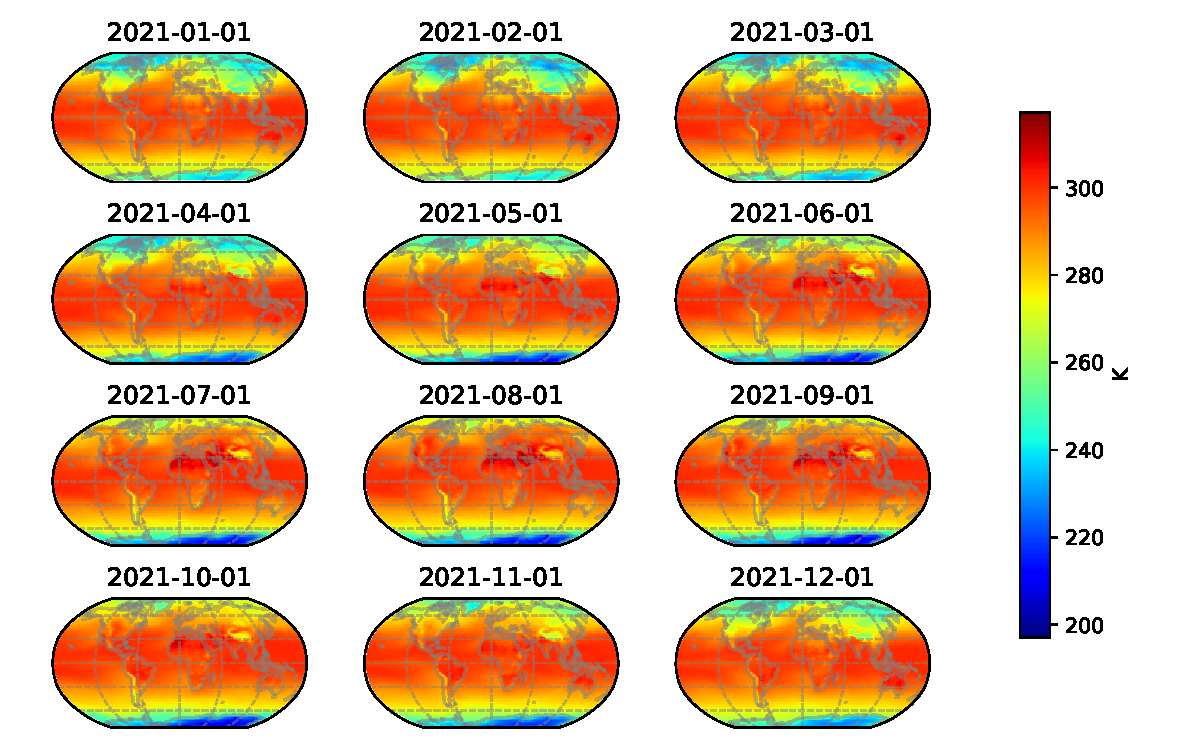
\includegraphics[width=1.0\textwidth]{cesm_temp_example}
	\caption[The average monthly temperature from the CESM-LE dataset.]{Monthly average temperature over the globe in Kelvin ($\si{\kelvin}$) from a single simulation from CESM-LE. The figure illustrates both the temporal and spatial dependency that is observed in temperature across the globe. The figure is projected to the Robinson projection for illustration purposes.}
	\label{fig:cesm_example}
\end{figure}

The CESM data is generated through simulations of a complex model of the Earth (see Section~\ref{sec:cesmle} for more detail).
However, EO data is also becoming more frequently generated through remote sensing.
Remote sensing is the monitoring of a physical characteristic of an area through measuring its reflected and emitted radiation at a distance. 
Space borne remote sensing, typically achieved through the use of satellite based sensors, is becoming more prominent as a source of EO data and in particular as a source of climatology data.
The three studies above, \citep{muro_short-term_2016, raspini_continuous_2018, khabbazan_crop_2019}, use space borne remote sensing to observe their process of interest. 
This is largely due to the increase in satellites launched which have been designed to capture various processes of the earth.
Figure~\ref{fig:sar_timeline} highlights the rise in availability of a single type of remote sensing satellite.
One particularly prominent remote sensing system is the European Space Agency's Sentinel Constellation, \cite{aschbacher_european_2012}.
The Sentinel constellation of satellites provides a wide range of remote sensing sensors which are easily accessible.
The constellation provides capabilities to capture various physical characteristics through the many forms of sensors equipped to its satellites.
These include  Synthetic Aperture Radar (SAR), optical and multispectral sensors.
For example, European Space Agency's Sentinel-4 from the Sentinel constellation, \cite{aschbacher_european_2012}, provides observation dedicated to air quality monitoring.
As such the Sentinel constellation has been widely used in EO studies; the three studies above, \citep{muro_short-term_2016, khabbazan_crop_2019, raspini_continuous_2018}  all utilise the Sentinel 1 SAR sensors for their observation source. 

\begin{figure}[htbp!] 
	\centering    
	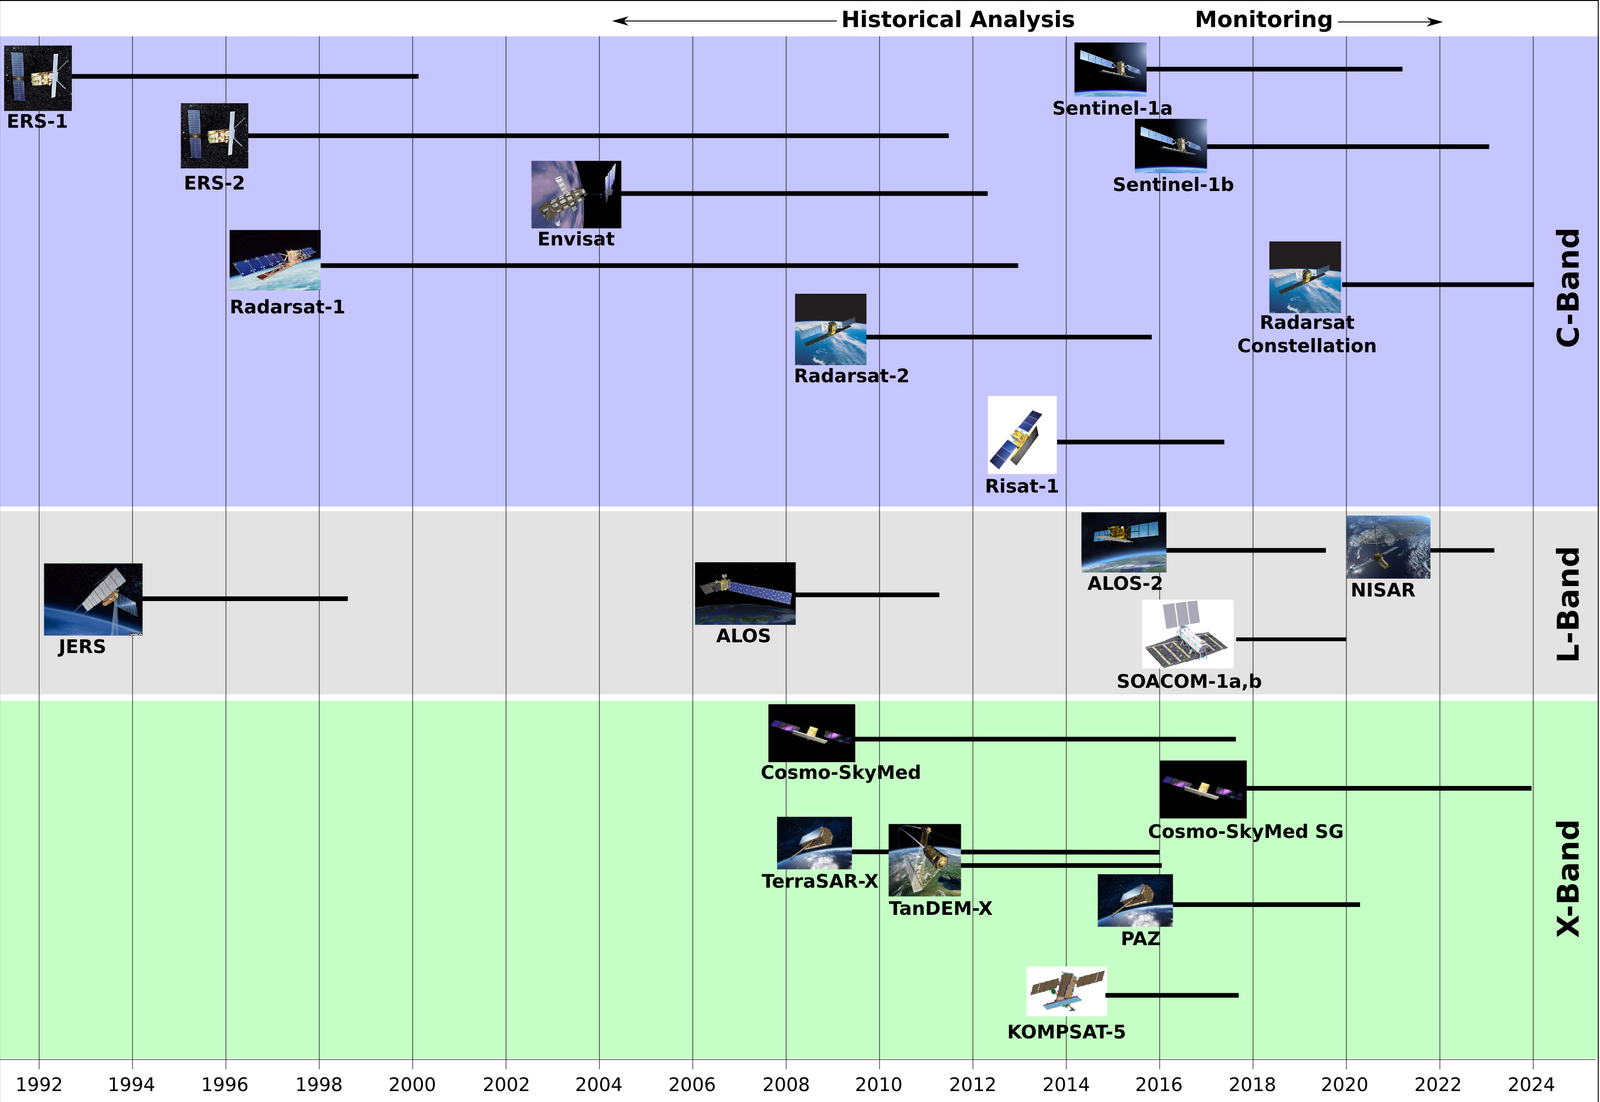
\includegraphics[width=1.0\textwidth]{Sensors}
	\caption[Timeline of the major EO satellite launches and operation time scales.]{A timeline of major satellite launches and operating periods for EO missions using SAR based sensors. This highlights the rapid rise in availability of such remote sensing capabilities, driven by the demand for observations to cover large spatial and temporal scales in areas such a climatology. The C, L, X band refers to the type of SAR sensor equipped to the satellite which are used in different applications. See \citep{oliver_understanding_2004} for details.}
	\label{fig:sar_timeline}
\end{figure}

A prominent focus of the Sentinel satellite constellation is to provide repeated observations at relatively high frequency, \cite{aschbacher_european_2012}.
This is in response to the rising demand for monitoring EO processes over time.
High frequency revisit times have been made possible by the development of remote sensing technologies.
For example, the Sentinel 1 satellite constellation can provide revisit times of approximately five days for areas of Europe.
Such short revisit times are advantageous as they give higher temporal resolution and thus studies can incorporate this additional information.
For example, \citeauthor{raspini_continuous_2018} utilise this in their study of land deformation change to identify anomalous regions, \citep{raspini_continuous_2018}.
The increasing availability of high temporal frequency EO data such as those provided by the CESM-LE dataset or the Sentinel satellite constellation thus drives a demand for statistical models which can handle both high resolution spatial and temporal dependency.  

Earth observation data, such as those provided by the CESM model or through remote sensing, have an inherent spatial and temporal dependency.
That is to say the underlying process driving both remotely sensed observations of the Earth and the CESM simulations will vary over the globe and also will be driven by the state of the system at prior time points.
That is not to say the process is the same for both but rather that there is a commonality in that they could both be considered spatio-temporal processes.
In addition there are more concrete similarities in the collection of such EO data.
Typically, EO data are described on a lattice of points over space which is usually regular.
This usually relates to the pixels of an image over the area of interest.
Such a lattice is represented through a geodetic coordinate system which grounds a datum to a real world location.
Finally, EO data typically have repeated observations through time over the same space.
This usually relates to the repeated imaging of the same area of interest at multiple points in time.

The description of such spatio-temporal processes is well studied in statistics and a large amount of effort has been used to develop various models to suit them.
A well known monograph which deals with such processes is that written by \citeauthor{cressie_statistics_2011}, \cite{cressie_statistics_2011}.
The monograph details various forms of spatio-temporal processes and typically focuses on the extension of spatial methods to incorporate the additional temporal dimension.
We discuss these methods in more detail in Section~\ref{sec:st_methods}.
Of particular importance in these methods is that temporal and spatial dimensions are treated distinctly as they are inherently different in the physical process.
For example, one could consider a spatial point influencing its neighbours in all directions however a temporal point reasonably shouldn't influence its past.
As such there is often a distinction in the method used to model the temporal and spatial aspects of the physical process.

An area of statistics which is often used to model data with temporal dependency is Functional Data Analysis (FDA).
FDA is typically applied to analyse data which vary over a continuum, \citep{ramsay_functional_2010}.
Time is one such continuum.
EO data with high frequency temporal observations are therefore suitable candidates for FDA models.
FDA is a relatively new branch of statistics and as such few studies have been presented which use FDA techniques on EO data.
\citeauthor{liu_functional_2012} consider FDA techniques on periodic EO data, \citep{liu_functional_2012}. 
Similarly \citeauthor{hooker_maximal_2015} consider FDA techniques to model the Harvard modified vegetation index sourced from EO data.
In both the above studies they consider EO data as a collection of functional observations indexed by space where each functional observation represents a trajectory over time.

The monograph of \citeauthor{ramsay_functional_2010} provides a comprehensive introduction to the themes of FDA, \citep{ramsay_functional_2010}.
FDA are often intuitive since viewing responses as being trajectories from an unknown smooth random function in some contexts closely matches the actual data generating process compared to a multivariate analysis.
The use of such techniques therefore could be helpful in modelling such high frequency EO data in conjunction with the multivariate methods discussed by \citeauthor{cressie_statistics_2011} in \citep{cressie_statistics_2011}.
However, focus in the FDA literature to date has primarily revolved around independently observed functional data.
This is typically not the case in our motivating case of EO data where there is often obvious spatial dependency.
Thus there is a need to describe functional data models which incorporate dependency among observations.
In this work we consider developing such models for dependent functional data with a focus on application to EO data.
We consider adapting well studied FDA methodologies and borrow techniques from spatio-temporal statistics to allow for spatially dependent observations.
In Section~\ref{sec:fr} we make concrete our definition of functional data. 

\section{Functional Representation \label{sec:fr}}
As mentioned in Section~\ref{sec:eo} EO data can be viewed as a collection of functional data.
However, there is a choice about how we interpret observations in this collection.
We may consider the data as a collection of functional observations with time being our functional dimension and space our collection dimension.
For example, we may consider each spatial location from Figure~\ref{fig:cesm_example} giving rise to a trajectory over time of which we have only observed 12 time points.
Or we may consider the functional observations having a spatial domain and the collection dimension being time.
That is we may consider each image in Figure~\ref{fig:cesm_example} being a surface with observations only at pixel locations and the collection consists of a time series of such surfaces. 
The canonical presentation of functional data in FDA is to use time as the functional dimension, \citep{ramsay_functional_2010}, and thus we use the below definition of functional data from this point of view. 

\subsection{Functional data \label{ssec:fd}}
Multivariate data analysis usually revolves around the study of observations which are finite dimensional and is well studied.
Modern data collection techniques can now create data which are extremely numerous and thus can often be viewed as functions.

For example, \citeauthor{ferraty_nonparametric_2006} consider the case where we can observe a random variable at several times between some minimum and maximum time, $\left( t_{\text{min}}, t_{\text{max}} \right)$, \citep{ferraty_nonparametric_2006}.
A single observation can then be considered as the collection $ \{ X(t_j) ; j=1,2,\dots, J\}$ where $J$ is the total number of temporal sample points and $X(t)$ is the response variable at time $t$.
Unlike multivariate data we consider the case that the separation between observations becomes minimal.
That is we consider the data as an observation from the continuous random process $\mathcal{X} = \{X(t); t \in \left( t_\text{min}, t_\text{max} \right)\}$.
We therefore propose as in \citep{ferraty_nonparametric_2006} and \citep{shi_gaussian_2011} the following definition of a \textit{functional variable}.

 \begin{definition}[Functional Variable]
	A random variable $\mathcal{X}$ is called a functional variable if it takes values in an infinite dimensional space (or functional space). Observations $\chi$ of $\mathcal{X}$ are called a functional data.
	\label{def:functional_variable}
\end{definition}

Further to this, suppose we observe a collection of functional data (realisations of $\mathcal{X}$).
Then we will denote this collection by the term \textit{functional dataset}.

\begin{definition}[Functional Dataset]
	A functional dataset, $\chi_1, \chi_2, \cdots, \chi_N$ is the collection of $N$ realisations of functional variables $\mathcal{X}_1, \cdots, \mathcal{X}_N$ identically distributed to $\mathcal{X}$.
	\label{def:functional_dataset}
\end{definition}

The canonical way to present functional data and the subsequent methods is to use time as the continuous variable, \cite{ramsay_functional_2010, ferraty_nonparametric_2006, shi_gaussian_2011}, as described above.
However, there is no such restrictions in either Definition~\ref{def:functional_variable} or Definition~\ref{def:functional_dataset}. 
In fact, another case is to consider the functional domain of the variables to be space.
In our proposed methodologies we present when possible with respect to time due to the simplification it brings in notation.
We will make explicit reference when we change the domain of our functional data, for example if we consider space as our continuous domain. 

We introduce the following notation for use in the remainder of this work.
We consider our EO dataset to be observed in some spatial domain with dimension $p$, which we denote by $\mathcal{S} \subset \mathbb{R}^p$, and temporal domain donated by $\mathcal{T} \subset \mathbb{R}$.
Typically $p$ will be two or three since these represent the space of common spatial domains in EO data.
Any observed dataset we can enumerate with one index over the spatial location and the other indexing the temporal locations.

We assume our dataset is comprised of $N$ spatial locations and let $\ve{s}_i \in \mathcal{S}$ be the spatial location of the $i^\text{th}$ observed functional variable.
At each spatial location we suppose we observe $J_i$ temporal observations and denote by $t_{ij} \in \mathcal{T}$ the $j^\text{th}$ temporal observation of the $i^\text{th}$ functional variable.
Then our dataset can be summarised by $Y$ where:
\begin{equation}
	Y = \{ y_{ij}; i=1,2,\cdots,N, j=1,2, \cdots, J_i \}
	\label{eqn:observed_data}
\end{equation}
where $y_{ij}$ is the response value of the $i^\text{th}$ functional variable at time $t_{ij}$ observed with error.
That is we consider for each spatial location the discrete temporal observations being a sample from a realisation of a functional variable observed with error.
That is:
\begin{equation}
	y_{ij} = \chi_{i}\left( t_{ij} \right) + \varepsilon_{ij}
	\label{eqn:fd_temporal}
\end{equation}
where, as in Definition~\ref{def:functional_dataset}, $\chi_i$ is a realisation of functional variable $\mathcal{X}_i$ for $i=1,2,\cdots,N$.
We consider each functional variable as being identically distributed as $\mathcal{X}$.
As is common in most observation models, we assume that we observe data with error.
Typically one assumes that the error process $\{\varepsilon_{ij}; i=1,2,\cdots,N, j=1,2,\cdots,J_i\}$ is a white noise process with variance $\sigma_\varepsilon^2$. 

In this case one considers the modelling of the EO dataset by ensuring smoothness of some kind over the temporal domain via its functional data representation.
We can then consider building in spatial dependency by assuming a sampling correlation in our $N$ functional data.
An area where such spatial dependency has been long studied is multivariate spatio-temporal methods.

\section{Spatio-Temporal Methods \label{sec:st_methods}}
In the statistical literature spatial and spatio-temporal models have been extremely well studied, especially due to the prevalence of geo-statistical applications.
In the following we briefly review some of the most commonly observed spatial and spatio-temporal statistical models in the multivariate analysis literature. 

The monograph of \cite{cressie_statistics_2015} and references within provide a succinct summary of traditional methodologies in spatial statistics; many of which are applicable to EO data.
Generally speaking, spatial data can be split into one of three categories; geo-statistical, area, and point process data, \citep{cressie_statistics_2015}.
In this work the EO data described in Section~\ref{sec:eo}  are most suitably modelled using geo-statistical models.
The canonical model used in geo-statistical settings is the Kriging model.
The Kriging model is well described in \cite{stein_interpolation_1999}.
Such models treat spatial data as samples from a random spatial process and predictions for unknown values can be calculated from a weighted combination of known values in a neighbourhood of our unknown location utilising the correlation among neighbouring points.
A prime example of the spatial Kriging model in use for EO data is given in \cite{rossi_kriging_1994}.
Extensions to the basic Kriging technique have also been employed across a number of geo-statistical settings, including Co-Kriging involving extra covariate information for reconstruction, \cite{zhang_restoration_2009}.
Kriging is well known in many fields through various names, in the FDA literature it is most often referred to as Gaussian processes regression.
\citeauthor{shi_gaussian_2011} describe in detail the concept of Gaussian processes in the context of functional regression, \citep{shi_gaussian_2011}, and we discuss them more in Section~\ref{sec:gp}. 

As is detailed in \cite{cressie_statistics_2015} a key aspect to geo-statistical modelling is the specification of spatial dependency in the observed data.
A common way for such specification is through parametric covariance or kernel functions.
Traditional stationary parametric functions such as the Mat\`{e}rn covariance are discussed in detail in \cite{cressie_statistics_2015}.
These commonly rely on the assumption of isotropy and stationarity in modelling which rarely holds in practice.
Further literature has considered extensions of these and is in fact an active area of research.
\citeauthor{schmidt_flexible_2020} compare a variety of methods for producing non stationary and heterogeneous covariance structures for the goal of spatial interpolation, \citep{schmidt_flexible_2020}.
They group the various methods of creating such structures into four categories; deformation, convolution, covariate, and stochastic partial differential equations.
The deformation approach proposed by \citeauthor{sampson_nonparametric_1992} extends the anisotropic stationary covariances, such as those described in \cite{cressie_statistics_2015}, by allowing for a non linear transformation to the space which creates a latent space where isotropy holds, \cite{sampson_nonparametric_1992}.
The convolution approach proposed by \citeauthor{higdon_space_2002} uses a specific form of the covariance kernel which can be represented as a convolution between a convolution kernel and a white noise process.
We discuss such an approach more in Chapter~\ref{cha:cpace}.
The covariate based approach to constructing non stationary kernels tends to use an adaption to the convolution or deformation approaches with specific covariates, \citep{schmidt_flexible_2020}.
Finally the stochastic partial differential equation method proposed by \citeauthor{lindgren_explicit_2011} construct non stationary covariances through formulating the resulting Gaussian process as the solution of a stochastic partial differential equation which guarantees the construction of a well defined covariance function, \citep{lindgren_explicit_2011}. 

A natural extension to purely spatial modelling of spatio-temporal data is to include the temporal domain.
Such models are known as spatio-temporal models.
Spatio-temporal models are well discussed in the monograph \cite{cressie_statistics_2011} by \citeauthor{cressie_statistics_2011}.
Spatio-temporal Kriging models are well suited to EO data; however these models are relatively scarce in the literature.
\citeauthor{militino_introduction_2018} considers the application of such modelling in the satellite remote sensing literature and reasons the lack of them is primarily due to the added complexity these models produce in specifying valid space-time covariance functions, \cite{militino_introduction_2018}.
As such, one particular direction spatio-temporal modelling has considered is the creation of spatio-temporal covariance functions.
Spatio-temporal covariance functions are discussed in \citep{cressie_statistics_2011}.
Separability between spatial and temporal correlations is often a key assumption in some methods due to the reduction in computational complexity they provide.
The separability assumption proposes that a space-time covariance function $k(\ve{s}, t, \ve{s}^\prime, t^\prime)$ can be factored into two separate covariance functions $k_{s}(\ve{s}, \ve{s}^\prime)$ and $k_t(t, t^\prime)$, one for each of the spatial and temporal dimensions. 
In particular for EO data, \cite{george_selecting_2015} consider the selection of separable covariances and \cite{deb_spatio-temporal_2019} consider such models for air pollution data. 
However, the separability assumption may be too restrictive for capturing complex spatio-temporal processes, \citep{cressie_statistics_2011}. 
As such \citep{mitchell_likelihood_2006, fuentes_testing_2006, aston_tests_2017} considers tests for when the separability assumptions hold.
The work in \citep{cressie_classes_1999, gneiting_nonseparable_2002, iaco_nonseparable_2002} consider the construction of non separable covariance functions for when separability doesn't hold for use in spatio-temporal models.

\section{\label{sec:summary_research}Summary of Research}
The motivation of this work is to provide a model designed for EO data which provides an explanation of both the spatial and temporal process in a parsimonious way.
We present a novel method named Correlated Principal Analysis through Conditional Expectation (CPACE), that is designed for modelling EO data.
The model builds upon existing FDA techniques to extend modelling from independently observed functional data to functional data which exhibits spatial correlation.
The emphasis in this work is to utilise the FDA paradigm over the temporal domain to aid in the decomposition of the data; with the understanding that our data generating process is smooth across the temporal domain.
Such a decomposition gives a parsimonious description of the data with respect to its temporal domain by describing its principal modes of variation.
We then estimate a spatial correlation structure for each component using well known spatial statistical methods.
The combination of the resulting estimated spatial covariance structures with the principal directions aims to capture the majority of temporal and spatial dependency observed in the data.
We can then utilise the CPACE model to help predict responses at unseen spatial and temporal locations, which is an area of keen interest in EO studies.
We assess our model using various simulated data both with known correct data generating distribution and to simulations drawn from an incorrect data generating procedure.
We apply our CPACE model to selected atmospheric variables from the CESM dataset as an example application of the model to EO data.

The work is structured as follows.
In Chapter~\ref{cha:data} we describe our example datasets which we use to illustrate the performance of the model.
In Chapter~\ref{cha:background} we present the methodologies underpinning the CPACE models, these are typically well known FDA and spatio-temporal statistical methods.
We also present the smoothing methodologies used to estimate the mean and covariance surfaces of our random functional variables.
In Chapter~\ref{cha:ftsm} we present an interim model built on the combination of two well known existing methodologies in the FDA literature with a focus on application to an EO dataset.
Such a model proposes a novel approach to modelling EO data and helps to highlight the need to include both spatial and temporal effects in modelling such data.
In addition, the proposed model in Chapter~\ref{cha:ftsm} gives an opportunity to explore EO data where the functional domain is space rather than time.
We present the benefits and limitations of such an approach in practice in this chapter.
In Chapter~\ref{cha:cpace}, we introduce the main contribution of this work; which is the CPACE model for correlated functional data.
We describe the model in detail as well as providing asymptotic results.
In Chapter~\ref{cha:application}, we apply the CPACE model to simulated data and in Chapter~\ref{cha:real_application} to real world datasets.
Simulation results are presented with comparisons to various existing models with a focus on comparative ability to recover known data generating parameters.
Applied results to real world datasets are included with comparisons to existing techniques; with a focus on interpolation and forecasting abilities of the model.
In Chapter~\ref{cha:implementation}, we highlight the practical difficulties in implementing the model, with discussion on various techniques which are used to overcome the high dimensionality which is typical in the EO data.
Finally, in Chapter~\ref{cha:conclusions} we draw the conclusions of the work and present areas of possible further work.
%!TEX root = ../thesis.tex
%*******************************************************************************
%*********************************** Second Chapter *****************************
%*******************************************************************************

\nomenclature[z-TMQ]{TMQ}{Total vertically integrated precipitation from CESM-LE.}
\nomenclature[z-PS]{PS}{Pressure at reference height of $2\si{\meter}$ from CESM-LE.}
\nomenclature[z-TREFHT]{TREFHT}{Temperature at reference hieght of $2\si{\meter}$ from CESM-LE.}
\nomenclature[z-U10]{U10}{Wind speed at height of $10\si{\meter}$ from CESM-LE.}
\nomenclature[z-CESM-LE]{CESM-LE}{Community Earth System Model - Large Ensemble.}

\chapter{Data Sets\label{cha:data}}  %Title of the Second Chapter

\ifpdf
    \graphicspath{{Chapter2/Figs/Raster/}{Chapter2/Figs/PDF/}{Chapter2/Figs/}}
\else
    \graphicspath{{Chapter2/Figs/Vector/}{Chapter2/Figs/}}
\fi

In the following chapter we describe in detail our data which we will use as a source for assessing the performance of the models described within.
We use a publicly available set of climate model simulations known as the CESM Large Ensemble (CESM-LE) data set, \citep{kay_community_2015}.
The CESM-LE data set provides a good example of EO data that is discussed in Section~\ref{sec:eo}. The data set is publicly available from \url{https://www.cesm.ucar.edu/projects/community-projects/LENS/data-sets.html}.

 \section[CESM-LE]{\label{sec:cesmle}Community Earth System Model - Large Ensemble}
 The CESM-LE data set is an extremely popular and significant data set in the climate research community.
 It was developed to enable the assessment of recent past and near future climate change in the presence of internal climate variability, \citep{kay_community_2015}.
 It does so by providing $40$ simulations of a complex climate model where each simulation is subject to the same radiative forcing scenario but initialised from a slightly perturbed atmospheric state.
 As such the forty resultant simulations present the various trajectories the model might take due to internal climate variability of the model. 
 
 The model used to run the forty member ensemble is the Community Earth System Model version 1, \citep{hurrell_community_2013}, with the Community Atmosphere model version 5, \citep{hurrell_community_2013}, as the atmospheric component.
 The model is a fully coupled climate model which consists of a model for each of land, ocean, atmosphere and sea ice components of the climate.
 These are brought together with a coupler model.
 Figure~\ref{fig:cesm} provides a simple overview as to how CESM model couples the various components.
 Such a model is capable of simulating various Land, Ocean, Atmosphere and Sea Ice variables of the climate, such as the wind speed, temperature or pressure.
 The CESM-LE produces simulations of such variables on the nominal $1\deg$ horizontal separation across the globe which induces our spatial resolution of the data.
 The ensemble produces variables at three different levels of temporal resolution between the years 1920 and 2100 for non-control simulations. The ensemble is able to produce variables at 6-hourly, daily, and monthly intervals. 
 
 \begin{figure}[htbp!] 
 	\centering    
 	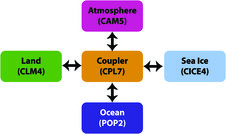
\includegraphics[width=1.0\textwidth]{cesm_components}
 	\caption[CESM component models]{The component models for the full CESM model, Figure from \citep{kay_community_2015}. The individual component models are atmospheric (CAM5), ocean (POP2), land (CLM4), Sea Ice (CICE4), and coupler (CPL7). Details of which can be found in \citep{kay_community_2015} and \citep{hurrell_community_2013}.}
 	\label{fig:cesm}
 \end{figure}

 For this body of work we use the CESM-LE data by considering the forty members as separate simulations.
 Each simulation represents a single realisation of the various climate variables generated by the model described in \citep{kay_community_2015} where the variation between realisations is coming from the internal climate variability. 
 We apply a set of preprocessing to the raw data provided by the CESM-LE model as described below. 
 
 \subsection{Preprocessing \label{sec:preprocessing}}
 The full CESM-LE data consists of a large number of climate variables on a relatively large spatial grid consisting of $192 \times 276$ locations and as such is a rather large data set. 
 The main goal in our preprocessing is to reduce the size of the data through a series of variable selection, spatial resampling, and temporal sectioning.
 We reduce the data size by considering only a subset of the full data set by selecting four variables to study from the full model which are; temperature, pressure, wind speed, and precipitation. 
 The next preprocessing step we use is a temporal cut.
 We consider only the output of the CESM-LE which occurs between December 2020 and January 2026. 
 These time points were chosen such that the length of time gave reasonable ability to capture periodic elements but that the size of the data did not become too large.
 By using monthly frequency observations and this five year time horizon we have a sixty temporal observations for each spatial grid point and for each of our four variables considered. 
 
 The final step in our preprocessing pipeline is to reduce the spatial dimension.
 To do this we resample the model simulations to a smaller spatial grid for each variable of interest.
 Resampling is achieved by averaging values of neighbouring locations until our desired resolution is achieved.
 In this case we resample until the spatial size of the data set is $64 \times 96$ which corresponds to a reduction factor of $3$ from the original CESM-LE data.
 Figure~\ref{fig:cesm_grid} shows the comparison between the full and resampled spatial observation grid over the globe due to our preprocessing step
 The figure uses the temperature variable as at January 2021 as an illustrative example. 
 Obviously using such an approach reduces the spatial resolution and thus our ability to see small scale spatial patterns.
 However, this is traded off against agility in terms of modelling due to the reduced data size.
 The reduction factor of $3$ was chosen based on this trade off.
 
 \begin{figure}[htbp!] 
 	\centering    
	\begin{subfigure}[b]{0.45\textwidth}
		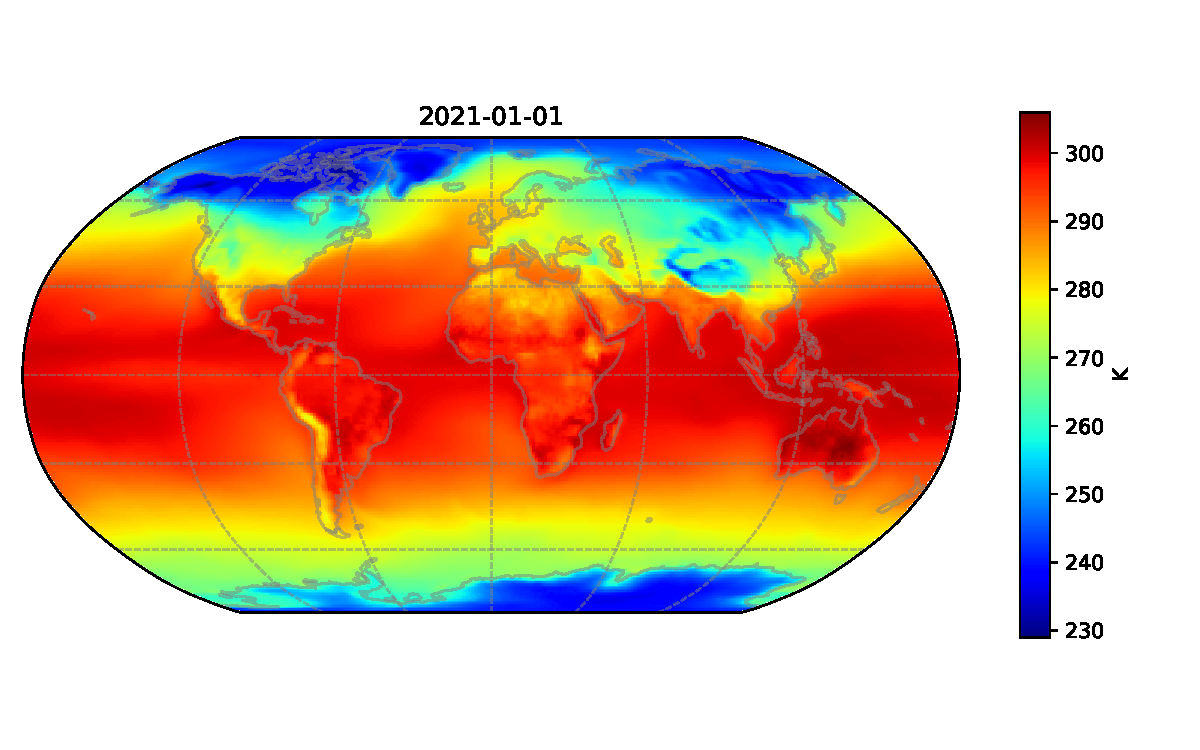
\includegraphics[width=\textwidth]{full_grid}
		\caption{Full resolution.}
		\label{fig:full_res}   
	\end{subfigure}             
	\begin{subfigure}[b]{0.45\textwidth}
		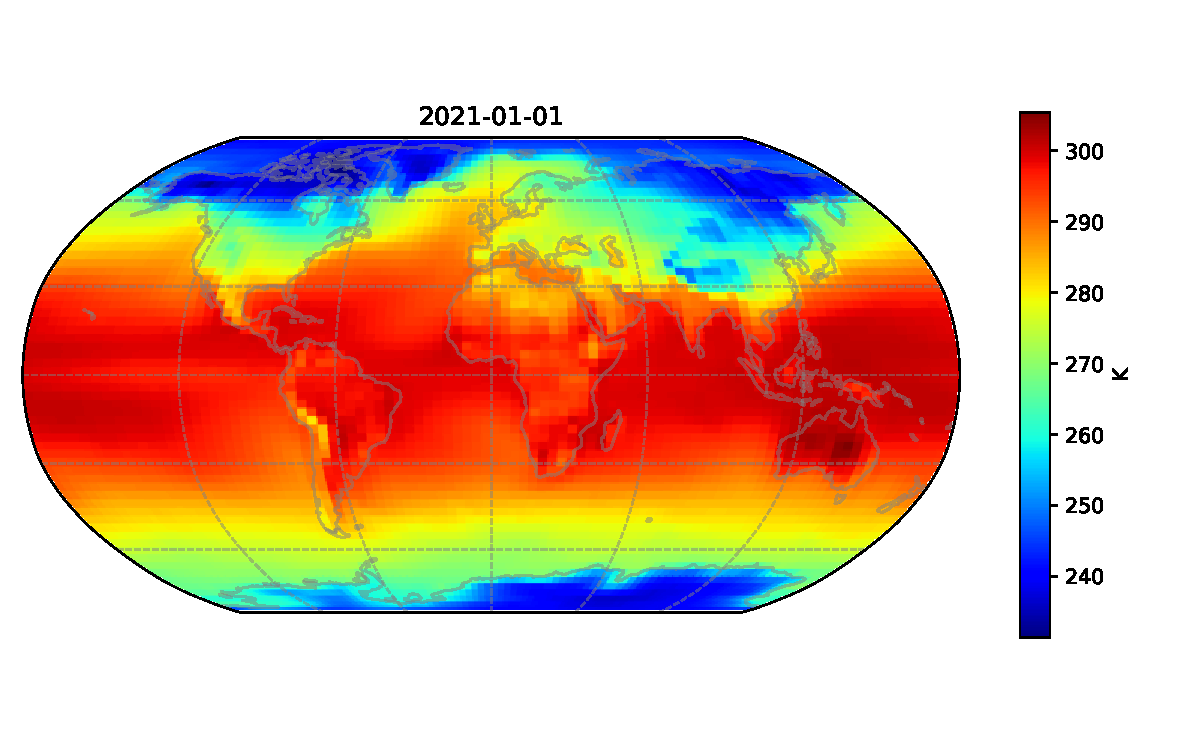
\includegraphics[width=\textwidth]{coarse_grid}
		\caption{Reduced resolution.}
		\label{fig:coarse_res}
	\end{subfigure}             
 	\caption[CESM-LE resampled spatial grid after preprocessing]{The resampled spatial grid of observation measurements across the globe. Notice the reduced spatial resolution in Figure~\ref{fig:coarse_res} compared to that in Figure~\ref{fig:full_res} due to the resampling causing some loss of fine spatial detail. Example used is the average monthly temperature in Kelvin ($\si{\kelvin}$) on January 2021.}
 	\label{fig:cesm_grid}
 \end{figure}

 \subsection{Variables \label{ssec:variables}}
 In the following section we focus our description to the four atmospheric model variables from the  CESM-LE simulations that we will use in this body of work.
 These are; pressure, temperature, precipitation, and wind speed.
 We describe each variable in detail in their respective section and throughout this work we consider each as a separate EO data set.
 We aim to show, through the use of an example time point and spatial locations, the various spatial and temporal processes that exist in each of these variables.
 These make such a data set a credible EO data set to test our proposed CPACE model on. 

\subsubsection{Precipitation \label{sssec:precip}}
The total (vertically integrated) precipitable water component abbreviated as TMQ is an atmospheric component output of the CESM-LE, \citep{kay_community_2015}.
The variable is given units of $\si{\kilogram\per\metre\squared} $ and is available monthly on the full spatial grid.
The monthly precipitation is calculated as the average over time from the  CESM-LE model six hourly output. 

We can see clearly the spatial variability of the precipitation over the globe by considering the heat map of June 2021 monthly precipitation for a single simulation; which is shown in Figure~\ref{fig:precip_june}. 
As one would expect there is clear spatial correlation.
For example, the tropics observe large amounts of precipitation whereas desert regions observe little. 
We can also see some subtler differences in the spatial correlation structure. 
Figure~\ref{fig:precip_june} shows that bands of precipitation are evident over the globe.
This indicates that precipitation is much more correlated over lines of latitude than lines of longitude. 
This may be an indicator of spatial anisotropy in the generating process.
There is also a case of observing more complex, possibly non stationary, spatial processes as the correlation structure seems different between say North America and Indonesia. 
We can similarly observe clear temporal correlations in the precipitation variable of the CESM model.
In particular, Figure~\ref{fig:precip_temp} shows the time series of two locations; the United Kingdom (UK) and Colombia.
Each exhibit clear periodic signals as wet seasons and dry seasons repeat each year.
However, we can see a clear level difference between the UK and Colombia precipitation as well as differences in the range of precipitation.
This highlights the fact that not only do we have temporal correlation but this correlation is dependent on location. 

\begin{figure}[htbp!] 
	\centering
	\begin{subfigure}[b]{0.45\textwidth}
		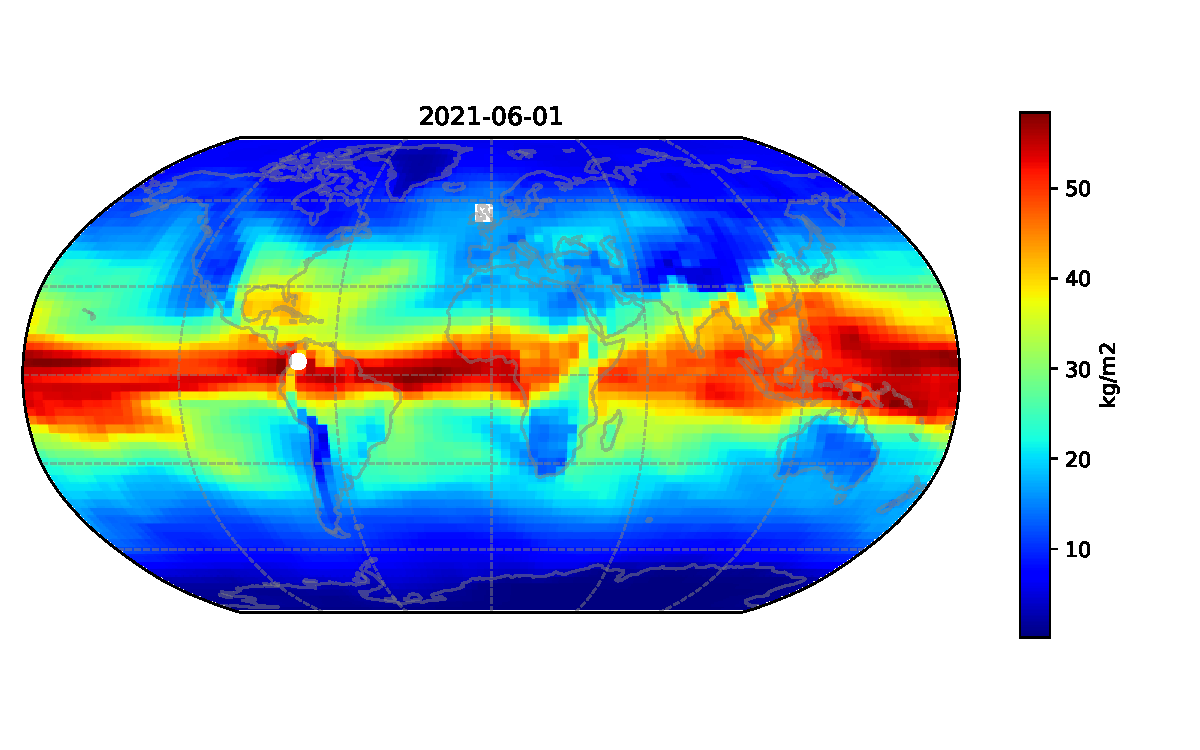
\includegraphics[width=\textwidth]{TMQ_example}
		\caption{TMQ as at June 2021.}
		\label{fig:precip_june}   
	\end{subfigure}             
	\begin{subfigure}[b]{0.45\textwidth}
		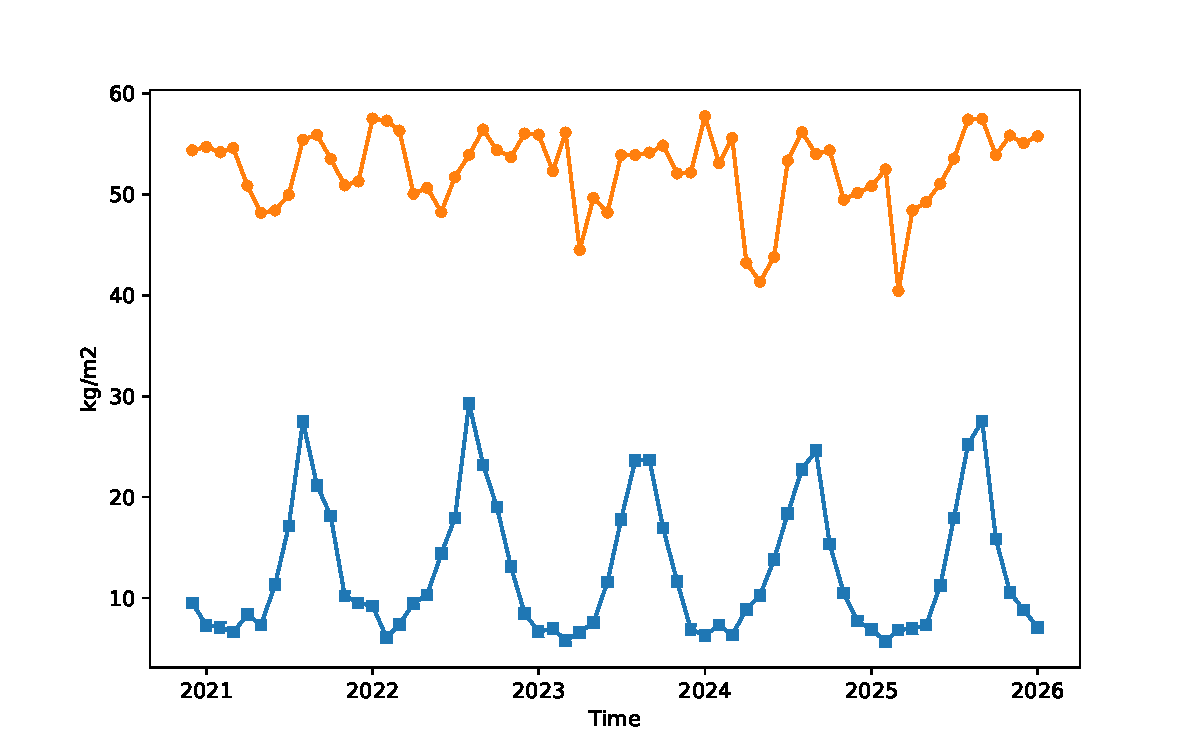
\includegraphics[width=\textwidth]{TMQ_example_temp}
		\caption{TMQ over time.}
		\label{fig:precip_temp}
	\end{subfigure}             
	\caption[Overview of Precipitation variable]{Overview of the monthly average precipitation variable (TMQ) from CESM-LE ensemble member 1. Figure~\ref{fig:precip_june} highlights the spatial correlation present while Figure~\ref{fig:precip_temp} highlights the temporal correlation at two distinct locations; namely Colombia and the United Kingdom. The orange circle and blue square markers mark these respectively on Figure~\ref{fig:precip_temp} with the white markers highlighting their locations in Figure~\ref{fig:precip_june}. Note the level difference in temporal correlation structure between the two locations, indicative of a spatio-temporal correlation process occurring.}
	\label{fig:precip_overview}
\end{figure}

\subsubsection{Pressure \label{sssec:pressure}}
The surface pressure variable abbreviated as PS is another atmospheric component output of the CESM-LE, \citep{kay_community_2015}.
The component is given in Pascals ($\si{\pascal}$) and represents the surface pressure at a height of $2\si{\meter}$. It is available monthly on the full spatial grid and the monthly average is calculated as the average over time from the CESM-LE model six hourly output.

Figure~\ref{fig:pressure_overview} gives a brief insight to this variable. 
We can see the spatial correlation structure of pressure over the globe in Figure~\ref{fig:pressure_june}.
One can clearly see areas of high and low pressure.
For example, there is a significant difference between the low pressure zone over Antarctica and high pressure zone over Australia. 
It is interesting to note that we see a clear difference in the smooth structure over sea and a rougher structure over land variables. 
This again might motivate that a non stationary spatial process is driving such a variable.
Considering the temporal variation displayed for Colombia and the UK in Figure~\ref{fig:pressure_temp}; we can see definite structure over time, albeit different for each location.
The UK exhibits much more variation in pressure than Colombia, however both do exhibit temporal correlation. 
Again, similar to the precipitation variable discussed in Section~\ref{sssec:precip}, this might suggest that modelling such a variable will need to consider both spatial and temporal correlations in conjunction with each other.

\begin{figure}[htbp!] 
	\centering
	\begin{subfigure}[b]{0.45\textwidth}
		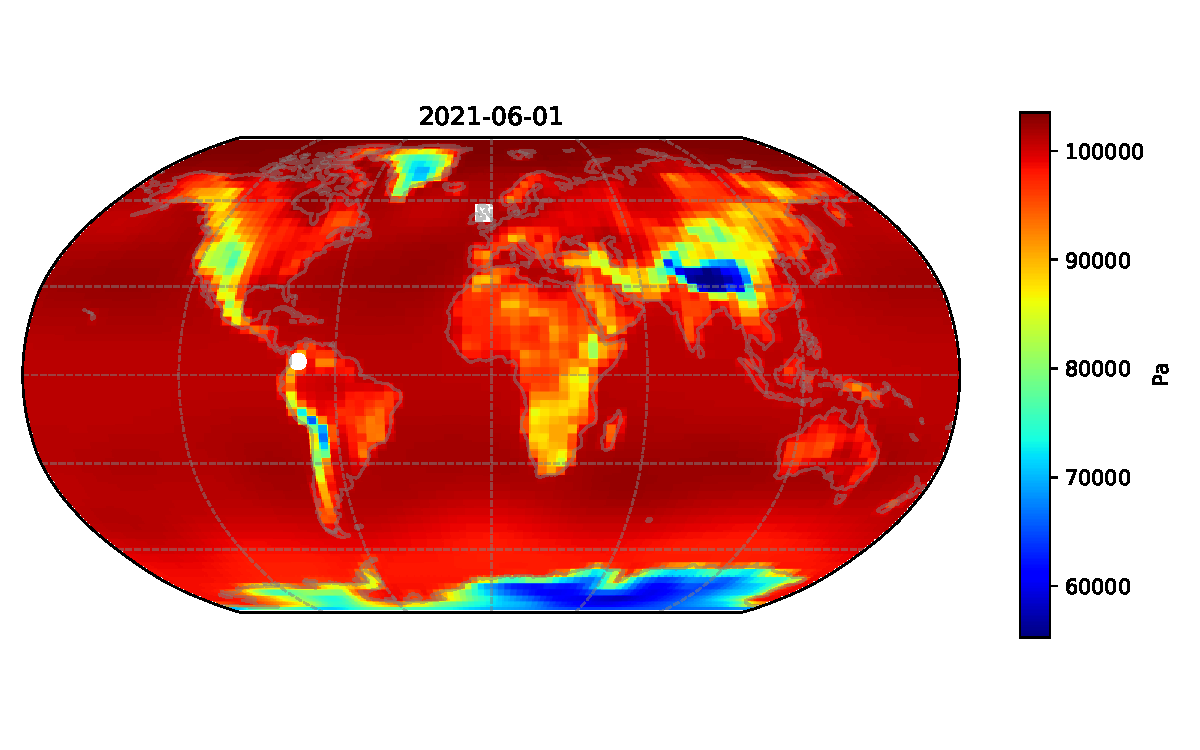
\includegraphics[width=\textwidth]{PS_example}
		\caption{PS as at June 2021.}
		\label{fig:pressure_june}   
	\end{subfigure}             
	\begin{subfigure}[b]{0.45\textwidth}
		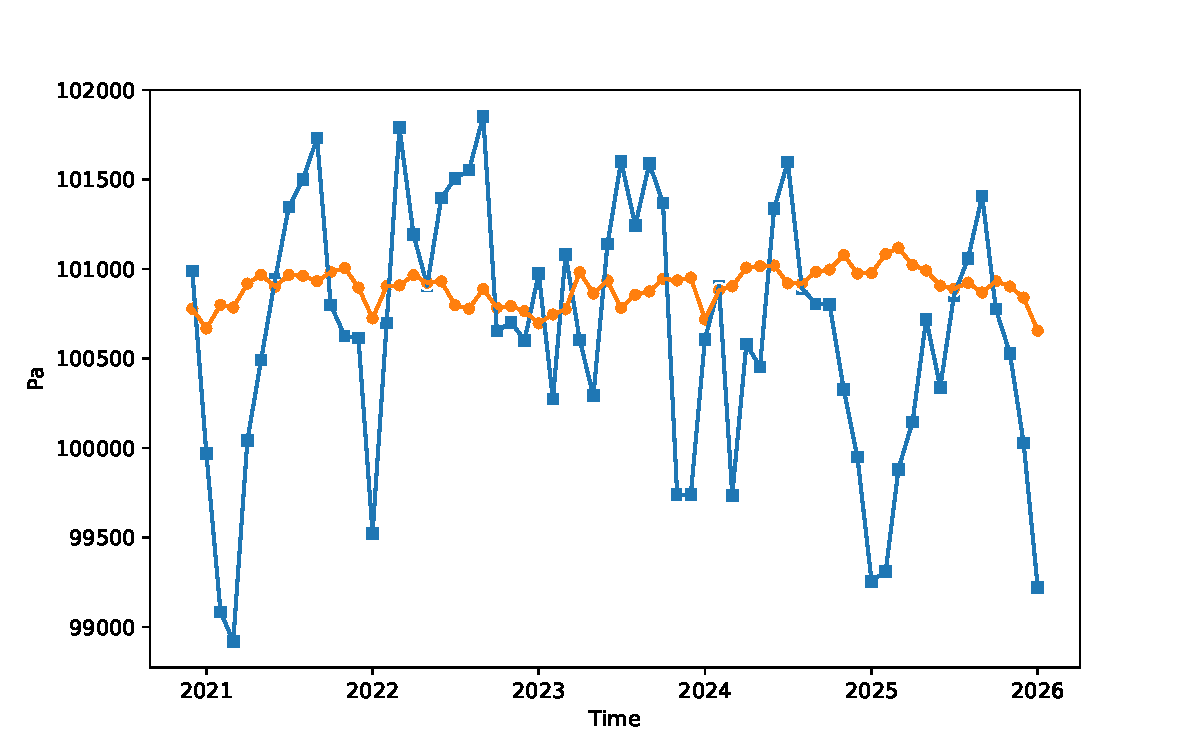
\includegraphics[width=\textwidth]{PS_example_temp}
		\caption{PS  over time.}
		\label{fig:pressure_temp}
	\end{subfigure}             
	\caption[Overview of Pressure variable]{Overview of the monthly average pressure variable from CESM-LE ensemble member 1. Figure~\ref{fig:pressure_june} highlights the spatial correlation present while Figure~\ref{fig:pressure_temp} highlights the temporal correlation at two distinct locations; namely Colombia and the United Kingdom. The orange circle and blue square markers mark these respectively on Figure~\ref{fig:pressure_temp} with the white markers highlighting their locations in Figure~\ref{fig:pressure_june}. Notice the stark difference between the time series variance in the UK and Colombia.}
	\label{fig:pressure_overview}
\end{figure}

\subsubsection{Temperature \label{sssec:temp}}
The temperature variable abbreviated to TREFHT is an atmospheric component output of the CESM-LE, \citep{kay_community_2015}.
The variable refers to the average temperature in Kelvin ($\si{\kelvin}$) at the model reference height which is $2\si{\meter}$ above sea level.
The average is available monthly with said average being calculated from the model six hourly output over the month.

Quite clearly the temperature exhibits spatial correlation across the globe and periodic signals through time the seasons unfold.
Figures~\ref{fig:temp_june},~\ref{fig:temp_temp} highlight this for the spatial and temporal correlation respectively.
Clearly the temperature at June increases as we move closer to the equator and decreases at the poles. 
Similarly to the precipitation, we observe that the spatial correlation structure is clearly anisotropic. 
Correlation is much more pronounced over longitude than latitude. 
Looking more deeply at Figure~\ref{fig:temp_overview} we can observe more complex correlation structures, as mentioned in Section~\ref{sec:eo}. 
For example, Asia exhibits a localised area of low temperature right next to an area of relatively high temperature. 
This is very different to the extremely smooth variation that we see over the larger oceans such as the Atlantic. 
Again similar to the previous variables, this is an indication that there may be a non-stationary spatial process helping to drive this variable.

Figure~\ref{fig:temp_temp} gives an insight into the temporal correlation structure in the variable for two locations; namely Colombia and the UK. 
There is strong evidence of a periodic signal driving both but clearly there is a level shift and change in amplitude for the two locations. 
This is again similar to the precipitation variable discussed in Section~\ref{sssec:precip} and motivates the idea that there is a clear spatio-temporal process driving the variable rather than just either temporal or spatial process.

\begin{figure}[htbp!] 
	\centering
	\begin{subfigure}[b]{0.45\textwidth}
		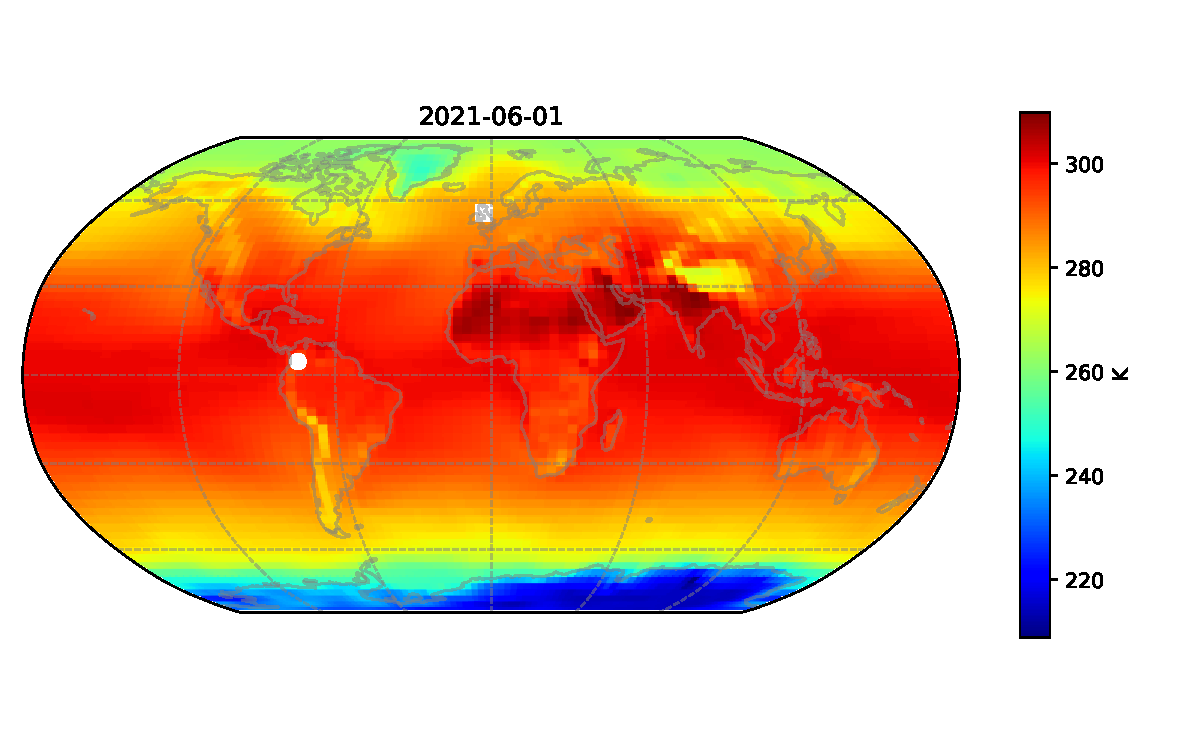
\includegraphics[width=\textwidth]{TREFHT_example}
		\caption{TREFHT as at June 2021.}
		\label{fig:temp_june}   
	\end{subfigure}             
	\begin{subfigure}[b]{0.45\textwidth}
		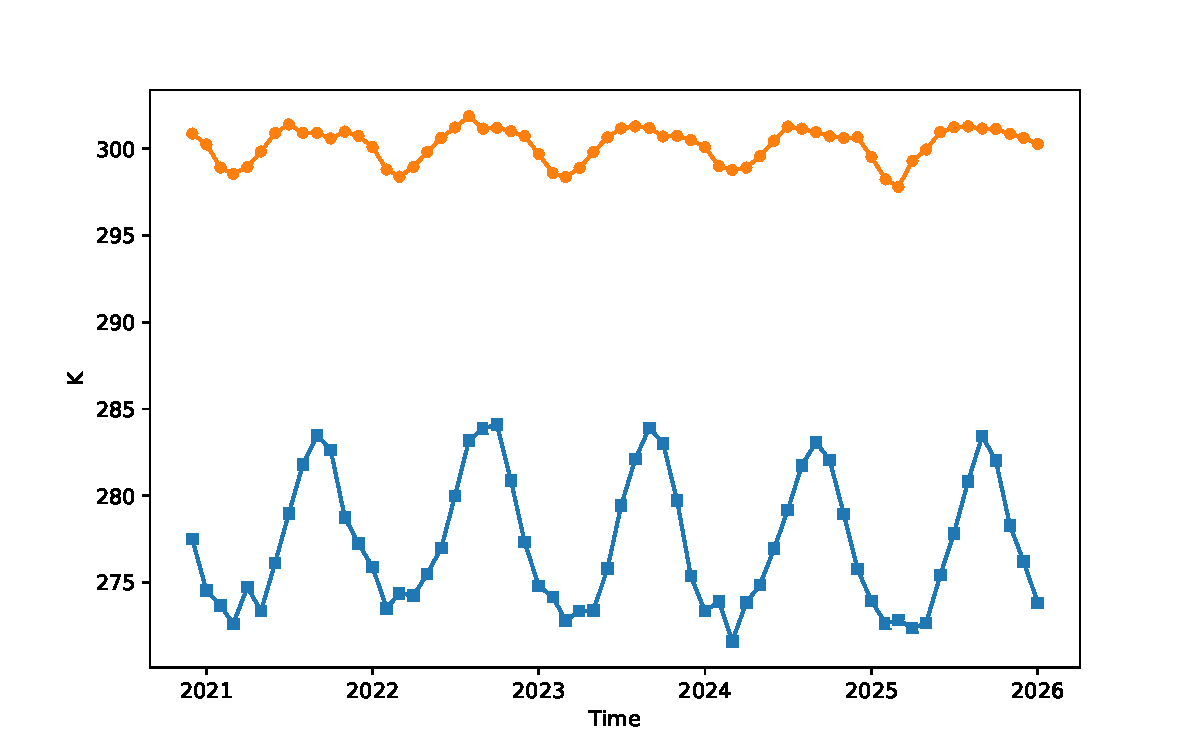
\includegraphics[width=\textwidth]{TREFHT_example_temp}
		\caption{TREFHT  over time.}
		\label{fig:temp_temp}
	\end{subfigure}             
	\caption[Overview of Temperature variable]{Overview of the monthly average temperature variable from CESM-LE ensemble member 1. Figure~\ref{fig:temp_june} highlights the spatial correlation present while Figure~\ref{fig:temp_temp} highlights the temporal correlation at two distinct locations; namely Colombia and the UK. The orange circle and blue square markers mark these respectively on Figure~\ref{fig:temp_temp} with the white markers highlighting their locations in Figure~\ref{fig:temp_june}.}
	\label{fig:temp_overview}
\end{figure}

\subsubsection{Wind speed \label{sssec:wind}}
The wind speed variable  abbreviated to U10 is another atmospheric component output of the CESM-LE model.
The variable refers to the average wind speed in $\si{\meter\per\second}$ at a height of $10\si{\meter}$ above sea level.
Again the variable is available on the full spatial grid and is available as a monthly average over time.

We visualise the spatial correlation of the variable in Figure~\ref{fig:wind_june} by considering a snap shot of the monthly average wind speed in June 2021.
We can see, in contrast to the previous three variables, that this has a much rougher spatial correlation structure over the sea. 
In fact it is interesting to observe the distinct difference in variability over the sea compared to that over the land. 
This may suggest that we have two types of correlation structure existing for this variable, one for the land and one for the sea. 
In this case the model for the whole variable will clearly need to include a non-stationary spatial component to capture such a phenomena.
Wind speed, like the other studied model variables, also exhibits temporal correlation. 
This is illustrated for the usual two locations, Colombia and the UK, in Figure~\ref{fig:wind_temp}. 
The temporal correlation is much less pronounced for this variable than compared to the others. 
Visually there is perhaps evidence for a periodic signal for the UK location. 
However, yet again we do see a clear level shift between the two location. 
This again suggests that the spatial coordinate clearly impacts the observed function of wind speed over time.
Similar to the other variables this suggests a model which includes both space and time as drivers for the process.

\begin{figure}[htbp!] 
	\centering
	\begin{subfigure}[b]{0.45\textwidth}
		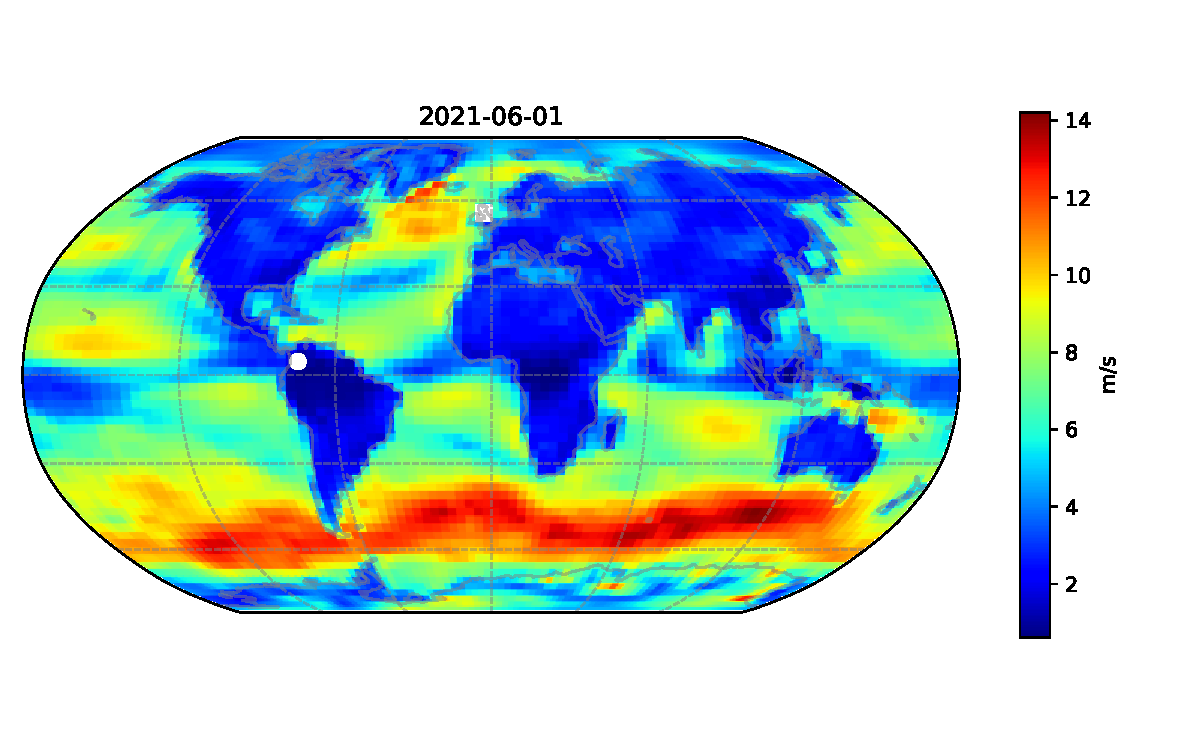
\includegraphics[width=\textwidth]{U10_example}
		\caption{U10 as at June 2021.}
		\label{fig:wind_june}   
	\end{subfigure}             
	\begin{subfigure}[b]{0.45\textwidth}
		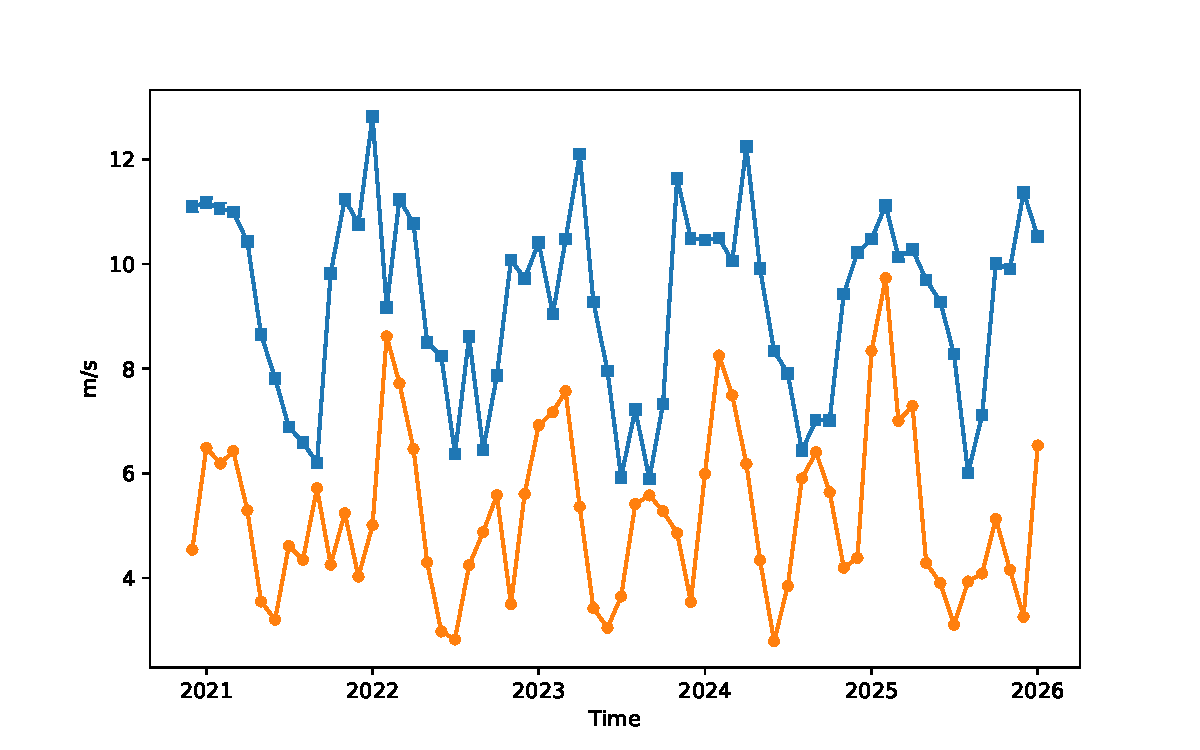
\includegraphics[width=\textwidth]{U10_example_temp}
		\caption{U10 over time.}
		\label{fig:wind_temp}
	\end{subfigure}             
	\caption[Overview of Wind variable]{Overview of the monthly average wind variable from CESM-LE ensemble member 1. Figure~\ref{fig:wind_june} highlights the spatial correlation present while Figure~\ref{fig:wind_temp} highlights the temporal correlation at two distinct locations; namely Colombia and the UK. The orange circle and blue square markers mark these respectively on Figure~\ref{fig:wind_temp} with the white markers highlighting their locations in Figure~\ref{fig:wind_june}.}
	\label{fig:wind_overview}
\end{figure}

\subsection{Replications}
For each variable discussed in Section~\ref{ssec:variables} the CESM-LE data provides $40$ replications; one from each ensemble member.
We have illustrated the spatial and temporal correlations in the four variables in the Figures~\ref{fig:precip_overview},~\ref{fig:pressure_overview},~\ref{fig:temp_overview}, and~\ref{fig:wind_overview} for a single simulation.
However we also have variability between replications and it is useful to illustrate this as it may provide insight into where we may expect difficulty in modelling.
It is important that any model developed for such data should be able to account for this variability in the data generating process.
Figure~\ref{fig:std_overview} displays a snap shot of the standard deviation of the respective variables in June 2021.

\begin{figure}[htbp!] 
	\centering
	\begin{subfigure}[b]{0.45\textwidth}
		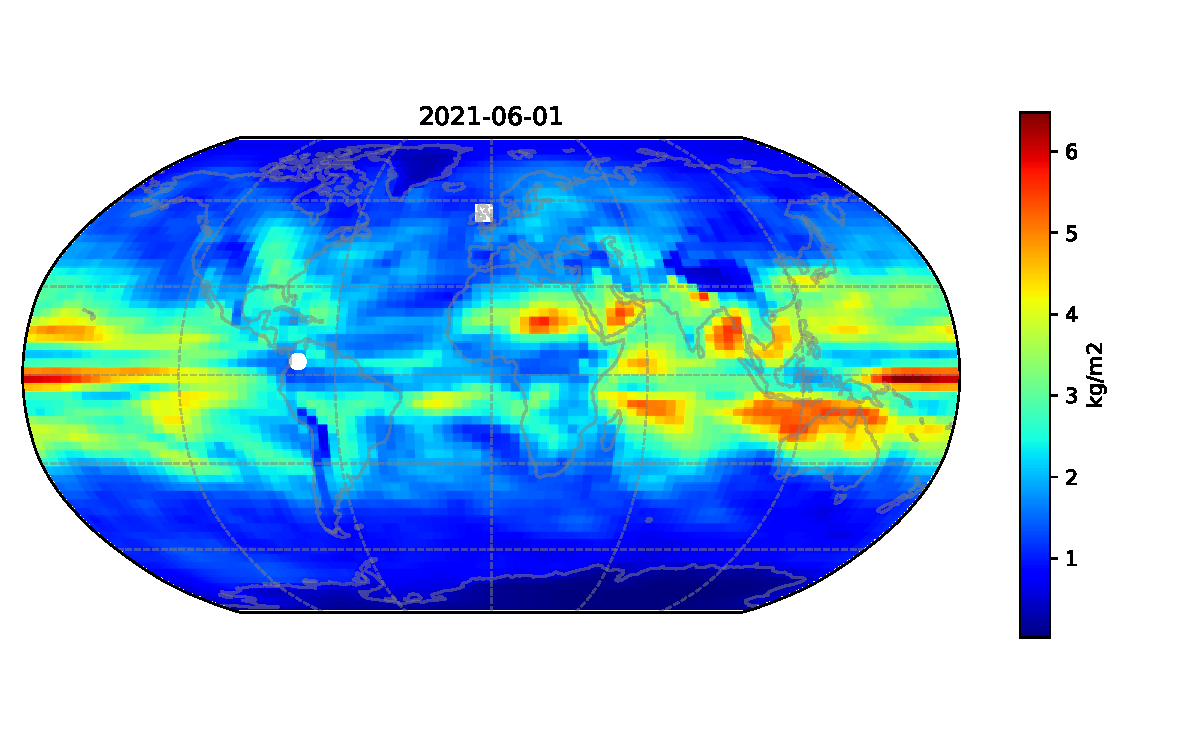
\includegraphics[width=\textwidth]{TMQ_std}
		\caption{TMQ.}
		\label{fig:std_precip_june}   
	\end{subfigure}             
	\begin{subfigure}[b]{0.45\textwidth}
		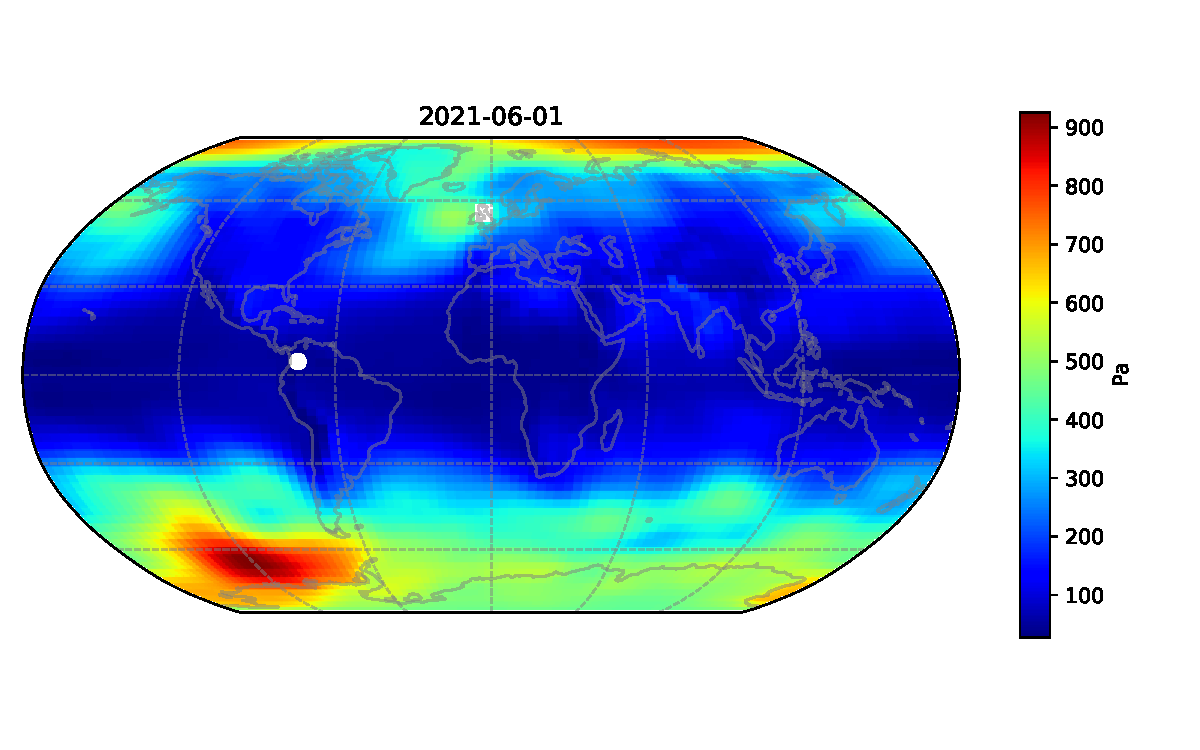
\includegraphics[width=\textwidth]{PS_std}
		\caption{PS.}
		\label{fig:std_pressure_june}
	\end{subfigure}             
	\hfill
		\begin{subfigure}[b]{0.45\textwidth}
		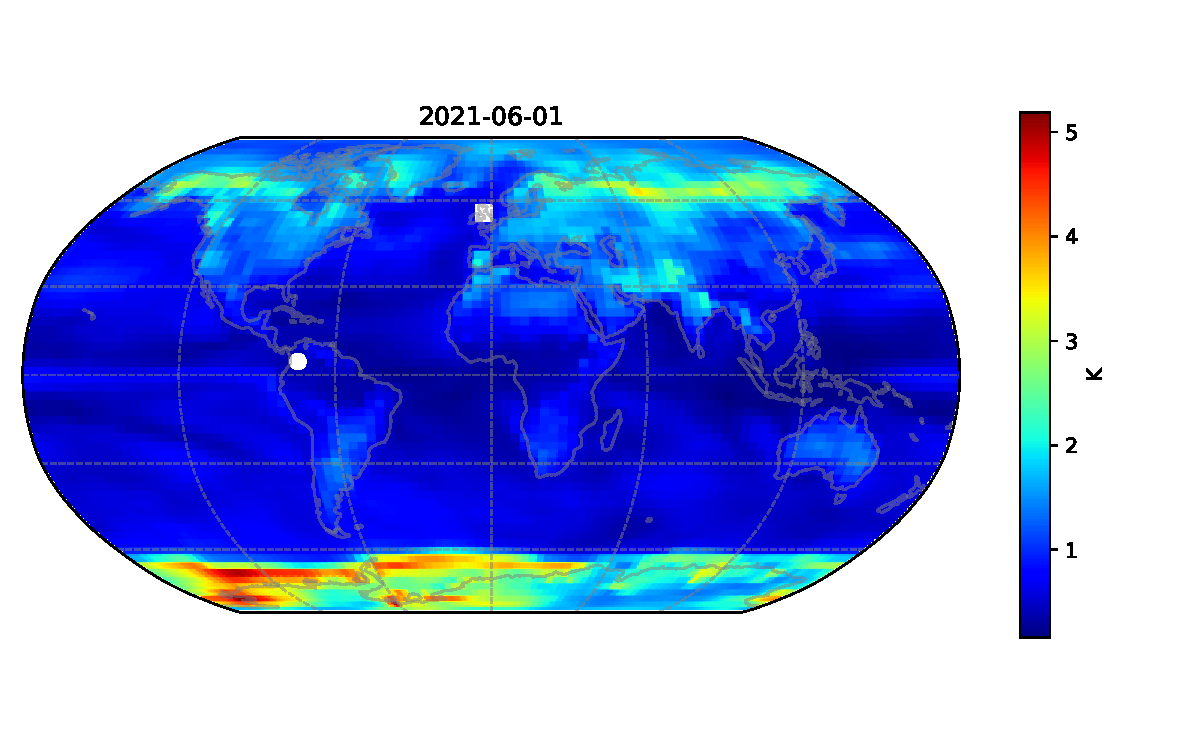
\includegraphics[width=\textwidth]{TREFHT_std}
		\caption{TREFHT.}
		\label{fig:std_temp_june}   
	\end{subfigure}             
	\begin{subfigure}[b]{0.45\textwidth}
		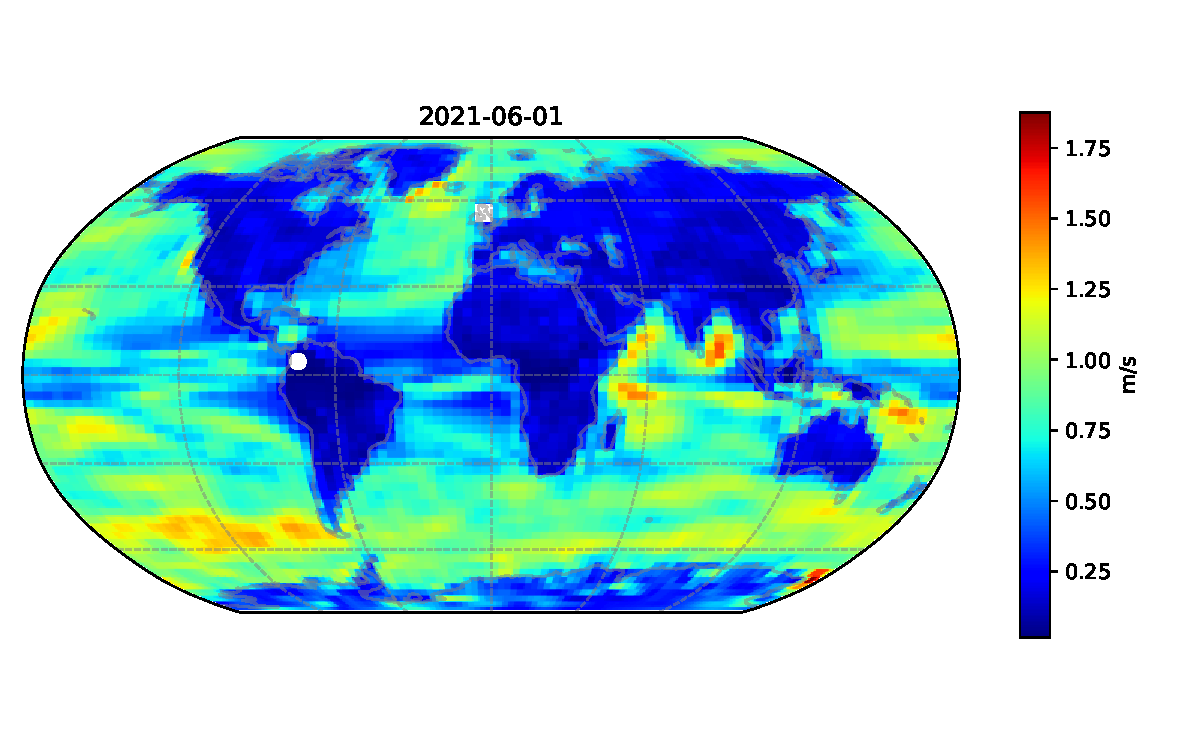
\includegraphics[width=\textwidth]{U10_std}
		\caption{U10.}
		\label{fig:std_wind_june}
	\end{subfigure}             
	\caption[Spatial overview of variability of Precipitation, Pressure, Temperature, and Wind speed.]{ Standard deviation of the four variables considered at June 2021 for the $40$ replications present in the CESM-LE data set. The locations of the UK and Colombia are shown by the white square and circle markers respectively. These points are used as examples in Figure~\ref{fig:std_overview_temp}. }
	\label{fig:std_overview}
\end{figure}

Figure~\ref{fig:std_overview} gives an indication of how drastically each simulation differs for each variable.
We would like to propose a model that can accommodate all the different scenarios presented in the various replications. 
Thus our model must be able to adapt to the regions of high standard deviation. 
From Figure~\ref{fig:std_precip_june} we can see that each simulation varies significantly in the tropics, but mostly around Indonesia.
As such we might be particularly interested in our model performance in this area for the precipitation variable.
For the pressure variable there is an increase in standard deviation for the poles and particularly to the south west of Antarctica, see Figure\ref{fig:std_pressure_june}.
There is a similar result for the temperature variable in Figure~\ref{fig:std_temp_june}.
Therefore we will be interested in model performance in this area for these variables.
The wind speed variable has many more localised areas with high variance from replications.
For example, the localised high variance of the coast of India and eastern Africa.  
These may pose a significant challenge to accommodate in a model for this variable.

Similar to the spatial variability in replications we can consider the variability over time.
Figure~\ref{fig:std_overview_temp} highlights this variation over the $40$ replications from the CESM-LE data set. 

\begin{figure}[htbp!] 
	\centering
	\begin{subfigure}[b]{0.45\textwidth}
		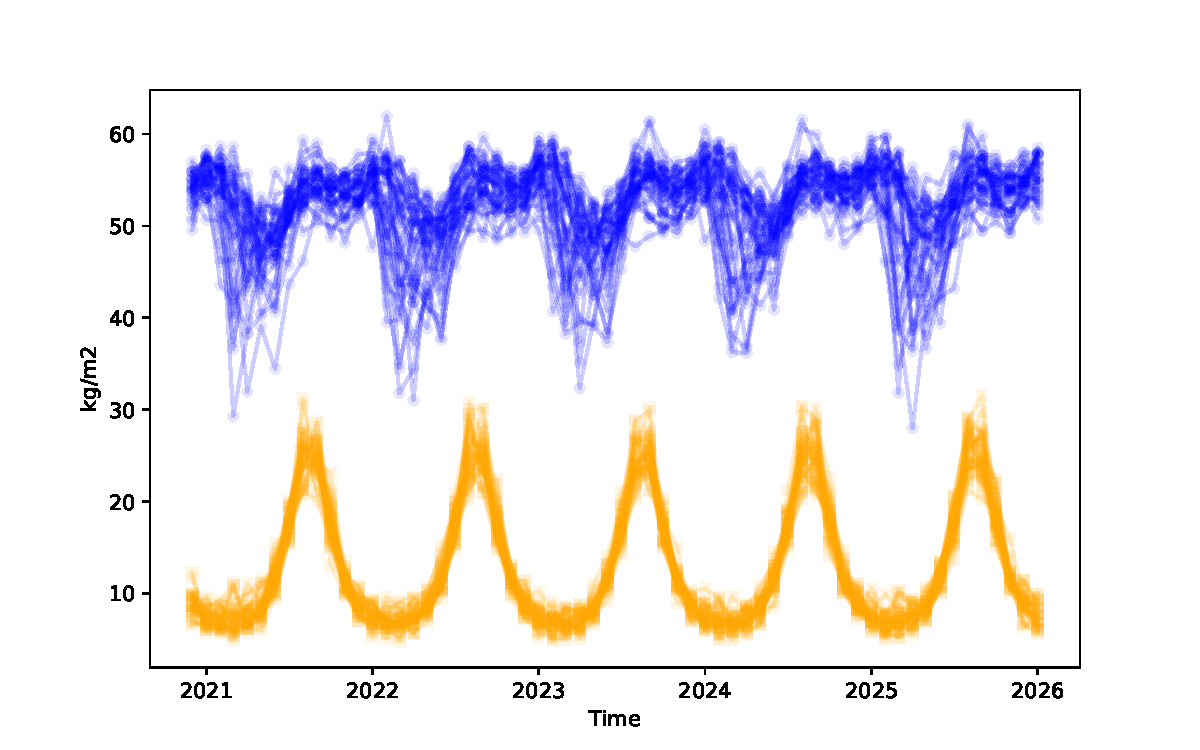
\includegraphics[width=\textwidth]{TMQ_std_temp}
		\caption{TMQ.}
		\label{fig:std_precip_temp}   
	\end{subfigure}             
	\begin{subfigure}[b]{0.45\textwidth}
		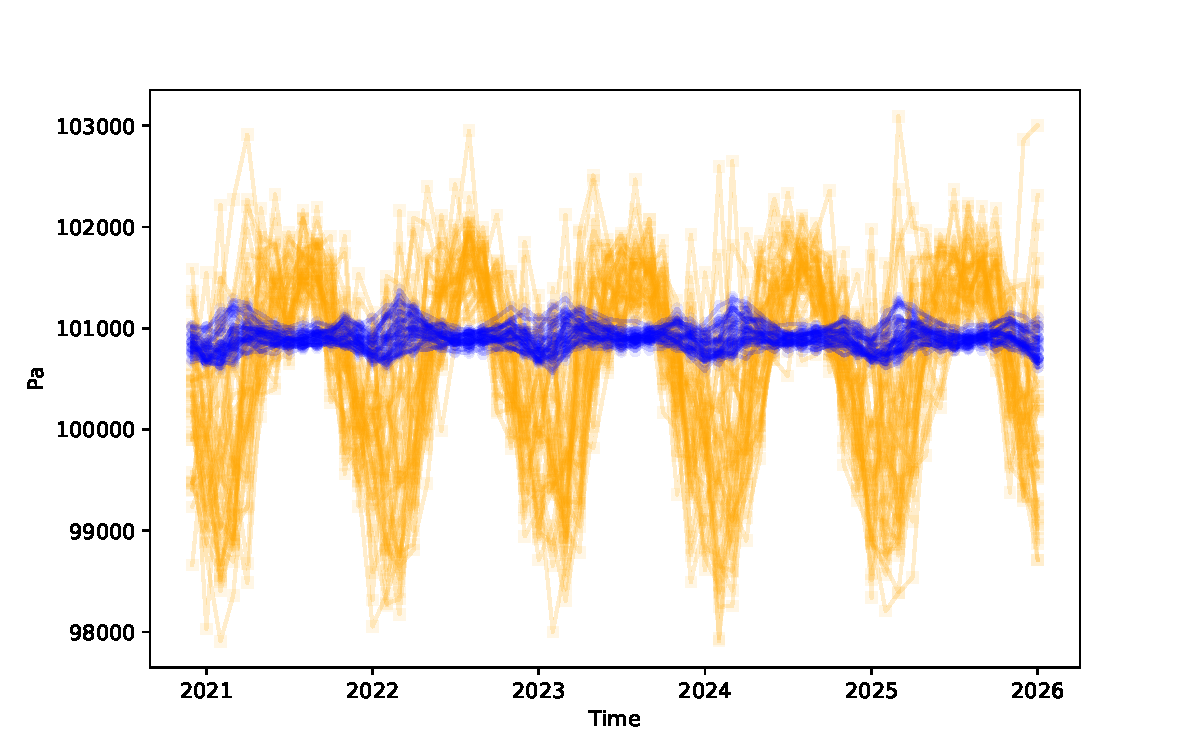
\includegraphics[width=\textwidth]{PS_std_temp}
		\caption{PS.}
		\label{fig:std_pressure_temp}
	\end{subfigure}             
	\hfill
	\begin{subfigure}[b]{0.45\textwidth}
		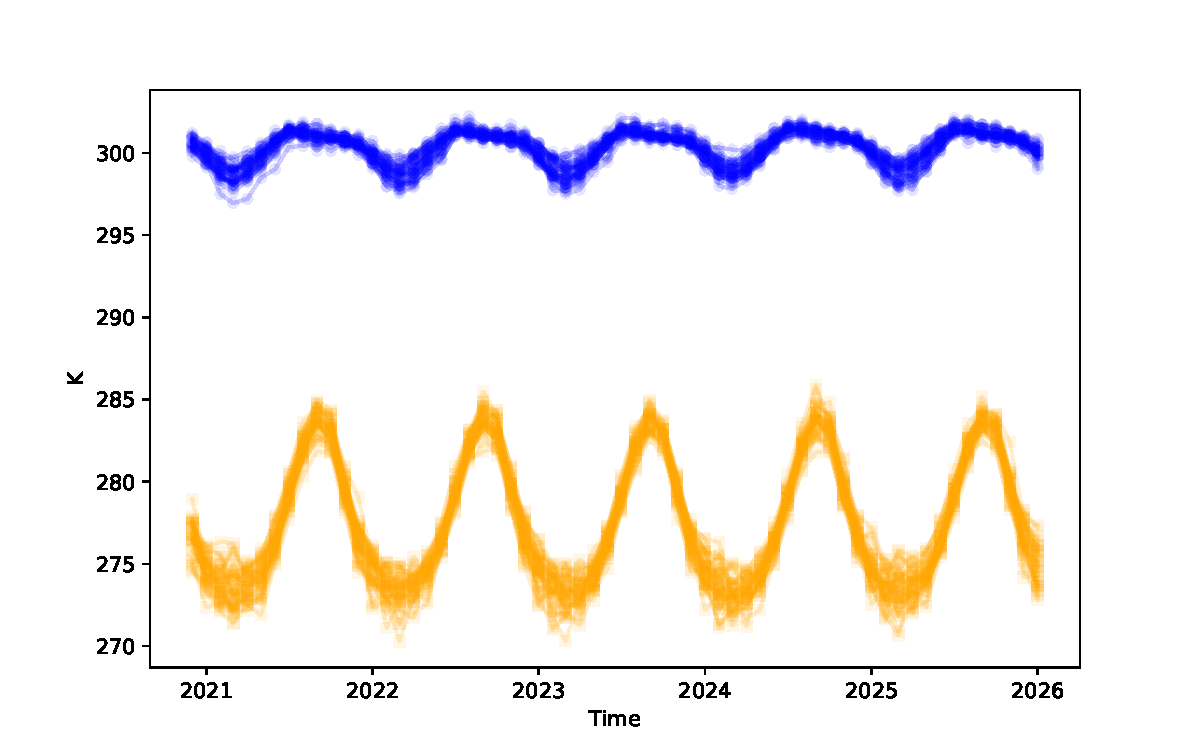
\includegraphics[width=\textwidth]{TREFHT_std_temp}
		\caption{TREFHT.}
		\label{fig:std_temp_temp}   
	\end{subfigure}             
	\begin{subfigure}[b]{0.45\textwidth}
		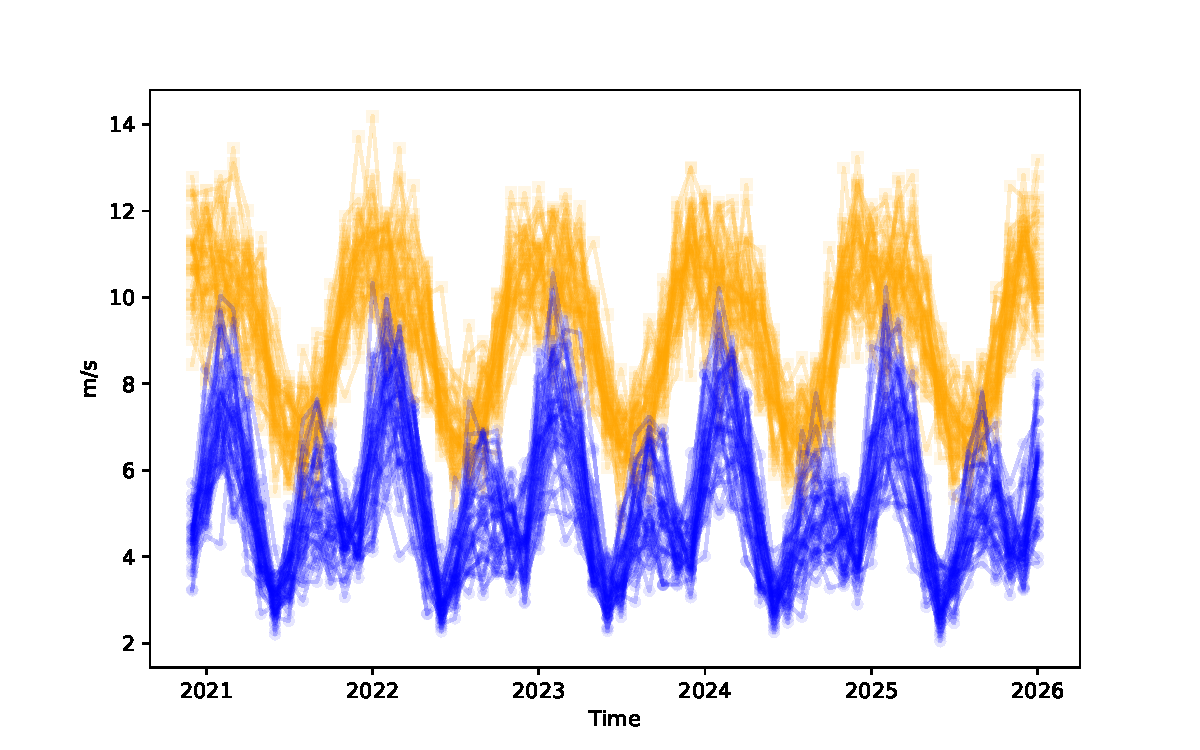
\includegraphics[width=\textwidth]{U10_std_temp}
		\caption{U10.}
		\label{fig:std_wind_temp}
	\end{subfigure}             
	\caption[Temporal overview of variability of Precipitation, Pressure, Temperature, and Wind speed.]{ Four variables over observation period December 2020 to January 2026 for the $40$ replications present in the CESM-LE data set at two locations; namely Colombia and UK. These are represented by the blue and orange colours respectively.}
	\label{fig:std_overview_temp}
\end{figure}

We can see clearly from Figure~\ref{fig:std_temp_temp} that the temperature variable function over time shows little variation between replications. 
However, variability does tend to increase in the troughs of these functions. 
Such a phenomena is more pronounced for the Colombia location. 
It may be interesting to assess performance of proposed models of the temperature variable with regard to this.
The precipitation functions vary differently for the Colombia and UK locations.
From the UK time series we see that although variability is high we can observe a periodic signal. 
It may be interesting to assess whether any model for this variable is able to pick up such a periodic signal, given that a single simulation may not show great periodicity.
Pressure similarly exhibits very different function variability between locations, with the Colombia functions showing large changes in pressure compared to the changes observed between replications at the UK location. 
Again this indicates that there is a clear spatial component to the process driving such replications. 

The above illustration of variability in replications gives an indication about the difficulties that any model must overcome to describe such variables and gives testament to the use of such a data set to test our proposed model for EO data.







%!TEX root = ../thesis.tex
%*******************************************************************************
%*********************************** Thrid Chapter *****************************
%*******************************************************************************

\chapter{Background Methodologies \label{cha:background}}  %Title of the Thrid Chapter

\nomenclature[a-GP]{$\mathcal{GP}\left(m(\cdot), k(\cdot, \cdot)\right)$}{Gaussian Process with mean function $m(\cdot)$ and covariance function $k(\cdot, \cdot)$}

\ifpdf
    \graphicspath{{Chapter3/Figs/Raster/}{Chapter3/Figs/PDF/}{Chapter3/Figs/}}
\else
    \graphicspath{{Chapter3/Figs/Vector/}{Chapter3/Figs/}}
\fi

In the following chapter we consider the various statistical methodologies  upon which we build our CPACE model.
This chapter is roughly structured so that we first focus on FDA techniques which are applicable, followed by smoothing methodologies which are use in the FDA techniques. 
Finally we discuss the multivariate techniques that are used in the CPACE model. 

\section{Functional principal components analysis \label{sec:fpca}}
A commonly used technique in multivariate statistics is that of Principal Components Analysis (PCA), \citep{wold_principal_1987}. 
The use of such a technique to find dominant directions of variation helps achieve dimensionality reduction and offers a parsimonious way to view data which is driven by the data themselves.
The equivalent technique when the data are functional in nature is known as Functional Principal Components Analysis (FPCA).
The basic concepts of which were studied in the mid twentieth century.
The work of \citeauthor{karhunen_zur_1946} and independently \citeauthor{loeve_fonctions_1946} paved the basic foundations of the technique in the FDA literature, \citep{karhunen_zur_1946, loeve_fonctions_1946}.
The FPCA technique essentially stems from representing the random function $\mathcal{X}(t)$ as an infinite linear combination of orthogonal functions.
Such a representation is now known as the Karhunen-Lo\`{e}ve theorem after its discoverers.

\subsection{Formulation}
The formulation of FPCA begins by assuming that $\mathcal{X}(t)$, $t \in \mathcal{T}$ is a square integrable stochastic process over some domain $\mathcal{T}$.
Let the mean and the covariance of the stochastic process $\mathcal{X}$ be denoted by $\mu(t)$ and $G\left(s, t\right)$ respectively, where:
\begin{align}
	\mu(t) &= \E \left(\mathcal{X}(t)\right) \label{eqn:mean_fn}\\
	G\left(s, t\right) &= \text{Cov}\left(\mathcal{X}(s),  \mathcal{X}(t)\right) \label{eqn:cov_fn}
\end{align}

Associated with the covariance surface $G\left(s, t\right)$ we have the linear operator $T_G$ defined by:
\begin{align}
	T_G &: L^2\left(\mathcal{T}\right) \to L^2\left(\mathcal{T}\right) \\
	T_G&:  f \mapsto T_G f = \int_{\mathcal{T}} G\left(s, \cdot \right) f(s) ds \label{eqn:t_op}
\end{align}

As $T_G$ is a linear operator we can consider its eigenvalues and eigenfunctions which we will denote by $\lambda_k$ and $\phi_k$ respectively (following convention set out in \citep{yao_functional_2005}) for $k=1,2,\cdots,$.
These are defined as the solutions to the Fredholm integral equations of the second kind: 

\begin{equation}\label{eqn:fredholm}
	\langle G(\cdot, t), \phi_k \rangle = \lambda_k \phi_k(t)
\end{equation}

where $\langle f, g \rangle = \int_{\mathcal{T}} f(s) g(s) ds$ is the inner product in the space $L^2(\mathcal{T})$. 
Then by the Karhunen-Lo\`{e}ve theorem one can express the centred process through the eigenvalues and eigenfunctions of the linear operator associated to the covariance surface.
That is:
\begin{equation}\label{eqn:fpca}
	\mathcal{X}(t) - \mu(t) = \sum_{k=1}^{\infty}\xi_k \phi_k(t)
\end{equation}
where $\xi_k$ is the $k^\text{th}$ principal component associated to the eigenfunction $\phi_k$.
The Karhunen-Lo\`{e}ve theorem assures us this $L^2$ convergence is uniform in $t$.
The principal components are given by the following: 
\begin{equation}\label{eqn:principal_comp}
	\xi_k= \langle \mathcal{X} - \mu, \phi_k \rangle 
\end{equation}

Further to this decomposition the Karhunen-Lo\`{e}ve theorem means we have that the principal components are independent from each other, centred and have variance equal to their associated eigenvalue.
That is:
\begin{align}
	\E\left(\xi_k\right) &= 0 \\
	\text{Var}\left(\xi_k\right) &= \lambda_k \\
	\E\left(\xi_k \xi_l\right) &= 0,~\text{for}~ k \ne l \label{eqn:principal_comp_uncorr}
\end{align}

\subsection{Interpretation}
As with the multivariate principal components analysis the interpretation of the eigenvectors is often useful in exploratory analysis of data.
The functional principal components analysis is of a similar form to the multivariate case and as such the same interpretation of the eigenfunctions is often employed.
As such the first eigenfunction $\phi_1(t)$ encapsulates the dominant mode of variation in $\mathcal{X}(t)$ by construction since:
\begin{equation}\label{eqn:first_comp}
	\phi_1 = \argmax_{\lVert \phi \rVert=1} \text{Var}\left( \langle  \mathcal{X} - \mu, \phi \rangle  \right)
\end{equation}
Similarly, the $k^\text{th}$ eigenfunction is the dominant mode of variation which is orthogonal to the preceding $k-1$ components.
As exploring the first few eigenfunctions often gives a parsimonious way to view the variation in the data.
Alike PCA it is often that the modes structure of the eigenfunctions replicates some observed physical process as such the FPCA decomposition is often used widely as a tool for data exploration. 

In addition to this we can use the fact that subsequent eigenfunctions capture less and less variation of the data as a form of dimensionality reduction, alike PCA.
In this sense we can consider truncating the full representation given in Equation~\eqref{eqn:fpca} to the $K$ leading eigenfunctions which gives an approximation to the full process which we will denote by $\mathcal{X}^K(t)$ where:
\begin{equation}\label{eqn:fpca_trun}
	\mathcal{X}^K(t)  =   \mu(t) + \sum_{k=1}^{K}\xi_k \phi_k(t)
\end{equation}
The approximation of $\mathcal{X}$ by $\mathcal{X}^K$ converges by:
\begin{equation}\label{eqn:fpca_trun_conv}
	\E \left( \langle  \mathcal{X} - \mathcal{X}^K, \mathcal{X} - \mathcal{X}^K \rangle \right)  =   \sum_{k > K}^{\infty} \lambda_k \to 0~\text{as}~K \to \infty
\end{equation}

As such using the leading principal components for reconstruction has the effect of capturing the main modes of variation of the data and ignoring smaller modes of variation.
Choosing the number of principal components is then up to the practitioner as in multivariate PCA, \citep{wold_principal_1987}.
 \citeauthor{ramsay_functional_2010} discuss in length the comparison of PCA to FPCA including commentary on the optimal choice of number of principal components, \cite[Chapter~8]{ramsay_functional_2010}.
 The practical implementation of FPCA involves then estimating various components.
 In particular estimation of;  the mean function $\mu(t)$, the covariance surface $G\left(s,t \right)$, the $K$ eigenfunctions and eigenvalues $\phi_k(t)$, $\lambda_k$ respectively, and the principal components $\xi_k$ for each realisation of the process $\mathcal{X}$ we observe.

\section{Principal analysis through conditional expectation \label{sec:pace}}
Assuming for now we have a sufficient method for estimating the mean  and covariance surfaces which we will denote by $\hat{\mu}(t)$ and $\hat{G}\left(s, t \right)$.
We discuss in more detail the estimation of these components in Section~\ref{sec:splines}.
Prior to the introduction of the Principal Analysis through Conditional Expectation (PACE) methodology in \citep{yao_functional_2005} FPCA decomposition was restricted due to the need for approximating the integrals in Equations~\eqref{eqn:principal_comp}.
As such it was often a requirement that the functional data were observed on a dense regular grid which meant that the principal components could be reliably estimated though some numerical integration scheme, \citep[Chapter~8]{ramsay_functional_2010}.
This very much restricted the application of the FPCA technique, however \citeauthor{yao_functional_2005} introduced the PACE method for over coming such an obstacle using conditional expectations for sparsely observed functional data.
In addition to this at the same time the technique accommodates for observation error. 

Traditionally Equation~\eqref{eqn:principal_comp} used for estimating the principal component scores for the $i^\text{th}$ realisation is approximated through sums.
Substituting $y_{ij}$ for $\mathcal{X}(t_{ij})$, $\hat{\mu}(t_{ij})$ for $\mu(t_{ij})$, and $hat{\phi}_k(t_{ij})$ for  $\phi_k(t_{ij})$ we obtain the estimate $\xi_i^{S} = \sum_1^{J_i}\left(y_{ij} - \hat{\mu}(t_{ij})\right)\hat{\phi}_k(t_{ij})\left(t_{ij} - t_{i(j-1)}\right)$, \citep{yao_functional_2005}.
Where $y_{ij}$ is as described in Equation~\eqref{eqn:fd_temporal} and setting $t_{i0}=0$.
However such an estimate breaks for the case that observations are sparse. Similarly such an approximation will be biased when the error processes from Equation~\eqref{eqn:fd_temporal}, $\varepsilon_{ij}$, is non-zero.
\citeauthor{yao_functional_2005} overcomes this by first assuming that the model is as follows:

\begin{align}
	y_{ij} &= \chi_{i} + \varepsilon_{ij} \\
	&= \mu(t_{ij}) + \sum_{k=1}^{\infty} \xi_{ik} \phi_k(t_{ij}) + \varepsilon_{ij} \label{eqn:fd_temporal_fpca}
\end{align}

with $\varepsilon_{ij}$ being jointly Gaussian with $\xi_{ik}$.
We also require the noise process satisfies:
\begin{align}
	\E\left(\varepsilon_{ij}\right) &= 0 \\
	\text{Var}\left( \varepsilon_{ij} \right) &= \sigma_\varepsilon^2
\end{align}

In addition to this the number of measurements of the $i^\text{th}$ subject is considered random which reflect sparse functional data.
Such a description follows naturally from our dataset description given in Equation~\eqref{eqn:fd_temporal} by using the FPCA decomposition structure of $\mathcal{X}$ as discussed in Section~\ref{sec:fpca}.
Following \citep{yao_functional_2005} we define the subsequent vector notations:
\begin{align}
	\vesub{Y}{i} &= \left(y_{i1}, y_{i2}, \cdots, y_{iJ_i}\right)^\top \label{eqn:yvec}\\
	\vesub{\phi}{ik} &= \left(\phi_{k}(t_{i1}), \phi_{k}(t_{i2}), \cdots, \phi_k(t_{iJ_i}) \right)^\top \label{eqn:phivec} \\
	\vesub{\mu}{i} &= \left(\mu(t_{i1}), \mu(t_{i2}), \cdots, \mu(t_{iJ_i})\right)^\top \label{eqn:muvec}\\
	\vesub{t}{i} &= \left( t_{i1}, t_{i2}, \cdots, t_{iJ_i} \right)^\top \label{eqn:tvec}
\end{align}
With such a model and assumptions, as stated in \citep{yao_functional_2005}, the best prediction of the principal component scores for the $i^\text{th}$  subject is given by:
\begin{equation}\label{eqn:fpc_best}
	\tilde{\xi}_{ik} = \E\left(\xi_{ik} | \vesub{Y}{i}, \vesub{t}{i} \right) = \lambda_k \vess{\phi}{ik}{\top} \vess{\Sigma}{\vesub{Y}{i}}{-1} \left( \vesub{Y}{i} - \vesub{\mu}{i} \right)
\end{equation}
where $\vesub{\Sigma}{\vesub{Y}{i}} = \text{Cov}\left(\vesub{Y}{i}, \vesub{Y}{i} \right)$.
The estimate for the principal component score can then be found by substituting in estimates for the various components in Equation~\eqref{eqn:fpc_best}.
That is:
\begin{equation}\label{eqn:fpc_est}
	\hat{\xi}_{ik}= \hat{\E}\left(\xi_{ik} | \vesub{Y}{i}, \vesub{t}{i} \right) = \hat\lambda_k \hvess{\phi}{ik}{\top} \hvess{\Sigma}{\vesub{Y}{i}}{-1} \left( \vesub{Y}{i} - \hvesub{\mu}{i} \right)
\end{equation}
The covariance matrix $\hvesub{\Sigma}{\vesub{Y}{i}}$ is formed with $\left(l, m\right)^\text{th}$ element:
\begin{equation}\label{eqn:sig_cov}
	\left[\hvesub{\Sigma}{\vesub{Y}{i}}\right]_{lm} = \hat{G}(t_{il}, t_{im}) + \hat{\sigma}_\varepsilon^2 \delta_{lm}
\end{equation}
where $\hat{\sigma}_\varepsilon^2$ is the estimated variance of the noise process.
The estimation method for this is discussed in Section~\ref{sec:splines}.
\citeauthor{yao_functional_2005} also provide asymptotic properties of such an estimator  along with asymptotic confidence bands where the mean and covariance surfaces are estimated with local linear smoothers, \citep{fan_study_1996}.

The conditional expectation technique describe above from \citep{yao_functional_2005} alleviates the issue of poor integral approximation from sparsely observed data when the estimated covariance surface is a relatively good fit to the true covariance surface.
This is a somewhat better condition as it allows one to pool data from different observed subjects to estimate such a surface and thus the requirement of dense data per subject is relaxed to having dense data from the collection over all subjects.
We discuss a particular method for estimating such surfaces in Section~\ref{sec:splines}.

\section{Penalised regression splines \label{sec:splines}}
 Smoothing models underpin much of FDA.
 FDA uses the smoothness of observations over a continuous domain to help inform and model observed data.
 Typically, as described in Section~\ref{sec:fr}, data is only observed discretely.
 Therefore with most FDA methodology there must be a conversion from discretely observed data and the continuous functional variable that generates it.
 This is particularly the case for our EO data since we have discrete observations specified by our data model given in Equation~\eqref{eqn:observed_data} which we assume is generated by observations of continuous functions or surfaces given by our models in Equation~\eqref{eqn:fd_temporal}.
 As such many models for obtaining such a smooth of the data have been studied, such as kernel smoothing, polynomial regression, and local linear smoothing, \citep[Chapter~4]{ramsay_functional_2010}. 
 In this section we consider the well studied technique of obtaining smooths of discrete data through penalised spline regression.
 We will use such a method to estimate the mean and covariance surfaces present in PACE methodology described in Section~\ref{sec:pace}. 
 
 \subsection{Basis Splines  \label{ssec:basis_splines}}
 One of the components of a penalised spline regression is the basis functions used in the regression.
 As the name suggests spline regression uses spline functions as the regression basis.
 Spline functions of order $d$,  which are well documented in the monograph of \citeauthor{de_boor_practical_2001}, is a piecewise polynomial function of degree $d-1$, \cite{de_boor_practical_2001}. In the case of a spline function of order $d$, $S: \mathcal{T} \to \mathbb{R}$, over a univariate domain $\mathcal{T} = \left[a, b\right] \subset \mathbb{R}$ we have: 
 \begin{equation}
 	S: t \mapsto S(t) = \begin{cases}
 		P_0(t)~\text{if}~ \tau_0 < t  \leq \tau_1,\\
 		P_1(t)~\text{if}~ \tau_1 < t  \leq \tau_2,\\
 		\vdots \\
 		P_{m-1}(t)~\text{if}~ \tau_{m-1} < t  \leq \tau_m,\\
 	\end{cases}
 \end{equation}
where $P_i: \left[\tau_i, \tau_{i+1}\right] \to \mathbb{R}$ are polynomial functions of degree $d-1$.
The vector of points $\ve{\tau} = \left(\tau_0, \tau_1, \cdots, \tau_m \right)$ is known as the knot vector for the spline and must satisfy $a=\tau_0 < \tau_1 < \cdots < \tau_m = b$.
 By specifying that the piecewise polynomials must share the same derivative order up to a degree we can ensure continuity of relative smoothness over the knot points and the whole spline function.
 We specify the continuity at each point in our knot vector by the continuity vector $\ve{r}=\left( r_0,\cdots, r_m \right)^\top$ where $r_i$ specifies that $P_i$ and $P_{i+1}$ share common derivative values at point $\tau_i$ for derivatives up to order $r_i$.
 The spline type can be specified completely by specifying the knot locations and the continuity vector, \citep{de_boor_practical_2001}.
 In fact one can extend our definition of the knot vector to incorporate both the knot and continuity vector into one vector, known as the extended knot vector, which will completely specify the spline type.
 We define the extended knot vector as the vector of knot points which repeats the $i^\text{th}$ knot vector exactly $n - r_i$ times. That is:
\begin{equation*}
	(\tau_0,\cdots,\tau_0, \tau_1, \cdots, \tau_1 ,\cdots, \tau_{m-1},\cdots, \tau_{m-1}, \tau_m \cdots, \tau_m)
\end{equation*}
We denote the spline functions of order $d$ with extended knot vector by $S_{d, \ve{\tau}}$. 

The Basis splines are more commonly referred to as B-splines, \citep{knott_interpolating_2000}.
B-splines are basis functions for splines of the same order defined over the same knots.
They are typically defined recursively, \citep{knott_interpolating_2000, de_boor_practical_2001}.
The classic algorithm for the recursive construction is known as the Cox-de Boor recursion formula, \citep{de_boor_practical_2001}, and is given as follows.
Given a knot vector $(\tau_0,\cdots,\tau_0, \tau_1,\cdots,  \tau_1, \cdots, \tau_{m-1},\cdots, \tau_{m-1}, \tau_m,\cdots, \tau_m)^\top$ the B-spline of order $1$ is given by:
\begin{equation}	\label{eqn:bspline1}
	B_{i, 1}\left( t \right) = \begin{cases} 1,~\text{for}~\tau_i \le t < \tau_{i+1} \\ 0,~\text{otherwise.} \end{cases}
\end{equation}

The higher order B-splines are defined by recursion as:
\begin{equation}\label{eqn:bspline_high}
	B_{i, q+1}(t) = w_{i, p}(t) B_{i, q}(t) + \left[ 1 - w_{i+1, q}(t) \right]B_{i+1, q}(t)
\end{equation}
where $w_{i, q}$ is a weighting for the $i^\text{th}$ B-spline of order $d$ given by:
\begin{equation}
	w_{i, q}(t) = \begin{cases} \frac{x-\tau_i}{\tau_{i+q} - \tau_i} ,~\text{for}~\tau_{i+q} \ne \tau_i \\ 0,~\text{otherwise.} \end{cases}
	\label{eqn:weighting}
\end{equation}
A B-spline basis system of size $Q$ can then be considered by choosing the extended knot vector $\ve{\tau}$ and specifying the order, $d$, of the B-spline functions, and is given by the collection:
\begin{equation}
	\{ B_{d, q}^{\ve{\tau}}(t)\}_{q=1}^{Q}
	\label{eqn:bspline_basis}
\end{equation}
where $Q$ is the number of basis functions to use in the system, $\ve{\tau}$ is the extended knot vector, and $B_{d, q}^{\ve{\tau}}$ is the $q^\text{th}$ B-spline of order $d$ defined by Equation~\eqref{eqn:bspline_high} for our knot vector $\ve{\tau}$.
Figure~\ref{fig:bspline_basis} shows the first $7$ B-spline functions of order 4 with equally spaced knots over the domain $\left[ 0, 1 \right]$.

 \begin{figure}[htbp!] 
	\centering    
	
\includegraphics[width=1.0\textwidth]{Example_image}
	\caption[Example  B-spline functions of order 4]{First seven B-spline functions of order four with equally spaced interior knots over the domain $\left[ 0, 1 \right]$. The vertical dotted lines indicate the knot positions.}
	\label{fig:bspline_basis}
\end{figure}

\subsection{Regression splines \label{ssec:spline_reg}}
As discussed in Section~\ref{sec:pace} the PACE methodology requires estimation of both the mean function, $\mu(t)$, and covariance surface $G\left(s, t\right)$. 
Estimating such functions is a problem due to their infinite dimensional nature.
A well studied and effective method for representing such functions is the use of a basis function expansion,  \cite{ramsay_functional_2010}.
That is representing the target surface using a linear combination of known basis functions.
In this work we will utilise the B-spline basis function as discussed in Section\ref{ssec:basis_splines}.
The B-spline system is exceptionally popular due to its ease of computation and ability to reconstruct many surfaces, \citep{de_boor_practical_2001}.
Such ease of computation makes it feasible to not only create large basis systems but also alleviates many fitting procedures as we can re-evaluate the basis system at various points with ease.
Such properties are very useful when using such a basis for regression models. 
Common basis systems include the Fourier, Monomial, and Polynomial basis systems, \cite{ramsay_functional_2010}.
In the following we present the approach for estimating an arbitrary realisation of our functional random variable $\chi(t)_i$ over domain $\mathcal{T}$ and discuss how we extend the same concept to a two dimensional surface over $\mathcal{T} \times \mathcal{T}$ in Section\ref{sssec:spline_ext}.

As such we assume that our function  can be represented using an order $d$ B-spline basis system with knot vector $\ve{\tau}$: 

\begin{align}
	\chi(t)_i &= \sum_{q=1}^Q c_q B_{d, q}^{\ve{\tau}}(t) \\
	&= \vesup{c}{\transpose} \vess{B}{d}{\ve{\tau}}(t) \label{eqn:basis_expansion}\\
\end{align}

where $\ve{c}=\left( c_1,\cdots, c_K \right)^\transpose$, $\vess{B}{d}{\ve{\tau}}(t) = \transpose{\left( B_{d, 1}^{\ve{\tau}}(t), B_{d, 2}^{\ve{\tau}}(t), \cdots, B_{d, Q}^{\ve{\tau}}(t) \right)}$, and $Q$ is the dimension of the expansion.
An example of such a basis expansion is given in Figure~\ref{fig:basis_expansion}.
From this we can clearly see how the function $\chi_i$ is broken down into a finitely many constituent parts of scaled known basis functions.
If such basis functions have nice properties such as simplicity to compute then such a representation for $f$ given by Equation~\eqref{eqn:basis_expansion} can be extremely useful since most problems can be reduced to problems involving the finite dimensional vector $\ve{c} \in \mathbb{R}^Q$. 

\begin{figure}[htbp!] 
	\centering    
	
\includegraphics[width=1.0\textwidth]{Example_image}
	\caption[Example B-spline basis expansion]{Example B-spline basis expansion of known function with basis functions shown for clarity.}
	\label{fig:basis_expansion}
\end{figure}

Our representation of $\chi_i$ using a basis system then becomes the problem of choosing the coefficients $\vesup{c}{\transpose}$ using only our set of observations of $\vesub{Y}{i}$ which are observed with error.
The most common method for fitting a basis system to discretely observed data is by choosing the coefficients of the expansion $c_q$ given in Equation~\ref{eqn:basis_expansion} by minimising the criterion:
\begin{equation}
	\text{SSE}_{\vesub{Y}{i}}\left( \ve{c}\right) = \lVert \vesub{Y}{i} - \ve{B}\vesup{c}{\transpose} \rVert^2
	\label{eqn:sse}
\end{equation}
where $\ve{B} = \left( \vess{B}{d}{\ve{\tau}}(t_{i1}),\vess{B}{d}{\ve{\tau}}(t_{i2}),\cdots, \vess{B}{d}{\ve{\tau}}(t_{iJ_i}) \right)^\transpose$ is the $J_i \times Q$ matrix of the basis system evaluated at observed time points corresponding to the $J_i$ length observation vector $\vesub{Y}{i}$. Minimising such a criterion is given by, \cite{bjorck_numerical_1996}:
\begin{equation}
	\hat{\ve{c}} = \left( \vesup{B}{\transpose} \ve{B} \right)^{-1}\vesup{B}{\transpose}\vesub{Y}{i}
	\label{eqn:hatc}
\end{equation}

The simple least squares approximation is a well studied and standard approach. See \citep{bjorck_numerical_1996} for a through introduction to the concept. 
Such a methodology is often suitable for situations where our error process $\varepsilon(t)$ is a white noise process.
Such a process for the noise is often unrealistic; as such a simple adjustment to the least squares criterion in Equation~\ref{eqn:sse} can be used to allow for correlation among the observation errors: 
\begin{equation}
	\text{SSE}_{\vesub{Y}{i}, \ve{W}}(\ve{c}) = \lVert \ve{W}^\frac{1}{2}\left( \vesub{Y}{i} - \ve{B}\vesup{c}{\transpose} \right) \rVert^2
	\label{eqn:wsse}
\end{equation}
where $\ve{W}$ is a weighting matrix for the observations. Ideally the matrix will be the inverse of the variance-covariance matrix of the observations. Minimising the adjusted criterion is given by, \cite{bjorck_numerical_1996}:
\begin{equation}
	\hat{\ve{c}} = \left( \vesup{B}{\transpose} \ve{W} \ve{B} \right)^{-1}\vesup{B}{\transpose} \ve{W} \ve{y}
	\label{eqn:whatc}
\end{equation}
The estimate with least squares fitting can then be substituting $\hat{\ve{c}}$ for the $\ve{c}$ in Equation\ref{eqn:basis_expansion}, \citep{bjorck_numerical_1996}. That is:
\begin{equation}\label{eqn;hat_basis_expansion}
	\hat{\chi}_i(t) = \vesup{\hat{c}}{\transpose} \vess{B}{d}{\ve{\tau}}(t)
\end{equation}
The selection of the knot vector is well studied and the classical choice is to choose a knot vector where knots are located at the sampling points, \citep{de_boor_practical_2001}. 

An issue with the classical least squares fitting using a basis system expansion is the choice of number of basis functions, \cite{ramsay_functional_2010}.
Although we are constrained to choose $Q$ to be less than or equal to the number of observations, $J_i$, since more than $J_i$ basis functions would results in Equation~\ref{eqn:whatc} being ill defined as the matrix $\ve{B}$ cannot have linearly independent columns.
However, we still have the choice to choose $Q$ between $1$ and $J_i$.
Exactly which value for $Q$ to choose is unknown and results in the classical problem of bias variance trade off in the estimator.
A large number of basis functions reduces bias in the estimator $\hat{\chi}_i(t)$, but the variance of this estimator may be unacceptably high.
Similarity a lower number of basis functions will result in high bias of the estimator but low variance.
The bias-variance trade off is well studied and there is a vast literature on the methodology of choosing the number of basis functions, however there is no gold standard and often the choice is made in an ad hoc fashion, \citep{ramsay_functional_2010}. 
Such an issue motivates modifying the fitting criterion which determines $\ve{\hat{c}}$ in Equation~\eqref{eqn:whatc}.

\subsubsection{Penalties}
Ideally we want to penalise estimators which have high variance, that occur naturally when we have a large number of basis functions, but keep bias low.
The naive choice of just reducing the number of basis functions, known as regression splines, fails in this respect, \cite{ruppert_semiparametric_2003}.
One such approach to do this is to reduce the number of basis functions in conjunction with a penalty, known as penalised regression splines.
Such an approach was first used in \citep{osullivan_statistical_1986} who used such a formulation on ill posed inverse problems.
\cite{ruppert_semiparametric_2003} discuss various other spline smoothing techniques as well as the penalised regression splines.

Penalised regression spline models adjust the fitting criterion in Equation~\eqref{eqn:whatc} to:
\begin{equation}\label{eqn:plss}
	\text{PSSE}_{\vesub{Y}{i}, \ve{W}, \lambda}(\ve{c}) = \lVert \vesup{W}{\frac{1}{2}}\left( \vesub{Y}{i} - \ve{B}\ve{c} \right) \rVert^2 + \omega \vesup{c}{\transpose} \ve{P} \ve{c}
\end{equation}
where $\ve{P}$ is formed with $(l,m)^\text{th}$ element $\left[\ve{P}\right]_{lm} = \langle L\left(\vesub{B}{l}\right), L\left( \vesub{B}{m} \right) \rangle$ and $\omega$ is a parameter which controls the regularisation trade off.
$L$ is some linear differential operator.
Typically one chooses $L$ to be the required smoothness of the target function and examples include simple first or second derivatives, \cite{ruppert_semiparametric_2003}.

Analytically minimising the $\text{PSSE}$ criterion in Equation~\eqref{eqn:plss} can be found via:
\begin{equation}
	\hat{\ve{c}} = \left( \vesup{B}{\transpose} \ve{W} \ve{B} + \omega \ve{P} \right)^{-1}\vesup{B}{\transpose} \ve{W} \vesub{Y}{i}
	\label{eqn:phatc}
\end{equation}

Essentially such a penalisation term determines that there should be a trade off between the bias which corresponds to the first term in Equation~\eqref{eqn:plss} and the variance which is the second term.
This trade off is controlled by the regularisation parameter $\omega$.
The advantage of this method is that we can now let $Q$, our number of basis functions, be large without worrying of over fitting as the penalty term in Equation~\eqref{eqn:plss} will penalise functions with high variability in terms of the differential operator $L$.

The choice of differential operator is a well studied problem also. A common choice is the first or second order differential, denoted by  $D^1$ and  $D^2$ respectively, as this specifies a reasonable level of smoothness in the target function, \cite{ruppert_semiparametric_2003}. However, often more complex terms are used to facilitate known properties of the target functions, such a letting $L$ be the harmonic acceleration operator which forces a periodic form of the target functions.
More care must be taken when extending the linear differential operator to higher dimensions which is discussed in Section~\ref{sssec:spline_ext}.
Additionally, in the case of B-spline basis system these penalty matrices are typically evaluated using a form of numerical integration, \cite{ramsay_functional_2010}.

Considering a penalised for of regression splines moves our problem of selecting $Q$ to choosing our regularisation parameter, $\omega$.
Such a parameter influences the strictness with which we expect our target function to be smooth as defined by the operator $L$.
Choosing such a parameter is a problem that is present not only in spline smoothing but other penalised regression approaches, \citep{lukas_robust_2006}.
A popular method for choosing such a parameter is the Generalised Cross Validation (GCV).
GCV, introduced by \citeauthor{wahba_practical_1977},, is a well studied method which has good asymptotic properties as $J_i$, the number of observations tends to infinity, \citep{wahba_spline_1990, wahba_comparison_1985}.
GCV chooses $\lambda$ as the minimiser of the GCV criterion $V(\omega)$ which is given by:
\begin{equation}\label{eqn:gcv}
	V\left(\omega\right) = \frac{J_i^{-1} \lVert \left(\ve{I} - \ve{A} \right) \vesub{Y}{i} \rVert^2}{\left[ J_i^{-1} \text{tr}\left(\ve{I} - \ve{A}\right)\right]^2}
\end{equation}
where $\ve{A}$ is the influence matrix defined by:
\begin{equation}\label{eqn:inf}
	\ve{A} = \ve{B} \left( \vesup{B}{\transpose} \ve{W} \ve{B} + \omega \ve{P} \right)^{-1}\vesup{B}{\transpose} \ve{W}
\end{equation}
The GCV method can then be minimised for $\omega$ using a numerical minimisation routing.
For large $J_i$ it is known that the GCV criterion performs well in recovering a regularisation parameter which minimises variance while maintaining low bias in the reconstruction of the target function, \citep{wahba_comparison_1985}.
For the case of low $J_i$ the GCV method may not be reliable as such method to extend the GCV criterion have been considered.
The modified GCV criterion, which adds a further modifier to the denominator in Equation~\eqref{eqn:gcv} by multiplying the trace of the influence matrix by a factor, \citep{cummins_confidence_2001}.
The modified GCV approach effectively increases the cost associated with each effective parameter in the curve which reduces choosing $\omega$ which under smooths the data, \citep{cummins_confidence_2001}.
A similar but separate approach to adjusting the GCV is robust GCV, introduced by \citeauthor{lukas_robust_2006}, which uses a weighted sum of the GCV function with a term which penalises $\omega$ values that are close to zero, \citep{lukas_robust_2006}.
The performance of such methods are discussed in \citep{lukas_performance_2012}.

Choosing a basis system, a criterion to choose the regularisation parameter and a differential operator then fully specified the penalised regression spline approach.
In the case of one dimensional functions the procedure applies as above. As such we can estimate our mean function $\mu(t)$ through the use of a penalised spline regression where our observation points for the mean function are the pooled mean across subject of the union of observed time points for all curves.
However for multiple dimensions, particularly the case when we wish to smooth the covariance surface, we must make some adjustments to the penalty.
These are discussed in Section~\ref{sssec:spline_ext}.

\subsubsection{Extension to higher dimensions \label{sssec:spline_ext}}
There are two issues when extending the penalised regression spline to higher dimensions; extending the basis system and extending the penalty specification.
To alleviate the first we must specify a basis system which can cover multiple dimensions. In fact there are many such systems, \citep{wahba_spline_1990}.
One such popular approach when we have regular data for FDA is using a tensor product B-spline system, \citep{xiao_asymptotic_2020}.
Consider a two dimensional surface$\sigma \left(s, t\right)$ which we represent by the tensor product spline given by:
\begin{equation}\label{eqn:tensor_expansion}
	\sigma \left(s,t\right) = \sum_{1 \le q_1, q_2 \le \bar{Q}} c_{q_1, q_2} \vess{B}{d_1}{\vesub{\tau}{1}}(s)\vess{B}{d_2}{\vesub{\tau}{2}}(t)
\end{equation} 
where $\vess{B}{d_i}{\vesub{\tau}{i}}$ is the B-spline basis system for the $i^\text{th}$ dimension for $i=1,2$.
For notational simplicity we assume the dimension of each marginal basis system is the same, $\bar{Q}$ however this need not be the case.
$\ve{C} \in \mathbb{R}^{\bar{Q} \times \bar{Q}}$ is a coefficient matrix to be determined.
Equation~\eqref{eqn:tensor_expansion} can be written more succinctly using a Kronecker product as:
\begin{equation}\label{eqn:kron_expansion}
	\sigma\left(s,t\right) = \vesup{\bar{B}}{\transpose}\left(s, t\right) \text{Vec} \left(\ve{C}\right)
\end{equation}
where $ \ve{\bar{B}}\left(s, t\right) = \vess{B}{d_2}{\vesub{\tau}{2}}(t) \otimes \vess{B}{d_1}{\vesub{\tau}{1}}(s)$ and $\text{Vec}\left(\cdot\right)$ is an operator which stacks the columns of a matrix into a vector. We use the $\bar{\cdot}$ notation to make explicit that this basis is over multiple dimensions.

The same methods now follow as in the non penalised univariate case with this Kronecker basis system, \citep{xiao_asymptotic_2020}.
However, we must still adjust the penalty matrix in Equation~\eqref{eqn:phatc} to account for smoothness across multiple dimensions. 

Using the tensor product basis system as described above one might consider specifying that the smoothness of the surface in smooth in both dimensions.
Indeed, one such approach to extending the penalty specification which was introduced by \citeauthor{wood_low-rank_2006} is to consider setting penalties on the marginal basis separately and to combine them by a weighted sum, \cite{wood_low-rank_2006}.
Such an approach known as tensor product penalties is well studied in the linear generalised additive model setting, \cite{wood_generalized_2006}. 
A two dimensional penalty matrix $\bar{\ve{P}}$ may be described as follows: 
\begin{equation}\label{eqn:tensor_pen}
	    \bar{\ve{P}} = \omega_1 \ve{P}_1 \otimes \ve{I}_2 + \omega_2 \ve{I}_1 \otimes \ve{P}_2
\end{equation}
where $\vesub{P}{i}$ is marginal penalty over a single basis dimension as described in Equation~\eqref{eqn:plss}, $I_i$ is the identity matrix of dimension of the $i^\text{th}$ dimension basis, and $omega_i$ is the marginal regularisation parameter for $i=1,2$.
The properties of such a smoothness penalty are discussed in detail in \citep{wood_low-rank_2006} with the main points being such a penalty is both scale invariant and low rank. In addition \citep{wood_p-splines_2017} studies the use of such a penalty for the case of unevenly distributed data. The additional complication is we now have multiple smoothness parameters $\omega_i$, one for each dimension of the surface to be smoothed. In this case the GCV methodology can still be applied but now minimisation occurs with respect to the vector $\ve{\omega}$. Implementation details of such can be found in \cite{wood_generalized_2006}.

With an extension to multiple dimensions we can now use the above approach to estimate our covariance surface, denoted by $\hat{G}\left(s,t\right)$, for use in PACE methodology, \citep{yao_functional_2005}. The discrete observations for the covariance surface to be smoothed are gathered by pooling individual observed covariances from across subjects, which is discussed in detail in both \citep{yao_functional_2005, xiao_asymptotic_2020}. 
\citeauthor{xiao_asymptotic_2020} provides asymptotic properties of such an approach to the covariance surface of independent functional data which are on par to the asymptotic results of other smoothers used in \citep{yao_functional_2005} for the PACE methodology, \citep{xiao_asymptotic_2020}.

\section{Functional time series\label{sec:fts}}
As discussed in Section~\ref{sec:eo} EO data is often both spatially and temporally correlated.
This two types of correlation is often considered separately. 
An area in FDA which has considered a similar case where functional data is observed and observations are correlated is functional time series, \citep{aguilera_forecasting_1999}. Typically, functional observations are naturally indexed by some time of observation and correlation may occur between observations. Hence we may build up a time series of functional observations. Functional time series models are some of the first in the FDA literature to start to consider correlated functional observations.
Although they limit themselves to temporal correlation many of the ideas can be considered for extensions to higher dimension correlation and so we discuss a few of the more popular methodologies in this section.

We focus on a technique introduced by \citeauthor{hyndman_forecasting_2009} in \citep{hyndman_forecasting_2009} to forecast functional time series.
Such a method is of interest as it expands methodology on how to use existing forecasting techniques in a functional setting.
In particular \citep{hyndman_forecasting_2009} uses the FPCA decomposition described in Section~\ref{sec:fpca} to decompose functional observations and then uses independent forecasting of each principal component scores using standard multivariate techniques.

\citep{hyndman_robust_2007} suggests to assume the principal component scores, $\xi_{ik}$ follow independent univariate time series. Then, conditioning on the observed data $Y$ given in Equation~\eqref{eqn:observed_data} and the set of principal components $\ve{\phi}(t) = \left(\phi_1(t), \phi_2(t), \cdots, \phi_K(t)\right)$ they obtain the $h$-step ahead forecast of $y_{i+h | i}(t)$ as:

\begin{equation}\label{eqn:forecast}
	\hat{y}_{i+h | i} = \E\left(y_{i+h}(t) | \ve{Y}, \ve{\phi}\right) = \hat{\mu}(t) + \sum_{k=1}^K \hat{\xi}_{i+h | i, k} \phi_k(t) 
\end{equation}
where $\hat{\xi}_{i+h | i, k}$ denotes the $h$-step ahead forecast of the $k^\text{th}$ principal component score. The method for which $\hat{\xi}_{i+h | i, k}$ is obtained can be any univariate time series method. Such methods are extremely well studied and discussed in the monograph \citep{hyndman_forecasting_2018}. \citeauthor{hyndman_stochastic_2008} highlight the case the forecast is relatively insensitive to the choice of number of components in the principal decomposition provided it is sufficiently large.
The variance of such a method can also easily be obtained through the sum of the component variances. The component variance of the forecast principal component scores are generally readily available from many time series models, \citep{hyndman_forecasting_2018}. 
The above forecasting methodology initially described in \citep{hyndman_robust_2007} used normal FPCA procedure with outliers weighted to zero, however this was reconsidered in \citep{hyndman_forecasting_2009} to include a geometric weighting to the principal components to allow for changes in the function over time. 

Such a methodology motivates the construction of the CPACE model described in Chapter~\ref{cha:cpace} for correlated functional data by considering the case where the principal components scores obey univariate correlated models not just time series. To describe some of these such models we use the concept of a Gaussian Process. We give background to this in the following section. 

\section{Gaussian process regression \label{sec:gp}}
The above section of functional time series shows there is scope for placing a model on the principal component scores to allow for correlation among functional observations.
The natural progression to such work is to consider what options are available when we have more complex correlation structure or higher dimensional domain. 
For example, in the case of EO data discussed in Section~\ref{sec:eo} we have functional observations over a spatial domain, $\mathcal{S}$ indexed by some coordinate $\ve{s} \in \mathcal{S}$.
For this the univariate time series methods discussed in \citep{hyndman_forecasting_2009} are not suitable and we look to Gaussian processes as one possible solution to model principal component scores which are indexed by space.
A such we discuss the basic concept of a Gaussian process in the following. 

A real valued stochastic process is a collection of real random variables defined on the same probability space $\left(\Omega, \mathcal{F}, \mathcal{P}\right)$ where $\Omega$ is a sample space, $\mathcal{F}$ is a $\sigma$-algebra, and $\mathcal{P}$ is a probability measure; and the random variables, indexed by some set $\mathcal{S}$ are all real valued. More details of such constructions can be found in \citep{billingsley_probability_1995}. A stochastic process can then be written as the collection:
\begin{equation*}
	\{ \xi(\ve{s}, w)| \ve{s} \in \mathcal{S} \}
\end{equation*}
where $w \in \Omega$. A sample function of the stochastic process is the mapping, for a point $w \in \Omega$:
\begin{equation*}
	 \xi(\cdot, w) : \mathcal{S} \to \mathbb{R}
 \end{equation*}

A Gaussian process is a stochastic process which is parametrised by a mean function $m: \mathcal{S} \to \mathbb{R}$ where $m(\ve{s}) = \E\left(\xi(\ve{x})\right)$ and its covariance function: 
\begin{align*}
	k&: \mathcal{S}^2 \to \mathbb{R} \\
	k&: \ve{s} \mapsto \text{Cov}\left(\xi(\ve{s}), \xi(\ve{s})\right)
\end{align*}
where for any finite collection of points, $\vesub{s}{1}, \vesub{s}{2}, \cdots, \vesub{s}{n} \in \mathcal{S}$, the joint distribution of $\vesub{\xi}{n} = \left(\xi(\vesub{s}{1}), \xi(\vesub{s}{2}, \cdots, \xi(\vesub{s}{n})\right)^\transpose$ is a multivariate normal distribution with mean vector $\vesub{m}{n} = \left(m(\vesub{s}{1}), m(\vesub{s}{2}), \cdots, m(\vesub{s}{n})\right)^\transpose$ and covariance matrix $\vesub{K}{n}$ whose $\left(l,m\right)^\text{th}$ entry is given by $k(\vesub{s}{l}, \vesub{s}{m})$, \citep{shi_gaussian_2011}.
As such, Gaussian processes are a natural way of defining a prior distribution over spaces of functions, which are the parameter spaces for Bayesian non linear regression models.
In this work we will denote such a Gaussian process by $\mathcal{GP}$ and write:
\begin{equation}\label{eqn:gp}
	\xi(\cdot) \sim \mathcal{GP}\left( m(\cdot), k(\cdot, \cdot) \right)
\end{equation}

One aspect of Gaussian process regression models is that under Gaussian assumptions they have a nice closed form for prediction. Let $S = \{ \vesub{s}{1}, \vesub{s}{2}, \cdots, \vesub{s}{n}\}$ denote the design matrix of the regression, and $\ve{\xi}$ denote the corresponding target vector. Then conditioning the joint Gaussian prior distribution on the observations gives, \citep{williams_gaussian_2006}:
\begin{equation}\label{eqn:gp_pred}
	\vesub{\xi}{*} | S_{*}, S, \ve{\xi} \sim \mathcal{N}\left(K(S_*, S)K(S, S)^{-1} \ve{\xi}, K(S_*, S_*) - K(S_*, S)K(S, S)^{-1}K(S, S_*)\right)
\end{equation}
where $K(\cdot, \cdot)$ is the covariance matrix formed by evaluating the covariance function $K(\cdot, \cdot)$ at all pairs of inputs. This can be extended easily to noisy observations by adjusting the observed covariance $K(S, S)$ to include a diagonal component which is the effect of model observation error. See \citep{williams_gaussian_2006} for details. 


One key aspect of the Gaussian process is the covariance function $k(\cdot, \cdot)$.
The covariance function characterises various smoothness properties such as the sample path continuity and its differentiability.
As such the choice of $k(\cdot, \cdot)$ heavily influences the prediction mean and covariance as described in Equation~\eqref{eqn:gp_pred}.
There are various common forms of the covariance function but all must have the intrinsic property of being non-negative definite.
The covariance function is of such importance in Gaussian process modelling and spatial statistics that it has been widely studied.
See \citep[Chapter~4]{williams_gaussian_2006} for a detailed introduction to various covariance functions. We expand on Section~\ref{sec:st_methods} to briefly introduce our form of covariance function which we will consider throughout this work. 

Of the many different covariance functions employed in Gaussian processes stationary covariance functions are most commonly employed due to their simplicity and ease of construction, \citep{cressie_statistics_2010}.
One such commonly used covariance function is the Mat\`{e}rn covariance function which is given by: 
\begin{equation}\label{eqn:mat}
	C_\nu(d) = \sigma^2 \frac{2^{1-\nu}}{\Gamma(\nu)} \left(\sqrt{2\nu}d\right)^\nu K_\nu \left( \sqrt{2\nu}d \right) 
\end{equation}
where $\Gamma$ is the gamma function, $K_\nu$ is the modified Bessel function of the second kind, $\nu$ is a shape parameter of the kernel, and $d$ is the possibly anisotropic separation between two vectors $\ve{s}, \vesup{s}{\prime}$, \citep{abramowitz_handbook_2013}. 
The covariance kernel $k(\ve{s}, \vesup{s}{\prime})$ is then simply $C_\nu(d(\ve{s}, \vesup{s}{\prime}))$. 

The issue with stationary covariance forms is that they are often quite restrictive in the sense that the correlation structure cannot vary across the domain.
For example, this might be a too restrictive assumption in the case of climate data where correlation structure might be quite different in different parts of the globe. 
One particular way to extend the stationary Mat\`{e}rn kernel to be non-stationary is proposed in \citep{paciorek_spatial_2006}.
\citeauthor{paciorek_spatial_2006} propose a method to knit together multiple stationary correlation functions such that the resultant function is non-stationary.

They provide a form of non-stationary covariance function $k^{NS}(\cdot, \cdot)$ from stationary covariance  function $k^{S}(\cdot, \cdot)$ as follows, \citep{paciorek_spatial_2006}:
\begin{equation}\label{eqn:mat_ns}
	k^{NS}(\ve{s}, \vesup{s}{\prime}) = \lvert \Sigma_{\ve{s}} \rvert ^{\frac{1}{4}} \lvert \Sigma_{\vesup{s}{\prime}} \rvert^{\frac{1}{4}} \lvert \frac{ \Sigma_{\ve{s}}  + \Sigma_{\vesup{s}{\prime}}}{2}\rvert^{-\frac{1}{2}} k^S(Q(\ve{s}, \vesup{s}{\prime}))
\end{equation}
where $Q(\ve{s}, \vesup{s}{\prime}) = \left(\ve{s} - \vesup{s}{\prime}\right)^\transpose \left( \frac{ \Sigma_{\ve{s}}  + \Sigma_{\vesup{s}{\prime}}}{2}\right)^{-1}  \left(\ve{s} - \vesup{s}{\prime}\right)$ and $\Sigma_{\ve{s}} = \Sigma(\ve{s})$ is the covariance matrix of the Gaussian kernel centred at $\ve{s}$. How $\Sigma_{\ve{s}}$ varies across the domain specifies how non-stationary the full covariance kernel is. 

With almost all covariance functions and especially non-stationary covariances there are typically hyper parameters which must be estimated from the data.
For example in the Mat\`{e}rn covariance we have the shape parameter $\nu$ and any length scale parameters defined in the distance function $d(\cdot, \cdot)$.
These are typically estimated though maximum likelihood estimation, \citep{williams_gaussian_2006}, however fully Bayesian estimation can also be achieved through some Markov Chain Monte Carlo (MCMC) scheme, \citep{paciorek_spatial_2006}. 
%!TEX root = ../thesis.tex
%*******************************************************************************
%*********************************** Fourth Chapter *****************************
%*******************************************************************************

\chapter{Functional Time Series Modelling For EO Data \label{cha:ftsm}}  %Title of the Fourtht Chapter
\nomenclature[z-FTSM]{FTSM}{Functional Time Series Model.}
\nomenclature[z-FPCA]{FPCA}{Functional Principal Components Analysis.}
\nomenclature[z-PACE]{PACE}{Principal components Analysis through Conditional Expectation.}
\nomenclature[z-MAFR]{MAFR}{Maximum Autocorrelation Factor Rotations.}
\nomenclature[z-SSIM]{SSIM}{Structured Similarity Index Measure.}
\nomenclature[z-PSNR]{PSNR}{Peak Signal to Noise Ratio.}


\ifpdf
    \graphicspath{{Chapter4/Figs/Raster/}{Chapter4/Figs/PDF/}{Chapter4/Figs/}}
\else
    \graphicspath{{Chapter4/Figs/Vector/}{Chapter4/Figs/}}
\fi

EO datasets, as alluded to in Chapter~\ref{cha:Into}, are often the primary source of information relating to a large spatial range.
They may often be used when in situ measurements are not physically possible, or that in person collection is too dangerous.
EO data is then often used to provide assistance to some monitoring or response effort.
For example, \citeauthor{singha_satellite_2013} uses such remotely sensed data to detect oil spills in oceans where in-situ measurements are not feasible, \citep{singha_satellite_2013}.
In such a scenario, a major drawback of EO data is often the limited acquisition times.
There are two main problems with having limited acquisition times for EO data.
Firstly, we may be observing a process where we are interested in the values of our data in-between acquisitions.
Here, ideally, we would be able to capture another acquisition and thus increase our temporal resolution of the data.
However, this may not be possible.
So the problem at hand is how can we artificially increase the temporal resolution of the dataset.
This is commonly referred to as interpolation, and our goal would be to interpolate the image that would be acquired, say at a time between two observed images for the whole spatial domain.
Secondly, we may be observing a process where we are interested in future values of our data. That is, we are interested in the forecasted image based on our observations to date, and again we suppose we are interested in forecasting the imagery for the whole spatial domain.
In this chapter, we discuss one such approach to both the interpolation and forecasting problems mentioned. In particular, we consider treating our functional dimension as space and using a combination of functional decomposition and functional time series modelling to aid in the interpolation and forecasting. To the authors knowledge this application of functional techniques, as described below, to EO data with the focus on space as the functional domain  is a novel contribution. 

\section{Change of Representation \label{sec:representation}}
To describe our proposed model in this chapter we make a change to our representation of EO data.
We will focus on viewing the EO data as a collection of images over space where we will index the images over time.
To make this concrete we propose the following representation of our data which is adjusted from the discussion in Section~\ref{sec:fr}.
That is: 

\begin{equation}
	\bar{\ve{Y}} = \{ \bar{y}_{ij}; i=1, 2, \cdots, N, j = 1, 2, ... ,J\}
\end{equation}
where $\bar{y}_{ij}$ is the $i^\text{th}$ spatial observation of the $j^\text{th}$ acquisition in time.
Here we represent $\bar{y}_{ij}$ as follows:
\begin{equation}
	\bar{y}_{ij} = \bar{\chi}_j(\ve{s}_{ij})  + \bar{\varepsilon}_{ij}
	\label{eqn:space_obs}
\end{equation}
where $\bar{\chi}_j$ corresponds to the $j^\text{th}$  functional variable over now the spatial domain, $\mathcal{S}$ and $\vesub{s}{ij}$ is the $i^\text{th}$ spatial observation for the $j^\text{th}$ acquisition.
We use the $\bar{\cdot}$ notation to make explicit the change of representation from that discussed in Section~\ref{sec:fr} where time was our functional domain.
We have also assumed here that we observe the same spatial observations for every acquisition by fixing $J_i = J$ for all $i=1, 2, \cdots, N$.
As we will see this is an assumption for notational simplicity only and the model set out in this chapter will work in the setting of sparsely observed data as well. 

The change of representation facilitates the model described below and helps to emphasise that in this chapter we are interested in interpolation and forecasting the whole spatial domain through time.
We note that the methodology discussed in Chapter~\ref{cha:background} all equally applies in the setting of space being the functional domain, with some extensions needed for penalised regression splines which have been discussed.

Therefore, our goals of this chapter is then to estimate $\bar{\chi}$ for some unobserved acquisition time $t_{j^*}$.
If $t_{j^*} \in \mathcal{T}$ this corresponds to interpolation, and likewise if $t_{j^*} \not \in \mathcal{T}$ this corresponds to forecasting.

\section{Modelling \label{sec:ftsm_model}}
The following model aims to combine a functional representation of the spatial surfaces using regularised spline smoothing with functional time series modelling as the technique to interpolate and forecast. We will use the term Functional Time Series Model (FTSM) to denote the model described below. 
The motivation of such an approach is that we wish to use a functional technique to reduce the dimensionality of the problem in the spatial domain, and then use relatively standard time series forecasting techniques for the interpolation and forecasting in the reduced domain.
We describe this in two steps.
We first describe the approach taken to reduce the dimensionality of the imagery then we describe our approach to forecasting and interpolation in the reduced domain.

\subsection{Decomposition}
As discussed in Chapter~\ref{cha:background}, a common form of functional decomposition is the functional principal components analysis (FPCA) (See Section~\ref{sec:fpca}).
Re-framing this decomposition in the case of a spatial functional variable is simple, and extends in the natural way.
That is we have the following representation of the centred functional process which is the equivalent to Equation~\eqref{eqn:fpca} but for our functional random variable $\bar{\mathcal{X}}\left(\ve{s}\right)$ which is a surface over the spatial domain $\mathcal{S}$;
\begin{equation}
	\bar{\mathcal{X}}\left(\ve{s}\right) -\bar{\mu}\left(\ve{s}\right) = \sum_{k=1}^{\infty} \bar{\zeta}_k \bar{\phi}_k \left( \ve{s} \right)
	\label{eqn:space_fpca}
\end{equation}
where $\bar{\mu}, \bar{\zeta}_k, \bar{\phi}_k\left(\ve{s}\right)$ are the natural extensions to the mean function, principal component score, and principal components respectively. 

The determination of such components from our observed data $\bar{\ve{Y}}$ can be achieved in principal through the PACE framework as discussed in Section~\ref{sec:pace}.
However, one runs into difficulty in this setting as we would have to form a variety of spatial covariance matrices to estimate the covariance function $G: \mathcal{S} \times \mathcal{S} \to \mathbb{R}$ and perform matrix inversion of these matrices to estimate the principal component scores, as can be seen through Equation~\eqref{eqn:fpc_est} in the one dimensional case.
This can quickly become prohibitive in the spatial setting where even a small observed grid can lead to relatively large covariance matrices. 

One method for overcoming such an obstacle is to estimate the functional variables $\bar{\chi}_j\left(\ve{s}\right), j=1,2,...,J$ directly though a basis expansion.
That is, we assume the following form for $\bar{\chi}_j\left(\ve{s}\right)$:
\begin{equation}
	\bar{\chi}_j\left(\ve{s}\right)  = \vesup{\bar{B}}{\transpose}(\ve{s}) \bar{\ve{c}}_j
	\label{eqn:basis_expansion_space}
\end{equation}
where $\ve{\bar{B}}$ is the known basis system over two dimensions and $ \bar{\ve{c}}_j$ corresponds to the coefficient matrix that is to be estimated directly. 

We have discussed an approach to estimating the coefficients using penalised regression splines in Section~\ref{ssec:spline_reg} where the basis system formed of a Kronecker product of B-spline bases over each dimension.
The form of Equation~\eqref{eqn:basis_expansion_space} is comparable to that given in Equation~\eqref{eqn:kron_expansion} but we now include an explicit form $\bar{c}$ of the vectorised coefficient matrix of Equation~\eqref{eqn:kron_expansion}.

We can then use an appropriate method for estimating $\bar{\vesub{c}{j}}$ from our observed data $\bar{\ve{Y}}$ for each $j=1, 2, \cdots, J$ such as penalised regression splines as discussed in Section~\ref{ssec:spline_reg}.
The approach described above; discussed in detail in \citep{ramsay_functional_2010}, is a single step in estimating the FPCA decomposition.
Therefore, we only use the observations corresponding to the $j^\text{th}$ functional variable, $\bar{\vesub{y}{j}}=\{\bar{y}_{ij}; i=1, 2, \cdots, N\}$ to estimate the basis expansion coefficients $\bar{\vesub{c}{j}}$.
Here we can also see that, assuming we observe each functional variable densely is only a convenience; since sparsely observed functional variables will impact the estimation of the coefficients of the expansion but it will still admit such a representation. 

Given a basis expansion form of our functional variable, the formation of the functional principal components can be applied in coefficient space, as discussed in \citep[Chapter~8]{ramsay_functional_2010}.
Expressing the simultaneous expansion of all $J$ surfaces by:
\begin{equation}
	\ve{\chi}(\ve{s}) = \ve{C}  \ve{\bar{B}}(\ve{s})
	\label{eqn:simul_exp}
\end{equation}
where $\ve{C}$ is the stacked matrix of $J$ coefficient vectors of each basis expansion.
The covariance function $G$ is then given by:
\begin{equation}
	G(\ve{s}, \vesup{s}{\prime}) = J^{-1}  \vesup{\bar{B}}{\transpose}(\ve{s}) \vesup{C}{\transpose}\ve{C}  \ve{\bar{B}}(\vesup{s}{\prime})
\end{equation}

As discussed in Section~\ref{sec:fpca} we are interested in the eigenfunctions of $G$.
Again, following \citep[Chapter~8]{ramsay_functional_2010},  we suppose the eigenfunctions of $G$ have a basis expansion.
\begin{equation}
	\bar{\phi}(\ve{s}) = \vesup{\bar{B}}{\transpose}(\ve{s}) \bar{\ve{b}}
	\label{eqn:space_eigen} 
\end{equation}

Now, following the discussion on FPCA in Section~\ref{eqn:fpca}, we can find such eigenfunction by solving the Fredholm integral equations of the second kind, \citep{yao_functional_2005}.
The form of these are simplified by the basis expansion as:
\begin{equation}
		\langle G(\cdot, \vesup{s}{\prime}), \bar{\phi} \rangle =  J^{-1}  \vesup{\bar{B}}{\transpose}(\ve{s}) \vesup{C}{\transpose}\ve{C}  \ve{W} \ve{b} = \lambda \vesup{\bar{B}}{\transpose}(\ve{s}) \bar{\ve{b}}
		\label{eqn:eigeneqn}
\end{equation}
where $\ve{W} = \int_\mathcal{S} \ve{\bar{B}}(\vesup{s}{\prime}) \vesup{\bar{B}}{\transpose}(\ve{s}) d\ve{s}$ is the symmetric matrix of pairwise inner products of the basis functions in our basis system.
Since Equation~\eqref{eqn:eigeneqn} must hold for all $\ve{s} \in \mathcal{S}$ it implies a purely matrix equation of: 
\begin{equation}
	J^{-1} \vesup{C}{\transpose}\ve{C} \ve{W} \ve{b} = \lambda \bar{\ve{b}}
	\label{eqn:eigeneqn_matrix} 
\end{equation}
The solutions of which can be obtained using standard procedures.
In particular, this gives a methodology for obtaining the eigenfunctions of $G$ utilising a matrix equation which is of the dimension of the basis system rather than that of the observed data.
The associated score to the $k^\text{th}$ principal components $\bar{\phi}_k(\ve{s})$ can be found similarly using matrix equation only as:
\begin{equation}
	\bar{\zeta}_{jk} = \left(\vesub{c}{j} - \vesub{c}{\mu}\right) \ve{W} \vesub{b}{k}
\end{equation}
where $\vesub{c}{\mu}$ is the coefficient vector of the mean function in its basis expansion, or simply the mean of the coefficient matrix $\ve{C}$ in Equation~\eqref{eqn:simul_exp}.

The above FPCA using basis expansion, as proposed in \citep[Chapter~8]{ramsay_functional_2010}, gives a reduced dimension representation of our observed functional variables where we have overcome the issue of high spatial resolution making the PACE analysis unfeasible.
As discussed in Section~\ref{sec:fpca} these principal components will describe a maximum amount of variation in the dataset, however the aim of our modelling in this chapter is to achieve good interpolation and forecasting to unobserved time points.
We note that the score process in our above representation encodes the temporal evolution of the observed imagery. 
Hence we would ideally like to produce a decomposition of our observed data that makes the score process as easy to interpolate and forecast as possible. 
There is no reason to believe therefore that the FPCA decomposition is the best for achieving this aim.
To this end we will also consider a rotation to these principal components, known as Maximum Autocorrelation Factor Rotations (MAFR).

\subsubsection{Maximal autocorrelation factor rotations \label{ssec:mafr}}
Rotations to multivariate principal component analysis have long been studied.
Most often rotations are designed to emphasise a particular quality of the principal components. 
For example the Varimax rotation, \citep{kaiser_varimax_1958}, was established in \citeyear{kaiser_varimax_1958} by \citeauthor{kaiser_varimax_1958}.
It places an emphasis on producing components which focus on particular ranges of the domain which often aids interpretability of the resulting components.
Similar approaches to helping the interpretability of functional principal components have been studied.
\citeauthor{ramsay_functional_2010} consider the extension of the Varimax rotation for FPCA, \citep{ramsay_functional_2010}. 

MAFR was proposed by \citeauthor{hooker_maximal_2015} and developed in relation to functional observation with time as the functional domain in \citep{hooker_maximal_2016}.
Here, they build on top of the multivariate rotation known as Maximum Autocorrelation Factors (MAF), \citep{switzer_minmax_1984}.
MAF focused on finding a rotation that selects components which have minimum autocorrelation. 
\citeauthor{hooker_maximal_2016} show that this can be extended to the functional domain by considering searching for components that have smallest integrated first derivative, \citep{hooker_maximal_2016}. 
They then highlight that this can be extended to any notion of smoothness given by some linear differential operator, such as those discussed in Section~\ref{ssec:spline_reg}. 

We detail the calculation of such MAFR rotations following the methodology proposed in \citep{hooker_maximal_2016}.
For more details on the derivation of the rotations see \citep{hooker_maximal_2016}.

Assume that we have a set of principal components $\{\bar{\phi}_k; k=1,2,\cdots,K\}$ obtained from the data.
We collect this set into a vector notation as before, giving $\bar{\ve{\phi}}(\ve{s}) = \left(\bar{\phi}_1(\ve{s}), \bar{\phi}_2(\ve{s}), \cdots, \bar{\phi}_K(\ve{s})\right)^\transpose$.  
The MAFR rotation corresponds to, \citep{hooker_maximal_2016}:
\begin{equation}
	\argmin_{\ve{u}} \vesup{u}{\transpose} \langle L\bar{\ve{\phi}}, L\bar{\ve{\phi}} \rangle \ve{u}
	\label{eqn:mafr_min}
\end{equation}
subject to $\vesup{u}{\transpose}\ve{u} = 1$ where $L$ is some linear differential operator.
Defining successive rotations in the standard way by minimising Equation~\eqref{eqn:mafr_min} whilst being orthogonal to proceeding rotations.
These can be found by the succeeding columns of $U$ in the Eigen-decomposition of $P = \langle L\bar{\ve{\phi}}, L\bar{\ve{\phi}} \rangle$. 
That is:
\begin{equation}
	P = \ve{U} \ve{D} \vesup{U}{\transpose}
\end{equation}

The new rotated principal components are given by:
\begin{equation}
 \vesup{U}{\transpose} \ve{\bar{\phi}}(\ve{s})
\end{equation} 
As noted in \citep{hooker_maximal_2016} if the diagonal matrix $D$ is ordered from largest to smallest eigenvalues, the final components of $\vesub{\bar{\phi}}{\text{MAFR}}$ will be the smoothest with respect to the operator $L$.
A similar rotation to the scores gives the MAFR scores. 

Both FPCA decomposition and the MAFR decomposition give principal components which are orthonormal and can be used interchangeably in the following.
The idea is that the MAFR rotation will result in score processes that is easier to interpolate and forecast as it has been encouraged to be smooth by the operator $L$.

\subsection{Interpolation and forecasting \label{sec:ftsm_forecast}}

Following the decomposition of our observed data into either FPCA or the MAFR components we have a series of principal components. 
These capture the various spatial structures present.
The corresponding scores capture the temporal process of each component.
Modelling such scores then paves the way for interpolating and forecasting the full imagery through this decomposition.
This is exactly the same setup as formulated for functional time series methodology, \citep{hyndman_forecasting_2009}.
We have previously discussed the approach to forecasting using functional time series methodology in Section~\ref{sec:fts} and we use the same methodology as previously discussed for interpolation and forecasting in this scenario.
That is this methodology treats each principal component score as a univariate time series independently of the others.
However, the MAFR scores will in fact be correlated by the rotation matrix $U$ which would lend itself to possibly introducing a more complex modelling of the multivariate score processes.
We choose not to and apply the same independent forecasting methodology for both FPCA and MAFR decompositions. 

As mentioned in \citep{hyndman_forecasting_2009}; any univariate time series model could be used for forecasting and interpolation. 
For our model we choose to model each score process $\zeta_{jk}(t)$ by a Gaussian process for $j=1,2,\cdots, J, k=1,2,\cdots,K$.
We have discussed Gaussian process regression in the general sense in Section~\ref{sec:gp} where our domain of interest was space.
In this case we have a univariate temporal domain. 
That is, our score process $\zeta(t)$ (we drop the component indexing notation as we have the same structure on all components) is represented as:
\begin{equation}
	\zeta(t) \sim \mathcal{GP}\left( m(t), k(t, t^\prime)\right)
\end{equation}
where $m(t)$ is our mean function and $k(t, t^\prime)$ is the covariance function of the process.
Here we choose the mean and covariance function which are tailored for forecasting.

In particular, we choose a linear mean function.
That is:
\begin{equation}
	m(t) = at + b
\end{equation}
for all $t \in \mathcal{T}$, where $a, b$ are unknown hyperparameters to be estimated for the mean function.
The values of $a$ and $b$ are chosen through maximum likelihood estimation of the Gaussian process on the observed score process. 
We choose a non-zero mean to act as an aid in forecasting so that the Gaussian process will not be reverting back to zero at large forecast steps but will revert to the value of the mean function, \citep{williams_gaussian_2006}. 

As we chose a simple mean function for our model of the score process, we encode the possible complexity in the time series with a covariance kernel which is designed for pattern discovery. 
We choose to use a two component kernel function with an additive structure. 
That is our covariance function has the following form:
\begin{equation}
	k(t, t^\prime) = k_\text{trend}(t, t^\prime) + k_\text{med}(t, t^\prime)
\end{equation}
where we choose $k_{\text{trend}}$ to be a Gaussian kernel function that is designed to capture long term smooth trends of the functions.
We choose $k_{\text{med}}$ to be a Rational Quadratic kernel which is designed to capture medium and short term variations in the function.
Both these kernels are standard in Gaussian process regression and are discussed in detail in \citep{williams_gaussian_2006}. 
Each of $k_{\text{trend}}$ and $k_{\text{med}}$ has a collection of hyperparameters which control their behaviour.
These hyperparameters are chosen again through maximum likelihood estimation of the observed process.
Using such a covariance function should provide an expressive tool for both interpolating and forecasting our score processes.
A final remark is that we have an independent Gaussian process for each score process.
They all have a common structure of the same mean and covariance function but the hyperparameters for each component score process will be separately estimated.
This is in line with the methodology described in \citep{hyndman_forecasting_2009}. 

\section{Simulation Experiment \label{sec:ftsm_sim}}
To demonstrate the effectiveness of our model proposed in Section~\ref{sec:ftsm_model} we consider its application to a series of simulated datasets.
We specify the data generating process for our simulations below. 

\subsection{Data generating process \label{ftsm_sim_dgp}}
We propose simulating data on a spatio-temporal grid.
We do so as this is typically how EO data are observed (See Section~\ref{sec:eo}).
We define the grid by specifying the spatial domain as $\mathcal{S} = \left[0, 1\right] \times \left[0, 1\right]$ and assume we have $64 \times 96$ spatial locations arranged in a grid as our observation locations.
The temporal domain we define simply as $\mathcal{T} = \left[0, 1\right]$ with possible $60$ possible temporal observations evenly spaced within $\mathcal{T}$. 
This gives a full simulated data dimension of $64 \times 96 \times 60$. 

To generate data on such a grid we assume our functional variables are generated as Equation~\eqref{eqn:space_fpca} with only $3$ principal components.
These correspond to three different modes of variation which captures the spatial variation in our observed process.
The corresponding score processes will capture the temporal variation of each principal component in the observed process.
Finally, the sum-product of the score process with the principal components will then result in a fully spatio-temporal process. 

We therefore need to simulate the $3$ principal components which are two dimensional surfaces over the grid of our domain $\mathcal{S}$ and the $3$ score proecesses which are one dimensional surfaces over our temporal grid $\mathcal{T}$.
To do so we utilise a Gaussian process simulation for both.
For simplicity, we restrict our simulations to coming from a zero mean Gaussian process.
We simulate the principal components using an isotropic stationary Mat\`{e}rn covariance function and we generate the scores from a Gaussian covariance function.
Both of which are standard covariance functions used in Gaussian process regression, more details of which can be found in \citep{williams_gaussian_2006} and the references within.
The form of the Mat\`{e}rn covariance function is given in Equation~\eqref{eqn:mat}. 

To simulate our $3$ principal components, we specify separate length scale hyperparameters for each component. 
We keep the shape parameter for the Mat\`{e}rn covariance function fixed for all three components at $2.5$. 
We do so because we wish to simulate data which is smooth across space, and we can adequately adjust the amount of spatial variation by changing the length scale of the process, whilst maintaining this smoothness by keeping the shape parameter fixed.
We also note that the principal component variances parameters are fixed to 1.0, this is because the scale is set in the score process as described in Equation~\eqref{eqn:space_fpca}.
The length scale parameters used in the simulation study are given in Table~\ref{tab:fpc_params}.

\begin{table}[htbp!] 
	\caption[Parameters for simulating functional principal component processes.]{The varying length scale parameter in the Mat\`{e}rn covariance function which is used to simulate the $3$ functional principal components in the data generating process.}
	\centering
	\label{tab:fpc_params}
	\begin{tabular}{l c c }
		\toprule
		& \multicolumn{1}{c}{Parameter} \\ 
		Component  & $\rho$ \\
		\midrule
		1 & 0.5 \\
		2 & 0.4 \\
		3 & 0.2 \\
		\bottomrule
	\end{tabular}
\end{table}

An example of the three functional principal components simulated is given in Figure~\ref{fig:ftsm_example_fpc}.
As can be noted from the decreasing length scales, the succeeding components are increasingly spatially variable.

\begin{figure}[htbp!] 
	\centering    
	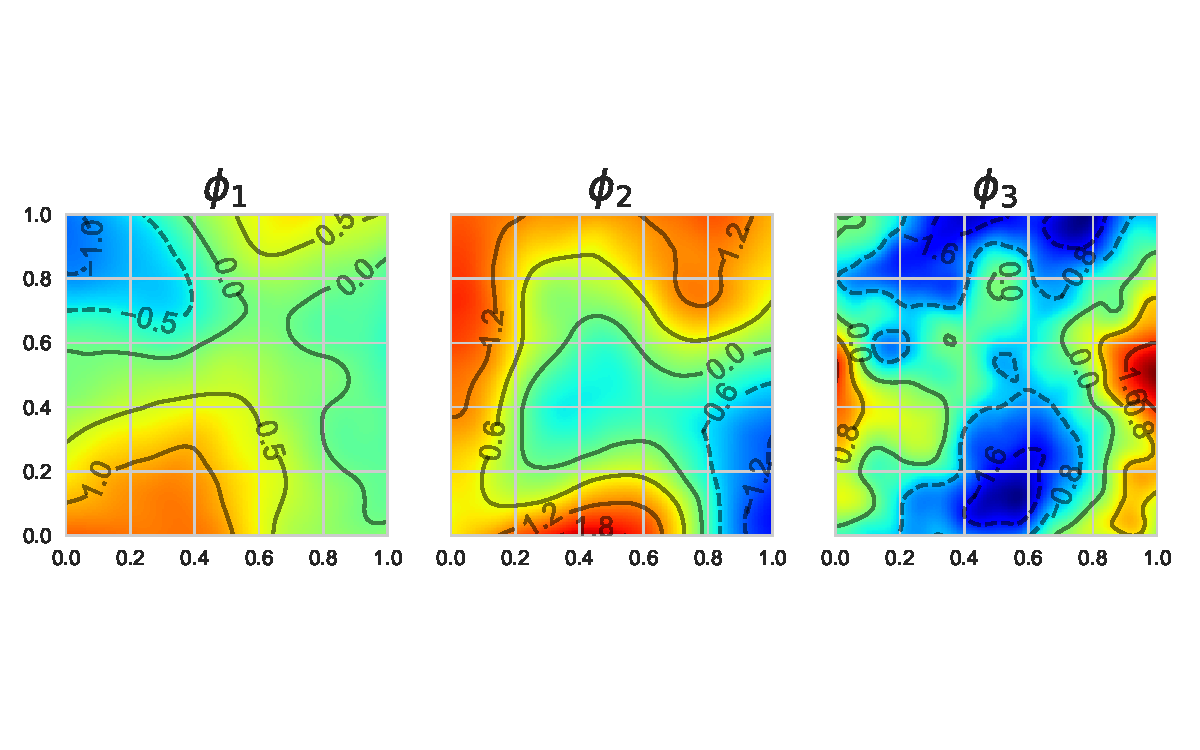
\includegraphics[width=1.0\textwidth]{sim_fpc_example}
	\caption[An example of the simulated functional principle components.]{Example of the 3 simulated principal component surfaces from the isotropic stationary Mat\`{e}rn covariance function. Notice the reduced spatial correlation in succeeding components. The simulation study is designed this way to provide difficulty for recovering the true functional principal components. }
	\label{fig:ftsm_example_fpc}
\end{figure}

To simulate the three corresponding score processes we let the variance and length scale parameters vary with each component of our decomposition.
These hyperparameters are given in Table~\ref{tab:zeta_params}.
Again we choose these parameters to emphasise the smoothness  and contribution of the leading components to the whole processes.
That is, the succeeding score processes are more variable, becoming more difficult to distinguish and forecast. 

\begin{table}[htbp!] 
	\caption[Parameters for simulating functional principal component score processes.]{The varying length scale and noise parameters in the Gaussian covariance function which is used to simulate the $3$ functional principal component scores in the data generating process.}
	\centering
	\label{tab:zeta_params}
	\begin{tabular}{l c c }
		\toprule
		& \multicolumn{2}{c}{Parameter} \\ 
		Component  & $\sigma$ &$\rho$ \\
		\midrule
		1 & 1.0 & 0.5 \\
		2 & 0.8 & 0.3 \\
		3 & 0.5 & 0.1 \\
		\bottomrule
	\end{tabular}
\end{table}

An example of the $3$ functional principal component score processes is given in Figure~\ref{fig:ftsm_example_zeta}. 
This highlights the decreasing correlation and the impact of the variance parameter on the score processes. 

\begin{figure}[htbp!] 
	\centering    
	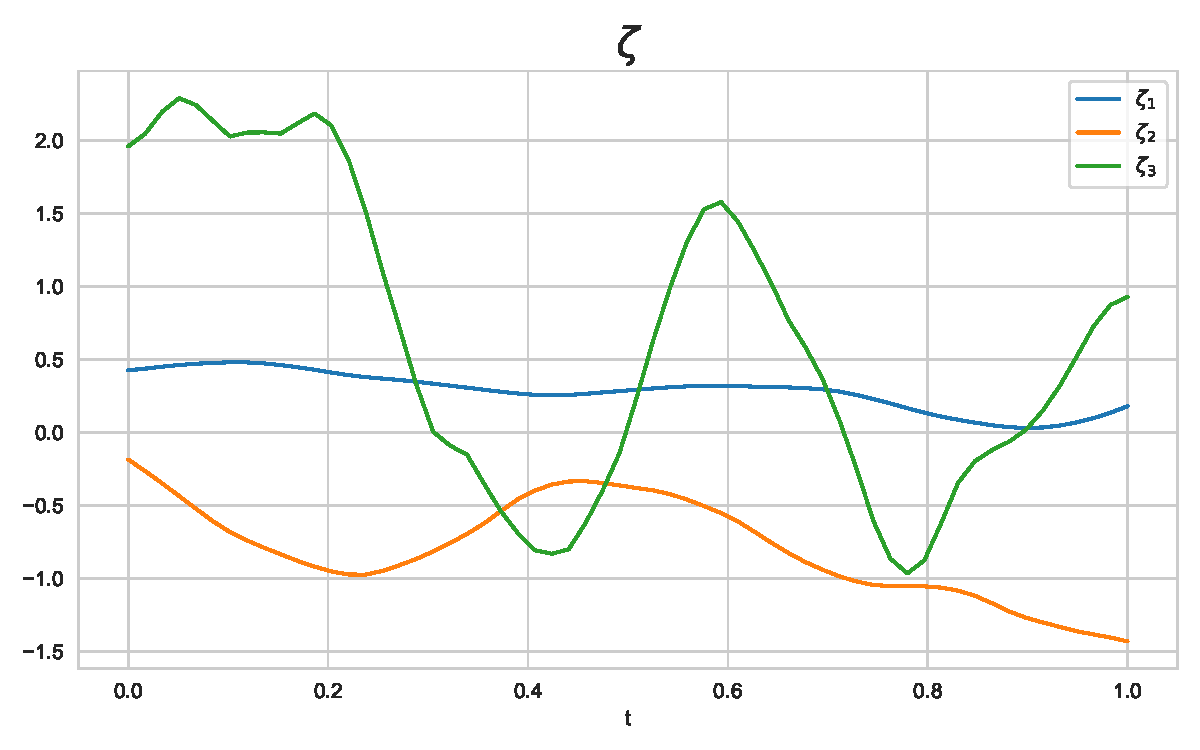
\includegraphics[width=1.0\textwidth]{sim_zeta_example}
	\caption[An example of the simulated functional principle component scores.]{Example of the 3 simulated principal component score functions from the stationary Mat\`{e}rn covariance function. Notice the reduced temporal correlation in succeeding components. The simulation study is designed this way to provide difficulty for interpolation and forecasting such components. }
	\label{fig:ftsm_example_zeta}
\end{figure}

Combining the simulated principal components with their appropriate weightings given by the simulated principal component scores, then gives us a simulation from a truncated version of the model given in Equation~\eqref{eqn:space_fpca}.
Figure~\ref{fig:ftsm_chi_example} displays a selection of time points of the corresponding functional variable simulations from the components and scores displayed in Figure~\ref{fig:ftsm_example_fpc} and Figure~\ref{fig:ftsm_example_zeta} respectively. 

\begin{figure}
	\centering
	\begin{subfigure}[b]{0.45\textwidth}
		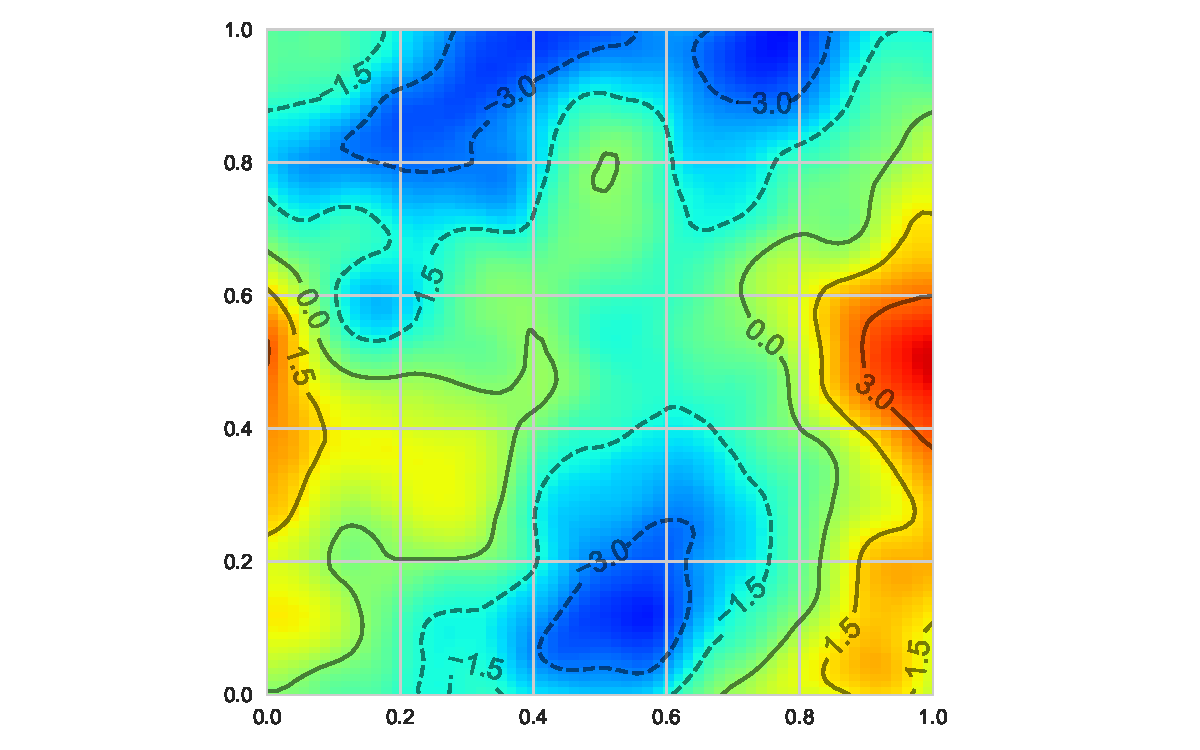
\includegraphics[width=\textwidth]{sim_chi_example_001}
		\caption{$t=0.00$}
		\label{fig:ftsm_chi_example_0}
	\end{subfigure}             
	\begin{subfigure}[b]{0.45\textwidth}
		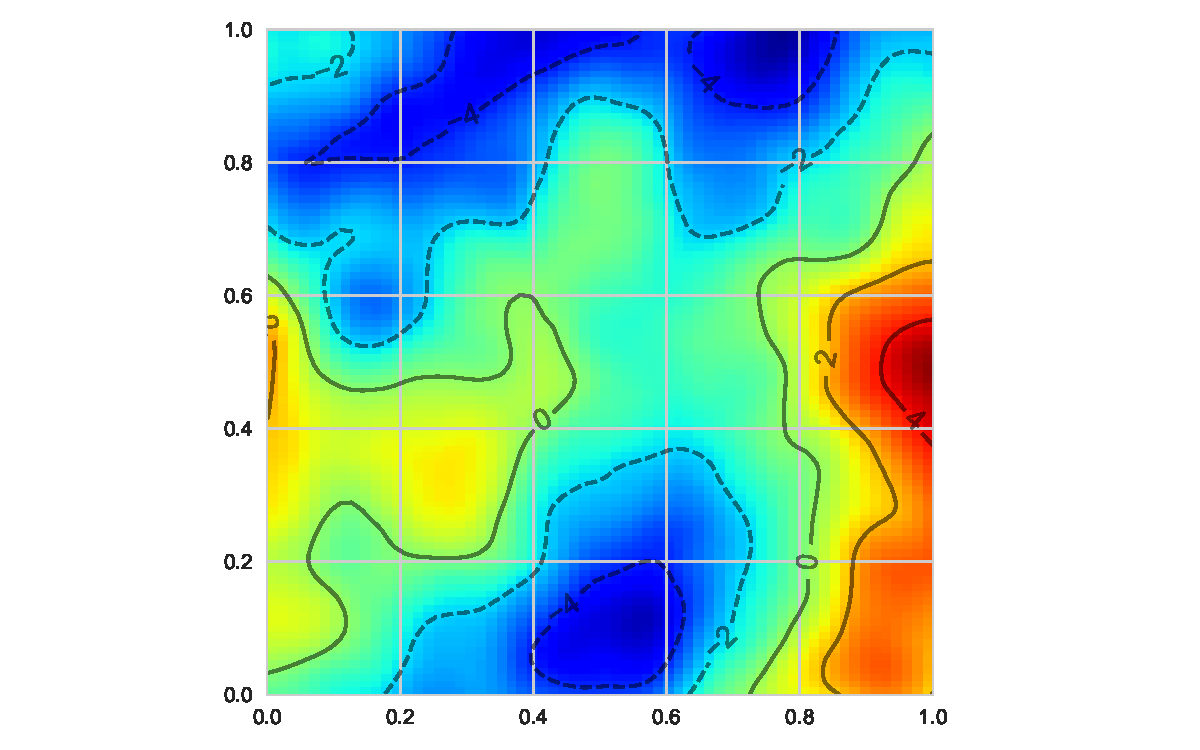
\includegraphics[width=\textwidth]{sim_chi_example_002}
		\caption{$t=0.17$}
	\end{subfigure}
	\vfill       
	\begin{subfigure}[b]{0.45\textwidth}
		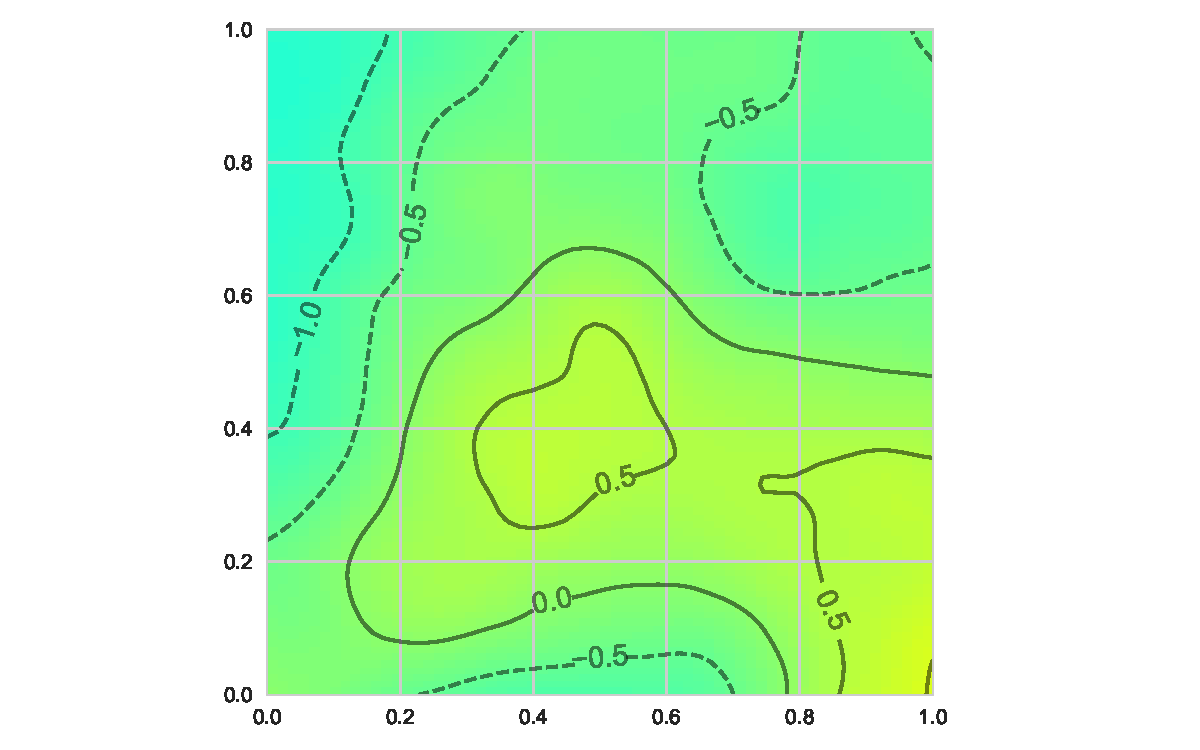
\includegraphics[width=\textwidth]{sim_chi_example_003}
		\caption{$t=0.34$}
	\end{subfigure}
	\begin{subfigure}[b]{0.45\textwidth}
		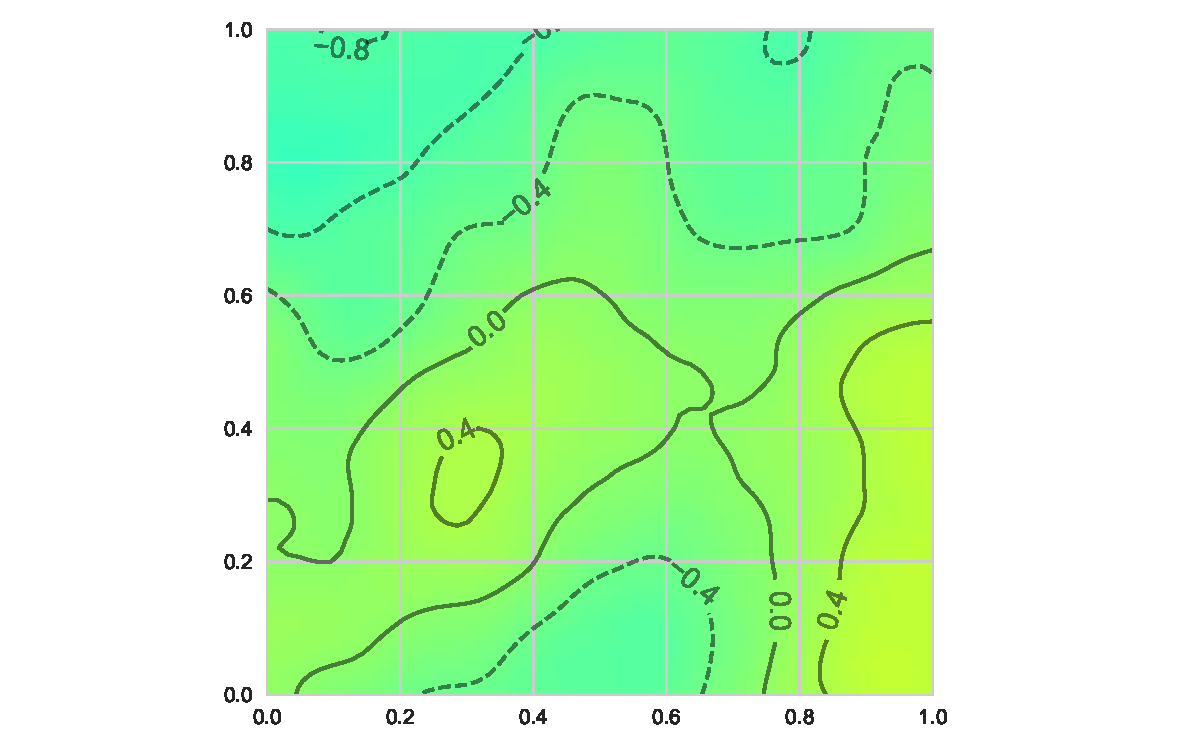
\includegraphics[width=\textwidth]{sim_chi_example_004}
		\caption{$t=0.51$}
	\end{subfigure}  
	\vfill           
	\begin{subfigure}[b]{0.45\textwidth}
		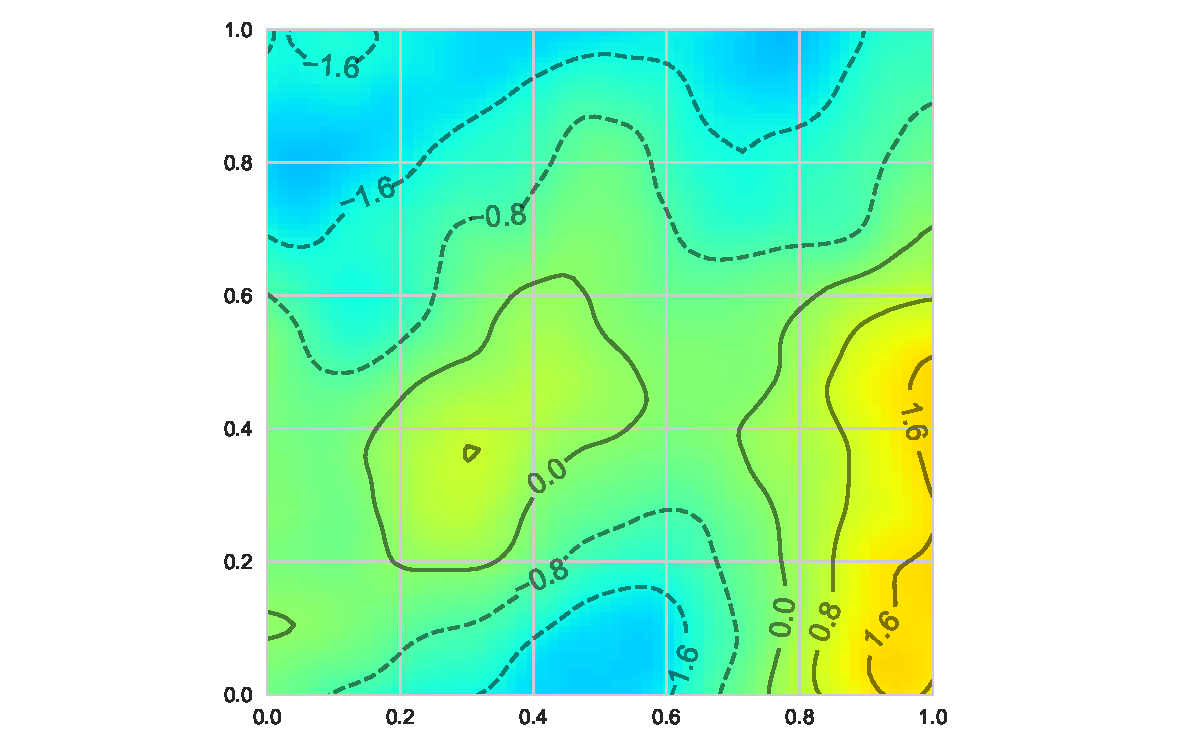
\includegraphics[width=\textwidth]{sim_chi_example_005}
		\caption{$t=0.68$}
	\end{subfigure}             
	\begin{subfigure}[b]{0.45\textwidth}
		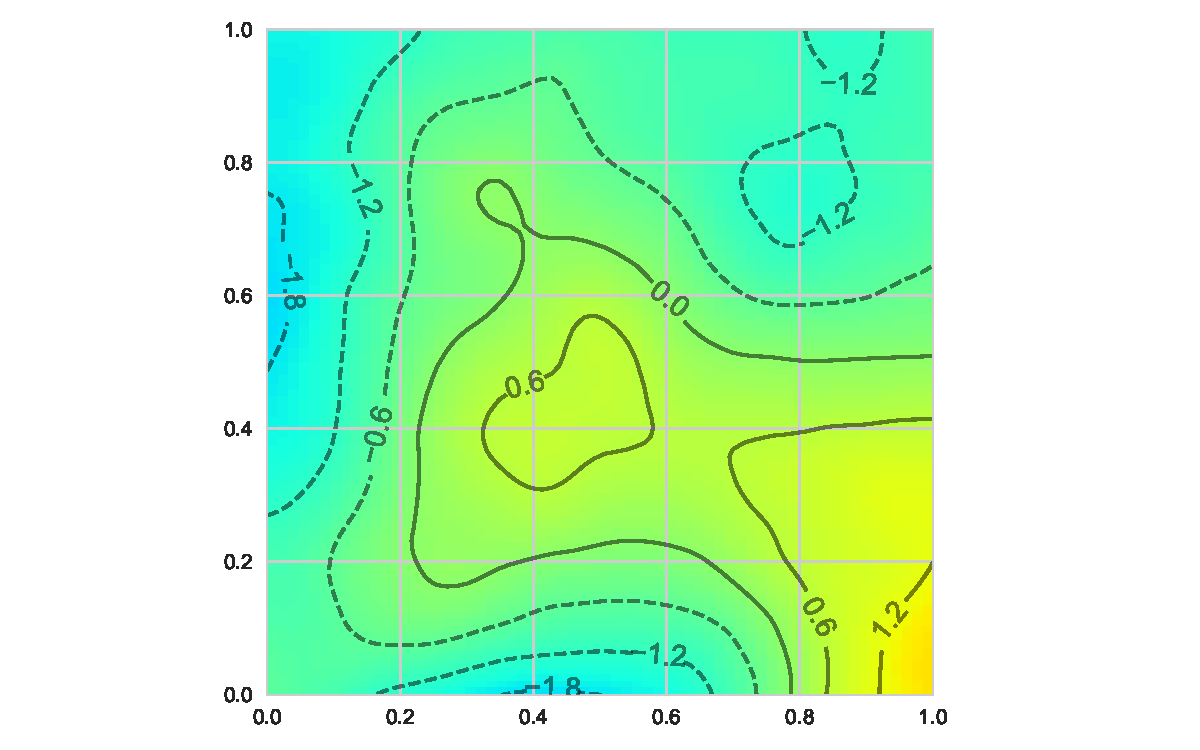
\includegraphics[width=\textwidth]{sim_chi_example_006}
		\caption{$t=0.85$}
	\end{subfigure}
	\caption[An example of simulated functional variables at various times.]{An example simulated functional variables, $\bar{\chi}_j$. for various time points, $t_j$. These correspond to the simulated functional components and scores in Figure~\ref{fig:ftsm_example_fpc} and Figure~\ref{fig:ftsm_example_zeta} respectively. Notice how we see the third principal component prominently at the beginning then fade and reappear in line with its associated score, whereas the first two components are more consistent over time.}
	\label{fig:ftsm_chi_example}
\end{figure}

As given in Equation~\eqref{eqn:space_obs}, we do not observe the simulated functional variable directly but rather with an additive noise process $\bar{\varepsilon_{ij}}$ for $i=1,2,\cdots, N$, $j=1,2,\cdots, J$.
For our simulation experiments we will consider 4 different types of observational noise; low variance independent noise (LN), high variance independent noise (HN), low variance isotropic spatially correlated noise with short range (LSN), and low variance isotropic spatially correlated noise with long range (HSN).
In all cases we assume the noise process is independent over time. 
We consider the first two (LN and HS) as corresponding to experiments to discuss how the model deals with typical measurement error. 
The second two noise models (LSN and HSN) correspond to an additional challenge to our models by testing their ability to recover the imagery, even when there is spatially correlated noise which may look similar to that of a single functional variable. 
This is of special importance in some EO data, such as satellite imagery, where often noise corresponds to atmospheric interference which is spatially correlated, \citep{oliver_understanding_2004}. 
We consider two cases where the range of the spatial correlation changes, between short range in the LSN noise and long range
 dependency in the HSN noise. 
In these two noise processes they correspond to the noise processes being spatially similar to the last and first functional principal component respectively.
 In both cases we simulate the noise process using a Gaussian process with zero mean and  Mat\`{e}rn covariance function. 
 We modulate the smoothness of the spatially dependent noise processes by modifying  the length scale parameter of the generating covariance function.
 Table~\ref{tab:ftsm_sim_noise_params} displays the noise process variance and shape parameters where applicable. 
 
\begin{table}[htbp!] 
	\caption[Parameters for simulating the noise process.]{Variance, length scale and structure parameters for the four different simulated noise processes. Independent noise over space corresponds to a blank $\nu$ and $\rho$ parameters. }
	\centering
	\label{tab:ftsm_sim_noise_params}
	\begin{tabular}{l c c  c}
		\toprule
		& \multicolumn{3}{c}{Parameter} \\ 
		Noise Type & $\sigma$ & $\rho$& $\nu$ \\
		\midrule
		LN & 0.2 & - & - \\
		HN & 1.0 & - & -\\
		LSN & 0.2 & 0.2 & 2.5 \\
		HSN & 0.2 & 0.5 & 2.5 \\
		\bottomrule
	\end{tabular}
\end{table}

The impact of such noise can be see in Figure~\ref{fig:ftsm_noise_example} which displays the imagery observed after adding the various noise types to the unobserved functional variable displayed in Figure~\ref{fig:ftsm_chi_example_0}. 

\begin{figure}
	\centering
	\begin{subfigure}[b]{0.45\textwidth}
		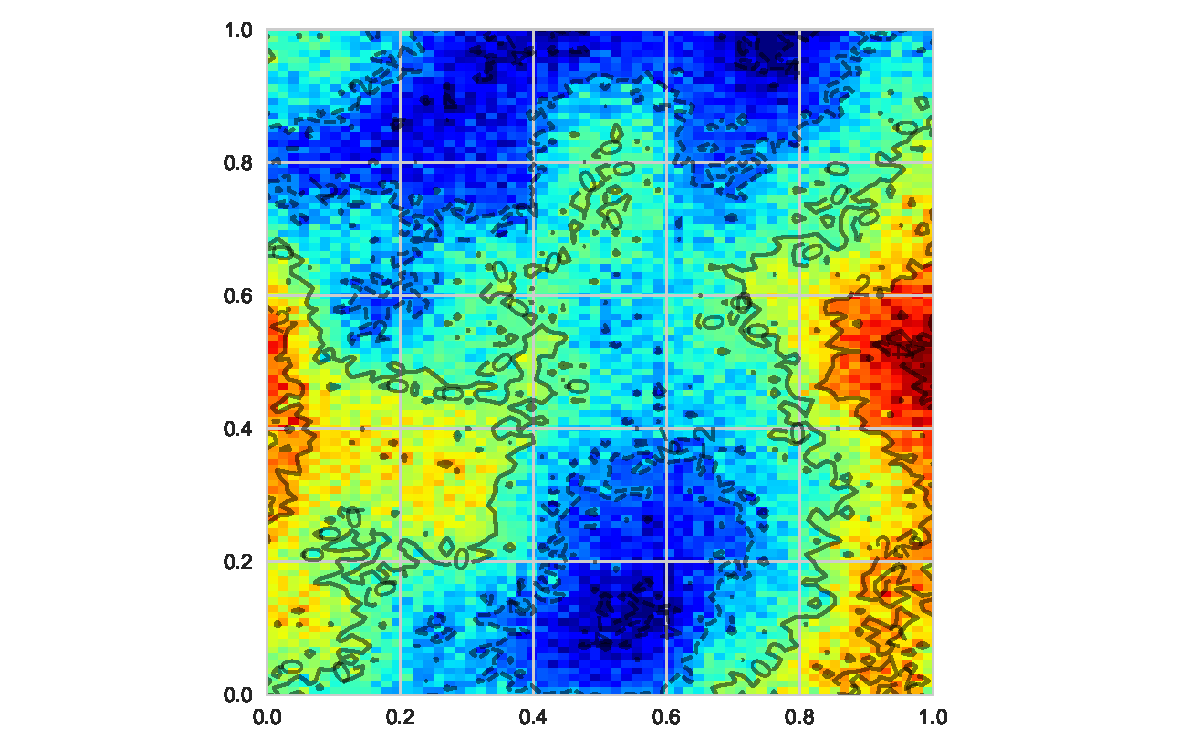
\includegraphics[width=\textwidth]{sim_noise_example_lin}
		\caption{$LN$}
		\label{fig:ftsm_noise_example_0}
	\end{subfigure}             
	\begin{subfigure}[b]{0.45\textwidth}
		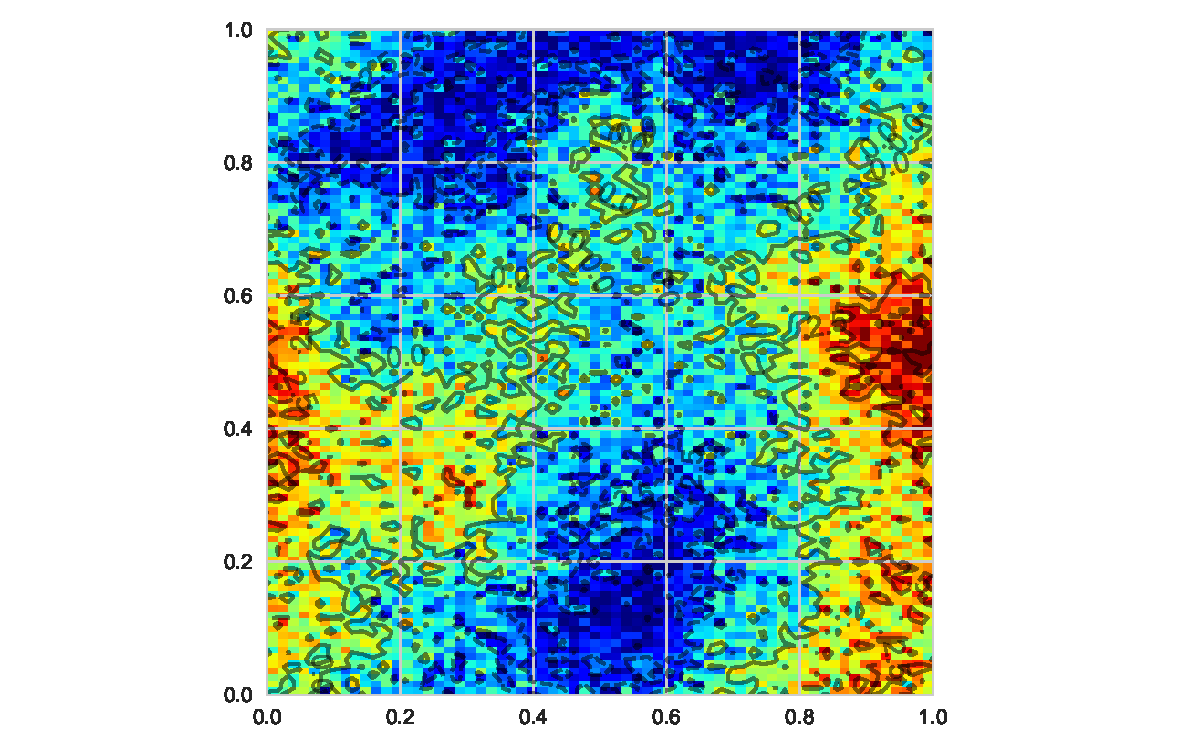
\includegraphics[width=\textwidth]{sim_noise_example_hin}
		\caption{$HN$}
	\end{subfigure}
	\vfill       
	\begin{subfigure}[b]{0.45\textwidth}
		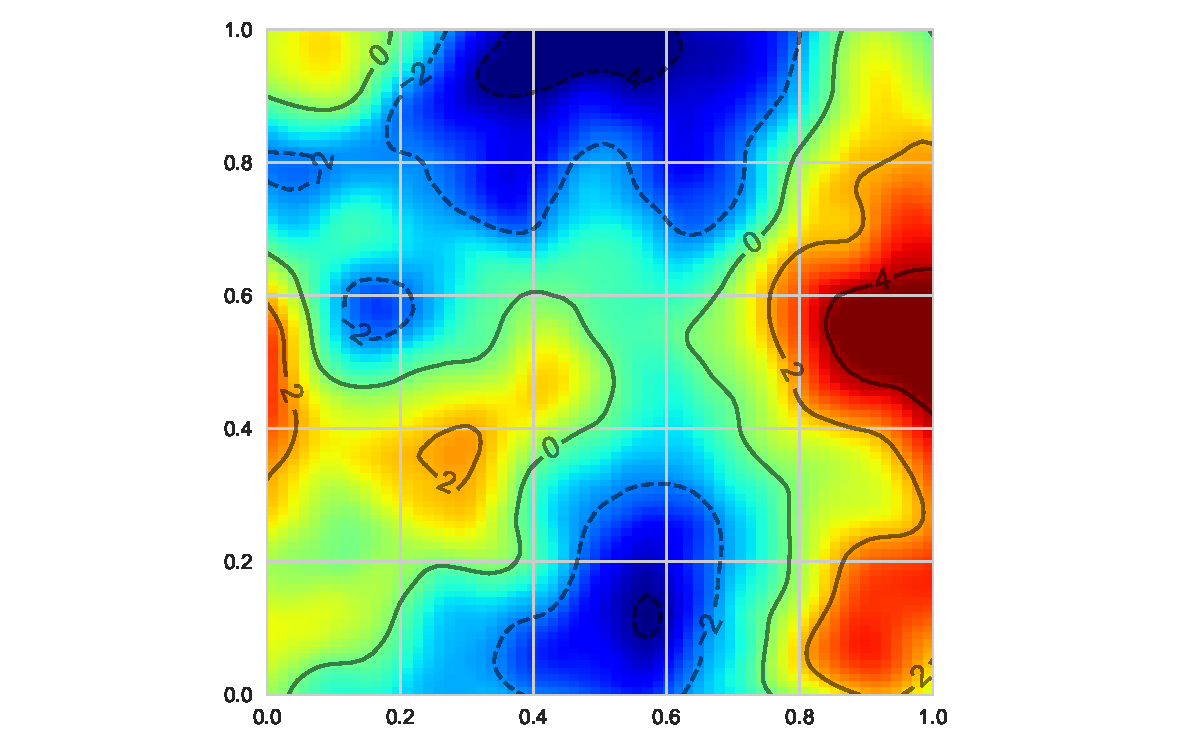
\includegraphics[width=\textwidth]{sim_noise_example_lsn}
		\caption{$LSN$}
	\end{subfigure}
	\begin{subfigure}[b]{0.45\textwidth}
		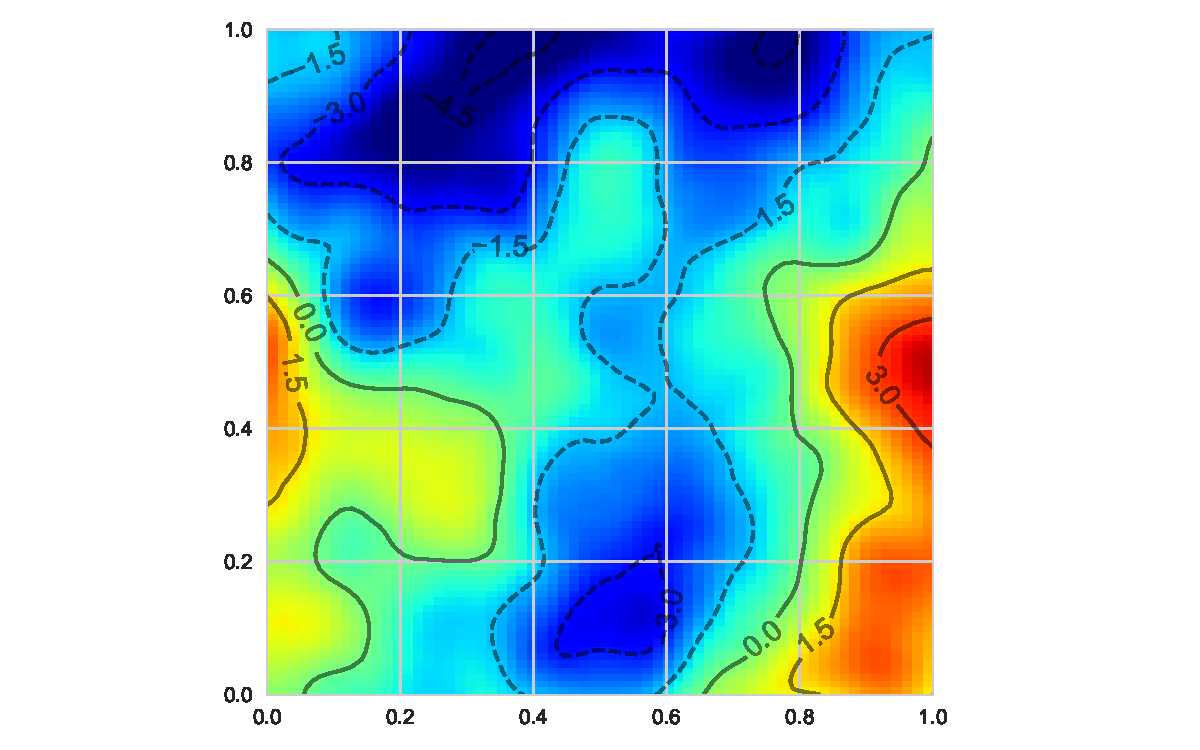
\includegraphics[width=\textwidth]{sim_noise_example_hsn}
		\caption{$HSN$}
	\end{subfigure}  
	\caption[An example of the impact of noise to observed simulated data.]{An example of the impact of the various noise structures to the observed simulated data. Each figure highlights adding a noise process to the unobserved functional variable displayed in Figure~\ref{fig:ftsm_chi_example_0}.}
	\label{fig:ftsm_noise_example}
\end{figure}

\subsection{Model parameters \label{ssec:sim_params}}
The model described in Section~\ref{sec:ftsm_model} has various hyper-parameters which control exactly how the model acts.
We specify these  below, along with justification for such choices where needed.

The first set of hyper-parameters correspond to those of the basis system used for the basis expansion of the functional variables.
In our case we limit ourselves to B-spline basis systems of order $4$, as described in Section~\ref{ssec:basis_splines}.
We choose order $4$ B-spline functions as cubic functions are the standard in many applications, \citep{de_boor_practical_2001}. 
We choose $16$ basis functions across each dimension of our surfaces, giving a total number of $256$ basis functions for the tensor product basis system, as described in Section~\ref{ssec:spline_reg}. 
This is chosen as a trade off between flexibility to fit the surface and computational constraints. 
Obviously the higher number of basis functions, the closer we can recreate the observed data.
However the additional computational cost in estimating these coefficients quickly grows as the number of basis functions in each dimension is increased.
To penalise the fitting, as described in Section~\ref{ssec:spline_reg}, we use the GCV fitting procedure given in \citep{wahba_spline_1990} with the tensor product penalty given by \citep{wood_p-splines_2017}.
We choose the penalty order to be $1$ which essentially places first derivative smoothness over the marginal basis, again such a choice is standard in spline fitting. 

The next set of hyper-parameters relates to the functional decomposition.
We choose to examine a maximum of $4$ principal components in our decomposition.
That is we set $K = 4$. 
This is chosen as to be a fairly substantive dimensionality reduction whilst maintaining a degree of representativeness, as we know through our simulation that the first $3$ components should capture the majority of the variation.
Next we set our MAFR operator $L$ to be the first order derivative.
This will again set out preference for smooth surfaces. 
Again, the first order derivative is chosen as it is often a standard in functional data analysis, \citep{ramsay_functional_2010}. 

We have already stated we choose the hyper-parameters to these processes by maximum likelihood estimation of the Gaussian process.
This estimation process is discussed in detail in \citep{williams_gaussian_2006}.

The final set of simulation hyper-parameters refers to how we split between training and testing data.
The training and test data split depends on our objective of either interpolation or forecasting.
For interpolation, we randomly select $30$ points of our time domain $\mathcal{T}$ as training points and observe the noisy simulated data at these points.
The remaining time points then represent the test data which we will evaluate our model performance against.
For forecasting, we split the time domain at the $54^\text{th}$ time point.
Any observation before this point becomes our training data with any point after being the test data which we will forecast for. 
This gives a possibility of testing long range forecasting whilst maintaining enough training data to possibly infer patterns using the score process models.

\subsection{Results \label{ssec:ftsm_sim_res}}
We present the results for interpolation and forecasting the simulated data in this section separately, as they correspond to two separate objectives.
We repeat the simulation $100$ times for both interpolation and forecasting.
The simulation results are presented separately for each of our proposed models named FPCA and MAFR.
The details of such models are described in Section~\ref{sec:ftsm_model} and the references within.

As a comparison to these methods we use a traditional PACE model using time as our functional variable.
The details of the PACE approach are set out in Section~\ref{sec:pace}.

This is a typical model for such data.
For example, \cite{hooker_maximal_2016} uses such an approach on a similar styled dataset. 
However, this approach completely ignores any spatial dependency by instead treating each pixel as independent.
Interpolation and forecasting using this methodology is performed by interpolating and extrapolating the spline basis functions in the model in standard ways, \citep{de_boor_practical_2001}.
Therefore it is mainly tailored towards interpolation, as spline regression is well known to interpolate well but extrapolate poorly, \citep{de_boor_practical_2001}.
We will denote this model by the term PACE for the following results. 


To compare these models we use four metrics. 
We use two standard measures of mean square error (RMSE) and mean absolute error (MAE).
These two are chosen to contrast the influence of any particularly large discrepancies between reconstruction and actual functional variables. 
The next metric we use is the structure similarity index (SSIM), \citep{wang_image_2004}.

The SSIM metric introduced by \citeauthor{wang_image_2004} in \citeyear{wang_image_2004} and enhanced in \citeyear{wang_mean_2009} considers the case that standard metrics such as RMSE and MAE are not indicative of perceived similarity.
For example taking a grey-scale image and adding a constant value to the whole image will increase its RMSE and MAE, however to the observer the image will only look brighter. 
SSIM tries to incorporate structural similarity when comparing imagery to highlight perceived similarity, \citep{wang_mean_2009}. 
The SSIM metric is calculated over various windows of an image.
The SSIM between two windows, x and y, of common size is given by:

\begin{equation}
	\text{SSIM}\left(x, y\right) = \frac{(2 \mu_x \mu_y + c_1)(2\sigma_{xy} + c_2)}{(\mu_x^2 + \mu_y^2 + c_1)(\sigma_x^2 + \sigma_y^2 + c_2)}
\end{equation}
where $\mu_x, \mu_y$ are the respective means of the windows, $\sigma_x, \sigma_y$ are the respective standard deviation of the windows, $\sigma_{xy}$ is the covariance of $x$ and $y$, and $c_1, c_2$ are two constants which are calculated based on the dynamic range of the two images under comparison.
For further details we refer the reader to \citep{wang_mean_2009}.
For the SSIM metric a value of one represents perfect similarity, the value of minus one represents perfect negative similarity, hence the closer to one the better for this metric.

The final metric we employ is the Peak Signal to Noise Ratio (PSNR). 
PSNR is commonly used to quantify image reconstruction quality. 
It has been used extensively in medical imaging applications.
The metric is commonly defined using the MSE between two images, $x$ and $y$ say, then the value of the metric is given by:
\begin{equation}
	\text{PSNR}(x, y) = 10 \log_{10}\left(\frac{\text{MAX}^2_x}{MSE(x,y)}\right)
\end{equation}
where $\text{MAX}_x$ is the maximum possible value in image $x$, and $MSE(x,y)$ is the mean square error between $x$ and $y$.  
For the PSNR metric a higher value is better. 

\subsubsection{Interpolation Results}
Here we present the metric results for interpolation across our test dataset as described in Section~\ref{ssec:sim_params}.
The results given are the metric values across all unobserved functional variables in the test set which we have interpolated.
We present both the average across simulations as well as the standard deviation of the metric values across simulations.

Tables~\ref{tab:ftsm_sim_interp} displays the reconstruction results for interpolation from the various observations with the different noise processes structures. 
Discussion of these results can be found in Section~\ref{ssec:ftsm_sim_disc}. 

\begin{table}[htbp!] 
	\caption[Simulation results for interpolation by noise scenario with the three models under consideration.]{Simulation results for interpolation by noise scenario for each model; PACE, FPCA, and MAFR. Bracketed values correspond to the standard deviation. Bold values illustrate best in class.}
	\centering
	\label{tab:ftsm_sim_interp}
	\begin{tabular}{l l c c c c}
		\toprule
		& & \multicolumn{4}{c}{Metric} \\ 
		Noise & Model & RMSE & MAE & SSIM & PSNR \\
		\midrule
		\multirow{3}{*}{LN}& PACE & 0.25 (0.05) & 0.20 (0.04) & 0.80 (0.07) & 28.15 (3.37) \\
		& FPCA  & \textbf{0.10 (0.05)} & \textbf{0.08 (0.04)} & \textbf{0.98 (0.02)} & \textbf{35.27 (4.59)} \\
		& MAFR  & 0.12 (0.10) & 0.10 (0.08) & 0.97 (0.02)  & 34.66 (5.08) \\
		\midrule
		\multirow{3}{*}{HN} & PACE & 0.40 (0.06) & 0.32 (0.05) & 0.58 (0.09) & 24.26 (2.93) \\
		& FPCA  & \textbf{0.16 (0.05)} & \textbf{0.13 (0.04)} & \textbf{0.95 (0.03)} & \textbf{31.78 (4.23)} \\
		& MAFR  & 0.19 (0.07) & 0.15 (0.06) & 0.94 (0.03)  & 31.06 (4.30) \\
		\midrule
		\multirow{3}{*}{LSN} & PACE & 0.50 (0.08) & 0.41 (0.07) & 0.88 (0.04) & 23.49 (2.59) \\
		& FPCA  & \textbf{0.46 (0.07)} & \textbf{0.38 (0.06)} & \textbf{0.88 (0.05)} & \textbf{23.56 (2.77)} \\
		& MAFR  & 0.48 (0.08) & 0.39 (0.06) & \textbf{0.88 (0.05)}  & 23.45 (2.56)\\
		\midrule
		\multirow{3}{*}{HSN} & PACE & 0.50 (0.10) & 0.42 (0.09) & \textbf{0.93 (0.04)} & \textbf{23.65 (3.12)}  \\
		& FPCA  & 0.51 (0.10) & 0.42 (0.09) & 0.90 (0.05) & 22.61 (2.72) \\
		& MAFR  & \textbf{0.48 (0.10)} & \textbf{0.40 (0.09)} & 0.92 (0.04) & 23.61 (2.71) \\
		\bottomrule
	\end{tabular}
\end{table}

\subsubsection{Forecasting Results}
Here we present the metric results for the forecasting ability of our models for our test dataset, as described in Section~\ref{ssec:sim_params}.
The results given are the metric value at $h$-step ahead forecasts for the unobserved functional variables in the test set where $h$ is one of $1, 3, 6$.
A single step ahead corresponds to observing the next image on our temporal grid $\mathcal{T}$ constructed in our data generating process. 
These correspond loosely to short, medium, and long range forecasts. 
This provides an overview of the abilities of the model to forecast over various ranges.
These $h$ step ahead comparisons are standard in time series forecasting, \citep{hyndman_forecasting_2021}. 
We present both the average across simulations as well as the standard deviation of the metric values across simulations.

Table~\ref{tab:ftsm_sim_for} displays the reconstruction results for each model in our simulation studies under our forecasting scenario. 
Discussion of these results can be found in Section~\ref{ssec:ftsm_sim_disc}. 

\begin{landscape}
\begin{table}
	\caption[Simulation results for forecasting by noise scenario with the three models under consideration.]{Simulation results for the models ability to forecast unseen functional variables under the FTSM model at $1, 3, 6$ time steps ahead. Bracketed values correspond to the standard deviation. Bold values illustrate best in class.}
	\centering
		
	\label{tab:ftsm_sim_for}
	\resizebox{1.6\textwidth}{!}{\begin{tabular}{l l c c c c c c c c c c c c}
		\toprule
		& & \multicolumn{12}{c}{Metric} \\ 
		 & & \multicolumn{3}{c}{RMSE} &  \multicolumn{3}{c}{MAE} &  \multicolumn{3}{c}{SSIM} &  \multicolumn{3}{c}{PSNR} \\
		Noise & Model & $h=1$ & $h=3$ & $h=6$ & $h=1$ & $h=3$ & $h=6$ & $h=1$ & $h=3$ & $h=6$ & $h=1$ & $h=3$ & $h=6$\\
		\midrule
		\multirow{3}{*}{LN} & PACE & 0.35 (0.12) & 0.68 (0.27) & 1.14 (0.49)) & 0.28 (0.09) & 0.54 (0.22) & 0.92 (0.40) & 0.60 (0.14) & 0.41 (0.17) & 0.29 (0.19) & 20.21 (3.60) & 19.18 (2.98) & 17.28 (4.03)  \\
		& FPCA  & 0.10 (0.05) & 0.28 (0.17) & \textbf{0.59 (0.33)} & \textbf{0.08 (0.04)} & 0.23 (0.14) & \textbf{0.48 (0.27)} & \textbf{0.94 (0.06)} & \textbf{0.90 (0.14)} & \textbf{0.74 (0.27)} & \textbf{28.42 (7.01)} & \textbf{25.72 (5.97)} & \textbf{20.38 (6.07)} \\
		& MAFR  & \textbf{0.10 (0.05)} & \textbf{0.28 (0.16)} & 0.60 (0.36) & \textbf{0.08 (0.04)} & \textbf{0.23 (0.13)} & 0.49 (0.29) & \textbf{0.94 (0.06)} & 0.88 (0.15) & 0.73 (0.27) & 28.04 (6.46) & 25.39 (5.60) & 20.21 (5.74) \\
		\midrule
		\multirow{3}{*}{HN} & PACE& 0.53 (0.18) & 0.90 (0.35) & 1.36 (0.54) & 0.43 (0.14) & 0.72 (0.28) & 1.09 (0.43) & 0.44 (0.11) & 0.29 (0.12) & 0.19 (0.13)  & 18.37 (2.76) & 17.62 (2.36) & 16.17 (3.28) \\
		& FPCA  & \textbf{0.17 (0.08)} & \textbf{0.34 (0.19)} & \textbf{0.63 (0.32)} & \textbf{0.14 (0.06)} & \textbf{0.28 (0.16)} & \textbf{0.52 (0.27)} & \textbf{0.90 (0.11)} & \textbf{0.86 (0.15)} & \textbf{0.72 (0.27)} & \textbf{25.62 (5.60)} & \textbf{23.81 (5.34)} & \textbf{19.47 (5.58)}  \\
		& MAFR  & \textbf{0.17 (0.08)} & 0.36 (0.19) & 0.69 (0.37) & 0.14 (0.07) & 0.29 (0.15) & 0.57 (0.31) & 0.88 (0.12) & 0.83 (0.17) & 0.70 (0.25) & 24.72 (5.61) & 22.64 (4.88) & 18.68 (5.42)  \\
		\midrule
		\multirow{3}{*}{LSN} & PACE & 0.74 (0.26) & 1.21 (0.49) & 1.72 (0.64) & 0.61 (0.22) & 1.00 (0.42) & 1.42 (0.54) & 0.76 (0.13) & 0.63 (0.19) & 0.47 (0.26)  & 18.37 (3.28) & 16.54 (3.21) & 14.12 (3.57) \\
		& FPCA  & \textbf{0.54 (0.24)} & \textbf{0.70 (0.35)} & \textbf{0.90 (0.45)} & \textbf{0.44 (0.19)} & \textbf{0.58 (0.28)} & \textbf{0.74 (0.38)} & 0.77 (0.20) & 0.70 (0.25) & 0.59 (0.31) & \textbf{19.86 (4.72)} & \textbf{18.52 (4.56)} & \textbf{16.53 (4.96)}  \\
		& MAFR  & 0.56 (0.20) & 0.74 (0.30) & 0.97 (0.44) & 0.47 (0.16) & 0.61 (0.25) & 0.80 (0.37) & \textbf{0.78 (0.17)} & \textbf{0.72 (0.21)} & \textbf{0.61 (0.28)} & 19.54 (4.32) & 18.29 (4.21) & 16.22 (4.42) \\
		\midrule
		\multirow{3}{*}{HSN} & PACE & 0.74 (0.29) & 1.21 (0.47) & 1.71 (0.68) & 0.62 (0.25) & 1.01 (0.42) & 1.43 (0.60) & \textbf{0.82 (0.13)} & 0.70 (0.21) & 0.54 (0.32) & 18.45 (3.34) & 17.01 (3.37) & 14.86 (4.17)  \\
		& FPCA  & 0.60 (0.23) & 0.75 (0.34) & \textbf{0.94 (0.46)} & 0.50 (0.19) & \textbf{0.62 (0.29)} & \textbf{0.78 (0.39)} & 0.79 (0.20) & \textbf{0.74 (0.22)} & 0.62 (0.29) & 19.87 (4.97) & 18.83 (4.89) & 16.43 (4.75)  \\
		& MAFR  & \textbf{0.59 (0.24)} & \textbf{0.75 (0.33)} & 0.97 (0.46) & \textbf{0.49 (0.21)} & 0.63 (0.28) & 0.81 (0.40) & 0.82 (0.17) & 0.76 (0.21) & \textbf{0.64 (0.30)}  & \textbf{20.22 (4.83)} & \textbf{18.98 (4.66)} & \textbf{16.65 (4.85)} \\
		\bottomrule
	\end{tabular}}
\end{table}
\end{landscape}

\subsection{Discussion \label{ssec:ftsm_sim_disc}}

We discuss the preceding results for the FPCA and MAFR models in the following section.
We discuss the results relative to the PACE model as described in Section~\ref{ssec:ftsm_sim_res} under both the interpolation and forecasting objectives.

Table~\ref{tab:ftsm_sim_interp} states the mean and standard deviations of the estimation error under the various metrics discussed in Section~\ref{ssec:ftsm_sim_res} for the interpolation metric.
We can see clearly an advantage of using the FPCA model over the PACE model under most metrics in nearly all noise process scenarios.
The only exception to this being under the highly structured spatial noise process, denoted by HSN, where the FPCA model is inferior to the MAFR and PACE models; though only slightly.
This advantage is most prominent under the independent noise scenarios, where it seems that the additional spatial smoothness constraints that the model enforces nullifies the impact of the spatially independent noise.
Similarly, the relative deterioration in the FPCA model under structured noise agrees with this effect.
In fact, it is possible that due to the noise process being highly similar to the leading functional principal components in the HSN scenario that the FPCA model may conflate the two, hence giving reduced performance.

The MAFR model has similar performance to that of the FPCA model; as expected, due to it being a rotated version of the FPCA model.
It is narrowly but consistently beaten on most noise scenarios, except for the HSN.
Here, the fact that the MAFR model prioritises smoothness in its components, \citep{hooker_maximal_2016}, has meant that we have overcome some of the trouble that the FPCA model faced in conflating the noise and signal processes. 
We can see this effect by examining the second functional principal component for both the FPCA and MAFR model for a single simulation under the HSN noise scenario as an example.
Figure~\ref{fig:ftsm_res_example_fpc} shows exactly this.
The actual functional principal components for this simulation are given in Figure~\ref{fig:ftsm_example_fpc}.

\begin{figure}[!htbp]
	\centering
	\begin{subfigure}[b]{0.45\textwidth}
		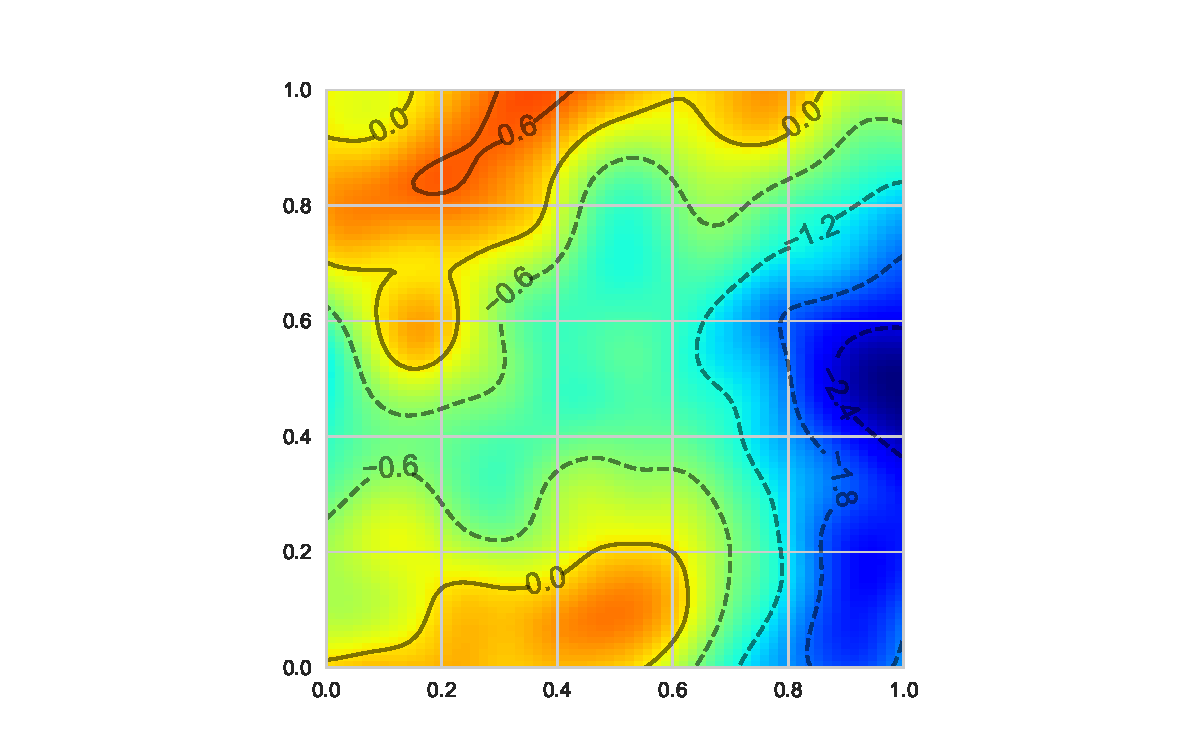
\includegraphics[width=\textwidth]{ftsm_res_fpc_example_fpca}
		\caption{FPCA}
	\end{subfigure}             
	\begin{subfigure}[b]{0.45\textwidth}
		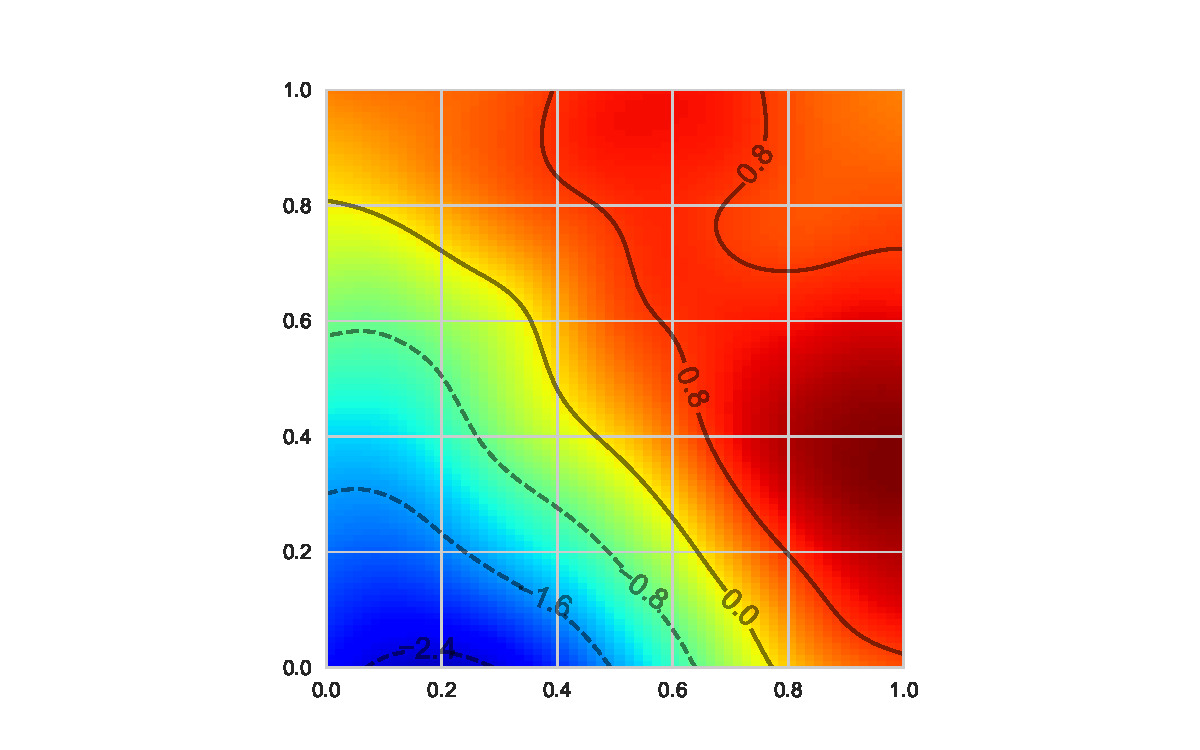
\includegraphics[width=\textwidth]{ftsm_res_fpc_example_mafr}
		\caption{MAFR}
	\end{subfigure}
	\caption[Comparison of the second functional principal component under FPCA and MAFR models.]{Comparison of the second functional principal component recovered under the FPCA model and the MAFR model for an example simulation under the HSN noise scenario. Notice how the MAFR component is much smoother over the domain.}
	\label{fig:ftsm_res_example_fpc}
\end{figure}

In addition, this rotation has caused the score processes to be correlated to the point that leading components will have smoother scores, aiding in removing the noise process which will have random walk like behaviour in the scores process, due to it being independent over time.
This is illustrated in Figure~\ref{fig:ftsm_res_example_zeta} where we can see that although both score processes aren't particularly smooth, the MAFR process exhibits less variation. 

\begin{figure}[htbp!] 
	\centering    
	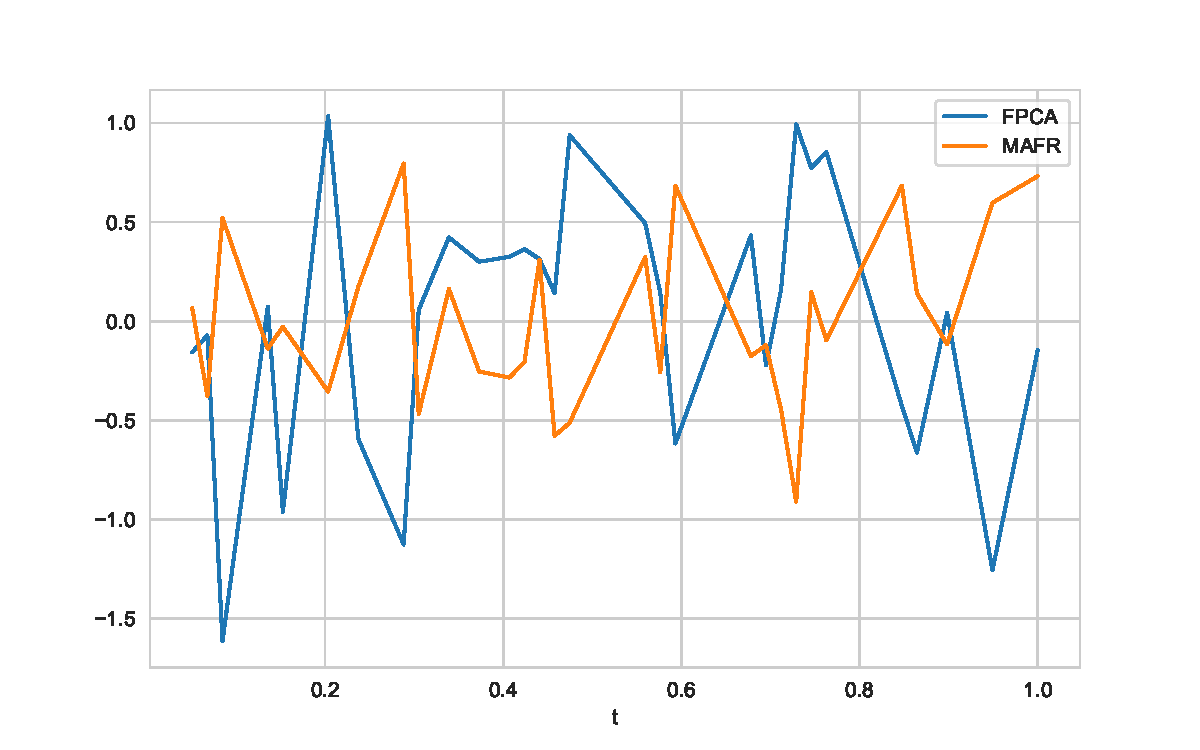
\includegraphics[width=1.0\textwidth]{ftsm_res_zeta_example}
	\caption[Comparison of the second score process under FPCA and MAFR models.]{Comparison of the second score process corresponding to the second functional principal component given in Figure~\ref{fig:ftsm_res_example_fpc}. Notice how the MAFR score process exhibits less variation over time compared to the FPCA process.}
	\label{fig:ftsm_res_example_zeta}
\end{figure}

The results for the forecasting objective are given in Table~\ref{tab:ftsm_sim_for}.
Here, we see similar results to that which were observed in the interpolation objective.
We see both the FPCA and MAFR models outperform the PACE model under most noise scenarios.
Similarly to the interpolation results we see the most improvement under spatially independent noise processes.
Again, this is due to the added ability of the FPCA and MAFR models to filter out any process which isn't particularly smooth over space. 
Interestingly, we also see a greater improvement in reconstruction for the long term forecast rather than the one step ahead short term forecast relative to the PACE model.
This is good as it suggests that the FPCA and MAFR approaches capture the spatio-temporal process in such a way that is easier to forecast. 
Figure~\ref{fig:ftsm_res_recon} highlights this ability by illustrating the unobserved surface and estimated surfaces for each model under the LN noise scenario at three time steps ahead.

\begin{figure}
	\centering
	\begin{subfigure}[b]{0.45\textwidth}
		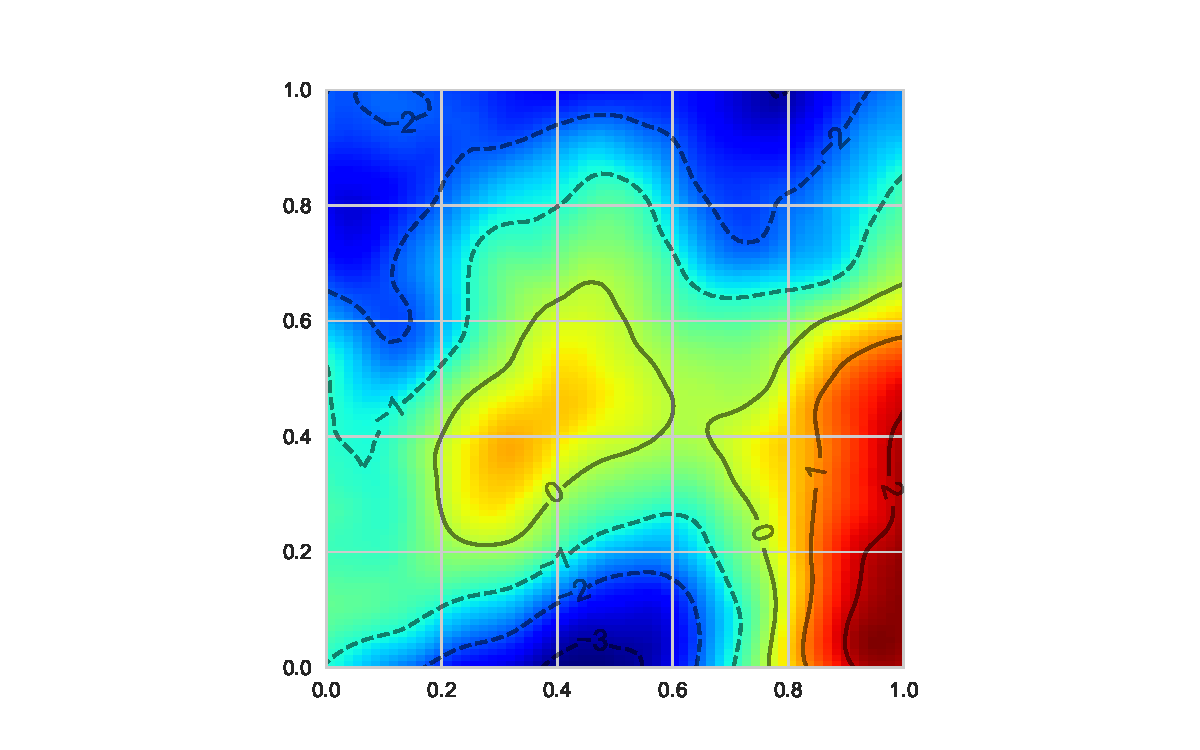
\includegraphics[width=\textwidth]{ftsm_res_recon_example_unob}
		\caption{$Unobserved$}
		\label{fig:ftsm_res_recon_unob}
	\end{subfigure}             
	\begin{subfigure}[b]{0.45\textwidth}
		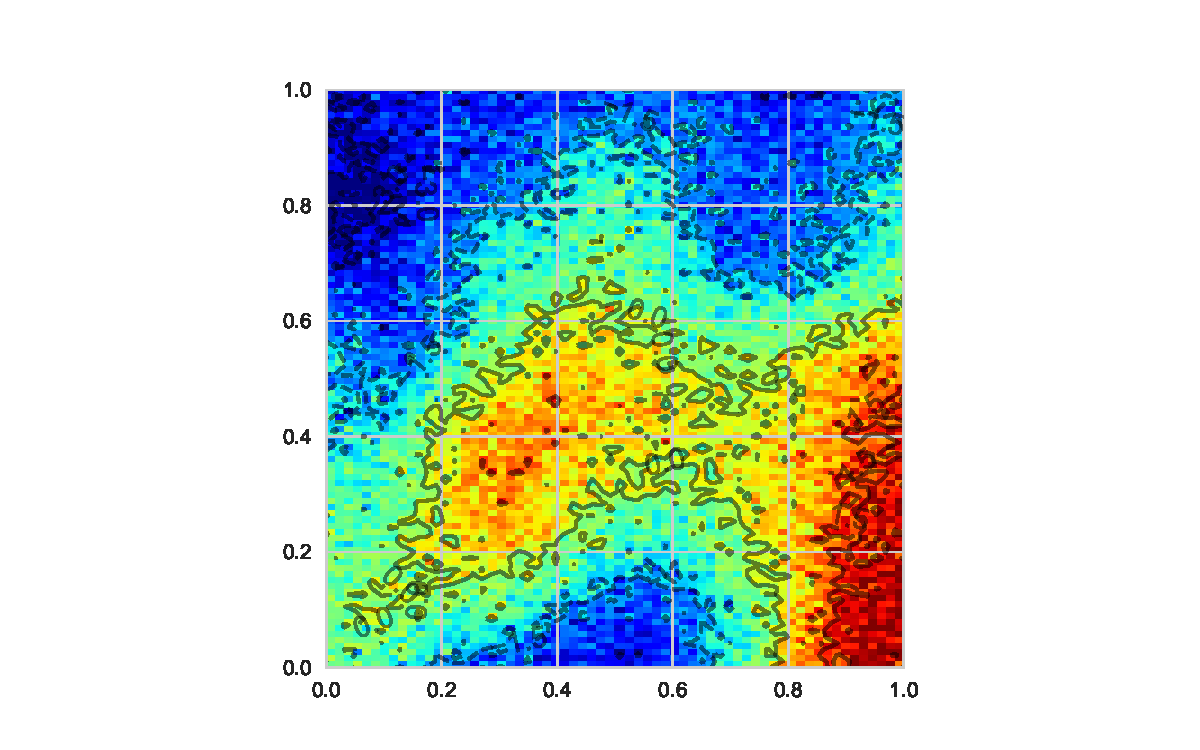
\includegraphics[width=\textwidth]{ftsm_res_recon_example_pace}
		\caption{$PACE$}
		\label{fig:ftsm_res_recon_pace}
	\end{subfigure}
	\vfill       
	\begin{subfigure}[b]{0.45\textwidth}
		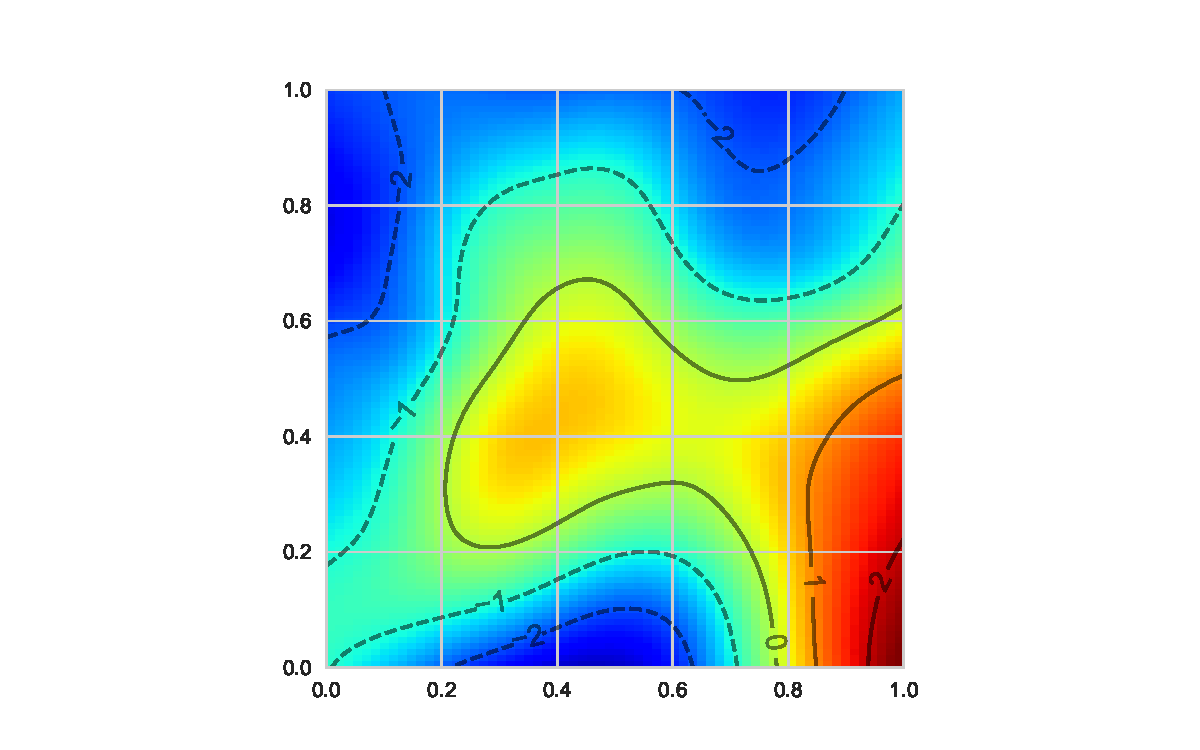
\includegraphics[width=\textwidth]{ftsm_res_recon_example_fpca}
		\caption{$FPCA$}
		\label{fig:ftsm_res_recon_fpca}
	\end{subfigure}
	\begin{subfigure}[b]{0.45\textwidth}
		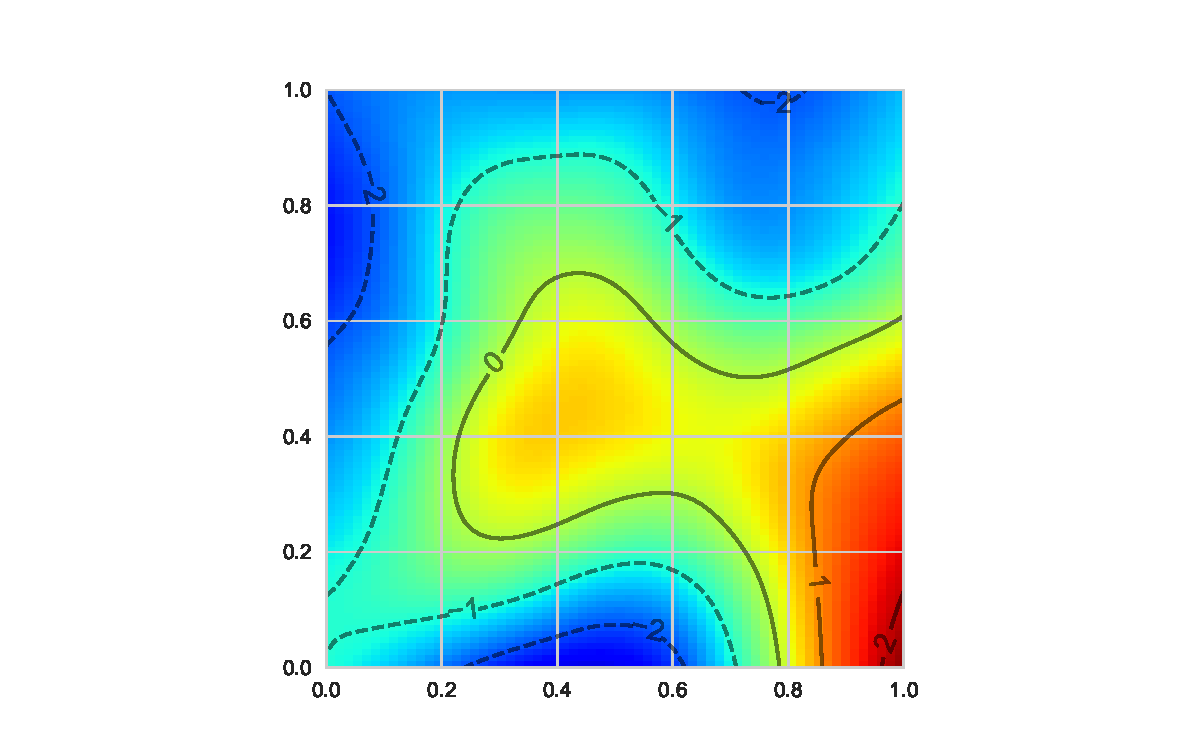
\includegraphics[width=\textwidth]{ftsm_res_recon_example_mafr}
		\caption{$MAFR$}
		\label{fig:ftsm_res_recon_mafr}
	\end{subfigure}  
	\caption[Example of the impact of the various models to reconstruct the unobserved surface at three steps ahead.]{Example of the impact of the various models to reconstruct the unobserved surface at three steps ahead. The observed process was corrupted by the LN noise process. We note how the PACE model is easily over fitting to the independent noise process whereas the FPCA and MAFR models do not suffer this effect.}
	\label{fig:ftsm_res_recon}
\end{figure}

Again the FPCA and MAFR approaches lead to similar results, with the FPCA model edging the results for the majority of the noise processes.
Similarly to the interpolation results we see that the MAFR model tends to perform better under the HSN noise scenario. 
This is due to the same reasons as the interpolation results described above. 

These results offer a good indication that including spatial information into the model for such datasets can have a material impact on both interpolating and forecasting objectives. 
The next test for such models is then to see how this improvement translates to datasets not necessarily coming from the assumed data generating procedure.
We consider this by applying these model to our EO dataset as discussed in Chapter~\ref{cha:data} in the next section. 

\section{EO Application \label{sec:ftsm_eo}}
We apply the same models as used in the simulation model to our CESM-LE dataset as described in Chapter~\ref{cha:data}.
This dataset acts as an example to highlight the performance of the various models described above on a real world dataset. 
We perform the exact same analysis as in the simulation study but this time apply it to the $40$ replications of the CESM-LE data for the various atmospheric variable. 

We use the exact same model parameter setup as described in Section~\ref{ssec:sim_params} to setup the models for the EO application study.
We detail the results of the study in Section~\ref{ssec:ftsm_eo_res}.

\subsection{Results \label{ssec:ftsm_eo_res}}
We present the reconstruction results for the objectives of interpolation and forecasting separately. 
We repeat the model fitting and reconstruction procedure independently for the $40$ realisations of the CESM-LE dataset and provide both the mean metric measures as well as their standard deviations across these realisations. 
We use the same $4$ metrics as used in the simulation study for consistency. 

\subsubsection{Interpolation Results}
Here we present the metric results for interpolation for our test dataset from our CESM-LE EO observations, as described in Chapter~\ref{cha:data}.
See Section~\ref{ssec:sim_params} for the construction methodology of the test and training datasets. 
The results given are the metric values across all unobserved functional variables in the test set which we have interpolated.
We present both the average across simulations as well as the standard deviation of metric values across simulations.

Table~\ref{tab:ftsm_eo_interp} displays the reconstruction results for interpolation from the various atmospheric variables.
Discussion of these results can be found in Section~\ref{ssec:ftsm_eo_disc}.

\begin{table}[htbp!] 
	\caption[Results for interpolation by atmospheric components with various FTSM models for the CESM-LE dataset.]{Results for interpolation by atmospheric components with various FTSM models for the CESM-LE dataset. Bracketed values correspond to the standard deviation.}
	\centering
	\label{tab:ftsm_eo_interp}
	\resizebox{\textwidth}{!}{\begin{tabular}{l l c c c c}
		\toprule
		& & \multicolumn{4}{c}{Metric} \\ 
		Component & Model & RMSE & MAE & SSIM & PSNR \\
		\midrule
		\multirow{3}{*}{TMQ}&PACE & \textbf{5.60 (0.52)} & \textbf{4.31 (0.47)} & \textbf{0.73 (0.05)} & \textbf{18.61 (1.49)} \\
		& FPCA  & 6.08 (0.30) & 4.56 (0.25) & 0.70 (0.01) & 18.19 (0.52) \\
		& MAFR  &6.03 (0.30) & 4.52 (0.25) & 0.70 (0.01)  & 18.39 (0.75) \\
		\midrule
		\multirow{3}{*}{PS} & PACE & \textbf{511.40 (30.69)} & \textbf{374.56 (22.04)} & \textbf{0.99 (0.00)} & \textbf{33.83 (3.35)} \\
		& FPCA  & 2976.61 (4.81) & 1814.34 (6.92) & 0.70 (0.00) & 21.50 (0.49) \\
		& MAFR  & 2977.02 (5.68) & 1815.04 (7.44) & 0.70 (0.00)  & 21.51 (0.52) \\
		\midrule
		\multirow{3}{*}{TREFHT} & PACE & \textbf{6.80 (1.05)} & \textbf{5.05 (0.84)} & \textbf{0.90 (0.02)} & \textbf{23.69 (2.58)} \\
		& FPCA  & 7.45 (0.35) & 5.33 (0.25) & 0.84 (0.00) & 20.43 (0.44) \\
		& MAFR  & 7.48 (0.47) & 5.38 (0.37) & 0.83 (0.00)  & 20.39 (0.36)\\
		\midrule
		\multirow{3}{*}{U10} & PACE & \textbf{1.25 (0.12)} & \textbf{0.92 (0.08)} & \textbf{0.76 (0.03)} & \textbf{19.27 (1.70)}  \\
		& FPCA  & 1.55 (0.03) & 1.20 (0.02) & 0.55 (0.00) & 16.33 (0.77) \\
		& MAFR  &1.55 (0.03) & 1.19 (0.02) & 0.55 (0.00) & 16.32 (0.81) \\
		\bottomrule
	\end{tabular}}
\end{table}

\subsubsection{Forecasting Results}
Here we present the metric results for the forecasting ability of our models for our test dataset from our CESM-LE EO observations, as described in Chapter~\ref{cha:data}.
See Section~\ref{ssec:sim_params} for the construction methodology of the test and training datasets. 
The results given are the metric value at $h$-step ahead forecasts for the unobserved functional variables in the test set where $h$ is one of $1, 3, 6$. 
These correspond to short, medium, and long range forecasts.
In the CESM-LE dataset each step corresponds to a month interval.
This provides an overview of the abilities of the model to forecast over various ranges.
We present both the average across simulations as well as the standard deviation of the metric values across simulations.

Table~\ref{tab:ftsm_eo_for} displays the reconstruction results for each model in our simulation studies under our forecasting scenario. 
Discussion of these results can be found in Section~\ref{ssec:ftsm_eo_disc}.

\begin{landscape}
	\begin{table}
		\caption[Results for forecasting by variable with various FTSM model on the CESM-LE dataset.]{Results for the models ability to forecast unseen functional variables under the FTSM models at $1, 3, 6$ time steps ahead in the CESM-LE dataset. Bracketed values correspond to the standard deviation. Bold represents best in class.}
		\centering
		\label{tab:ftsm_eo_for}
		\resizebox{1.6\textwidth}{!}{\begin{tabular}{l l c c c c c c c c c c c c}
			\toprule
			& & \multicolumn{12}{c}{Metric} \\ 
			& & \multicolumn{3}{c}{RMSE} &  \multicolumn{3}{c}{MAE} &  \multicolumn{3}{c}{SSIM} &  \multicolumn{3}{c}{PSNR} \\
			Noise & Model & $h=1$ & $h=3$ & $h=6$ & $h=1$ & $h=3$ & $h=6$ & $h=1$ & $h=3$ & $h=6$ & $h=1$ & $h=3$ & $h=6$\\
			\midrule
			\multirow{3}{*}{TMQ} & PACE & \textbf{3.50 (0.67)} & \textbf{5.92 (1.34)} & 5.81 (2.20) & \textbf{2.41 (0.54)} & \textbf{4.71 (1.04)} & 4.17 (1.72) & 0.45 (0.02) & 0.51 (0.03) & 0.39 (0.03) & 12.22 (0.50) & 13.30 (0.48) & 11.78 (0.46)  \\
			& FPCA  & 4.11 (0.46) & 9.62 (1.17) & 5.16 (0.86) & 2.71 (0.36) & 7.48 (0.99) & 3.65 (0.67) & \textbf{0.77 (0.01)} & \textbf{0.60 (0.05)} & \textbf{0.72 (0.03)} & 20.30 (0.89) & \textbf{16.27 (1.10)} & 18.96 (1.03)  \\
			& MAFR  & 4.12 (0.52) & 9.61 (1.20) & \textbf{5.12 (0.98)} & 2.75 (0.42) & 7.46 (1.02) & \textbf{3.62 (0.77)} & 0.77 (0.02) & \textbf{0.60 (0.05)} & \textbf{0.72 (0.03)} & \textbf{20.33 (0.84)} & 16.24 (1.11) & \textbf{19.00 (0.86)} \\
			\midrule
			\multirow{3}{*}{PS} & PACE & \textbf{572.92 (254.02)} & \textbf{1416.61 (3179.94)} & 4167.61 (19882.51) & \textbf{440.70 (243.79)} & \textbf{1176.94 (3209.63)} & 3919.64 (19920.73) & \textbf{0.98 (0.06)} & \textbf{0.98 (0.06)}  & \textbf{0.97 (0.07)} & \textbf{32.54 (5.30)} & \textbf{33.17 (5.42)} & \textbf{33.09 (5.88)}\\
			& FPCA  & 2963.55 (16.73) & 2962.08 (13.00) & 2967.76 (11.98) & 1801.39 (26.40) & 1800.56 (20.45) & 1810.16 (24.96) & 0.70 (0.00) & 0.70 (0.00) & 0.69 (0.00) & 20.96 (0.46) & 21.03 (0.46) & 21.16 (0.44)  \\
			& MAFR  & 2962.67 (17.11) & 2962.55 (15.21) & \textbf{2965.04 (9.17)} & 1800.63 (27.52) & 1802.48 (25.31) & \textbf{1804.88 (20.88)} & 0.70 (0.00) & 0.70 (0.00) & 0.69 (0.00) & 20.96 (0.36) & 21.03 (0.38) & 21.17 (0.35)  \\
			\midrule
			\multirow{3}{*}{TREFHT} &PACE & 10.13 (0.59) & 27.36 (1.16) & 30.60 (1.13) & 6.90 (0.36) & 18.52 (0.80) & 20.17 (0.79) & 0.81 (0.01) & \textbf{0.81 (0.01)} & 0.59 (0.01)  & 17.48 (0.54) & 18.04 (0.68) & 17.03 (0.49)  \\
			& FPCA  & \textbf{5.87 (1.31)} & \textbf{10.75 (1.66)} & \textbf{4.42 (1.05)} & \textbf{4.03 (0.89)} & \textbf{7.66 (1.28)} & \textbf{3.34 (0.83)} & \textbf{0.85 (0.02)} & 0.77 (0.03) & \textbf{0.85 (0.01)} & \textbf{21.59 (1.39)} & \textbf{18.80 (1.59)} & \textbf{21.56 (0.77)}  \\
			& MAFR  & 6.29 (1.05) & 11.30 (1.36) & 4.65 (1.18) & 4.36 (0.73) & 8.12 (1.15) & 3.56 (1.01) & 0.84 (0.01) & 0.76 (0.02) & 0.84 (0.02) & 21.19 (1.00) & 18.26 (1.15) & 21.40 (0.85) \\
			\midrule
			\multirow{3}{*}{U10} & PACE & \textbf{1.21 (0.07)} & \textbf{1.51 (0.12)} & \textbf{1.27 (0.11)} & \textbf{0.91 (0.06)} & \textbf{1.11 (0.10)} & \textbf{0.92 (0.08)} & \textbf{0.78 (0.02)} & \textbf{0.71 (0.03)} & \textbf{0.74 (0.03)} & \textbf{21.47 (0.74)} & \textbf{19.84 (0.88)} & \textbf{21.31 (0.82)}  \\
			& FPCA  & 1.43 (0.06) & 1.75 (0.11) & 1.41 (0.06) & 1.12 (0.05) & 1.34 (0.09) & 1.10 (0.05) & 0.56 (0.02) & 0.50 (0.03) & 0.56 (0.02) & 16.50 (0.83) & 16.05 (0.85) & 17.03 (0.74)  \\
			& MAFR  & 1.43 (0.05) & 1.75 (0.09) & 1.41 (0.04) & 1.12 (0.05) & 1.34 (0.08) & 1.10 (0.04) & 0.56 (0.02) & 0.49 (0.02) & 0.56 (0.02)  & 16.37 (0.61) & 15.93 (0.59) & 16.91 (0.53) \\
			\bottomrule
		\end{tabular}}
	\end{table}
\end{landscape}

\subsection{Discussion \label{ssec:ftsm_eo_disc}}
We discuss the preceding results for the FPCA and MAFR models with application on the CESM-LE dataset in the following section.
We discuss the results relative to the PACE model as described in Section~\ref{ssec:ftsm_sim_res} under both the interpolation and forecasting objectives.

Evidently, from Table~\ref{tab:ftsm_eo_interp}, the PACE model outperforms both the FPCA and MAFR models for all atmospheric variables studied across all metrics.
This is particularly the case for the PS and U10 variables. 
The reason for this divergence from the PACE model can be seen by considering an example from the PS variable.
Figure~\ref{fig:ftsm_res_ps} gives the unobserved surface and the estimated surfaces from the PACE, FPCA, and MAFR models.
We can clearly see from this that the FPCA and MAFR models, although capturing large scale spatial patterns, they fail to capture the small scale spatial variation which is present in the datasets.
In this case this causes very divergent results as seen by the metrics in Table~\ref{tab:ftsm_eo_interp}. 
The reason for this lack of flexibility of the FPCA and MAFR models is that the number of basis functions to represent the surface is not high enough to capture such spatial variability. 
Therefore, an obvious way to possibly alleviate this problem is to simply increase the dimension of the spline representation of these surfaces. 
However, this comes with additional computation cost.
Another possibility is to just consider the FPCA and MAFR models on smaller sections of the domain which may vary less.
It is reassuring however to see that the FPCA and MAFR models do capture the large scale spatial variation well.
In fact, as the FPCA and MAFR metric values tend to vary less than those of the PACE model, if one is interested in large scale variation these models may well still be preferred.

 \begin{figure}
 	\centering
 	\begin{subfigure}[b]{0.45\textwidth}
 		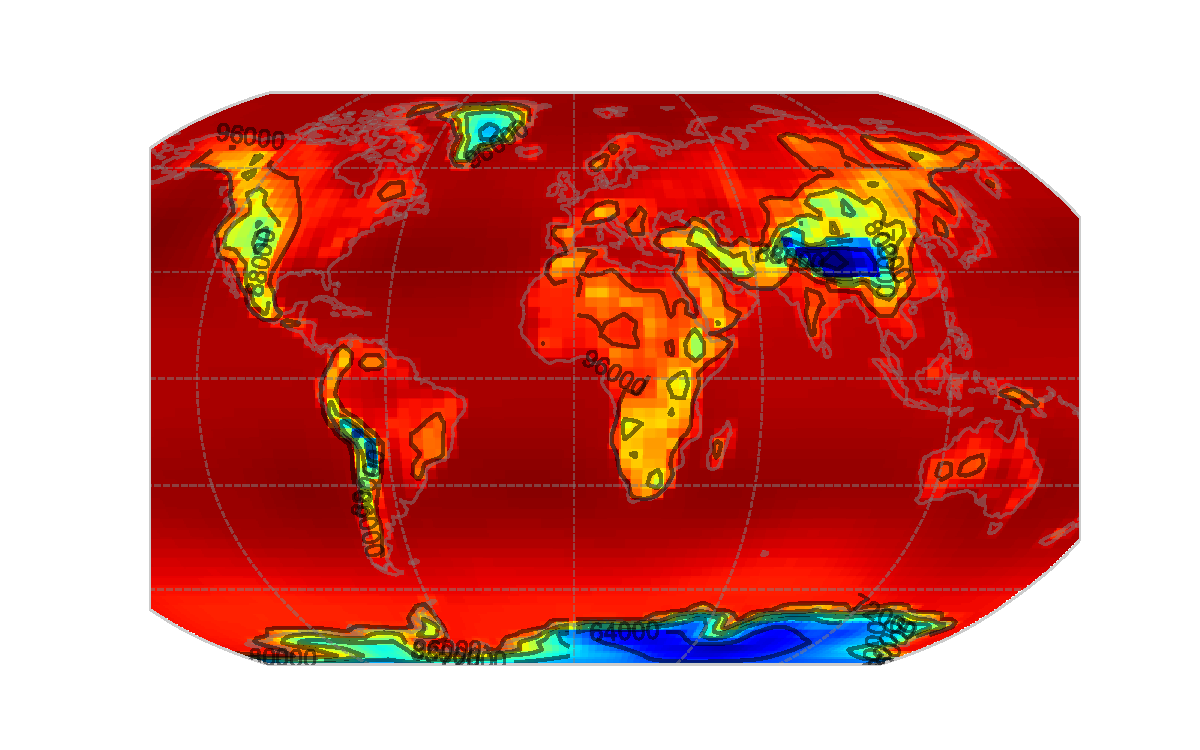
\includegraphics[width=\textwidth]{ftsm_res_ps_example_unob}
 		\caption{$Unobserved$}
 		\label{fig:ftsm_res_ps_unob}
 	\end{subfigure}             
 	\begin{subfigure}[b]{0.45\textwidth}
 		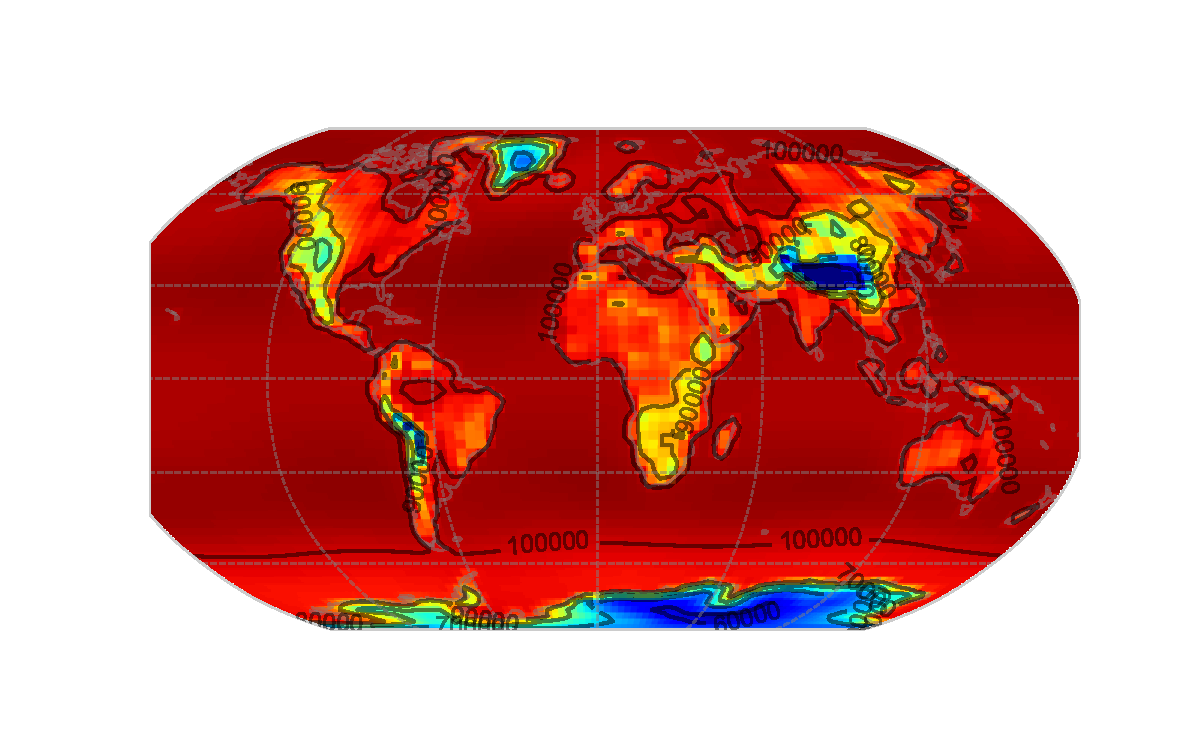
\includegraphics[width=\textwidth]{ftsm_res_ps_example_pace}
 		\caption{$PACE$}
 		\label{fig:ftsm_res_ps_pace}
 	\end{subfigure}
 	\vfill       
 	\begin{subfigure}[b]{0.45\textwidth}
 		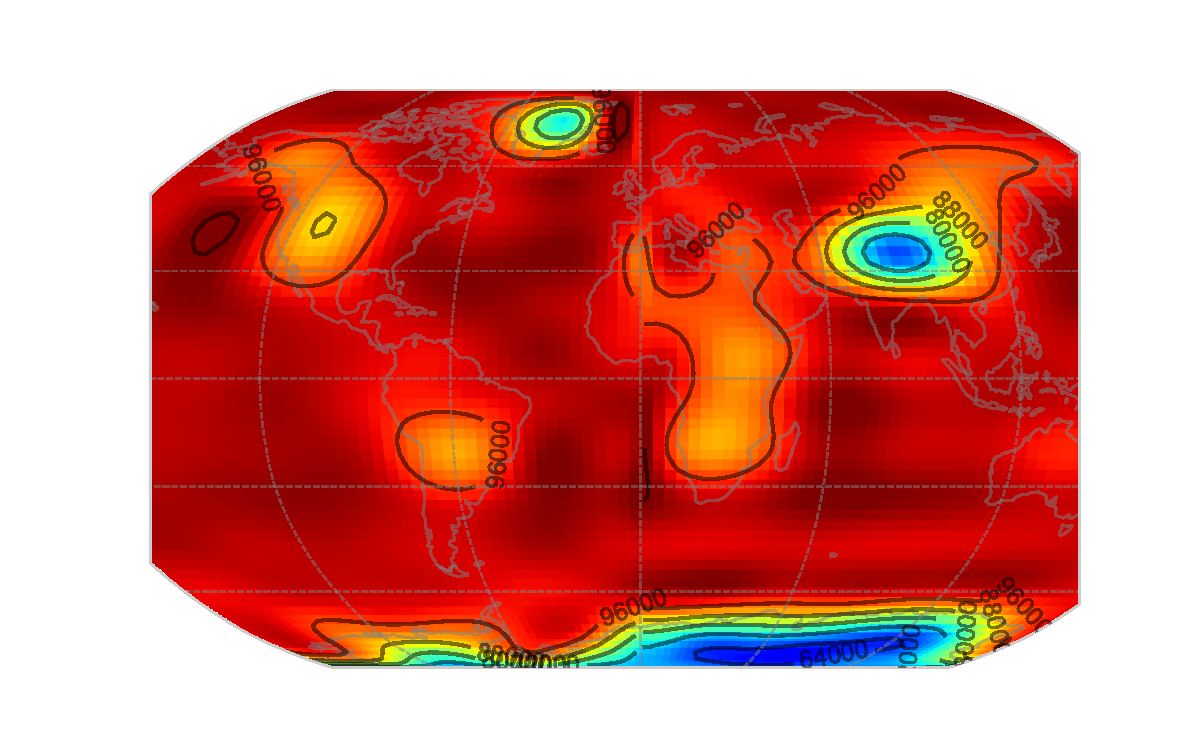
\includegraphics[width=\textwidth]{ftsm_res_ps_example_fpca}
 		\caption{$FPCA$}
 		\label{fig:ftsm_res_ps_fpca}
 	\end{subfigure}
 	\begin{subfigure}[b]{0.45\textwidth}
 		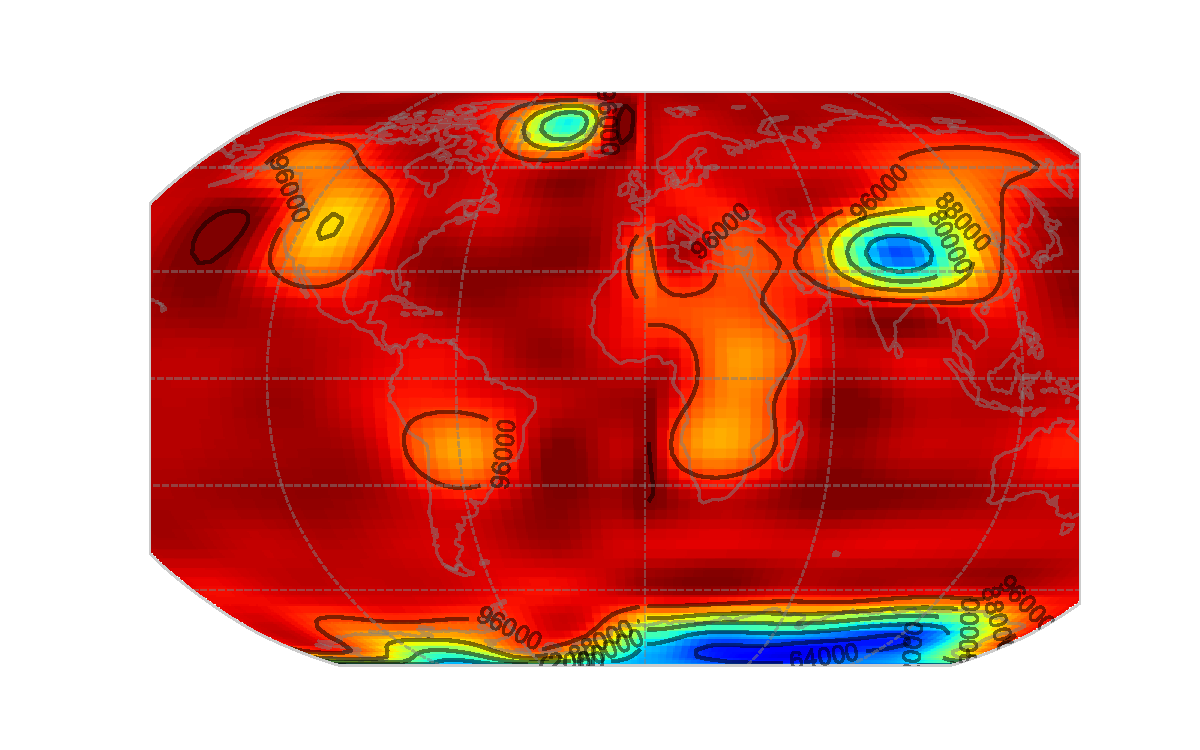
\includegraphics[width=\textwidth]{ftsm_res_ps_example_mafr}
 		\caption{$MAFR$}
 		\label{fig:ftsm_res_ps_mafr}
 	\end{subfigure}  
 	\caption[Example of the reconstruction ability of the various models for the PS atmospheric variable component of the CESM-LE dataset.]{Example of the reconstruction ability of the various models for the PS atmospheric variable component of the CESM-LE dataset. Notice how the FPCA and MAFR models miss the small scale spatial variation present in the unobserved surface. They have particular issue in recreating the abrupt changes at the sea-land boundary.}
 	\label{fig:ftsm_res_ps}
 \end{figure}

The forecasting results, given in Table~\ref{tab:ftsm_eo_for}, show similar results.
However, here we see the increasing impact of the FPCA and MAFR models. 
Especially in the atmospheric variables of TMQ and TREFHT we see an advantage in using the FPCA and MAFR models.
Here we see, slightly inverse to the interpolation results, that although the PACE model can deal with small scale spatial variation it struggles to model coherence through time using the spline extrapolation.
Whereas the FPCA and MAFR models produce score processes which can evidently be more easily forecast using the Gaussian process methodology outlined in Section~\ref{sec:ftsm_forecast}.
Additionally, we see that the RMSE and MAE metrics get worse for the PACE methodology as $h$ increases, whereas the FPCA and MAFR methodologies are more consistent for larger forecasting steps.
Again, we see little difference between the FPCA and MAFR models in both the interpolation and forecasting objectives. 

\section{Summary \label{sec:ftsm_summary}}
In this chapter we have considered a model for EO datasets based on the FTSM technique discussed in Section~\ref{sec:fts}.
We have considered, relatively uniquely, the idea that we consider our dataset as a time series of surfaces over our spatial domain and use the functional time series methodology discussed by \citep{hyndman_forecasting_2009} to provide an elegant way to forecast such datasets.
We have also considered a rotation to such models which, as discussed in Section~\ref{ssec:mafr}, may perhaps promote better forecasting ability.
This is compared against standard techniques that treat the data as a collection of independent functions over time, with each function corresponding to a spatial location. 


We have seen in Section~\ref{ssec:ftsm_sim_res} that on simulated datasets this technique works well.
We have compared these techniques under a variety of noise processes, including spatially structured noise which is often more realistic than independent noise processes in EO data.
We find, on the whole, they work at least equally well as the standard methodology which ignores spatial dependency between observations for interpolation, and outperforms this technique when forecasting.

However, on the CESM-LE data this technique falls down due to its difficulty in recreating small spatial scale variation.
As discussed in Section~\ref{ssec:ftsm_eo_disc}, this is due to our smoothing methodology to represent each observed surface using B-spline basis functions.
Given ample computation time this can be relieved by extending the dimension of this basis system.
However this is not always possible, and represents a real limitation of such methodologies.

A final advantage of such FTSM techniques for EO data is their ability to reduce the dataset dimension by introducing functional principal components which have a spatial domain.
These components can help to inform about modes of variation that are occurring over space.
Such dissections of the data can be useful in understanding the processes under examination. 
For example, Figure~\ref{fig:ftsm_res_TREFHT_fpc} gives the first three components for the TREFHT atmospheric variable of the CESM-LE dataset.
We can see clearly how the first corresponds to large scale variation between regions in the northern hemisphere whilst the second contains more localised areas of variation. 
We have further seen how the MAFR rotation can help to promote smooth functional principal components which may aide interpretability. 
Another example,which shows similar results for the pressure variable is given in Figure~\ref{fig:ftsm_res_PS_fpc}.
Here, one can see clearly how the first component focuses on various regions across the globe excluding the poles, whereas the second and third components focus mainly on the polar regions.

\begin{figure}
	\centering
	\begin{subfigure}[b]{0.45\textwidth}
		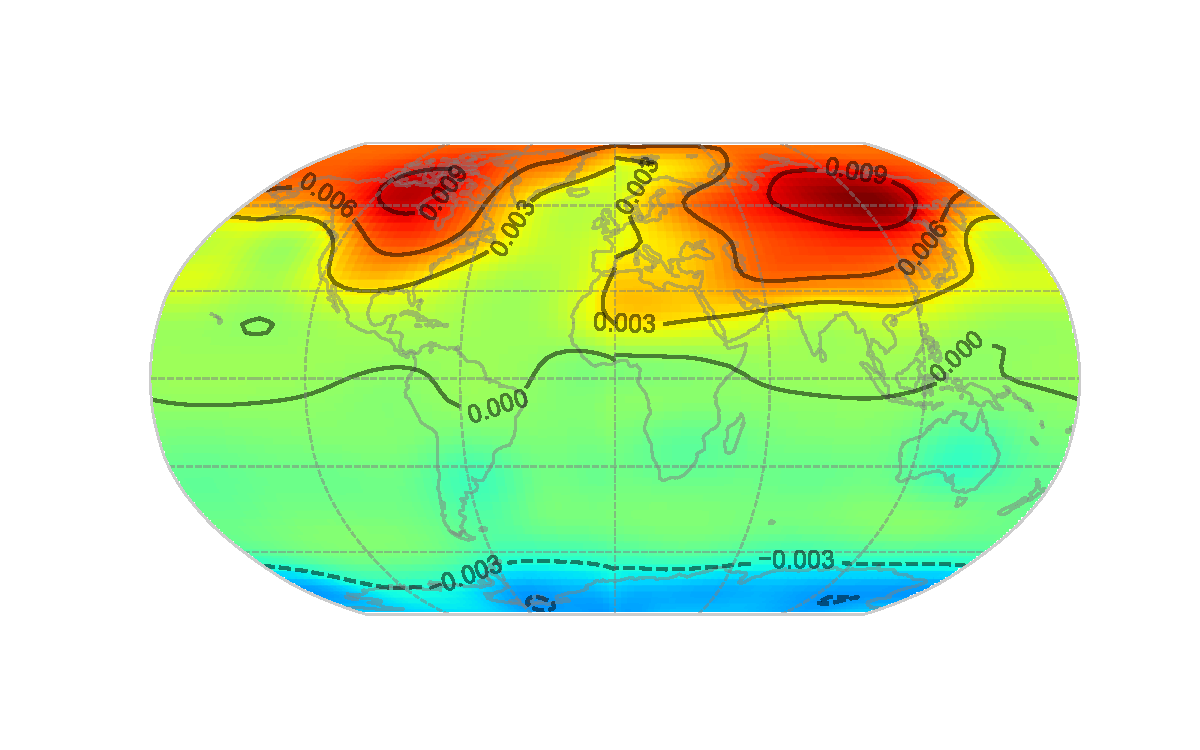
\includegraphics[width=\textwidth]{ftsm_res_TREFHT_fpc_0}
		\caption{$\vesub{\bar{\phi}}{1}$}
		\label{fig:ftsm_res_TREFHT_fpc_1}
	\end{subfigure}
	\vfill       
	\begin{subfigure}[b]{0.45\textwidth}
		\includegraphics[width=\textwidth]{ftsm_res_TREFHT_fpc_1}
		\caption{$\vesub{\bar{\phi}}{2}$}
		\label{fig:ftsm_res_TREFHT_fpc_2}
	\end{subfigure}
	\begin{subfigure}[b]{0.45\textwidth}
		\includegraphics[width=\textwidth]{ftsm_res_TREFHT_fpc_2}
		\caption{$\vesub{\bar{\phi}}{3}$}
		\label{fig:ftsm_res_TREFHT_fpc_3}
	\end{subfigure}
	\caption[Example of the functional principal components generated by the FPCA model with the TREFHT variable of the CESM-LE dataset.]{Example of the functional principal components generated by the FPCA model with the TREFHT variable of the CESM-LE dataset. Notice how each component shows a different mode of spatial variation present in the process. Such decompositions like these can be useful to understanding the process as a whole.}
	\label{fig:ftsm_res_TREFHT_fpc}
\end{figure}

\begin{figure}
	\centering
	\begin{subfigure}[b]{0.45\textwidth}
		\includegraphics[width=\textwidth]{ftsm_res_PS_fpc_0}
		\caption{$\vesub{\bar{\phi}}{1}$}
		\label{fig:ftsm_res_PS_fpc_1}
	\end{subfigure}
	\vfill       
	\begin{subfigure}[b]{0.45\textwidth}
		\includegraphics[width=\textwidth]{ftsm_res_PS_fpc_1}
		\caption{$\vesub{\bar{\phi}}{2}$}
		\label{fig:ftsm_res_PS_fpc_2}
	\end{subfigure}
	\begin{subfigure}[b]{0.45\textwidth}
		\includegraphics[width=\textwidth]{ftsm_res_PS_fpc_2}
		\caption{$\vesub{\bar{\phi}}{3}$}
		\label{fig:ftsm_res_PS_fpc_3}
	\end{subfigure}
	\caption[Example of the functional principal components generated by the FPCA model with the PS variable.]{Example of the functional principal components generated by the FPCA model with the PS variable of the CESM-LE dataset. Notice how each component shows a different mode of spatial variation present in the process. Such decompositions like these can be useful to understanding the process as a whole.}
	\label{fig:ftsm_res_PS_fpc}
\end{figure}

The standard PACE methodology can be seen to do well on the real world EO dataset due to its ability to capture small scale variations.
This occurs essentially because we treat each spatial location independently.
However, we have seen from both the FPCA and MAFR models that incorporating spatial information can be useful in recovering unobserved surfaces.
Utilising spatial dependency also has the added benefit of helping to ignore unstructured noise processes. 
A combination of both methodologies may then be desirable; that is, to incorporate spatial information into the PACE model.
The challenge is then to do so in such a way that keeps the model performing well where there exists small scale spatial variation.
In the following chapters we consider such a model. 
%!TEX root = ../thesis.tex
%*******************************************************************************
%*********************************** Fifth Chapter *****************************
%*******************************************************************************

\chapter{Correlated Principal Analysis through Conditional Expectation \label{cha:cpace}}  %Title of the Fifth Chapter

\ifpdf
    \graphicspath{{Chapter5/Figs/Raster/}{Chapter5/Figs/PDF/}{Chapter5/Figs/}}
\else
    \graphicspath{{Chapter5/Figs/Vector/}{Chapter5/Figs/}}
\fi

The foray into modelling using the spatial dimensions as the functional dimension in Chapter~\ref{cha:ftsm} gave us two clear findings.
Firstly, that spatial information is often useful in reconstruction and ignoring the spatial correlation observed between functional observations is throwing away information.
Secondly, smoothing across the spatial dimension can be problematic since it is incredibly easy to over smooth and lose important spatial details in the reconstructions. 
We note from Chapter~\ref{cha:ftsm} that the standard model, using time as the functional domain, managed to capture high levels of spatial detail since it treats each function as independent.
The downside to this model is that unobserved spatial locations cannot be reconstructed as we have no information about how to interpolate between functional observations.
One natural way to consider modelling such functional data is then to extend this model but to explicitly include the correlation between the observations in the model. 
We discuss these models in this chapter, we start with a discussion on models where the correlation between functional observations is purely spatial.

\section{Spatially Correlated Functional Data, \label{sec:space}}
The CESM-LE data set, as described in Chapter~\ref{cha:data}, provides a perfect example of spatially correlated functional data.
Take Figure~\ref{fig:cesm-space} for example, which shows the functional observations of the reference height temperature at 6 locations; the United Kingdom (UK), Ireland (IE), France (FR), Colombia (CO), Venezuela (VE), and Ecuador (EC). 

 \begin{figure}[htbp!] 
	\centering    
	\includegraphics[width=1.0\textwidth]{TREFHT_example_space_temp}
	\caption[CESM example of spatial correlation]{Example of functional observations reference height temperature across the globe from the CESM-LE data set. Notice that clearly locations close to each other in the globe tend to have more similar structure.}
	\label{fig:cesm-space}
\end{figure}
Clearly we can see locations in a similar vicinity having similar temperature patterns.
The European countries have a much larger range and overall lower mean temperature than those of the South American countries.
However, there are some similarities between all countries, such as the periodic nature of the functions, which indicate that there is some share of information across even large spatial distances. 

Incorporating spatial information into the models such as PACE, described in Section~\ref{sec:pace}, is therefore a natural extension. 
One such approach to this has been considered by \citeauthor{liu_functional_2017} in \citep{liu_functional_2017}. 
We will describe their model below and use this as our basis for modification and expansion in our proposed model for correlated functional data.

\subsection{Spatial principal analysis through conditional expectation, \citep{liu_functional_2017}, \label{ssec:space}}
A natural way to incorporate spatial correlation in our functional observation from the PACE model is to adjust how we define the score processes in Equation~\eqref{eqn:fd_temporal_fpca}.
The PACE model, \citep{yao_functional_2005}, implicitly uses the fact that $\mathbb{E}\left(\xi_{ik} \xi_{jk}\right) = 0$ for $i \ne j$ and $k=1,2,\cdots,K$. 
The Spatial PACE model (SPACE), \citep{liu_functional_2017} explicitly incorporates a model for this covariance.
In particular they consider the following form:
\begin{equation}
	\text{Cov}\left(\xi_{ip}, \xi_{jq}\right) = \begin{cases}
		\lambda_k \rho_{ijk}\text{ for $p=q=k$.} \\
		0 \text{ otherwise.}
	\end{cases}
\label{eqn:space_score}
\end{equation}
where $0 \le i, j \le N$ index the functional realisation and $0 \le p, q \le K$ index the component.
The correlation is induced by specifying the form of $\rho_{ijk}$ which acts as a spatial correlation factor in \citep{liu_functional_2017}. 
As such, it is useful to explicitly describe the association by writing $\rho_{ijk} = \rho_{k} \left( \vesub{s}{i}, \vesub{s}{j} \right)$ where $\ve{s}$ is an element in the spatial domain $\mathcal{S}$ as discussed in Chapter~\ref{cha:Into}.
Often the correlation structure may have an assumed parametric form, in which case we write $\rho_k \left(\ve{s}, \ve{s}^\prime \right) = \rho_k \left(\ve{s}, \ve{s}^\prime; \ve{\theta} \right)$ where we collect any hyper parameters for the parametric form into $\ve{\theta}$.
The covariance between $\mathcal{X}_i$ and $\mathcal{X}_j$ can be found as:
\begin{equation}
	\text{Cov}\left(\mathcal{X}_i(t), \mathcal{X}_j(t^\prime)\right) = \vesup{\phi}{\transpose}(t)\Sigma\left( \vesub{\xi}{i}, \vesub{\xi}{j}\right)\ve{\phi}(t^\prime)
	\label{eqn:space_cov}
\end{equation}
where $\Sigma\left( \vesub{\xi}{i}, \vesub{\xi}{j}\right) = \text{Diag}\left(\lambda_1 \rho_1(\ve{s}_i, \ve{s}_j), \lambda_2 \rho_2(\ve{s}_i, \ve{s}_j), \cdots, \lambda_K \rho_K(\ve{s}_i, \ve{s}_j) \right)$ is the covariance of the score processes.
We note that if $\Sigma\left( \vesub{\xi}{i}, \vesub{\xi}{j}\right) = \text{Diag}\left(\lambda_1, \lambda_2, \cdots, \lambda_K \right) \delta_{ij}$ in Equation~\eqref{eqn:space_cov} then the SPACE model reduces to the PACE model and corresponds to independent realisations of $\mathcal{X}$.
\citeauthor{liu_functional_2017} then obtain the equivalent of Equation~\eqref{eqn:fpc_best} for spatially correlated functional data as:
\begin{equation}
	\check{\tilde{\ve{\xi}}} = \mathbb{E}\left(\tve{\xi} | \tve{Y}\right) = \ve{\Sigma} \left( \tve{\xi}, \tve{Y}\right) \ve{\Sigma}\left(\tve{Y}, \tve{Y} \right)^{-1} \left(\tve{Y} - \tve{\mu}\right)
	\label{eqn:space_zeta}
\end{equation}
where $\ve{\Sigma}\left( \tilde{\ve{\xi}}, \tilde{\ve{Y}}\right)$ represents the covariance between the vector of scores at the appropriate locations with the observed functional data.
Similarly , $\ve{\Sigma}\left( \tilde{\ve{Y}}, \tilde{\ve{Y}}\right)$ represents the covariance between the vector of observed functional data with itself.
We have used the $\tilde{\cdot}$ notation as in \citep{liu_functional_2017} to denote these vectors.
The breakdown of the various terms in Equation~\eqref{eqn:space_zeta} is given below and follows \citep{liu_functional_2017}:
\begin{align}
	\vesub{y}{i} &= \left(y_i(t_{i1}), y_i(t_{i2}), \cdots, y_i(t_{iJ_i}) \right)^\transpose \\
	\tilde{\ve{Y}} &= \left(\vesub{y}{1}, \vesub{y}{2}, \cdots, \vesub{y}{N}\right)^\transpose \\
	\vesub{\mu}{i} & =  \left(\mu_i(t_{i1}), \mu_i(t_{i2}), \cdots, \mu_i(t_{iJ_i}) \right)^\transpose \\
	\tilde{\ve{\mu}} &= \left(\vesub{\mu}{1}, \vesub{\mu}{2}, \cdots, \vesub{\mu}{N}\right)^\transpose \\
	\vesub{\xi}{i} &= \left(\xi_{i1}, \xi_{i2}, \cdots, \xi_{iK} \right)^\transpose \\
	\tilde{\ve{\xi}} &= \left(\vesub{\xi}{1}, \vesub{\xi}{2}, \cdots,  \vesub{\xi}{N}\right)^\transpose
\end{align}
Here we see the extension from PACE model to SPACE where we use all data from the various functional observations at separate locations to give the best linear unbiased predictors. 
This captures the correlation between functional observations induced by the spatial correlation in the $K$ score processes.
We can see the impact of the score processes more clearly if we rewrite Equation~\eqref{eqn:space_zeta} as in \citep{liu_functional_2017}. 
Equation~\eqref{eqn:space_zeta} can be rewritten in a form similar to Equation~\eqref{eqn:fpc_best} using the structure of $\mathcal{X}$.
\begin{equation}
	\check{\tilde{\ve{\xi}}} = \ve{\Sigma}\left(\tve{\xi}, \tve{\xi}\right) \tvesup{\phi}{\transpose} \left(\tve{\phi} \ve{\Sigma}\left(\tve{\xi}, \tve{\xi}\right) \tvesup{\phi}{\transpose} + \sigma_\varepsilon^2 \ve{1} \right)^{-1} \left(\tve{Y} - \tve{\mu}\right)
\end{equation}
where $ \ve{\Sigma}\left(\tve{\xi}, \tve{\xi}\right)$ is the covariance between the vector of score values at the appropriate locations. Due to the construction in the SPACE model this has a relatively nice form as:
\begin{equation}
	 \ve{\Sigma}\left(\tve{\xi}, \tve{\xi}\right) = \tve{\rho} \bullet \left(\vesub{1}{N \times N} \otimes \ve{\Lambda} \right)
	 \label{eqn:cov_score_space}
\end{equation}
where $\bullet$ represents the element wise multiplication of the two matrices, $\ve{\Lambda} = \text{diag}\left(\lambda_1, \lambda_2, \cdots, \lambda_K\right)$ is the diagonal matrix of eigenvalues, and we construct $\tve{\rho}$ as follows: 
\begin{align}
	\vesub{\rho}{ij} &= \text{Diag} \left( \rho_1(\vesub{s}{i}, \vesub{s}{j}), \rho_2(\vesub{s}{i}, \vesub{s}{j}), \cdots, \rho_K(\vesub{s}{i}, \vesub{s}{j}) \right) \\
	\tve{\rho} &= \left[\vesub{\rho}{ij}\right]
\end{align}
where $\left[\cdot_{ij}\right]$ represents a matrix with ${ij}^\text{th}$ entry being $\cdot_{ij}$.
As discussed in \citep{liu_functional_2017} the covariance of the score process $\ve{\Sigma}\left(\tve{\xi}, \tve{\xi}\right)$ can take a simpler form if we assume that the correlation structure across all components are the same. 
That is if $\rho_{ijk} = \rho_{ij} = \rho(\vesub{s}{i}, \vesub{s}{j}) $ for all $k=1, 2, \cdots, K$ we have the following form:
\begin{equation}
	\ve{\Sigma}\left(\tve{\xi}, \tve{\xi}\right) = \ve{\rho} \otimes \ve{\Lambda}
	\label{eqn:cov_score_space_separable}
\end{equation}
where $\ve{\rho} = \left[\rho_{ij}\right]$.
This is a particularly strong assumption which is unlikely to be observed in practice.

By substituting estimates for the various terms in Equation~\eqref{eqn:cov_score_space} the estimate of $\tve{\xi}$ is derived, namely: 

\begin{equation}
	\hat{\tve{\xi}} =   \hat{\ve{\Sigma}}\left(\tve{\xi}, \tve{\xi}\right) \hat{\tve{\phi}}^\transpose \left(\hat{\tve{\phi}} \hat{\ve{\Sigma}}\left(\tve{\xi}, \tve{\xi}\right) \hat{\tve{\phi}}^\transpose + \hat{\sigma}_\varepsilon^2 \ve{1} \right)^{-1} \left(\tve{Y} - \hat{\tve{\mu}}\right)
\end{equation}
where $\hat{\cdot}$ represents the estimate of $\cdot$.
In particular,  $\hat{\ve{\Sigma}}\left(\tve{\xi}, \tve{\xi}\right) = \hat{\tve{\rho}} \bullet \left(\ve{1}_{N \times N} \otimes \hat{\ve{\Lambda}}\right)$ is our estimated score covariance. 
This highlights the first significant change from the PACE methodology. 
As discussed in \citep{liu_functional_2017} the same estimation methodology as in PACE can be used to estimate the eigenfunctions, eigenvalues and noise variance.
See Chapter~\ref{cha:background} for details to these estimations under the PACE model.
There is some need to show that such estimators are consistent under spatially correlated data, which \citep{liu_functional_2017} show for locally linear smoothers and we shall show for spline smoothers in the following work. 
Ignoring this for the time being, the additional work under the SPACE model is the estimation of the correlation values that construct Equation~\eqref{eqn:cov_score_space}. 
In \citeauthor{liu_functional_2017} SPACE model these are estimated using the following approach.
For a more in depth discussion, we refer the reader to \citep{liu_functional_2017}.

Firstly, the construction of cross-covariances are required.
The cross-covariance, $G_{ij} = \text{Cov}\left(\mathcal{X}_i, \mathcal{X}_j\right)$, is the covariance between the $i^\text{th}$ and $j^\text{th}$  functional variable. 
This has the form given in Equation~\eqref{eqn:space_cov}. 
If we further assume $\rho_1(\vesub{s}{i}, \vesub{s}{j}) > \rho_2(\vesub{s}{i}, \vesub{s}{j}) > \cdots > \rho_K(\vesub{s}{i}, \vesub{s}{j})$ then the sequence $\{\vesub{\rho}{k}(\vesub{s}{i}, \vesub{s}{j})\}_{k=1}^K$ are eigenvalues of $G_{ij}$.
Therefore $\rho_{ijk}$ can be estimated as the ratio of the $k^\text{th}$ eigenvalue of cross-covariance $G_{ij}$ to the $k^\text{th}$ eigenvalue of the covariance $G$. 
That is:
\begin{equation}
	\hat{\rho}_{ijk} = \frac{\hat{\lambda}_k(\vesub{s}{i}, \vesub{s}{j})}{\hat{\lambda}_k}
\end{equation}
where $\hat{\lambda}_k(\vesub{s}{i}, \vesub{s}{j})$ is the $k^\text{th}$ eigenvalue estimate from the decomposition of cross covariance $G_{ij}$.
A series of empirical correlation factors $\hat{\rho}_{ijk}$ can then be used to estimate the hyper parameters in any parametric form of the correlation structure as needed. 
In \citep{liu_functional_2017} they use a quasi-Newton method (BFGS, \citep{fletcher_practical_1987}) to estimate hyper parameters by minimising the sum of squared differences between empirical and fitted correlations.

The SPACE model is shown to be effective, identifiable, and outperforms the PACE model in \citep{liu_functional_2017}.
In particular, it performs more accurate gap filling for unobserved trajectories on real world data sets.
These properties suggest it is a great framework to model spatially correlated functional data.
However we note some possible limitations of the model as proposed by \citep{liu_functional_2017}.
Firstly, the estimation procedure of the SPACE model for the score hyper parameters requires the forming of possibly numerous cross covariance surfaces.
These may become either computationally tiresome to compute as each needs smoothing and decomposing into its eigenvalues or there may be insufficient data to obtain an accurate representation of the true cross-covariance. 
Secondly, the SPACE and PACE models both require the need of estimating the score process values at the prediction location before then using this to reconstruct the unobserved trajectory.
This is a slightly convoluted approach as typically the score process is not what the end user needs but rather the full reconstruction is the useful quantity to estimate. 
Finally, \citep{liu_functional_2017} uses local linear smoothers for representing smooths for both the mean and covariance surfaces and proves asymptotic properties under this kind of linear smoother for estimation of these surfaces under spatially correlated functional data.
As discussed in Chapter~\ref{cha:background} we prefer the properties of spline smoothing as an approach.
To the authors knowledge there are no such asymptotic results for the mean and covariance smoothing under spatially correlated data using a regularised spline smoother. 

In the following section we provide a simple framework based on the SPACE model which provides a more flexible way to view and estimate such functional data.
We aim to overcome the limitation of estimating multiple cross-covariances and remove the need for the intermediate estimation of the score processes by considering the model in the context of a Gaussian process. 
We also show the asymptotic properties of using a spline smoother on correlated functional data in the processes.

\section{Correlated Principal Analysis through Conditional Expectation} 
To begin the extension to the SPACE model, discussed in Section~\ref{ssec:space}, we restrict ourselves to the notation that $\ve{s} \in \mathcal{S} \subset \mathbb{R}^2$ for simplicity.
In this case we are now considering as in the SPACE model to incorporate spatial correlation between observations. 
To do this we employ a similar model as in SPACE, however we view this using Gaussian processes.
In particular we will specify that each score process $\xi_k(\ve{s})$ be a Gaussian process.
In doing so we will generate a framework which we will argue constitutes a more efficient, flexible, and robust framework than is discussed in SPACE. 

Without further ado, we let $\xi_k$ be a zero mean Gaussian process, which we denote as:
\begin{align}
	\xi_k&: \mathcal{S} \to \mathbb{R} \\
	\xi_k &\sim \mathcal{GP}\left(0, a_k \right)
\end{align}
where $a_k: \mathcal{S} \times \mathcal{S} \to \mathbb{R} $ is the kernel function of the $k^\text{th}$ Gaussian process. 
This kernel function is responsible for determining the spatial correlation of our functional random variables. 
In fact, we can assume without loss of generality that the variance of this kernel function is $\lambda_k$.
Therefore, we  actually only need to specify a correlation function which will determine the correlation of our functional random variable. 
We also follow the convention of \citep{liu_functional_2017} and specify that the cross covariance between the $K$ Gaussian process is zero.
That is:
\begin{equation}
	\text{Cov}\left(\xi_p, \xi_q\right) = \begin{cases}
		a_k \text{ if p=q} \\
		0 \text{ otherwise}
	\end{cases}
	\label{eqn:cpace_score}
\end{equation}
We note that this is equivalent to the SPACE model  if $a_k(\ve{s}, \vesup{s}{\prime})  = \lambda_k \rho_k(\ve{s}, \vesup{s}{\prime})$ which follows from equating Equation~\eqref{eqn:cpace_score} and Equation~\eqref{eqn:space_score}.
With such a framework for the score processes we can now look back at the whole process of generating the functional random variable $\mathcal{X}$ with the Gaussian process in mind and including the spatial coordinate as a parameter rather than an index.
\begin{equation}
	\mathcal{X}\left(\ve{s}, t \right) = \mu(t) + \sum_{k=1}^K \xi_k(\ve{s}) \phi_k(t)
	\label{eqn:fpca_cpace}
\end{equation}
where we now consider $\xi_k$ to be a Gaussian process over the spatial domain $\mathcal{S}$.
Using this structure for $\mathcal{X}$ we can view $\mathcal{X}$ as being drawn from a larger Gaussian process. 
\begin{align}
	\mathcal{X}&: \mathcal{S} \times \mathcal{T} \to \mathbb{R}\\
	\mathcal{X} &\sim \mathcal{GP}\left(\mu, a_\mathcal{X}\right)
\end{align}
where we can construct $a_\mathcal{X}: \mathcal{S}^2 \times \mathcal{T}^2 \to \mathbb{R}$ ,the kernel function, as follows: 
\begin{equation}
	a_\mathcal{X}\left( \ve{s}, t, \vesup{s}{\prime}, t^\prime \right) = \vesup{\phi}{\transpose}(t)\text{Diag}\left(a_1(\ve{s}, \vesup{s}{\prime}), a_2(\ve{s}, \vesup{s}{\prime}), \cdots, a_K(\ve{s}, \vesup{s}{\prime}) \right) \ve{\phi}(t^\prime)
	\label{eqn:cpace_k_fn_form}
\end{equation}
and $\ve{\phi}(t) = \left(\phi_1(t), \phi_2(t), \cdots, \phi_K(t)\right)^\transpose$ is the $K$ length vector of eigenfunctions evaluated at $t$.
The mean function $\mu$ remains the same mean function as discussed in the SPACE and PACE models.
There is possible scope to extend this mean function to be over spatial domain as well as the temporal domain but we will focus on a mean function which is constant over the space.
The kernel function $a_\mathcal{X}$ is a structured kernel comprising of the $K$ eigenfunctions of $\mathcal{X}$ and the $K$ score parametric kernel functions.
As such we can view the kernel as having essentially $K$ lots of hyper parameters, $\{\vesub{\theta}{k}\}_{k=1}^K$ that will need estimation to determine the parametric score kernel functions.
In addition to this we need to estimate the $K$ eigenfunctions and the mean function. 
In the following section we discuss the estimation of the mean function.

The discussion of the estimation of the eigenfunctions and hyper parameters are found in Sections~\ref{sec:cpace_eigen_estim},~\ref{sec:cpace_score_estim} respectively.

\section{Mean function estimation \label{sec:cpace_mean_estim}}.
We consider the estimation of the mean function $\mu$ under correlated sparse functional data.
The data model is as given by Equation~\eqref{eqn:fd_temporal}.
As described in Chapter~\ref{cha:background} for independently observed functional data \citep{yao_functional_2005} have shown the asymptotic properties for an estimator of the mean function using a local linear smoother.
For spatially correlated functional data these results were extended in \citep{liu_functional_2017} using the same locally linear smoothing techniques.
However, as mentioned in Chapter~\ref{cha:background}, in our work we will focus on the use of regularised spline smoothing as our smoothing technique for estimation. 
In the following we consider an estimation technique for the mean function using regularised spline smoothing under correlated functional observations.

We approximate the mean function $\mu(t)$ by the spline function $\vess{c}{\mu}{\transpose} \vess{B}{d}{\ve{\tau}}(t) $ where, as discussed in Section~\ref{sec:splines}, $\vess{B}{\tau}{d}(t) = \left(B_{d,1}^{\ve{\tau}}(t), B_{d,2}^{\ve{\tau}}(t), \cdots, B_{d,K_\mu}^{\ve{\tau}}(t)\right)$ is the $K_\mu$ length collection of B-splines of order $d$ with knot vector $\ve{\tau}$.
The estimate for the coefficient vector $\vesub{c}{\mu}$ is found as:
\begin{equation}
	\vesub{\hat{c}}{\mu} = \argmin_{\ve{c}} \left[\sum_{i=1}^N \sum_{j=1}^{J_i} w_i \{ y_i(t_{ij}) - \vesup{c}{\transpose} \vess{B}{d}{\ve{\tau}} (t_{ij}) \}^2 + \omega \vesup{c}{\transpose} \ve{P} \ve{c} \right]
	\label{eqn:mean_coefs}
\end{equation}
where $w_i$ are fixed weights to be specified and satisfy $\sum_{i=1}^{N} J_i w_i = 1$, the $q^\text{th}$ order penalty matrix $\ve{P} \in \mathbb{R}^{K_\mu \times K_\mu}$ is positive semi-definite and to be specified, and $\omega$ is a smoothing parameter which balances the data fit and smoothness of the fitted mean function. 
The form of this penalised spline regression with the various components is discussed in general in Section~\ref{sec:splines}. 

We follow \citep{xiao_asymptotic_2020} and introduce some more notation corresponding to the above which will be advantageous for further results.
Let $\vesub{B}{i} = \left[\vess{B}{d}{\ve{\tau}} (t_{i1}), \vess{B}{d}{\ve{\tau}} (t_{i2}), \cdots, \vess{B}{d}{\ve{\tau}} (t_{iJ_i})\right]^\transpose \in \mathbb{R}^{J_i \times K_\mu}$ where we drop the notation for the order and knot vector and treat these as to be specified and fixed.
Let $\ve{Y} = \left[\vess{y}{1}{\transpose}, \vess{y}{2}{\transpose}, \cdots, \vess{y}{N}{\transpose}\right]^\transpose$ and $\ve{B} = \left[\vess{B}{1}{\transpose}, \vess{B}{2}{\transpose}, \cdots, \vess{B}{N}{\transpose}\right]^\transpose$.
Similarly, let $\vesub{W}{i} = w_i \ve{I}_{J_i \times J_i}$ and $\ve{W} = \text{BlockDiag}\left(\vesub{W}{1}, \vesub{W}{2}, \cdots, \vesub{W}{N}\right)$.
Then $\vesub{\hat{c}}{\mu} = \vess{H}{N}{-1} \left( \vesup{B}{\transpose}\ve{W}\ve{Y}\right)$ where $\vesub{H}{N} = \vesub{G}{N} + \omega \ve{P}$ and $\vesub{G}{N} = \vesup{B}{\transpose} \ve{W} \ve{B}$. The mean function estimator is then given by:
\begin{equation}
	\hat{\mu}(t) = \vess{\hat{c}}{\mu}{\transpose}\vess{B}{d}{\ve{\tau}}(t)
\end{equation} 

Using the above notation we now establish the asymptotic properties of the mean function estimator, $\hat{\mu}(t)$. 
The majority of this theorem and proof follows a similar theorem proposed by \citeauthor{xiao_asymptotic_2020} in \citep{xiao_asymptotic_2020}.
They propose the asymptotic properties of a penalised spline smoother for independently observed functional data, \citep{xiao_asymptotic_2020}.
We extend these results to the case where we have dependently observed functional data.
To facilitate this section we introduce some notation on norms, this notation is consistent with \citep{xiao_asymptotic_2020}. 
As usual let $\lVert \cdot \rVert_2$ denote the Euclidean norm, $\lVert \cdot \rVert_{F}$ denote the Frobenius norm, and $\lVert \cdot \rVert_\text{op}$ denote the operator norm.
For a matrix $\ve{A} = \left[a_{ij}\right]$, let $\lVert \ve{A} \rVert_\text{max} = \max_{i,j} \lvert a_{ij} \rvert$ and $\lVert \ve{A} \rVert_\infty = \max_i \sum_j \lvert a_{ij} \rvert$.
For a univariate continuous function $g$ over $\mathcal{T}$ we denote the supreme norm as $\lVert g \rVert$.
The $L_2$ norm of $g$ is denoted by $\lVert g \rVert_{L_2}$.
Finally, for every positive integer $p$, denote the class of functions with continuous $p^\text{th}$ derivative over $\mathcal{T}$ by $\mathcal{C}^p(\mathcal{T})$.

First we make the following assumptions required for the properties. 
We proceed with assumptions similar to \citep{xiao_asymptotic_2020}. 
\begin{assumption}
	(a) The random functions $\mathcal{X}_i$ are identically distributed according to $\mathcal{X}$. (b) The random errors $\varepsilon_{ij}$ are independent of the random functions $\mathcal{X}_i$ and are independent and identically distributed with mean zero and variance $\sigma_\varepsilon < \infty$. (c) We have a finite cross covariance function, $\lVert a_\mathcal{X}\rVert < \infty$. 
	\label{ass:1}
\end{assumption}

\begin{assumption}
	(a) The number of basis functions $K_\mu$ satisfies $K_\mu \geq N^{\delta_1}$ for some constant $\delta_1 > 0$ and $K_\mu = o(N)$. (b) The smoothing parameter  $\omega$ satisfies $\omega = o(N^{-\delta_2})$ for some constant $\delta_2$. 
	\label{ass:2}
\end{assumption}

We then assume we have a fixed common design, as suggested by \citep{xiao_asymptotic_2020}. In this case we suppose each functional data is observed at the same fixed set of time points. This observational design is made explicit using Assumption~\ref{ass:3}. 

\begin{assumption}
	(a) $J_i = J$ for all $i$ and $t_{ij} = \frac{j-\frac{1}{2}}{J}$. (b) $J \geq N^{\delta_3}$ for some constant $\delta_3 > 0$. (c) There exists a sufficiently small constant $c_0 > 0$ such that $K_\mu \leq c_0 J$.
	\label{ass:3}
\end{assumption}

Under Assumptions~\ref{ass:1}-~\ref{ass:3} we then state our result for the $L_2$ convergence of the mean function estimator from correlated functional data under fixed common design conditions. 

\begin{theorem}[Mean function: $L_2$ convergence under fixed common design]
	Suppose that Assumptions~\ref{ass:1}-~\ref{ass:3} hold. Let $h = K_\mu^{-1}$, $h_e = \max\{h, \omega^{\frac{1}{2d}}\}$, $\tau_1 = \sum_{i=1}^{N} J w_i^2$, $\tau_2 = \sum_{i=1}^{N}J(J -1) w_i^2$, and $\tau_3 = \sum_{i=1}^N \sum_{\substack{j=1 \\ i \ne j}}^N w_i w_j J^2 a_{ij}^*$ where $a_{ij}^* = \max_{j1, j2} \lvert a_\mathcal{X}\left(\vesub{s}{i}, t_{ij_1}, \vesub{s}{j}, t_{jj_2}\right) \rvert$. 
	
	If $\mu \in \mathcal{C}^p\left( \mathcal{T} \right)$ with $q \leq \min(p, d+1)$, then:
	\begin{equation*}
		\mathbb{E}\left[ \lVert \hat{\mu} - \mu \rVert_{L_2}^2 \right] = O\left( h^{2(d+1)} \right) + o(h^{2p}) + O\left( \omega^2 h_e^{-2q} \right) + O\left( \tau_1 h_e^{-1}+ \tau_2 + \tau_3\right)
	\end{equation*}
	\label{thm:cpace_mean}
\end{theorem}

As mentioned in \citep{xiao_asymptotic_2020} the term $O\left( h^{2(d+1)} \right) + o(h^{2p})$ is the order of the integrated and squared approximation bias of the spline function, the term $O\left( \omega^2 h_e^{-2q} \right)$ is the order of the integrated and squared shrinkage bias from the smoothness penalty, and the final term $ O\left( \tau_1 h_e^{-1}+ \tau_2 + \tau_3\right)$ is the integrated variability of the penalised splines. 
In particular, the $O(\tau_2)$ term corresponds to within subject correlation and the $O(\tau_3)$ term to the between subject correlation. 
The above theorem holds for general weights $w_i$, however a popular choice for such weights is equally weighted observations and setting $w_i = (NJ)^{-1}$. 
In this case $\tau_1 = (NJ)^{-1}$, $\tau_2 = N^{-1} - \tau_1$, and $\tau_3 = \frac{1}{N^2}\sum_{i=1}^N \sum_{j=1}^N a_{ij}^*$. 
Thus with additional constraints on the correlation $a_\mathcal{X}$ we can ensure that the variance of the penalised splines can remain, like in the independent case, $O(N^{-1})$.
One such simple requirement would be, like in the SPACE model, \citep{liu_functional_2017}, that:
\begin{equation}
	\frac{1}{N^2}\sum_{i=1}^N \sum_{j=1}^N \lvert a_\mathcal{X}(\vesub{s}{i}, t, \vesub{s}{j}, t^\prime) \rvert \to 0 \text{ as } N \to \infty
\end{equation}
for any $t, t^\prime \in \mathcal{T}$.
This essentially requires the correlation between observations to decay sufficiently fast so that the average correlation across all observation pairs becomes negligible as the number of observations tends to infinity.

\subsection{\label{ssec:proof_mean_estim}Proof of Theorem~\ref{thm:cpace_mean}}
We first state and prove some technical lemmas which will aid in the proof of Theorem~\ref{thm:cpace_mean}.
These lemmas are presented and discussed in more detail in \citep{xiao_asymptotic_2020} and the references within.
We state these here without proof for completeness. 

\begin{lemma}
	Suppose that Assumption~\ref{ass:2} (a) holds. If $\mu \in \mathcal{C}^P\left(\mathcal{T}\right)$, then there exists a spline function $\nu_\mu \left(t\right) = \vesup{\beta}{\transpose} \ve{B}(t)$ for some $\ve{\beta} \in \mathbb{R}^{K_\mu}$ such that: 
	\begin{equation}
		\lVert \mu^{(i)}- \nu_\mu^{(i)} \rVert = O\left( h^{d+1-i} \right) + o(h^{p-i})
	\end{equation}
\label{lem:1}
\end{lemma}

As in \citep{xiao_asymptotic_2020} we use notation for describing the design points.
Let $Q_N(t) = \sum_{i=1}^{N} w_i \sum_{j=1}^{J_i} 1_{t_{ij} < t}$ where $1_{\cdot}$ is an indicator function.
The function $Q_N(t)$ is an empirical cumulative distribution function under the fixed common design.
Let $Q(t) = t$ be the cumulative distribution function under fixed common design with density $\rho(t)=1$.
It will be shown that such an empirical cumulative distribution function $Q_N$ converges to $Q$ in the following lemmas, we refer to \citep{xiao_asymptotic_2020} for proofs of these lemmas.
\begin{lemma}
	Suppose that Assumption~\ref{ass:2} (a) holds and $p \ge 1$.
	Let $\nu_mu$ be the spline function described in Lemma~\ref{lem:1} and $F\left(\cdot\right)$ be a cumulative distribution function in $\mathcal{T}$.
	Then for $i=0$ or $i=1$: 
	\begin{equation}
		\max_k \lvert \int B_k(t) \{\mu^{(i)} - \nu_\mu^{(i)}\} dF(t)\rvert = o\left(h^{p+1-i}\right) + o\left(h^{p-i} \lVert F - Q \rVert \right)
	\end{equation}
	\label{lem:2}
\end{lemma}
Lemma~\ref{lem:2} is given as Lemma A.2 in \citep{xiao_asymptotic_2020} which shows the same lemma in a more general sense.
The following lemmas apply under the fixed common design setting so we assume Assumption~\ref{ass:3} holds for each. 
Let $\ve{G} = \int \ve{B}\left(s\right) \vesup{B}{\transpose}\left(s\right) ds$.
\begin{lemma}
	Suppose that Assumption~\ref{ass:2} and Assumption~\ref{ass:3} hold.
	Then:
	\begin{equation} 
		\vesub{G}{N} \simeq \ve{G} \simeq h \ve{I}
	\end{equation}
\label{lem:3}
\end{lemma}

\begin{lemma}
	Suppose that Assumption~\ref{ass:2} and Assumption~\ref{ass:3} hold.
	Let $\alpha_{ij}$ represent the $(i, j)^\text{th}$ element of $\vess{G}{N}{-1}$.
	Then there exists constants $c \ge 0$ and $0 < \gamma < 1$ such that, for large N:
	\begin{equation}
		\lvert \alpha_{ij} \rvert  \leq c h^{-1} \gamma^{\lvert i - j \rvert}
	\end{equation}
	In addition, 
	\begin{equation}
		\lVert \vess{G}{N}{-1} \rVert_{\infty} = O\left(h^{-1}\right)
	\end{equation}
	\label{lem:4}
\end{lemma}

\begin{lemma}
	Suppose that Assumption~\ref{ass:2} and Assumption~\ref{ass:3} hold.	
	Then, the following hold: 
	\begin{eqnarray}
		\lVert \vesub{G}{N} - \ve{G} \rVert_{\text{max}} &=& O\left(\lVert Q_N - Q \rVert_{\text{max}}\right) \\
		\lVert \vess{G}{N}{-1} - \vesup{G}{-1} \rVert_{\text{max}} &=& O\left(h^{-2}\lVert Q_N - Q \rVert_{\text{max}}\right) \\
		\lVert \vess{G}{N}{-1} - \vesup{G}{-1} \rVert_{\infty} &=& O\left(h^{-2}\lVert Q_N - Q \rVert_{\text{max}}\right) 
	\end{eqnarray}
	\label{lem:5}
\end{lemma}

Lemmas~\ref{lem:3},~\ref{lem:4},~\ref{lem:5} cause the following to hold under fixed common design, as shown in \citep{xiao_asymptotic_2020}:
\begin{lemma}
	Suppose that Assumption~\ref{ass:2} and Assumption~\ref{ass:3} hold.
	Define $\ve{\gamma} = \vess{G}{N}{-1} \left(\vesup{B}{\transpose} \ve{W} \ve{\mu}\right)$ where $\ve{\mu} = \left[\vess{\mu}{1}{\transpose}, \vess{\mu}{2}{\transpose}, \cdots, \vess{\mu}{N}{\transpose}\right]^\transpose$ and $\vesub{\mu}{i} = \left(\mu(t_{i1}), \mu(t_{i2}), \cdots, \mu(t_{iJ_i})\right)^\transpose$. 
	Then the following equalities hold:
	\begin{eqnarray}
		\lVert \vess{H}{N}{-1} \rVert_{\text{max}} &=& O\left(h_e^{-1}\right) \\
		\lVert \vess{H}{N}{-1} \rVert_{\infty} &=& O\left(h^{-1}\right) \\
		\lVert \vess{H}{N}{-1} \ve{P} \ve{\gamma} \rVert_{\text{max}} &=& O\left(h_e^{-q}\right)
	\end{eqnarray}
	\label{lem:6}
\end{lemma}

Using the above Lemma~\ref{lem:1}-~\ref{lem:6} we can now prove the asymptotic properties described in Theorem~\ref{thm:cpace_mean} under fixed design conditions.

\begin{proof}[Proof of Theorem~\ref{thm:cpace_mean}]
	The proof of the asymptotic properties of the mean estimator using a penalised spline estimator under dependently observed functional data follows closely the proof of the mean estimator using a penalised spline under independent observed functional data given in \citep{xiao_asymptotic_2020}.
	As a matter of completeness we will present the full proof, although much is the same as presented in \citep{xiao_asymptotic_2020} due to the similar nature of the theorems.
	Deviations from the proof in \citep{xiao_asymptotic_2020} are due to the fact we can no longer assume independent observations as is done in \citep{xiao_asymptotic_2020}.
	These will be clearly signposted. 
	
	First, without loss of generality, let $\mathcal{T} = \left[0, 1\right]$.
	Then:
	\begin{equation}
		\mathbb{E} \left(\lVert \hat{\mu} - \mu \rVert_{L_2}^2 \right) \leq \lVert \mathbb{E}\left( \left(\hat{\mu} - \mu \right)^2 \right) \rVert \leq \lVert \mathbb{E}\left(\hat{\mu}\right) - \mu \rVert + \lVert \text{var}\left(\hat{\mu}\right)\rVert
		\label{eqn:bias_var_thm}
	\end{equation}
where the first term in the right hand side of Equation~\eqref{eqn:bias_var_thm} corresponds to a bias term and the second being the variance term.
We bound the bias and variance terms separately.
We start with the bias term. 

The bound on the bias term is derived exactly as in \citep{xiao_asymptotic_2020}. 
First, let $\nu_\mu$ be the spline function as defined in Lemma~\ref{lem:1} such that: 
\begin{equation}
		\lVert \mu - \nu_\mu \rVert = O\left( h^{d+1} \right) + o(h^{p})
		\label{eqn:cpace_mu_nu_bound}
\end{equation}

Define $\vesub{\nu}{i, \mu} = \left(\nu_\mu(t_{i1}), \nu_\mu(t_{i2}), \cdots, \nu_\mu(t_{iJ_i})\right)^\transpose$ and $\vesub{\nu}{\mu} = \left[\vess{\nu}{1, \mu}{\transpose}, \vess{\nu}{2, \mu}{\transpose}, \cdots, \vess{\nu}{N, \mu}{\transpose} \right]^\transpose$. 
Then we can write: 
\begin{eqnarray}
	\mathbb{E}\left(\hat{\mu}\right) &=& \vesup{B}{\transpose}(t)\vess{H}{N}{-1}\left(\vesup{B}{\transpose} \ve{W} \ve{\mu} \right) \\
	&=& \vesup{B}{\transpose}(t)\vess{G}{N}{-1}\left(\vesup{B}{\transpose} \ve{W} \ve{\mu} \right) - \vesup{B}{\transpose}(t)\vess{H}{N}{-1} \left(\omega \ve{P}\right)\vess{G}{N}{-1}\left(\vesup{B}{\transpose} \ve{W} \ve{\mu} \right)
	\label{eqn:bias_split}
\end{eqnarray}
Splitting the first term in Equation~\eqref{eqn:bias_split} using our spline function $\vesub{\nu}{\mu}$ we can write:
\begin{equation}
	\begin{split}
		\mathbb{E}\left(\hat{\mu}\right)  &= \vesup{B}{\transpose}(t)\vess{G}{N}{-1}\left(\vesup{B}{\transpose} \ve{W} \vesub{\nu}{\mu} \right) + \vesup{B}{\transpose}(t)\vess{G}{N}{-1}\left(\vesup{B}{\transpose} \ve{W} \left(\ve{\mu} - \vesub{\nu}{\mu} \right) \right)  \\ &- \vesup{B}{\transpose}(t)\vess{H}{N}{-1} \left(\omega \ve{P}\right)\vess{G}{N}{-1}\left(\vesup{B}{\transpose} \ve{W} \ve{\mu} \right) 
	\end{split}
\label{eqn:hat_mu_cpace}
\end{equation}
As $\nu_\mu$ is a spline function we have $\nu_\mu(t) = \vesup{B}{\transpose}(t) \ve{\beta}$ for some $\ve{\beta} \in \mathbb{R}^{K_\mu}$.
Thus $\vesub{\nu}{\mu} = \ve{B}\ve{\beta}$ and:
\begin{equation}
	\vesup{B}{\transpose}(t)\vess{G}{N}{-1}\left(\vesup{B}{\transpose} \ve{W} \vesub{\nu}{\mu} \right) = \vesup{B}{\transpose}(t)\ve{\beta} = \nu_\mu(t)
	\label{eqn:spline_smooth_cpace}
\end{equation}
Now define $\ve{\alpha} = \vesup{B}{\transpose} \ve{W} \left(\ve{\mu} - \vesub{\nu}{\mu} \right)$ and let $\ve{\gamma}$ be as defined in Lemma~\ref{lem:6}.
Then using Equation~\eqref{eqn:spline_smooth_cpace} and Equation~\eqref{eqn:hat_mu_cpace} we have:
\begin{equation}
	\mathbb{E}\left(\hat{\mu}(t)\right) - \mu(t) = \left(\nu_\mu - \mu\right)(t) + \vesup{B}{\transpose}(t)\vess{G}{N}{-1}\ve{\alpha} - \vesup{B}{\transpose}(t)\vess{H}{N}{-1}\left(\omega \ve{P} \right)\ve{\gamma}
	\label{eqn:hat_mu_mu_cpace}
\end{equation}
Bounding this then follows as:
\begin{equation}
	\lVert \mathbb{E}\left(\hat{\mu}(t)\right) - \mu(t) \rVert \leq \lVert \nu_\mu - \mu \rVert + \lVert \vess{G}{N}{-1} \ve{\alpha} \rVert_{\text{max}} + \lVert \vess{H}{N}{-1} \left(\omega \ve{P} \right) \ve{\gamma} \rVert_\text{max}
	\label{eqn:cpace_bias_bounds}
\end{equation}
where we use the non-negativity and unity of the B-spline functions present in Equation~\eqref{eqn:hat_mu_mu_cpace} through the terms of $\vesup{B}{\transpose}(t)$.

We formalise a bound on each of the terms  in Equation~\eqref{eqn:cpace_bias_bounds} separately.
Firstly by Lemma~\ref{lem:1} we have a bound for $\lVert \mu - \nu_\mu \rVert$ by setting $i$ to be zero in the lemma.
This bound is given in Equation~\eqref{eqn:cpace_mu_nu_bound}.
Next we consider the bound for $\lVert \vess{G}{N}{-1}\ve{\alpha} \rVert_\text{max}$. 
As proposed in \citep{xiao_asymptotic_2020} we bound $\ve{\alpha}$ and achieve a bound on the whole term. 
Let $\alpha_k$ be the $k^\text{th}$ element of $\ve{\alpha}$.
Then:
\begin{equation}
	a_k = \sum_{i=1}^N w_i \sum_{j=1}^{J_i} B_{d, k}^{\ve{\tau}}(t_{ij})\left(\mu(t_{ij})- \nu_\mu(t_{ij})\right) = \int B_{d,k}^{\ve{\tau}}(s)\left(\mu(t_{ij})- \nu_\mu(t_{ij})\right)  dQ_N(s)
	\label{eqn:cpace_alpha_bound}
\end{equation}
where $Q_N(s) = \sum_{i=1}^N w_i \sum_{j=1}^{J_i} 1_{t_{ij} < s}$ is an empirical cumulative distribution function.
Under Lemma~\ref{lem:2} and replacing $Q_N$ for $F$ we have that:
\begin{equation}
	\lVert \ve{a} \rVert_\text{max} = o(h^{p+1}) + o(h^p \lVert Q_N - Q \rVert)
\end{equation}
Noting that $\lVert Q_N - Q \rVert = O(J^{-1})$ under Assumption~\ref{ass:3} we have that $\lVert \ve{\alpha} \rVert_{\text{max}} = o(h^{p+1})$.
Now, since $\lvert \vess{G}{N}{-1} \ve{\alpha} \rVert_\text{max} \leq \lVert \vess{G}{N}{-1} \rVert_{\infty} \lVert \ve{\alpha} \rVert_{\text{max}}$ and by Lemma~\ref{lem:4} we have that:
\begin{equation}
	\lVert \vess{G}{N}{-1} \ve{a} \rVert_\text{max} = o(h^p)
	\label{eqn:cpace_g_base}
\end{equation}
The final term in Equation~\eqref{eqn:cpace_bias_bounds} is bounded by Lemma~\ref{lem:6}.
This is:
\begin{equation}
	\lVert \vess{H}{N}{-1} \left(\omega \ve{P} \right) \ve{\gamma} \rVert_\text{max} = O(\omega h_e^{-(d+1)})
	\label{eqn:cpace_h_base}
\end{equation}
Combining the bounds given in Equations~\eqref{eqn:cpace_mu_nu_bound},~\eqref{eqn:cpace_g_base},~\eqref{eqn:cpace_h_base} we obtain:
\begin{equation}
	\lVert \mathbb{E}\left(\hat{\mu}(t)\right) - \mu(t) \rVert^2  = O(h^{2(d+1)}) + o(h^{2p}) + O(\omega^2 h_e^{-2q}) 
	\label{eqn:cpace_mean_bound}
\end{equation}

We now move to consider the variance term of Equation~\eqref{eqn:bias_var_thm}.
It is at this point where we deviate from the proof of the independent version of the corresponding theorem given in \citep{xiao_asymptotic_2020}.
First we can decompose the variance term as:
\begin{equation}
	\text{var}\left(\hat{\mu}(t)\right) = \vesup{B}{\transpose}(t)\vess{H}{N}{-1}\vesup{B}{\transpose}\ve{W}\text{var}\left(\ve{Y}\right)\ve{W}\ve{B}\vess{H}{N}{-1}\ve{B}(t)
	\label{eqn:mean_var}
\end{equation}
Considering the innermost expression of the above and define:
\begin{equation}
	\tilde{\ve{\Gamma}} = \vesup{B}{\transpose}\ve{W}\text{var}\left(\ve{Y}\right)\ve{W}\ve{B} = \sum_{i=1}^N \sum_{j=1}^N \vess{B}{i}{\transpose}\vesub{W}{i}\text{cov}\left(\vesub{y}{i}, \vesub{y}{j}\right)\vesub{W}{j}\vesub{B}{j}
\end{equation}
We note that $\text{cov}\left(\vesub{y}{i}, \vesub{y}{j}\right) \in \mathbb{R}^{J_i \times J_j}$ is the matrix with $(l,m)^\text{th}$ element given by: 
\begin{equation}
	a_\mathcal{X}(\vesub{s}{i}, t_{il}, \vesub{s}{j}, t_{jm}) + \sigma^2 1_{i=j,~l=m}
\end{equation}
Now let $\tilde{\gamma}_{lm}$ denote the $(l,m)^\text{th}$ element of $\tilde{\Gamma}$.
\begin{equation}
	\tilde{\gamma}_{lm} = \sum_{i=1}^N \sum_{j=1}^N w_i w_j \sum_{j_1=1}^{J_i} \sum_{j_2=1}^{J_j} B_{d,l}^{\ve{\tau}}(t_{ij_1})B_{d,m}^{\ve{\tau}}(t_{jj_2}) \left(a_\mathcal{X}(\vesub{s}{i}, t_{il}, \vesub{s}{j}, t_{jm}) + \sigma^2 1_{i=j,~l=m}\right)
\end{equation}

Now let $\gamma_{1lm},  \gamma_{2lm}$ be defined as:
\begin{eqnarray}
	\gamma_{1lm} &=& \sum_{i=1}^N w_i^2 \sum_{j=1}^{J_i} B_{d,l}^{\ve{\tau}}(t_{ij})B_{d,m}^{\ve{\tau}}(t_{ij}) \\
	\gamma_{2lm} &=& \sum_{i=1}^N w_i^2  \sum_{j_1=1}^{J_i} \sum_{j_2=1}^{J_i} B_{d,l}^{\ve{\tau}}(t_{ij_1})B_{d,m}^{\ve{\tau}}(t_{ij_2}) \\
	\gamma_{3lm} &=& \sum_{i=1}^N \sum_{\substack{j=1 \\ j \ne i}}^N w_i w_j \sum_{j_1=1}^{J_i} \sum_{\substack{j_2=1 \\ j_1 \ne j_2}}^{J_j} B_{d,l}^{\ve{\tau}}(t_{ij_1})B_{d,m}^{\ve{\tau}}(t_{jj_2})  \lvert a_\mathcal{X}(\vesub{s}{i}, t_{ij_1}, \vesub{s}{j}, t_{jj_2}) \rvert
\end{eqnarray}
Then  $\lvert \tilde{\gamma}_{lm} \rvert \leq \sigma^2 \gamma_{1lm} + \lVert a_\mathcal{X} \rVert \gamma_{2lm} + \gamma_{3lm}$.
Define $\vesub{\Gamma}{i} = \left[\gamma_{ilm}\right]$ for $i=1,2,3$.
Let $\ve{\Gamma} = \left[\gamma_{lm}\right] = \sigma^2 \vesub{\Gamma}{1} + \lVert a_\mathcal{X} \rVert \vesub{\Gamma}{2}  + \vesub{\Gamma}{3} $. 
Now, similarly to \citep{xiao_asymptotic_2020}, by the linearity of terms in Equation~\eqref{eqn:mean_var} we have:
\begin{equation}
	\begin{split}
	\vesup{B}{\transpose}(t)\vess{H}{N}{-1}\tilde{\ve{\Gamma}}\vess{H}{N}{-1}\ve{B}(t) &\le \vesup{B}{\transpose}(t)\left(\vess{H}{N}{-1}\right)_+ \left(\tilde{\ve{\Gamma}}\right)_+ \left(\vess{H}{N}{-1}\right)_+\ve{B}(t) \\
	&\le \vesup{B}{\transpose}(t)\left(\vess{H}{N}{-1}\right)_+ \ve{\Gamma} \left(\vess{H}{N}{-1}\right)_+\ve{B}(t)
	\end{split}
\end{equation}
Where $\left(\cdot \right)_+ = \left[\lvert \cdot_{lm} \rvert \right]$ is the matrix formed of absolute values of elements.
Again by the unity and non-negativity of B-splines we have:
\begin{equation}
	\lVert \text{var}\left(\hat{\mu}\right) \rVert \leq \lVert \left(\vess{H}{N}{-1}\right)_+ \ve{\Gamma} \left(\vess{H}{N}{-1}\right)_+ \rVert_{\text{max}}
	\label{eqn:var_bound_1}
\end{equation}
\begin{equation}
	\begin{split}
		\lVert \left(\vess{H}{N}{-1}\right)_+ \ve{\Gamma} \left(\vess{H}{N}{-1}\right)_+ \rVert_{\text{max}} &\leq \sigma^2 \lVert \vess{H}{N}{-1} \rVert_\infty  \lVert \vess{H}{N}{-1} \rVert_\text{max} \lVert \vesub{\Gamma}{1} \rVert_\text{op} + \lVert a_\mathcal{X} \rVert  \lVert \vess{H}{N}{-1} \rVert_\infty^2  \lVert \vesub{\Gamma}{2} \rVert_\text{max} \\ &+  \lVert \vess{H}{N}{-1} \rVert_\infty^2  \lVert \vesub{\Gamma}{3} \rVert_\text{max}
	\end{split}
\label{eqn:var_bound}
\end{equation}
Under fixed common design of Assumption~\ref{ass:3}, as in \citep{xiao_asymptotic_2020}, we have that $B_k(t_{ij}) \ne 0$ for $O(Jh)$ $j$'s with the big-O notation being uniform in $k$.
Hence, $\lVert \vesub{\Gamma}{1}\rVert_{\text{op}}= O(\tau_1 h)$.
Similarly $\lVert \vesub{\Gamma}{2} \rVert_{\infty} = O(( \tau_1 + \tau_2 ) h^2)$ and $\lVert \vesub{\Gamma}{2}\rVert_{\infty} = O(\tau_3 h^2)$. 
By Lemma~\ref{lem:5} we have bounds for both the maximum and infinity norm of $\vess{H}{N}{-1}$.
That is $\lVert \vess{H}{N}{-1} \rVert_\text{max} = O(h_e^{-1})$ and $\lVert \vess{H}{N}{-1} \rVert_\infty= O(h^{-1})$.
Combining these bounds with Equations~\eqref{eqn:var_bound},~\eqref{eqn:var_bound_1} we obtain: 
\begin{equation}
	\lVert \text{var}\left(\hat{\mu}\right) \rVert = O(\tau_1 h_e^{-1}) + O(\tau_1 + \tau_2) + O(\tau_3) = O(\tau_1 h_e^{-1} + \tau_2 + \tau_3)
	\label{eqn:cpace_var_bound}
\end{equation}

Combining Equations~\eqref{eqn:cpace_mean_bound},~\eqref{eqn:cpace_var_bound} we are done.
\end{proof}

\section{Covariance Function Estimation \label{sec:cpace_eigen_estim}}
We consider the estimation of the covariance function of $\mathcal{X}$ given our observed functional data is not observed independently.
Typically, the methodology for estimating the covariance function $G$ is a two step process.
Firstly, an empirical covariance is constructed from the observed data and an estimate of the mean function.
Lastly, a bivariate smoother is used to smooth the empirical covariance to obtain the estimated covariance surface. 
As mentioned in Chapter~\ref{cha:background} the PACE methodology given by \citep{yao_functional_2005} details the method for estimating the covariance function using a local linear smoother. 
Under assumptions of independence they then go to show such an estimator is consistent.
Similarly, \citep{liu_functional_2017} considers the use of a local linear smoother to smooth the empirical covariance matrix when observations are spatially dependent.
As mentioned before, in this work we will focus on the penalised spline smoother. 
The work of \citep{xiao_asymptotic_2020} consider this smoother for estimating the covariance function when observations are independent. 
In the following we consider the same penalised spline smoother as the estimator for the covariance function under functional data which are dependently observed.

Let $\hat{\mu}$ be an estimate of the mean function $\mu$ such as that described in Section~\ref{sec:cpace_mean_estim}.
Let the residual for the $i^\text{th}$ observation at time $t_{ij}$ be denoted $\tilde{e}_{ij} = y_i(t_{ij}) - \hat{\mu}(t_{ij})$.
Denote the auxiliary variables $\tilde{g}_{ij_1j_2} = \tilde{e}_{ij_1} \tilde{e}_{ij_2}$. 
The collection $\{\tilde{g}_{ij_1j_2} ; 1 \le j_1 \ne j_2 \le J_i, i=1, 2, \cdots, N \}$ is a collection of empirical estimates of the covariance function.  

As $G$ is a function over $\mathcal{T} \times \mathcal{T}$ we need a penalised spline smoothing over two dimensions.
This is discussed in Section~\ref{sec:splines}.
In particular the function $G$ is modelled as a tensor-product spline:
\begin{equation}
	\mathcal{H}\left(s,t\right) =  \vesup{\bar{B}}{\transpose}\left(s, t\right) \text{Vec} \left(\vesub{C}{G}\right)
\end{equation}
where $ \ve{\bar{B}}\left(s, t\right) = \vess{B}{d_2}{\vesub{\tau}{2}}(t) \otimes \vess{B}{d_1}{\vesub{\tau}{1}}(s)$ and $\text{Vec}\left(\cdot\right)$ is an operator which stacks the columns of a matrix into a vector.
The notation $\vess{B}{d_i}{\vesub{\tau}{i}}(t) \in \mathbb{R}^{K_{iG}}$ is as previously discussed and $K_{iG}$ is the basis size of the $i^\text{th}$ dimension of the covariance surface. 
As in Section~\ref{sec:splines} we use the $\bar{\cdot}$ notation to make explicit that this basis is over multiple dimensions.
The estimate of the coefficient matrix $\vesub{C}{G}$ is given by:
\begin{equation}
	\vesub{\hat{C}}{G} = \argmin_{\vesub{C}{G}} \left[\sum_{i=1}^N v_i \sum_{j_1=1}^{J_i} \sum_{\substack{j_2=1\\ j_1 \ne j_2}}^{J_i} \left( \tilde{g}_{ij_1j_2} - \mathcal{H}(t_{ij_1}, t_{ij_2}) \right)^2  + \text{Vec} \left(\vesub{C}{G}\right)^\transpose \vesub{\bar{P}}{G} \text{Vec} \left(\vesub{C}{G}\right) \right]
\end{equation}
where $\vesub{\bar{P}}{G}$ is a penalty matrix such as the tensor penalty matrix specified in Equation~\eqref{eqn:tensor_pen} and $v_i > 0$ are weights to be specified such that $\sum_{i=1}^N v_i J_i (J_i - 1) = 1$.
Following \citeauthor{xiao_asymptotic_2020} in \citep{xiao_asymptotic_2020}, we can analytically find the coefficient estimator as follows. 
Let $\vesub{G}{G, N} = \sum_{i=1}^N \vess{A}{i}{\transpose} \vesub{V}{i} \vesub{A}{i}$ and $\vesub{H}{G, N} = \vesub{G}{G, N} + \vesub{\bar{P}}{N}$.
Here $\vesub{A}{i}$ is the same as in \citep{xiao_asymptotic_2020}.
That is it is the sub-matrix $\vesub{\bar{B}}{i} \otimes \vesub{\bar{B}}{i}$ that excludes the rows corresponding to the same $t_{ij}$.
Finally we let $\vesub{V}{i} = v_i \vesub{I}{J_i (J_i - 1)}$.
Then:
\begin{equation}
	\vesub{\hat{C}}{G} = \vess{H}{N,G}{-1}\left(\sum_{i=1}^N \vess{A}{i}{\transpose} \vesub{V}{i} \vess{\tilde{g}}{i}{*} \right)
\end{equation}
where $\vess{\tilde{g}}{i}{*} = \text{Vec}^*\left(\left[\tilde{g}_{ij_1j_2}\right]\right)$ and $\text{Vec}^*$ is the operator same as $\text{Vec}$ except that it excludes diagonal element of the square matrix. 
We then simply have:
\begin{equation}
	\hat{G}(t) = \vesup{\bar{B}}{\transpose}\left(s, t\right) \text{Vec} \left(\vesub{\hat{C}}{G}\right)
\end{equation}

The above estimator of the covariance function $G$ is simple to describe analytically, however its consistency as an estimator must be verified.
We do so by providing a theorem to such an effect under certain assumptions.
These assumptions build on those given for the mean function estimator  in Section~\ref{sec:cpace_mean_estim}.
We state these further assumptions below. 
Again these are the same assumptions for the covariance estimator under independent observed data discussed in \citep{xiao_asymptotic_2020}.

\begin{assumption}
	We have the following holding:
	\begin{eqnarray}
		\sup \mathbb{E}\left(\mathcal{X}_i^4(t)\right) &<& \infty \\
		\mathbb{E}\left(\varepsilon_{ij}^4\right) &<& \infty
	\end{eqnarray}
\label{ass:4}
\end{assumption}

\begin{assumption}
(a) The number of basis functions $K_G$ satisfies $K_\mu \geq N^{\delta_4}$ for some constant $\delta_4> 0$ and $K_G = o(N)$. (b) The smoothing parameter  $\omega_G$ satisfies $\omega = o(N^{-\delta_5})$ for some constant $\delta_5$. 
\label{ass:5}
\end{assumption}

As the covariance estimator makes use of a mean function estimator, $\hat{\mu}$,  we introduce an assumption on the convergence of this estimator. 

\begin{assumption}
	The mean function estimator $\hat{\mu}$ satisfies:
	\begin{equation}
		\sup_{t \in \mathcal{T}} \mathbb{E}\left(\left(\hat\mu(t) - \mu(t)\right)^4\right) = O(U_1)
	\end{equation}
	where $U_1 = o(1)$ is a non-random number. 
	\label{ass:6}
\end{assumption}

With the assumptions above and in Section~\ref{sec:cpace_mean_estim} we now state the theorem for $L_2$ convergence of the covariance estimator under dependently observed functional data.

\begin{theorem}[Covariance function: $L_2$ convergence under fixed common design]
	Suppose that Assumptions~\ref{ass:1},~\ref{ass:3},~\ref{ass:4},~\ref{ass:5},~\ref{ass:6} hold. 
	Let $h_G = K_G^{-1}$ and $h_{G,e} = \max\{h_{G}, \omega_G^{\frac{1}{2d}}\}$.
	Define $\tilde{\tau}_1 = J^4 \sum_{i=1}^N v_i^2$ and $\tilde{\tau}_2 =J^4 h_G^4 \sum_{i=1}^N \sum_{\substack{j=1 \\ i \ne j}}^N v_i v_j a_{ij}^* $ where $a_{ij}^* = \sup_{t, t^\prime \in \mathcal{T}} \lvert a_\mathcal{X}(\vesub{s}{i}, t, \vesub{s}{j}, t^\prime) \rvert^2$. 
	If $G \in \mathcal{C}^p\left(\mathcal{T}^2\right)$ with $q \le \min(p, d+1)$ then:
	\begin{equation}
		\mathbb{E}\left(\lVert G - \hat{G} \rVert_{L_2}^2\right) = O(U_1^2) + O(h_G^{2(d+1)}) + o(h_G^{2p}) + O(\omega_G^2 h_{G,e}^{-2q}) + O(\tilde{\tau}_1 + \tilde{\tau}_2)
	\end{equation}
\label{thm:cpace_cov}
\end{theorem}

We note the similarities between this theorem on the bound of the covariance estimator and that of the mean function estimator in Theorem~\ref{thm:cpace_mean}.
In particular, as in Theorem~\ref{thm:cpace_mean}, each term in the above can be thought of separately. 
The first term $O(U_1)$ corresponds to any bias introduced via the mean function estimator.
Assumption~\ref{ass:6} essentially bounds this to be negligible.
That is we assume we have a consistent estimator for the mean function such as that given in Theorem~\ref{thm:cpace_mean}.
The final term corresponds to convergence introduced due to the variance between observations. 
It is notable that like the mean function estimator if we further assume that $\tilde{\tau}_2 = O(1)$ and we use equally weighted observations we have the convergence of the estimator being $O(N^{-1})$.
Such an assumption can typically be enforced by specifying that the kernel function behaves in the sense that the squared kernel decays to zero sufficiently fast as the number of functional observations tends to infinity.
This is similar to the additional assumption of spatial dependence that is used in the SPACE model in ,\citep{liu_functional_2017}.
If we impose such an assumption we obtain the same convergence as the independent results given in \citep{xiao_asymptotic_2020}.


\subsection{Proof of Theorem~\ref{thm:cpace_cov}\label{ssec:proof_cov_estim}}
To aid in the proof of Theorem~\ref{thm:cpace_cov} we state some technical lemmas which aid in this. 
These are given in more detail in \citep{xiao_asymptotic_2020} and the references within. 
We state these lemmas without proof for completeness and refer the reader to \citep{xiao_asymptotic_2020} for detailed discussions. 

The first lemma is similar to Lemma~\ref{lem:1} for the mean function estimator.
We essentially need a result showing that the covariance surface $G$ can be approximated by a spline function. 
That is:
\begin{lemma}
	Suppose that Assumption~\ref{ass:6} holds.
	If $G \in \mathcal{C}^p(\mathcal{T}^2)$, then there exists a spline function $\nu_G(s,t) =  \vesup{\bar{B}}{\transpose}\left(s, t\right) \vesub{\beta}{G}$ such that:
	\begin{equation}
		\lVert G^{(i,j)} - \nu_G^{(i,j)} \rVert = O(h_G^{d+1-i} + h_G^{d+1-j}) + o(h_G^{p-i} + h_G^{p-j})
	\end{equation}
for $i+j \le \min\left(p, 2\right)$.
	\label{lem:7}
\end{lemma}
The second lemma similarly mirrors Lemma~\ref{lem:2} for the mean function estimator.
\begin{lemma}
	Suppose that Assumption~\ref{ass:6} holds.
	Let $F\left(\cdot, \cdot\right)$ be any cumulative distribution function in $\mathcal{T}^2$ and let $Z(s,t) = F(s,t) - Q(s)Q(t)$. 
	Then:
	\begin{equation}
		\max_{l, m} \lvert \int \int \bar{B}_{l}(s) \bar{B}{m}(t) \left(G(s,t) - \nu_G(s,t)\right) dF(s, t) \rvert = o(h_G^{p+2})  + o(h_G^p \lVert Z \rVert )
	\end{equation}
	\label{lem:8}
\end{lemma}
The next three lemmas again mirror the lemmas for the mean function.
They are present to present bounds for a few key matrices, namely $\vesub{G}{N} = \vesup{B}{\transpose} \ve{W} \ve{B}$ and $\vesub{G}{G, N} = \sum_{i=1}^N \vess{A}{i}{\transpose} \vesub{V}{i} \vesub{A}{i}$.
\begin{lemma}
	Suppose that both Assumption~\ref{ass:3} and Assumption~\ref{ass:6} hold. 
	Let $\ve{\bar{G}} = \int \ve{\bar{B}}(s) \vesup{\bar{B}}{\transpose}(s) ds$ and $\vesub{G}{G} = \ve{\bar{G}} \otimes \ve{\bar{G}}$.
	Then:
	\begin{eqnarray}
		\vesub{G}{N} &\simeq& \ve{\bar{G}} \simeq h_{G}\ve{I} \\
		\vesub{G}{G,N} &\simeq& \vesub{G}{G} \simeq  h_G^2 \ve{I}
	\end{eqnarray}
	\label{lem:9}
\end{lemma}
The proof of this lemma is not given in \citep{xiao_asymptotic_2020} however it is stated that the proof is similar to proofs in \citep{xiao_asymptotic_2019}. 
We refer the reader to \citep{xiao_asymptotic_2019} for proof of this lemma. 
\begin{lemma}
	Suppose that both Assumption~\ref{ass:3} and Assumption~\ref{ass:6} hold.
	Denote the $(i,j)^\text{th}$ element of $\vess{G}{G, N}{-1}$ by $\alpha_{G, ij}$.
	Then there exists constants $c_G$ and $0 < \gamma_G < 1$ such that, for large N:
	\begin{equation}
		\lvert \alpha_{G, ij} \rvert \leq c_G h_{G}^{-2} \gamma_{G}^{\lvert i -j \rvert}
	\end{equation}
	In addition,
	\begin{equation}
		\lVert \vess{G}{G, N}{-1} \rVert_\infty = O(h_G^{-2})
	\end{equation}
	\label{lem:10}
\end{lemma}
\begin{lemma}
	Suppose that both Assumption~\ref{ass:3} and Assumption~\ref{ass:6} hold.
	Let $R_N(s,t) = \sum_{i=1}^N v_i  \sum_{j_1=1}^J \sum_{\substack{j_2=1 \\ j_1 \ne j_2}}^J 1_{t_{ij_1}< s} 1_{t_{ij_2} < t}$ be an empirical cumulative distribution function.
	Let $\tilde{Z}(s,t) = R_N(s,t) - Q(s)Q(t)$.
	Then:
	\begin{eqnarray}
		\lVert \vesub{G}{G,N} - \vesub{G}{G} \rVert_\text{max} &=& O(\lVert \tilde{Z} \rVert) \\
		\lVert \vess{G}{G,N}{-1} - \vess{G}{G}{-1} \rVert_\text{max} &=& O(h_G^{-4}\lVert \tilde{Z} \rVert) \\
		\lVert \vess{G}{G,N}{-1} - \vess{G}{G}{-1} \rVert_\infty &=& O(h_G^{-4}\lVert \tilde{Z} \rVert)
	\end{eqnarray}
	\label{lem:11} 
\end{lemma}
Similarly as given in \citep{xiao_asymptotic_2020} using Lemmas~\ref{lem:9},~\ref{lem:10},~\ref{lem:11} we have the following lemma.
\begin{lemma}
	Suppose that both Assumption~\ref{ass:3} and Assumption~\ref{ass:6} hold.
	Then:
	\begin{eqnarray}
		\lVert \vess{H}{G, N}{-1} \rVert_\text{max} &=& O(h_{G,e}^{-2}) \\
		\lVert \vess{H}{G, N}{-1} \rVert_\text{max} &=& O(h_{G}^{-2})
	\end{eqnarray}
	\label{lem:12}
\end{lemma}
Finally we detail two more technical lemmas, which are given in \citep{xiao_asymptotic_2020}, that propose bounds on constructs of $\vesub{G}{N}$ and the penalty matrix $\ve{\bar{P}}$.
The proof of Lemmas~\ref{lem:13},~\ref{lem:14} are given in \citep{xiao_asymptotic_2019} and \citep{xiao_asymptotic_2020} respectively.  
\begin{lemma}
	Suppose that both Assumption~\ref{ass:3} and Assumption~\ref{ass:6} hold.
	Let $\vesub{\bar{\Lambda}}{N} = \vesub{\bar{G}}{N} + \omega_G \ve{\bar{P}}$ and $\vesub{\Delta}{q}$ be the $q^\text{th}$ order difference operator, then:
	\begin{eqnarray}
		\lVert \vess{\bar{\Lambda}}{N}{-1}\rVert_{\text{max}} &=& O(h_{G, e}^{-1}) \\
		\lVert \vess{\bar{\Lambda}}{N}{-1}\rVert_{\infty} &=& O(h_{G}^{-1}) \\
		\lVert \vess{\bar{\Lambda}}{N}{-1} \vess{\Delta}{q}{\transpose}\rVert_{\infty} &=& O(h_{G, e}^{-q})
	\end{eqnarray}
	\label{lem:13}
\end{lemma}
\begin{lemma}
	Suppose that both Assumption~\ref{ass:3} and Assumption~\ref{ass:6} hold.
	Let $\vesub{\bar{\Lambda}}{n} = \vesub{\bar{G}}{N} + \omega_G \ve{\bar{P}}$ and let $\ve{\bar{\Lambda}} = \ve{\bar{G}} +  \omega_G \ve{\bar{P}}$.
	Define $\vesub{\bar{H}}{G, N} = \vesub{\bar{\Lambda}}{n}  \otimes \vesub{\bar{\Lambda}}{n}$ and similarly $\vesub{\bar{H}}{G} = \ve{\bar{\Lambda}} \otimes \ve{\bar{\Lambda}}$. 
	Then;
	\begin{equation}
		\vess{\bar{H}}{G, N}{-1} = \left(\ve{I} + \ve{D}\right)\vess{\bar{H}}{G}{-1}
	\end{equation}
where $\ve{D}$ satisfies $\lVert \ve{D} \rVert_{\infty} = o(1)$. 
\label{lem:14}
\end{lemma}

With the above technical lemmas for the covariance estimator we can now prove Theorem~\ref{thm:cpace_cov}. 
Similar to the proof of Theorem~\ref{thm:cpace_mean} we closely follow the proof for the related theorem in \citep{xiao_asymptotic_2020} which focused on independently observed functional data.
We present the full proof below but note that much is coming fully from \citep{xiao_asymptotic_2020} as no adjustment is needed due to the observed dependence. 
We make it clear when this proof deviates from that in \citep{xiao_asymptotic_2020}.

\begin{proof}[Proof of Theorem~\ref{thm:cpace_cov}]
	To prove Theorem~\ref{thm:cpace_cov}, like \citep{xiao_asymptotic_2020}, we set up some notation. 
	Denote by $b(t)$ the difference between the estimated mean function and the true mean function, that is $b(t) = \hat{\mu}(t) - \mu(t)$.
	Let $b_{ij} = b(t_{ij})$ and similarly $e_{ij} = y_i(t_{ij}) - \mu(t_{ij})$.
	Then:
	\begin{equation}
		\text{Cov}\left(e_{ij_1}, e_{ij_2} \right) = G(t_{ij_1}, t_{ij_2}) + 1_{j_1=j_2} \sigma_\varepsilon^2 
	\end{equation}
	Further, let $\tilde{e}_{ij} = y_i(t_{ij}) - \hat{\mu}(t_{ij}) = e_{ij} - b_{ij}$.  
	We denote by $\tilde{g}_{ij_1j_2}$ the product:
	\begin{equation}
		\tilde{g}_{ij_1j_2} = \tilde{e}_{ij_1} \tilde{e}_{ij_2} = e_{ij_1}e_{ij_2} - e_{ij_1}b_{ij_2} - b_{ij_1} e_{ij_2} + b_{ij_1} b_{ij_2}
	\end{equation}
To simplify the above we let $\check{g}_{ij_1j_2} = e_{ij_1}e_{ij_2} $ and $\tilde{d}_{ij_1j_2} = - e_{ij_1}b_{ij_2} - b_{ij_1} e_{ij_2} + b_{ij_1} b_{ij_2}$ such that:
\begin{equation}
	\tilde{g}_{ij_1j_2}  = \check{g}_{ij_1j_2} + \tilde{d}_{ij_1j_2}
\end{equation}
Then $\mathbb{E}\left(\tilde{g}_{ij_1j_2}\right) = G(t_{ij_1}, t_{ij_2}) + d_{ij_1j_2}$ where $d_{ij_1j_2} = \mathbb{E}\left(\tilde{d}_{ij_1j_2} \right)$. 
As in \citep{xiao_asymptotic_2020} we have:
\begin{equation}
	\max_{i,j_2,j_2} \lvert d_{ij_1j_2} \rvert = O(U_1)
	\label{eqn:d_bound}
\end{equation}
where $U_1$ is defined in Assumption~\ref{ass:6}.
Let $\vess{g}{i}{*} = \text{Vec}^*\left(\{g_{ij_1j_2}; 1 \le j_1, j_2 \le J_i\}\right)$ and define $\vesup{g}{*} = \left(\vess{g}{1}{*\transpose}, \vess{g}{2}{*\transpose}, \cdots, \vess{g}{N}{*\transpose}\right)^\transpose$. 
Similarly we can define $\vesup{\tilde{g}}{*}$, $\vesup{\check{g}}{*}$, $\vesup{\tilde{d}}{*}$, and $\vesup{d}{*}$.
Then:
\begin{eqnarray}
	\hat{G}(s,t) &=& \vesup{\bar{B}}{\transpose}\left(s, t\right) \vess{H}{G, N}{-1}\left(\vesup{A}{\transpose} \ve{V} \vesup{\tilde{g}}{*}\right) \\
	\check{G}(s,t) &=& \vesup{\bar{B}}{\transpose}\left(s, t\right) \vess{H}{G, N}{-1}\left(\vesup{A}{\transpose} \ve{V} \vesup{\check{g}}{*}\right) \\
	f(s,t) &=& \vesup{\bar{B}}{\transpose}\left(s, t\right) \vess{H}{G, N}{-1}\left(\vesup{A}{\transpose} \ve{V} \vesup{\tilde{d}}{*}\right) \\
	\hat{G}(s,t) &=& \check{G}(s,t) + f(s,t) \label{eqn:estim_cov_break}
\end{eqnarray}
where $\ve{A} = \left[\vess{A}{1}{\transpose}, \vess{A}{2}{\transpose}, \cdots, \vess{A}{N}{\transpose}\right]^\transpose$ and $\ve{V} = \text{BlockDiag}\left(\vesub{V}{1}, \vesub{V}{2}, \cdots, \vesub{V}{N}\right)$.
By using Equation~\eqref{eqn:estim_cov_break} we have:
\begin{equation}
	\begin{split}
	\frac{1}{2}\mathbb{E}\left(\left(\hat{G}(s,t) - G(s,t)\right)^2\right) &\le \left(\mathbb{E}\left(\check{G}(s,t)\right) - G(s,t)\right)^2 + \mathbb{E}\left(f(s,t)\right)^2 \\ &+ \text{var}\left(f(s,t)\right) + \text{var}\left(\check{G}(s,t)\right)
	\end{split}
\label{eqn:estim_cov_terms}
\end{equation}
As in \citep{xiao_asymptotic_2020} we consider each term of Equation~\eqref{eqn:estim_cov_terms} separately.
First we consider $\lVert \mathbb{E}\left(f\right) \rVert$.
We note that:
\begin{equation}
	\lVert \mathbb{E}\left(f \right) \rVert = \lVert \vesup{\bar{B}}{\transpose}\left(\cdot, \cdot \right) \vess{H}{G, N}{-1}\left(\vesup{A}{\transpose} \ve{V} \vesup{\tilde{d}}{*}\right) \rVert \le \lVert \vess{H}{G, N}{-1} \rVert_\infty \lVert \vesup{A}{\transpose} \ve{V} \vesup{\tilde{d}}{*} \rVert_\text{max}
\end{equation}
Let $u_{lm}$ be the $(l,m)^\text{th}$ element of $\vesup{A}{\transpose} \ve{V} \vesup{\tilde{d}}{*}$. Then:
\begin{equation}
	u_{lm} = \sum_{i=1}^N v_i \sum_{j_1=1}^J \sum_{\substack{j_2=1 \\ j_1 \ne j_2}}^J \bar{B}_{d,l}^{\ve{\tau}} (t_{ij_1}) \bar{B}_{d,m}^{\ve{\tau}} (t_{ij_2}) d_{ij_1j_2}
\end{equation}
Then: 
\begin{eqnarray}
	\lvert u_{lm}\rvert &\leq& \max_{ij_1j_2} \lvert d_{ij_1j_2} \rvert \sum_{j_1=1}^J \sum_{\substack{j_2=1 \\ j_1 \ne j_2}}^J \bar{B}_{d,l}^{\ve{\tau}} (t_{ij_1}) \bar{B}_{d,m}^{\ve{\tau}} (t_{ij_2}) \\
	& \leq & \max_{ij_1j_2} \lvert d_{ij_1j_2} \rvert \int \int \bar{B}_{d,l}^{\ve{\tau}} (s) \bar{B}_{d,l}^{\ve{\tau}} (d) d_sd_tR_N(s,t) \\
	& = & O(U_1 h_G^2) \label{eqn:u_bound}
\end{eqnarray}
where $R_N(s,t) = \sum_{i=1}^N v_i  \sum_{j_1=1}^J \sum_{\substack{j_2=1 \\ j_1 \ne j_2}}^J 1_{t_{ij_1}< s} 1_{t_{ij_2} < t}$ and the final line follows from Assumption~\ref{ass:6} and Equation~\eqref{eqn:d_bound}.
By combining Equation~\eqref{eqn:u_bound} and Lemma{\ref{lem:12}} we have:
\begin{equation}
	\lVert \mathbb{E}\left(f\right) \rVert = O(U_1)
	\label{eqn:bound_ef}
\end{equation}

As in \citep{xiao_asymptotic_2020} we next consider the bound for the variance of $f$.
\begin{eqnarray}
	\text{Var}\left(f(s,t)\right) &=& \vesup{\bar{B}}{\transpose}(s,t)\vess{H}{G, N}{-1} \vesup{A}{\transpose} \ve{V} \mathbb{E}\left(\vesup{\tilde{d}}{*} \vesup{\tilde{d}}{* \transpose}\right) \ve{V}\ve{A}\vess{H}{G, N}{-1} \ve{\bar{B}}(s,t) \\
	&\le& \lVert \vess{H}{G, N}{-1} \vesup{A}{\transpose} \ve{V} \mathbb{E}\left(\vesup{\tilde{d}}{*} \vesup{\tilde{d}}{* \transpose}\right) \ve{V}\ve{A}\vess{H}{G, N}{-1} \rVert_{\text{max}} \\
	&\le& \lVert \vess{H}{G, N}{-1} \rVert_\infty^2 \lVert \vesup{A}{\transpose} \ve{V} \rVert_\infty^2 \lVert \mathbb{E}\left( \vesup{\tilde{d}}{*} \vesup{\tilde{d}}{* \transpose} \right) \rVert_\text{max}
\end{eqnarray}
By Assumption~\ref{ass:6} and the form of $\tilde{d}_{ij_1j_2}$ we have that$ \lVert \mathbb{E}\left( \vesup{\tilde{d}}{*} \vesup{\tilde{d}}{* \transpose} \right) \rVert_\text{max} = O(U_1^2)$.
We also have, as stated in \citep{xiao_asymptotic_2020}, that $\lVert \vesup{A}{\transpose} \ve{V} \rVert_\infty = O(h_G^2)$ and $\lVert \vess{H}{G,N}{-1} \rVert_\infty = O(h_G^{-2})$. 
Combining the above we have:
\begin{equation}
	\text{Var}\left(f(s,t)\right) = O(U_1^2)
	\label{eqn:bound_vf}
\end{equation}
As in \citep{xiao_asymptotic_2020} we consider $\lVert \mathbb{E}\left(\check{G}\right) - G \rvert$. 
First we note that:
\begin{eqnarray}
	\mathbb{E}\left(\check{G}(s,t)\right) &=& \vesup{\bar{B}}{\transpose}(s,t) \vess{H}{G, N}{-1} \left(\vesup{A}{\transpose}\ve{V}\vesup{g}{*} \right) \\
	&=& \vesup{\bar{B}}{\transpose}(s,t) \vess{G}{G, N}{-1} \left(\vesup{A}{\transpose}\ve{V}\vesup{g}{*} \right)  - \vesup{\bar{B}}{\transpose}(s,t) \vess{H}{G, N}{-1} \vesub{P}{G} \vess{G}{G,N}{-1}\left(\vesup{A}{\transpose}\ve{V}\vesup{g}{*} \right) 
\end{eqnarray}
Letting $\nu_G$ be defined as in Lemma~\ref{lem:7} such that:
\begin{equation}
	\lVert G - \nu_G \rVert = O(h_G^m) + o(h_G^p)
\end{equation}
and noting that $\nu_G(s,t) =  \vesup{\bar{B}}{\transpose}(s,t) \vess{G}{G, N}{-1} \left(\vesup{A}{\transpose}\ve{V}\vess{\nu}{G}{*} \right)$ where $\vess{\nu}{G}{*}$ is defined similarly to $\vesup{g}{*}$.
We have:
\begin{equation}
	\mathbb{E}\left(\check{G}(s,t)\right) = \nu_G(s,t) + \vesup{\bar{B}}{\transpose}(s,t) \vess{G}{G, N}{-1} \vesub{\alpha}{G} - \vesup{\bar{B}}{\transpose}(s,t) \vess{H}{G, N}{-1} \vesub{P}{G} \vesub{\gamma}{G}
\end{equation}
where $\vesub{\alpha}{G} = \vesup{A}{\transpose}\ve{V}\left(\vesup{g}{*} - \vess{\nu}{G}{*}\right)$ and $\vesub{\gamma}{G} = \vess{G}{G,N}{-1} \left(  \vesup{A}{\transpose}\ve{V} \vesup{g}{*}\right)$.
It follows that: 
\begin{equation}
		\mathbb{E}\left(\check{G}(s,t)\right) - G(s,t) = \nu_G(s,t) - G(s,t) +  \vesup{\bar{B}}{\transpose}(s,t) \vess{G}{G, N}{-1} \vesub{\alpha}{G} - \vesup{\bar{B}}{\transpose}(s,t) \vess{H}{G, N}{-1} \vesub{P}{G} \vesub{\gamma}{G}
\end{equation}
Then:
\begin{equation}
	\lVert \mathbb{E}\left(\check{G}\right) - G \rVert \le \lVert G - \nu_G \rVert + \lVert \vess{G}{G,N}{-1} \vesub{\alpha}{G} \rVert_\text{max} + \lVert \vess{H}{G, N}{-1} \vesub{P}{G} \vesub{\gamma}{G} \rVert_{\text{max}}
	\label{eqn:bound_egg}
\end{equation}
Following \citep{xiao_asymptotic_2020} using Lemma~\ref{lem:7} and Assumption~\ref{ass:5} one can show that $\lVert \vesub{\alpha}{g}\rVert = O(h_G^{p+2})$. By Lemma~\ref{lem:10} we have $\lVert \vess{G}{G, N}{-1} \rVert_\infty = O(h_G^{-2})$ which leads to a bound on the middle term as:
\begin{equation}
	\lVert \vess{G}{G, N}{-1} \vesub{\alpha}{G} \rVert_\text{max} = o(h_G^p)
	\label{eqn:bound_ga}
\end{equation}
It remains to bound $\lVert \vess{H}{G, N}{-1} \vesub{P}{G} \vesub{\gamma}{G} \rVert_{\text{max}}$. 
Following the steps taken in \citep{xiao_asymptotic_2020} and using Lemmas~\ref{lem:13},~\ref{lem:14} we obtain the bound:
\begin{equation}
\lVert \vess{H}{G, N}{-1} \vesub{P}{G} \vesub{\gamma}{G} \rVert_{\text{max}} = O(\omega_G h_{G, e}^{-q})
\label{eqn:bound_hpg}
\end{equation}
We omit the details for this bound and refer the reader to \citep{xiao_asymptotic_2020} for the full derivation.
It is exactly the same up to a change notation and doesn't add much to the intuition of the proof hence its omission.
Combining Equations~\eqref{eqn:bound_ga},~\eqref{eqn:bound_hpg},~\eqref{eqn:bound_egg} and using Lemma~\ref{lem:7} we obtain:
\begin{equation}
	\lVert \mathbb{E}\left(\check{G}\right) - G \rVert  = O(h_G^m) + o(h_G^p) + O(\omega_G h_{G,e}^{-q})
	\label{eqn:bound_egg_final}
\end{equation}

Finally we need to bound the $\text{var}\left(\check{G}(s,t)\right)$ term.
In what follows we deviate from \citep{xiao_asymptotic_2020} due to the dependence in observations complicating the variance term. 
We note that:
\begin{equation}
	\text{var}\left(\check{G}(s,t)\right) = \vesup{\bar{B}}{\transpose}(s,t) \vess{H}{G, N}{-1} \vesup{A}{\transpose} \ve{V} \mathbb{E}\left(\vesup{\check{g}}{*} \vesup{\check{g}}{*\transpose}\right) \ve{V} \ve{A} \vess{H}{G, N}{-1} \ve{\bar{B}}(s,t)
\end{equation}
Then letting:
\begin{eqnarray}
	\tilde{\Pi} &=& \left[\tilde{\pi}_{l_1m_1l_2m_2}\right] \\
	&=& \vesup{A}{\transpose}\ve{V} \mathbb{E}\left(\vesup{\check{g}}{*} \vesup{\check{g}}{*\transpose}\right) \ve{V} \ve{A} \\
	&=& \sum_{i=1}^N \sum_{j=1}^N \vess{A}{i}{\transpose} \vesub{V}{i}\mathbb{E}\left(\vess{\check{g}}{i}{*} \vess{\check{g}}{j}{*\transpose}\right) \vesub{V}{j} \vesub{A}{j}
\end{eqnarray}

Let $R_{ij} = \mathbb{E}\left(\vess{\check{g}}{i}{*} \vess{\check{g}}{j}{*\transpose}\right)$.
Then the elements of $R_{ij}$ can be written as $r_{ijj_1j_2j_3j_4}$ with the rows indexed by $(j_1, j_2)$ and the columns by $(j_3, j_4)$. Then $r_{ijj_1j_2j_3j_4} = \mathbb{E}\left(e_{ij_1} e_{ij_2} e_{jj_3} e_{jj_4}\right)$ and we can write:
\begin{equation}
	\tilde{\pi}_{l_1m_1l_2m_2} = \sum_{i=1}^N \sum_{j=1}^N v_i v_j \sum_{j_1 \ne j_2, j_3 \ne j_4}^J \bar{B}_{d, l_1}^{\ve{\tau}}(t_{ij_1}) \bar{B}_{d, m_1}^{\ve{\tau}}(t_{ij_2}) \bar{B}_{d, l_2}^{\ve{\tau}}(t_{jj_3}) \bar{B}_{d, m_2}^{\ve{\tau}}(t_{jj_4}) r_{ijj_1j_2j_3j_4}
\end{equation}
which we can break into two parts corresponding to the variance and cross-variance components respectively.
That is $\tilde{\Pi} = \tilde{\Pi}_1 + \tilde{\Pi}_2$ where $\tilde{\Pi}_1 = \left[\tilde{\pi}_{l_1m_1l_2m_2}^1\right]$ and $\tilde{\Pi}_2 = \left[\tilde{\pi}_{l_1m_1l_2m_2}^2\right]$ :
\begin{eqnarray}
	\tilde{\pi}_{l_1m_1l_2m_2}^1 &=& \sum_{i=1}^N v_i^2 \sum_{j_1 \ne j_2, j_3 \ne j_4}^J  \bar{B}_{d, l_1}^{\ve{\tau}}(t_{ij_1}) \bar{B}_{d, m_1}^{\ve{\tau}}(t_{ij_2}) \bar{B}_{d, l_2}^{\ve{\tau}}(t_{ij_3}) \bar{B}_{d, m_2}^{\ve{\tau}}(t_{ij_4}) r_{iij_1j_2j_3j_4} \\
	\tilde{\pi}_{l_1m_1l_2m_2}^2 &=& \sum_{i=1}^N \sum_{\substack{j=1 \\ i \ne j} }^N v_i v_j \sum_{j_1 \ne j_2, j_3 \ne j_4}^J \bar{B}_{d, l_1}^{\ve{\tau}}(t_{ij_1}) \bar{B}_{d, m_1}^{\ve{\tau}}(t_{ij_2}) \bar{B}_{d, l_2}^{\ve{\tau}}(t_{jj_3}) \bar{B}_{d, m_2}^{\ve{\tau}}(t_{jj_4}) r_{ijj_1j_2j_3j_4}
\end{eqnarray}
Now to bound the above we consider defining the following:
\begin{eqnarray}
	\pi_{l_1m_1l_2m_2}^1 &=&  \sum_{i=1}^N v_i^2 \sum_{j_1 \ne j_2, j_3 \ne j_4}^J  \bar{B}_{d, l_1}^{\ve{\tau}}(t_{ij_1}) \bar{B}_{d, m_1}^{\ve{\tau}}(t_{ij_2}) \bar{B}_{d, l_2}^{\ve{\tau}}(t_{ij_3}) \bar{B}_{d, m_2}^{\ve{\tau}}(t_{ij_4}) \\
	\pi_{l_1m_1l_2m_2}^2 &=& \sum_{i=1}^N \sum_{\substack{j=1 \\ i \ne j} }^N v_i v_j \sum_{j_1 \ne j_2, j_3 \ne j_4}^J \bar{B}_{d, l_1}^{\ve{\tau}}(t_{ij_1}) \bar{B}_{d, m_1}^{\ve{\tau}}(t_{ij_2}) \bar{B}_{d, l_2}^{\ve{\tau}}(t_{jj_3}) \bar{B}_{d, m_2}^{\ve{\tau}}(t_{jj_4}) \lvert r_{ijj_1j_2j_3j_4} \rvert
\end{eqnarray}
Then,
\begin{equation}
\lvert \tilde{\pi}_{l_1m_1l_2m_2} \rvert \leq \max_{i, j_1, j_2, j_3, j_4} \lvert r_{iij_1j_2j_3j_4} \rvert \pi_{l_1m_1l_2m_2}^1 + \pi_{l_1m_1l_2m_2}^2 
\end{equation}
This holds uniformly for $l_1,m_1,l_2,m_2$. 
Additionally we have due to Assumption~\ref{ass:5} $\lvert r_{iij_1j_2j_3j_4} \rvert \le 2^4 \left(\mathbb{E}\left(\lVert \chi_i \rVert\right)^4 + \mathbb{E}\left(\varepsilon_{ii}^4\right)\right)$ so $\max_{i, j_1, j_2, j_3, j_4} \lvert  r_{iij_1j_2j_3j_4} \rvert = O(1)$.
Thus as in the mean function estimator we have:
\begin{equation}
	\begin{split}
		\vesup{\bar{B}}{\transpose}(s,t) \vess{H}{G, N}{-1} \ve{\tilde{\Pi}} \vess{H}{G, N}{-1} \ve{\bar{B}}(s,t) &\le \vesup{\bar{B}}{\transpose}(s,t) \left(\vess{H}{G, N}{-1}\right)_+ \left(\ve{\tilde{\Pi}}\right)_+ \left(\vess{H}{G, N}{-1}\right)_+ \ve{\bar{B}}(s,t) \\
		& \le \vesup{\bar{B}}{\transpose}(s,t) \left(\vess{H}{G, N}{-1}\right)_+ \ve{\Pi} \left(\vess{H}{G, N}{-1}\right)_+ \ve{\bar{B}}(s,t)
	\end{split}
\end{equation}
where $\ve{\Pi} = \vesub{\Pi}{1} + \vesub{\Pi}{2}$. 
Again by the unity and non-negativity of B-splines we have:
\begin{equation}
	\text{var}\left(\check{G}(s,t)\right) \le \lVert \left(\vess{H}{G, N}{-1}\right)_+ \ve{\Pi} \left(\vess{H}{G, N}{-1}\right)_+ \rVert_\text{max} \le \lVert \left(\vess{H}{G, N}{-1}\right)_+ \rVert_\infty^2 \lVert \ve{\Pi} \rVert_\text{max}
\end{equation}
By Lemma~\ref{lem:12} we have $\lVert \left(\vess{H}{G, N}{-1}\right)_+ \rVert_\infty = O(h_G^{-2})$.
It remains to bound $\lVert \ve{\Pi} \rVert_\text{max}$. 
We have by construction that $\lVert \ve{\Pi} \rVert_\text{max} \le \lVert \vesub{\Pi}{1} \rVert_\text{max} + \lVert \vesub{\Pi}{2} \rVert_\text{max} $.
For $\lVert \vesub{\Pi}{1} \rVert_\text{max}$ we can follow \citep{xiao_asymptotic_2020} using Lemma~\ref{lem:13},~\ref{lem:13}, that is: 
\begin{equation}
	\lVert \vesub{\Pi}{1} \rVert_\text{max} = O(J^4 h_G^4 \sum_{i=1}^N v_i^2)
\end{equation}
as $\max_l \lvert \sum_j  \bar{B}_{d, l}^{\ve{\tau}}(t_{j}) \rvert = O(Jh_G)$. 
Finally we bound $\vesub{\Pi}{2}$ by considering its elements  (similar to how we bound $\vesub{\Pi}{1}$). 
We note initially that we can bound $\lvert r_{ijj_1j_2j_3j_4} \rvert$ as:
\begin{eqnarray}
	\lvert r_{ijj_1j_2j_3j_4} \rvert &=& \lvert \mathbb{E}\left(e_{ij_1} e_{ij_2} e_{jj_3} e_{jj_4} \right) \rvert \\
	&\leq& \sup_{s,t \in \mathcal{T}}\lvert a_\mathcal{X}(\vesub{s}{i}, t, \vesub{s}{j}, t^\prime) \rvert^2
\end{eqnarray}
Let $a_{ij}^* = \sup_{t, t^\prime \in \mathcal{T}}\lvert a_\mathcal{X}(\vesub{s}{i}, t, \vesub{s}{j}, t^\prime) \rvert^2$. Then: 

\begin{equation}
	\lvert \pi_{l_1m_1l_2m_2}^2  \rvert \leq J^4 h_G^4 \sum_{i=1}^N \sum_{\substack{j=1 \\ i \ne j}}^N v_i v_j a_{ij}^* 
\end{equation}
which occurs uniformly in $m_1, l_1, m_2, l_2$ and thus through construction:
\begin{equation}
	\lVert \vesub{\Pi}{2} \rVert_\text{max} = O(h_G^4 \tilde{\tau}_2)
\end{equation}
Thus $\lVert \ve{\Pi} \rVert_\text{max} = O(h_G^4(\tilde{\tau}_1 + \tilde{\tau_2}))$.
Therefore:
\begin{equation}
	\text{var}\left(\check{G}(s,t)\right) = O(\tilde{\tau}_1 + \tilde{\tau}_2)
	\label{eqn:bound_var_g}
\end{equation}
Combining Equations~\eqref{eqn:bound_ef},~\eqref{eqn:bound_vf},~\eqref{eqn:bound_egg_final},~\eqref{eqn:bound_var_g} gives the result of the theorem.
\end{proof}

\section{Score covariance estimation \label{sec:cpace_score_estim}}
Following our consistency results for both the mean function estimator and covariance surface estimator, given in Theorems~\ref{thm:cpace_mean},~\ref{thm:cpace_cov} respectively, we can now consider the practical problems of using such estimators.
The main problem left to resolve is to estimate the kernel function $a_\mathcal{X}$  hyper parameters. 
To do so we rely heavily on the theory of Gaussian processes. 
The basic premise of a Gaussian process has been discussed in Section~\ref{sec:gp}.

For simplicity of notation we begin by defining $\ve{\theta}$ to be the vector of all hyper parameters from the collection $\{\vesub{\theta}{k}\}_{k=1}^K$. 
Our goal is then to estimate $\ve{\theta}$ from our observations. 
The standard way to do so is to consider choosing $\ve{\theta}$ to optimise the maximum marginal log-likelihood. 
A detailed discussion of such approaches in the general Gaussian process setting is available in \citep{williams_gaussian_2006}.

We begin by considering, what is often termed as level two inference, that is inference for the hyper parameters $\ve{\theta}$. 
Level one inference being inference for the parameters. 
To do so we denote $\ve{X}$ be the design matrix consisting of elements of $\mathcal{S} \times \mathcal{T}$ which correspond to the functional observations $\ve{Y}$. 
Then the posterior over the hyper parameters can be expressed as:
\begin{equation}
	p\left(\ve{\theta} | \ve{Y},  \ve{X} \right) = \frac{p\left(\ve{Y} | \ve{X}, \ve{\theta}\right) p\left(\ve{\theta}\right)}{\int p\left(\ve{Y} | \ve{X}, \ve{\theta}\right) p\left(\ve{\theta}\right) d\ve{\theta}} 
	\label{eqn:bayes_cpace}
\end{equation}
where $p(\ve{\theta})$ is the prior over the hyper parameters and $p(\ve{Y}| \ve{X} \ve{\theta})$ is the marginal likelihood or evidence, \citep{williams_gaussian_2006}.

As is often the case in Bayesian inference the normalising constant requires the evaluation of a possibly high dimensional integral which is often hard to analytically evaluate.
In general one may resort to approximate regimes or Markov Chain Monte Carlo (MCMC) methods to evaluate this.
A common method to overcome this in practice is to ignore the hyper parameter posterior but choose hyper parameters based on maximising the marginal log-likelihood with respect to the hyper parameters. 
Under Gaussian error assumptions this has a nice form for our CPACE model.
That is, \citep{williams_gaussian_2006}:
\begin{equation}
	\text{log}~p(\ve{Y} | \ve{X}, \ve{\theta}) = -\frac{1}{2}\vesup{Y}{\transpose} \ve{\Sigma}\left( \ve{Y}, \ve{Y} \right)^{-1} \ve{Y} - \frac{1}{2} \text{log}~\lvert \ve{\Sigma}\left( \ve{Y}, \ve{Y} \right) \rvert - \frac{\sum_{i=1}^N J_i}{2} \text{log}~2\pi
	\label{eqn:mll_cpace}
\end{equation}
where $\ve{\Sigma}\left( \ve{Y}, \ve{Y} \right)$ is the variance matrix observed which is constructed from evaluating the kernel, $a_\mathcal{X}$ at the observed design matrix $\ve{X}$
and adding on the error variance. 
In order to evaluate this kernel we must obtain the $K$ eigenfunctions of the covariance surface. 
As discussed in Section~\ref{sec:cpace_eigen_estim} we can use the covariance function estimator to obtain this and the resulting eigenfunction decomposition of this can the be used as an estimator for the eigenfunctions present in $a_\mathcal{X}$.
Maximising the marginal log-likelihood given in Equation~\eqref{eqn:mll_cpace} then gives a point estimate to use as our estimated hyper parameters.
That is:
\begin{equation}
	\ve{\hat{\theta}} = \argmax_{\ve{\theta}} \text{log}~p(\ve{Y} | \ve{X}, \ve{\theta}) 
\end{equation}
There are numerous minimisation routines that can be possibly used for such high dimensional minimisation.
A good reference for these routines is \citep{fletcher_practical_1987}.
As can be seen such optimisation requires the evaluation of possibly large matrices which can be computationally intensive.
Fortunately, the structure of our model alleviates this issue somewhat, but other methods can be utilised to speed up computation. 
Details on the practical implementation of hyper parameter optimisation and these methods can be found in Chapter~\ref{cha:implementation}. 
We also discuss the use of approximation for the fully Bayesian implementation in this chapter too. 

Once we obtain the estimate for the hyper parameters of the kernel function we can combine these with the estimates for the variance, eigenfunctions and noise variance obtained as described above. 
This combination of estimators specifies our entire CPACE model. 

\section{Reconstruction \label{sec:cpace_reconstruction}}
Using the above estimation techniques, we have all components of our model to produce reconstructions. 
Reconstruction can be on any point in the domain $\mathcal{S} \times \mathcal{T}$ and follow nicely using the Gaussian process framework.
As discussed in Section~\ref{sec:gp} under Gaussian error assumptions the framework has a closed form for prediction at a new point in the domain. 
Let $\vesup{\chi}{*}$ denote the vector of functional observations at new design points $\vesup{X}{*}$ then, \citep{williams_gaussian_2006}:
\begin{equation}
	\mathbb{E} \left( \vesup{\chi}{*} | \ve{Y}, \ve{X}, \vesup{X}{*} \right) = \vesup{\mu}{*} +  \ve{\Sigma} \left( \vesup{\chi}{*} ,\ve{\chi} \right) \ve{\Sigma}\left( \ve{Y}, \ve{Y} \right)^{-1} \left( \ve{Y} - \ve{\mu} \right)
\end{equation}
where $\vesup{\mu}{*}$ is the vector of the mean function evaluated at points $\vesup{X}{*}$ and $\ve{\Sigma} \left( \ve{\chi}, \vesup{\chi}{*} \right)$ is the matrix formed of the covariance kernel $a_\mathcal{X}$ evaluated at all pairs of locations in $\ve{X}$ and $\vesup{X}{*}$.
In most practical cases the evaluation of the kernel $a_\mathcal{X}$ is done using estimated hyper parameters, mean function, and eigenfunctions as laid out in the Sections~\ref{sec:cpace_score_estim},~\ref{sec:cpace_mean_estim},~\ref{sec:cpace_eigen_estim} respectively.

Similarly we can obtain the variance of such predicted points by the following:
\begin{equation}
	\text{var}\left( \vesup{\chi}{*} | \ve{Y}, \ve{X}, \vesup{X}{*} \right) = \ve{\Sigma} \left(\vesup{\chi}{*}, \vesup{\chi}{*} \right) - \ve{\Sigma} \left( \vesup{\chi}{*}, \ve{\chi} \right) \ve{\Sigma}\left( \ve{Y}, \ve{Y} \right)^{-1} \ve{\Sigma} \left( \vesup{\chi}{*}, \ve{\chi} \right)^\transpose
\end{equation}
where $\ve{\Sigma} \left(\vesup{\chi}{*}, \vesup{\chi}{*} \right)$ is the matrix formed of evaluating the covariance kernel $a_\mathcal{X}$ at design points $\vesup{X}{*}$.
Again, in practical sense as with the mean prediction, we would replace by estimators the kernel hyper parameters, mean function and eigenfunctions needed in the CPACE model.

Under Gaussian error assumptions the distribution of the reconstructed points is normal with mean and variance given above.
For non-Gaussian independent error extensions to the Gaussian process formula above exist and we refer the reader to \citep[Ch.~9]{williams_gaussian_2006} and references within.

This chapter has given a specification to the CPACE model and provides estimators for all key components of the model.
We have shown under certain assumptions that both the mean function and covariance surfaces can be estimated consistently with penalised spline regression of the appropriate dimension.
These can then be utilised to allow for estimation of the functional variables at unobserved points through the use of the Gaussian process framework.
In this sense the CPACE model combines the attributes of the traditional FPCA model by maintaining eigenfunction for the temporal dimension but allows for more complicated spatial component by using the Gaussian process framework. 
One advantage of this is that we have abstracted the notion of dependency between observed functional variables to that of a Gaussian process covariance kernel for each eigenfunction.
This then allows one to suitably choose the correct process for each eigenfunction and the choice of kernel can allow for many interesting phenomena.
There are a wide variety of known covariance kernels which mean this methodology has particular flexibility.
In the following chapter, Chapter~\ref{cha:application}, we present an application of the CPACE methodology to the CESM-LE data set as well as simulation studies investigating the proposed estimators.
We highlight the flexibility of this framework by considering a variety of parametric kernel functions to help capture the various intricate dependency observed between these functional data.
%!TEX root = ../thesis.tex
%*******************************************************************************
%*********************************** Sixth Chapter *****************************
%*******************************************************************************

\chapter{Simulation study for  CPACE model \label{cha:application}}  %Title of the Sixth Chapter

\ifpdf
    \graphicspath{{Chapter6/Figs/Raster/}{Chapter6/Figs/PDF/}{Chapter6/Figs/}}
\else
    \graphicspath{{Chapter6/Figs/Vector/}{Chapter6/Figs/}}
\fi
The CPACE model as described in Chapter~\ref{cha:cpace} is designed to allow for functional data which are observed dependently.
Most often this may be a spatial dependence between neighbouring trajectories although the framework discussed isn't reliant on this.
We have shown theoretically how we would reconstruct unobserved trajectories using our estimators. 
However, we are yet to highlight in practice the ability of such estimators and their reconstruction ability.
In the following chapter we present a series of simulated results designed to test the estimator capabilities, namely the ability to recover model hyper parameters and its reconstruction ability for unobserved locations.
We contrast the CPACE models results against the traditional FPCA PACE model which doesn't utilise the spatial information of the functional data.

\section{Simulation Study \label{sec:sim_study}}
In the following section we present a simulation study based on the simulation study of \cite{yao_functional_2005}.
This simulation study was designed in \cite{yao_functional_2005} to showcase the implementation of sparse functional principal components analysis which are observed independently.
We will take this study as a base and then develop their generating procedure to allow for spatial dependency between functional observations.
We refer, in the following, to spatial dependency between functional observations because our main application of the CPACE model is the EO data, which naturally has spatial dependency.
However, this simulation study, and indeed the CPACE model can naturally be applied with different dependency between functional observations.

The simulation study consists of four scenarios; namely A, B, C, and D.
In each scenario the functional data are generated from the same mean and principal components.
We vary the spatial dependence between each scenario to show how the CPACE model with different spatial kernels can accommodate differing spatial structures.
We detail the exact specification for each scenario in its respective subsection.
First we describe the common underlying data generating process for the functional data.

\subsection{Data Generating Process \label{ssec:dgp_sim}}
We propose the simulations to be generated over temporal domain $\mathcal{T} \in \left[0, 10\right] \subset \mathbb{R}$.
The processes have mean, $\mu\left(t\right) = t + \sin\left(t\right)$, and generated as in Equation \eqref{eqn:fpca_cpace} with $K=2$.
The eigenfunctions are given by: 
\begin{eqnarray}
	\phi_1\left(t\right) &=& -\frac{1}{\sqrt{5}}\cos\left(\frac{\pi t}{10}\right) \nonumber \\ 
	\phi_2\left(t\right) &=& -\frac{1}{\sqrt{5}}\sin\left(\frac{\pi t}{10}\right) \nonumber \\
\end{eqnarray}

Figure~\ref{fig:sim_mean} displays the mean function we use for the simulation, and Figure\ref{fig:sim_eig} highlights the variation from the mean function that each eigenfunction contributes.
As can be seen, the mean function used for the simulation has a clear upward trend and a periodic component.
The first eigenfunction represent periodic variation at the start and end of the temporal domain, with the second eigenfunction giving variation in the middle of the temporal domain.

\begin{figure}
	\centering
	\includegraphics[width=\textwidth]{mean_sim}
	\caption{The mean function chosen for the simulation study over the temporal domain. We have illustrated example functional data simulated using this mean function in grey.}
	\label{fig:sim_mean}
\end{figure}

\begin{figure}
	\centering
	\begin{subfigure}[b]{0.45\textwidth}
		\includegraphics[width=\textwidth]{sim_eig_1}
		\caption{Variation from the mean function caused by the first eigenfunction.}
		\label{fig:sim_eig1}
	\end{subfigure}
	\hfill        
	\begin{subfigure}[b]{0.45\textwidth}
		\includegraphics[width=\textwidth]{sim_eig_2}
		\caption{Variation from the mean function caused by the second eigenfunction.}
		\label{fig:sim_eig2}
	\end{subfigure}
	\caption{An example of the variation due to the two eigenfunctions from the mean function. We choose to highlight the variation with variance $4$ and $1$ respectively, as this is the kernel variance chosen for the simulation study. This choice is discussed below. Again we highlight example functional data generated from this setup in grey.}
	\label{fig:sim_eig}
\end{figure}

We propose to simulate observations on the spatial domain of $\mathcal{S} = \left[-5, 5\right] \times \left[-5, 5\right] \subset \mathbb{R}^2$.
We choose this spatial domain without great consideration as we can always rescale our input to this domain.
It so happens that this scale for the domain allows for us to flexibly choose scenarios with varying degrees of spatial dependency.
Where each location $\ve{s} \in \mathcal{S}$ can give rise to a functional data generated by the above mean and principal components by Equation \eqref{eqn:fpca_cpace}.
In order to generate such data in practice we discretise the temporal domain to a fine grid by segmenting $\mathcal{T}$ into $128$ equal segments, and use the midpoints for generation of the functional data.
For each functional observation we suppose, as in \citep{yao_functional_2005} and our setup in Chapter \ref{cha:Into}, that we do not observe the full true function $\mathcal{X}\left(\ve{s}, t\right)$ but we sparsely observe a noisy version of it.
For all the simulations we suppose our noise variance is $\sigma^2_\epsilon = 0.25$. 
We set the sparsity of observations is between $5\%$ and $10\%$ of our full $128$ temporal grid.
This is in line with the simulation study of \citeauthor{yao_functional_2005}.
That is our number observation points are chosen uniformly from $\left[6, 7, \cdots, 11, 12\right]$.
The observation points are sampled randomly from the full discretized grid over $\mathcal{T}$.
This is a slight deviation from the simulation study in \citep{yao_functional_2005} but lies closer to reality for EO data which is often observed at regular grid intervals.
Figure~\ref{fig:sim_example} highlights an example of the sparsity and observation error described above.

\begin{figure}
	\centering
	\includegraphics[width=\textwidth]{sim_ex}
	\caption{An example functional data with observation points. This example is taken from Scenario A and highlights the sparsity of observation as well as the impact of the noise variance on observations.}
	\label{fig:sim_example}
\end{figure}

For the spatial domain, $\mathcal{S} \subset \mathbb{R}^2$ we take a similar approach.
Again in practice we discretize this into $64$ equally spaced segments across the first domain, and $48$ equally spaced segments across the second domain.
We take the midpoints as our discretized sampling locations.
This gives in total $64 \times 48$ possible sampling locations for our simulation study.
We take half of our sampling locations as observed data, that is used to estimate the parameters of the CPACE model.
Namely, the spatial kernel hyper-parameters and eigen decomposition parameters.
As we only observe each functional datum sparsely this corresponds to a training dataset of approximately $3.75\%$ of the total discretized points of simulation.

As stated above, to simulate spatially dependent functional data we must simulate a realisation of our spatial covariance process $\zeta_i(\ve{s})$ for $i=1,2$. 
The particular form of this process will change in each scenario but we keep the variance of these processes consistent to align closely with the study in \citep{yao_functional_2005}.
That is we set the variance of $\zeta_1$ to be $4$ and $\zeta_2$ to be $1$, which corresponds to $\lambda_1 = 4$ and $\lambda_2=1$ from Chapter~\ref{cha:cpace}.

Finally, we simulate $50$ replications using the above data generating procedure to produce our scenario dataset.
For each simulation of each scenario we will evaluate various versions of the CPACE model against the standard FPCA model which doesn't take into account the spatial correlation between functional observations.
We discuss the evaluation of our models against these simulated data in the following section. 

\subsection{Evaluation metrics \label{ssec:eval_metrics}}
To evaluate the performance of our model we consider two standard metrics; the mean square error, and the mean absolute error.
The se are standard evaluation metrics for a regression based model but for clarity the mean square error and mean absolute error for prediction $\hat{\mathcal{X}}$ against unobserved functional data $\mathcal{X}$ is given by:

\begin{eqnarray}
	MSE = \frac{1}{50} \sum_{i=1}^{50} \int \int \left( \mathcal{X}(\ve{s}, t) - \mathcal{X}(\ve{s}, t) \right)^2 d\ve{s} dt \nonumber \\
	MAE = \frac{1}{50} \sum_{i=1}^{50} \int \int \left| \mathcal{X}(\ve{s}, t) - \mathcal{X}(\ve{s}, t) \right| d\ve{s} dt \nonumber
\end{eqnarray}
In practice, we evaluate these on the discrete simulation grid and use numerical integration to approximate these metrics.

For our simulation study we have three distinct sets of data to evaluate performance against.
The training data set, which comprises solely on the location and time points for which we observe, noisily, the functional data.
The validation dataset which comprises of the locations of where we observe our noisy data, but including unobserved time points. 
Finally, the test dataset which comprises of completely unseen locations and time points.

Comparing the performance of the CPACE model against the standard FPCA model against each dataset should highlight how well our CPACE model performs under the three separate conditions.
Greater performance on the test dataset is most preferable as it shines insight functions at unobserved locations.
To place back in the context of EO data, this could be useful to interpolate data where it is not possible to get physical observations.
The validation dataset highlights the ability of the model to recover observations from a possibly malfunctioning data source which leads to partial observations at a particular location.
The training dataset is typically the easiest to achieve good performance on and is most suitable for evaluation of the model at its ability to overcome observation error.

In this study we will examine the performance of the CPACE model with four different spatial kernels. Three of which correspond to stationary kernels, and one which is designed to model non-stationary spatial dependence. We detail them below: 

\subsection{Spatial Kernels  \label{ssec:spatial_kern}}
We choose four kernels to examine. The first of which, Section~\ref{sssec:white_kern}, corresponds to the kernel with no spatial dependence, and is chosen to highlight the ability of the CPACE model to recreate the PACE model. The next two, Sections~\ref{sssec:matern_one},~\ref{sssec:matern_three} correspond to common spatial kernels, one of which is used in the SPACE model, \citep{liu_functional_2017}. These highlight the CPACE model's ability to capture quite simplistic spatial correlation structures. The final, Section~\ref{sssec:gibbs}, is a less commonly used kernel which capture non-stationarity in the spatial dependence. This kernel is chosen to highlight that the CPACE model can effectively be used in cases of highly complex spatial dependence. As in Chapter~\ref{cha:background} we refer the reader to \cite{cressie_statistics_2011} for a more in depth discussion of various covariance structures in spatial statistics.

\subsubsection{White Kernel \label{sssec:white_kern}}
The White, or Independent kernel, is the simplifying assumption which reverts the CPACE model to the standard PACE model. That is it defines the covariance between $\vesub{s}{i}$ and $\vesub{s}{j}$ as follows:

\begin{equation}
	\zeta_k\left(\vesub{s}{i}, \vesub{s}{j}\right) = \lambda_k\delta_{ij}
\end{equation}
where 
\begin{equation*}
\delta_{ij} = \begin{cases}
	1 & \text{if } \vesub{s}{i} = \vesub{s}{j}, \\
	0 & \text{otherwise}
\end{cases} 
\end{equation*}

This kernel places zero correlation between functional data at differing spatial locations, and a variance of $\lambda_k$ between functional observations at the same locations.
Note that this corresponds to the full cross-correlation of $\mathcal{X}\left(\vesub{s}{i}, t \right)$ and  $\mathcal{X}\left(\vesub{s}{j}, t \right)$ under our initial example given by Equation~\ref{eqn:principal_comp_uncorr} in Chapter~\ref{cha:background}.
The added distinction that we are now using  is the use of parameter $\ve{s}$ to indicate spatial location over the domain $\mathcal{S}$ rather than an simple discrete index.
Figure~\ref{fig:ex_white} displays the covariance matrix given by this kernel over our spatial domain $\mathcal{S}$. 

\begin{figure}
	\centering
	\includegraphics[width=\textwidth]{ex_white}
	\caption{The covariance between all points in out spatial domain $\mathcal{S}$ with the above covariance function. Each index on the axis corresponds to a point $\ve{s}_i$ in $\mathcal{S}$ in our discretised grid. Notice it is one on the diagonal, and zero elsewhere.}
	\label{fig:ex_white}
\end{figure}

As such the use of this kernel in the CPACE model will result in essentially a differing view of the PACE model under which there is assumed no spatial correlation.

\subsubsection{Mat\'ern One Half Kernel \label{sssec:matern_one}}
The Mat\'ern kernel is a standard in the spatial statistics literature, \cite{cressie_statistics_2011}.
The general form in our setting is given by, \citep{cressie_statistics_2011}:
\begin{equation}
	\zeta_k\left(\vesub{s}{i}, \vesub{s}{j}\right) = \lambda_k \frac{2^{1-\nu}}{\Gamma(\nu)}\left(\sqrt{2\nu} \frac{d}{\rho}\right)^\nu K_\nu \left(\sqrt{2\nu} \frac{d}{\rho}\right)
	\label{eqn:gen_mat}
\end{equation}
where $d = \lVert \vesub{s}{i} - \vesub{s}{j} \rVert$, $K_\nu$ is the Modified Bessel function of the second kind, $\Gamma$ is the gamma function, $\rho$ is a length scale parameter, and $\nu$ is a parameter controlling the shape of the covariance.
The Mat\'ern One Half kernel is an specific example of the general form by setting $\nu=0.5$ in Equation~\ref{eqn:gen_mat}. 
When setting this shape parameter it leads to a simple closed form, given below:

\begin{equation}
	\zeta_k\left(\vesub{s}{i}, \vesub{s}{j}\right) = \lambda_k \exp \left( -\frac{d}{\rho} \right)
\end{equation}

This kernel is often used due to its simplicity to compute while it maintains good ability to capture stationary covariances.
We use the Euclidean distance for the calculation of $d$ which makes this kernel isotropic.
The length scale parameter, $\rho$, is used to capture the correlation over differing spatial scales.
In the CPACE model we treat $\rho$ as a hyper parameter to estimate.
This estimation procedure is described in Chapter\ref{cha:cpace} with more implementation details in Chapter~\ref{cha:implementation}.
Figure~\ref{fig:ex_mat_1} shows the covariance on our spatial domain $S$ with length scale, $\rho$,  and variance $\lambda_k$ equal to $1$ .


\begin{figure}
	\centering
	\includegraphics[width=\textwidth]{ex_mat_1}
	\caption{The covariance between all points in out spatial domain $\mathcal{S}$ with the above covariance function. Each index on the axis corresponds to a point $\ve{s}_i$ in $\mathcal{S}$ in our discretised grid.}
	\label{fig:ex_mat_1}
\end{figure}

The use of this model is akin to the SPACE model, \citep{liu_functional_2017}.
However in the CPACE model the estimation procedure for hyper parameters is different.

\subsubsection{Mat\'ern Three Halves Kernel \label{sssec:matern_three}}
Similar to the Mat\'ern One Half kernel, Section~\ref{sssec:matern_one}, this is another specific example of the general Mat\'ern covariance kernel.
This time we set the shape parameter $\nu$ to $1.5$ in Equation~\ref{eqn:gen_mat}.
This leads to the specific closed form of the covariance kernel given below:

\begin{equation}
	\zeta_k \left(\vesub{s}{i}, \vesub{s}{j}\right) = \lambda_k \left(1 + \frac{\sqrt{3}d}{\rho} \right)\exp \left(\frac{- \sqrt{3}d}{\rho} \right)
\end{equation}
where again $d$ is the euclidean distance between $\vesub{s}{i}$ and $\vesub{s}{j}$ given by $d = \lVert \vesub{s}{i} - \vesub{s}{j} \rVert$. 
Again, this is a stationary kernel, that is the covariance between two points depends only on the spatial distance between points and not their location.
The length scale parameter, $\rho$, is used to capture the correlation over differing spatial scales.
In the CPACE model we treat it as a hyper parameter to estimate.
Figure~\ref{fig:ex_mat_3} shows an example covariance structure over out spatial domain $\mathcal{S}$ for the simulation study.
We note that comparing this to Figure~\ref{fig:ex_mat_1} that the covariance model is naturally smoother that the Mat\'ern One Half kernel and in some sense is designed to model smoother variation over the domain.

\begin{figure}
	\centering
	\includegraphics[width=\textwidth]{ex_mat_3}
	\caption{The covariance between all points in out spatial domain $\mathcal{S}$ with the above covariance function. Each index on the axis corresponds to a point $\ve{s}_i$ in $\mathcal{S}$ in our discretised grid.}
	\label{fig:ex_mat_3}
\end{figure}

Again, the use of this model is akin to the SPACE model, \citep{liu_functional_2017}.
However in the CPACE model the estimation procedure for hyper parameters is different.

\subsubsection{Gibbs Kernel \label{sssec:gibbs}}
All the above kernels are stationary.
Stationary kernels have been well studied due to the relative ease of estimation of kernel hyper parameters.
However, they are often too simplistic as many real world data sets exhibit some form of non-stationarity.
We consider the Gibbs kernel, named after the Gibbs who authored the thesis which first described this kernel, \citep{gibbs_bayesian_1998}, in our simulation study as a non-stationary kernel which can account for more complex spatial dependence.
The form of the kernel is given succinctly by \citeauthor{paciorek_spatial_2006}, \citep{paciorek_spatial_2006}, for one dimensional input. 

\begin{equation}
	\zeta_k\left(s_{i}, s_{j}\right) = \lambda_k \sum_{q=1}^{Q} \sqrt{\frac{2l_q(s_i)l_q(s_j)}{l_q(s_i)^2 + l_q(s_j)^2}} \exp \left(-\frac{\left(s_i - s_j\right)^2}{l_q(s_i)^2 + l_q(s_j)^2}\right)
\end{equation}

This can be simply extended to two, as in our simulation case, or more dimensions by having a Gibbs kernel on each dimension of the input and combining by simply multiplying them together.
This remains a valid positive definite kernel as the product of two or more positive definite kernels remains positive definite. 
In this Gibbs kernel we have multiple components, referenced by $Q$ total components.
Each component has its separate length scale model $l_q(s)$ which controls the length scale parameters at each point in the domain.
In principal these length scale models can be arbitrary positive functions, and the Gibbs kernel remains valid.

Figure~\ref{fig:ex_gibbs} gives an example covariance function from the Gibbs kernel.
As can be seen, the covariance structure changes over the domain, highlighting the non-stationarity of the Gibbs model.
This can allow for much more complex spatial structures.
Here we have restricted the kernel to two components, and use as in Scenario D, the lengthscale model given by:
\begin{eqnarray}
	l_1(s) &=& \frac{1}{1 + \exp(-s)} \nonumber \\
	l_2(s) &=& \frac{1}{1 +  \exp(s)} \nonumber \\
\end{eqnarray}
For example, locations in the middle of the domain $\mathcal{S}$, are less correlated to immediate neighbours than the locations on the fringes of the domain.
This has been induced by the choice of the length scale models above.
In out simulation study, we treat these as hyper parameters to be estimated from the observed data.
The way in which we do so will be discussed in greater detail in Section~\ref{sec:sim_D} and in Chapter~\ref{cha:implementation}.

\begin{figure}
	\centering
	\includegraphics[width=\textwidth]{ex_gibbs}
	\caption{The covariance between all points in out spatial domain $\mathcal{S}$ with the above covariance function. Each index on the axis corresponds to a point $\ve{s}_i$ in $\mathcal{S}$ in our discretised grid.}
	\label{fig:ex_gibbs}
\end{figure}

Now we discuss the specific results of using the various kernels in our simulation studies. 

\section{Scenario A - Independent Functional Data \label{sec:sim_A}}
Our first simulation scenario considers the basic case when there is no spatial dependence between functional data.
This corresponds to the case that for each component we simulate data using a the White kernel, as described above.
As stated in Section~\ref{ssec:dgp_sim}, we consider $50$ replications using the White kernel with the aforementioned eigenfunctions with respective variance of $4$ and $1$. 
We consider $5$ separate models to compare in our simulation study.
The first being the standard PACE model as implemented in \citep{yao_functional_2005}.
This is our base model, and is referred to as \verb*|fpca| in the following tables and graphs. 
The second model we consider our CPACE model, using $5$ components, each with an independent White kernel.
This model is estimated under our framework of the CPACE model, and as such the kernel variances are initially estimated using the PACE methodology but additional refinement of the estimates is done through the CPACE framework.
This will be referred to as the \verb*|fpca_gp| model in the following metrics and graphs.
The third and fourth models are similar.
They correspond to the using the Mat\'ern One Half and Mat\'ern Three Halves kernels as spatial kernels in the CPACE model respectively.
Again, we use the CPACE framework to refine the noise and variance estimation, but in addition use the CPACE framework to estimate each kernels hyper parameter, $\rho_k$.
We refer to these models as \verb*|matern_one| and \verb*|matern_three| respectively.
Finally the last model corresponds to using the Gibbs kernel for each components spatial kernel in the CPACE model.
We use $Q=5$ components for each Gibbs kernel.
The Gibbs kernel has length scale models.
For our simulation study we assume we can approximate the true length scale functions using a neural network.
This allows the model to be flexible to capture many different functions without having to be too specific in the setup of the model.
We use a standard multi-layer perceptron network with two layers.
Each length scale model has the same architecture of two fully connected hidden dense layers with $32$ neurons in each layer.
We use an rectified linear unit activation for the hidden layers, and a final activation which maps the length scale produced between $0.0001$ and $1$.
This is to ensure the length scales remain positive and bounded within a sensible value.
Under the CPACE model framework the parameters to each length scale model are estimated, along with the standard variance and noise variance estimation.
We refer to this model as \verb*|gibbs| in the following.

Running $50$ simulations, we first display, in Table~\ref{tab:train_A} the training metrics of the models, both the $MSE$ and the $MAE$ with their respective variance for the training observations from each simulation. 
We note here that, expectedly, the models which assume no spatial dependency do best on the training data.
Quite simply, this is because the model is closest to the data generating procedure.
However, it is interesting to note that on observed training data all the models results with the CPACE framework are on a similar order of magnitude as that of the PACE model.
This is encouraging as suggest, that we don't loose anything by considering a more complex model, as the CPACE framework can adapt to independently observed data as the kernel parameters are estimated such that the kernel becomes close to the White kernel.

\begin{table}
	\caption[Simulation results for Scenario A on training data]{Simulation results for the models ability to estimate the functional values at points of observation. Bold indicates best in class.}
	\centering
	\label{tab:train_A}
	\begin{tabular}{lcc}
		\toprule
		\textbf{Model} & \textbf{MSE} & \textbf{MAE} \\
		\midrule
		\verb*|pace| & 0.0502 (0.0015) & 0.1771 (0.0026) \\
		\verb*|fpca_gp| & \textbf{0.0499 (0.0014)} & \textbf{0.1766 (0.0025)} \\
		\verb*|matern_one| & 0.0508 (0.0014) & 0.1782 (0.0025) \\
		\verb*|matern_three| & 0.0523 (0.0042) & 0.1805 (0.0069) \\
		\verb*|gibbs| & 0.0685 (0.0042) & 0.2052 (0.0115)\\
		\bottomrule
	\end{tabular}
\end{table}

Next we consider the metrics for reconstruction of the functional data across all observed locations.
This is akin to the combination of the validation and the training data sets as described above.
Table~\ref{tab:val_A} shows the metrics on these data points.

\begin{table}
	\caption[Simulation results for Scenario A on validation data]{Simulation results for the models ability to estimate the functional data at locations of observation across the whole temporal domain. Bold indicates best in class.}
	\centering
	\label{tab:val_A}
	\begin{tabular}{lcc}
		\toprule
		\textbf{Model} & \textbf{MSE} & \textbf{MAE} \\
		\midrule
		\verb*|pace| & 0.5641 (0.0168) & 1.8707	(0.0279) \\
		\verb*|fpca_gp| & \textbf{0.5609 (0.0158)} & \textbf{1.8659 (0.0269)} \\
		\verb*|matern_one| & 0.5722	(0.0163) & 1.8845 (0.0264) \\
		\verb*|matern_three| & 0.5901 (0.0482) & 1.9109	(0.0744) \\
		\verb*|gibbs| & 0.7782 (0.1067) & 2.1510 (0.1224)\\
		\bottomrule
	\end{tabular}
\end{table}

We can see clearly, the same pattern as from the training metrics. 
Again, the \verb*|fpca_gp| model is our best in terms of reconstruction ability.
Figure~\ref{fig:val_ex_A} highlights a single example of such reconstruction.
It can be seen that not only the \verb*|fpca_gp| model captures the full unobserved functional data well and it does so well with confidence using the variance the follows from the CPACE framework.
It is easy to see that the \verb*|gibbs| model fails to capture as completely the functional data, possibly due to error in estimation of the  length scale models.
This may be because we have assumed a complex form of the length scale models in the \verb*|gibbs| model and the estimation procedure for them has failed to converge appropriately to the simple form they take in this scenario.

 \begin{figure}
 	\centering
 	\includegraphics[width=\textwidth]{ex_val_A}
 	\caption{An indicative example of the CPACE model performance on reconstruction of functional data where noisy observations have been made.}
 	\label{fig:val_ex_A}
 \end{figure}

Finally another advantage of the CPACE model is the ability to refine estimation of the noise variance and the component kernel variances, $\sigma_\varepsilon^2$ and $\lambda_k$  respectively.
While this, as shown in Table~\ref{tab:val_A}, may not gain much in reconstruction power this does indicate the CPACE frameworks ability to capture the true parameters of the model better. 
Figure~\ref{fig:noise_param_A} shows the distribution of the estimated noise variance over all our models. 
Notice that the models under the CPACE model tends to produce more consistent estimates than the standard PACE model.
This is because the CPACE framework allows for refinement of these estimates using the PACE estimate as an initial value through the Gaussian process likelihood of observed data.
Similar results are seen in the eigenvalue estimates (kernel variances).
Figure~\ref{fig:lambda_1_param_A} and Figure~\ref{fig:lambda_2_param_A} show this for the first and second eigenvalues respectively.
This is wanted and useful behaviour for modelling, as it provides assurance that the CPACE model can improve on the initial PACE estimates for both the noise parameter and variance parameters.
This should lead to improved understanding of the possible data generation procedure when using these models on real world data sets.

\begin{figure}
	\centering
	\includegraphics[width=\textwidth]{noise_param_A}
	\caption{Estimated noise variance distribution for each of our models over the 50 simulations for scenario A. The true noise variance is given by the vertical black line for indication.}
		\label{fig:noise_param_A}
\end{figure}

\begin{figure}
	\centering
	\begin{subfigure}[b]{0.45\textwidth}
 		\includegraphics[width=\textwidth]{lambda_1_param_A}
 		\caption{Estimated first eigenvalue (first kernel variance) for each of our models over the 50 simulations for scenario A. The true parameter is given by the vertical black line for indication.}
 		\label{fig:lambda_1_param_A}
	\end{subfigure}
	\hfill
	\begin{subfigure}[b]{0.45\textwidth}
 		\includegraphics[width=\textwidth]{lambda_2_param_A}
 		\caption{Estimated second eigenvalue (second kernel variance) for each of our models over the 50 simulations for scenario A. The true parameter is given by the vertical black line for indication.}
 		\label{fig:lambda_2_param_A}
	\end{subfigure}
\end{figure}

Next we consider the test results for this scenario study.
As described in Section~\ref{ssec:eval_metrics} the test results are metrics for the reconstruction ability on the test data set.
This is locations in the domain $\mathcal{S}$ in which functional data are simulated but we assume we have no observations at these locations as all.
Table~\ref{tab:test_A} displays the $MSE$ and $MAE$ results for all our models.
As expected both the \verb*|fpca| and \verb*|fpca_gp| model produce similar results which are the best possible under our simulation study models.
They are similar as both models will predict the mean function at unobserved locations, due to the structure of the White kernel upon which they depend.
It is expected that these models will produce the best in class results as they most closely represent the simulated data generation. 
Again, it is however worth noting that the other models have generalised well by estimation of their appropriate length scales.
This bodes well, as supports the use of these models in the case where the model may have small spatial structure and it is unknown as to whether to use a spatial model or not.
These simulation results suggests that you may loose out by not choosing a White kernel based CPACE model but that other kernels which have spatial dependence will approximate independently observed functional data well.
It also worth noting, the comparatively poor performance of the \verb*|gibbs| model.
This may be because the complexity of this model has lead to non-convergence of the length scale models, leading to spurious spatial dependence.
This would then lead to less accurate forecast and giving higher test metrics. 
We discuss the implementation we have used to minimise this in Chapter~\ref{cha:implementation}.

\begin{table}
	\caption[Simulation results for Scenario A on test data]{Simulation results for the models ability to estimate the functional data at locations with no observation across the whole temporal domain. Bold indicates best in class.}
	\centering
	\label{tab:test_A}
	\begin{tabular}{lcc}
		\toprule
		\textbf{Model} & \textbf{MSE} & \textbf{MAE} \\
		\midrule
		\verb*|pace| & \textbf{5.0105 (0.1234)} & \textbf{5.5143 (0.0645)} \\
		\verb*|fpca_gp| & \textbf{5.0105 (0.1234)} & \textbf{5.5143 (0.0645)} \\
		\verb*|matern_one| & 5.3783	(0.2622) & 5.7094 (0.1298) \\
		\verb*|matern_three| & 5.5190 (0.4540) & 5.7824	(0.2262) \\
		\verb*|gibbs| & 6.6118 (0.4765) & 6.2981 (0.1987)\\
		\bottomrule
	\end{tabular}
\end{table}

\section{Scenario B - Stationary Functional Data \label{sec:sim_B}}
The next scenario we consider under our simulation study is the case of simulated data which exhibits spatial dependence.
We assume for scenario B that we have stationary dependence.
We induce this by considering that each component spatial covariance is given by the Mat\'ern One Half covariance model.
For both components we assume the length scale for the Mat\'ern One Half covariance is 2.
In essence, we are considering here a simple case of spatial dependence, as both components have the same spatial covariance structure.
Figure~\ref{fig:ex_spa_B} gives an example of what the full simulated data looks like over space.
This is for illustration only, to give the reader an idea on the scale of the spatial dependence induced.
This corresponds to only one realisation of the data generating procedure for scenario B at a particular time point.

\begin{figure}
	\centering
	\includegraphics[width=\textwidth]{ex_spa_B}
	\caption{Example realisation of the spatial dependence under scenario B at a particular time point in domain $\mathcal{T}$. Here we show the full unobserved data across $\mathcal{S}$ with observed data being given by the less transparent pixels in the image.}
	\label{fig:ex_spa_B}
\end{figure}

Again we compare the same models as in Scenario A, see Section~\ref{sec:sim_A} for a full description.
Table~\ref{tab:train_B} reports the metric results for these models on Scenario B observed data.
As expected our Mat\'ern One Half model performs best on the training data.
Again, this is most probably because it closely resembles the data generating procedure for this scenario.
It is also important to note the significant improvement any spatial dependence in the model kernel makes for reconstruction on the training data.
Both the Mat\'ern One Half and Mat\'ern Three Halves models shows considerable improvements, but so does the Gibbs model although improvements are noticeable smaller.


\begin{table}
	\caption[Simulation results for Scenario B on observed data]{Simulation results for the models ability to estimate the functional data at points of observation. Bold indicates best in class.}
	\centering
	\label{tab:train_B}
	\begin{tabular}{lcc}
		\toprule
		\textbf{Model} & \textbf{MSE} & \textbf{MAE} \\
		\midrule
		\verb*|pace| & 0.0483 (0.0016) & 0.1738	(0.0029) \\
		\verb*|fpca_gp| & 0.0482 (0.0016) & 0.1736 (0.0029) \\
		\verb*|matern_one| & \textbf{0.0275	(0.0013)} & \textbf{0.1310	(0.0030)} \\
		\verb*|matern_three| & 0.0352 (0.0019) & 0.1477	(0.0040) \\
		\verb*|gibbs| & 0.0425 (0.0038) & 0.1613 (0.0071)\\
		\bottomrule
	\end{tabular}
\end{table}

We note as in Scenario A we have refined estimates for the error variance and eigenvalues (kernel variances) than from the PACE model under the CPACE framework. 
For Scenario B these estimates are displayed in Figures~\ref{fig:noise_param_B},~\ref{fig:lambda_1_param_B}, and~\ref{fig:lambda_2_param_B} respectively. 
We see that the noise estimate is more precise for the CPACE models compared to the PACE model.
However for the eigenvalue estimate we see the PACE model actually delivers more consistent results.
It is important to note that under spatial dependence it is possible for these to be biased away from the true values due to the correlation induced among functional observations.

\begin{figure}
	\centering
	\includegraphics[width=\textwidth]{noise_param_B}
	\caption{Estimated noise variance distribution for each of our models over the 50 simulations for scenario B. The true noise variance is given by the vertical black line for indication.}
	\label{fig:noise_param_B}
\end{figure}

\begin{figure}
	\centering
	\begin{subfigure}[b]{0.45\textwidth}
		\includegraphics[width=\textwidth]{lambda_1_param_B}
		\caption{Estimated first eigenvalue (first kernel variance) for each of our models over the 50 simulations for scenario B. The true parameter is given by the vertical black line for indication.}
		\label{fig:lambda_1_param_B}
	\end{subfigure}
	\hfill
	\begin{subfigure}[b]{0.45\textwidth}
		\includegraphics[width=\textwidth]{lambda_2_param_B}
		\caption{Estimated second eigenvalue (second kernel variance) for each of our models over the 50 simulations for scenario B. The true parameter is given by the vertical black line for indication.}
		\label{fig:lambda_2_param_B}
	\end{subfigure}
\end{figure}

In Scenario B we also can compare the length scale estimate from the Mat\'ern based models to that of the scenario for each component.
As we can see in Figure~\ref{fig:rho_1_param_B} and Figure~\ref{fig:rho_2_param_B} the Mat\'ern One Half model manages to capture the true value in its distribution for each component, although it resides in the tail of the distribution.
This may indicate that it hasn't quite captured the data generating procedure entirely, however coupled with the underestimate of the kernel variance, and underestimate of the kernel length scale does make sense.
The Mat\'ern Three Halves model fails to capture the true length scale parameter in its model, but again as this model is inherently smoother over larger distances this makes sense that the length scale would be smaller when estimated on this scenario to account for this.
\begin{figure}
	\centering
	\begin{subfigure}[b]{0.45\textwidth}
		\includegraphics[width=\textwidth]{rho_1_param_B}
		\caption{Estimated first kernel length scale parameter for the Mat\'ern models over the 50 simulations for scenario B. The true parameter is given by the vertical black line for indication.}
		\label{fig:rho_1_param_B}
	\end{subfigure}
	\hfill
	\begin{subfigure}[b]{0.45\textwidth}
		\includegraphics[width=\textwidth]{rho_2_param_B}
		\caption{Estimated second kernel length scale parameter for the Mat\'ern models over the 50 simulations for scenario B. The true parameter is given by the vertical black line for indication.}
		\label{fig:rho_2_param_B}
	\end{subfigure}
\end{figure}

We now consider the test metrics for these models.
Table~\ref{tab:test_B} showcases these results.
As expected these results highlight that the Mat\'ern One Half model succeeds in being the most accurate of the models for reconstructing completely unobserved functional data.
As can also be seen the Mat\'ern Three Halves model comes surprisingly close to recreating the simulated data.
This is again showcasing the ability of the CPACE framework to tailor the hyper parameters of the chosen kernel to suitably capture the data.
In this case we have seen, from Figure~\ref{fig:rho_1_param_B}, that this corresponds to estimating the shorter length scale hyper parameter to compensate for the smoother kernel function.
However, it doesn't quite compensate for having the correct kernel for the data generating procedure, which is why the Mat\'ern One Half kernel obtains the best metrics.
As the standard deviation of the Mat\'ern One Half and Mat\'ern Three Halves metrics indicate that they may well infact be equally as powerful, we resort to the distribution of metric results to highlight why we highlight the Mat\'ern One Half model to be best in calss.
Figure~\ref{fig:test_comp_B} highlights the distribution of metrics over the full 50 simulations between these two models.
We can see a slightly more positive skew for the distribution of both $MAE$ and $MSE$ for the Mat\'ern One Half model, again indicating that this model is more consistent in reconstruction that the Mat\'ern Three Halves model.
Hence we conclude that the Mat\'ern One Half model constitutes our best in class on the test data set for scenario B. 

We can see quite clearly that the PACE and CPACE framework of the PACE model are not flexible enough to help on unobserved functional data, from Table~\ref{tab:test_B}.
As due to their White kernel they only propose the mean for all unobserved data.
While this was advantageous in Scenario A, under spatial correlation between functional data this becomes a hindrance. 

\begin{table}
	\caption[Simulation results for Scenario B on test data]{Simulation results for the models ability to estimate the functional data at locations with no observation across the whole temporal domain. Bold indicates best in class.}
	\centering
	\label{tab:test_B}
	\begin{tabular}{lcc}
		\toprule
		\textbf{Model} & \textbf{MSE} & \textbf{MAE} \\
		\midrule
		\verb*|pace| & 4.1851 (0.7638) & 5.0613	(0.4810) \\
		\verb*|fpca_gp| & 4.1851 (0.7638) & 5.0613 (0.4810) \\
		\verb*|matern_one| & \textbf{0.5848	(0.0215)} & \textbf{1.8926	(0.0333)} \\
		\verb*|matern_three| & 0.5967 (0.0212) & 1.9100	(0.0323) \\
		\verb*|gibbs| & 0.7413 (0.0505) & 2.1187 (0.0666)\\
		\bottomrule
	\end{tabular}
\end{table}

\begin{figure}
	\centering
	\includegraphics[width=\textwidth]{comp_test_B}
	\caption{Distribution of the $MSE$ and $MAE$ metrics over the $50$ simulations for the test data set of scenario B.}
	\label{fig:test_comp_B}
\end{figure}

Finally, to highlight the abilities of the CPACE models, we display an example prediction of a test data location in Figure~\ref{fig:test_ex_B}.
Here we clearly see the reconstruction ability of the CPACE framework and the higher confidence in reconstruction that the CPACE framework can bring.
This is applicable to both the Mat\'ern One Half and Mat\'ern Three Halves models.
We can also see the advantage of the Mat\'ern One Half model, as although the confidence band is much narrower than the PACE model under the CPACE framework it isn't as narrow as the Mat\'ern Three Halves model.
This is advantageous as can be see in Figure~\ref{fig:test_ex_B}.
The actual functional data sometimes falls outside the Mat\'ern Three Halves confidence band but still resides in the Mat\'ern One Half model.
This can be seen as an indicative example only, but may suggest the Mat\'ern Three Halves model may be over confident in its predictions on the test data, which stems from the fact that the kernel itself is too smooth for the data generating procedure. 
The Mat\'ern One Half model has no such issues.

\begin{figure}
	\centering
	\includegraphics[width=\textwidth]{test_ex_B}
	\caption{An indicative example of the CPACE model performance on reconstruction of functional data. Example is taken from a test data point, so no observations were observed at this spatial location. The confidence band correspond to a 95\% simultaneous confidence interval for the predicted location.}
	\label{fig:test_ex_B}
\end{figure}


From the above we can see an distinct advantage for using the CPACE framework when there is indeed simple spatial dependence, however this is as expected, and has been discussed in work by \citeauthor{liu_functional_2017}, \citep{liu_functional_2017}.
In the following sections we consider the more challenging case when the spatial dependence is more complex.

\section{Scenario C - Complex Stationary Functional Data \label{sec:sim_C}}

In this scenario we consider modelling simulations which are generated with a more challenging spatial dependence.
In particular, in this scenario we generate functional data as mentioned in Section~\ref{ssec:dgp_sim} but this time we place different spatial kernels on each component of the model.
We use the Mat\'ern Three Halves kernel for both components but choose a length scale of $3$ for the first component and a length scale parameter of $1.5$ for the second component.
In essence, we are now considering the case where there are two distinct covariance structures between the spatial components of the models.
Previous scenarios we had the same spatial covariance for both components.
This scenario is designed as a test for the CPACE framework, to see if it can accommodate this added complexity.
Figure~\ref{fig:sim_example_C} highlights an example of a realisation of each of these covariance components. 
This is intended to highlight the spatial dependency present in such a simulation from each of the components.

\begin{figure}
	\centering
	\includegraphics[width=\textwidth]{sim_ex_zeta_C}
	\caption{An indicative example of a realisation from the component spatial kernels in scenario C.}
	\label{fig:sim_example_C}
\end{figure}

As in previous scenarios we first consider the resultant metrics from the training data.
The results are displayed in Table~\ref{tab:train_C}.
As with the other scenarios, all models provided reasonable reconstruction on observed data.
This includes the PACE framework.
However, we can see a clear improvement in the metrics for the CPACE framework on the training data.
This is indicative that the CPACE models, through using the learned spatial dependence, can use this extra information to gain an advantage in reconstruction the fuunctional data from points of observation.
Again, as expected the model which performs best is the \verb*|matern_three| model.
As it closely relates to the data generating process. 
We can see this from Figure~\ref{fig:rho_1_param_C} and Figure~\ref{fig:rho_2_param_C}. 
These highlight that the \verb*|matern_three| model captures, although not perfectly, the true length scale parameters of the data generating process.
Similarly, the \verb*|matern_one| also captures the true length scale parameter, all be it with less certainty.
This is another indication that the CPACE frame for learning hyper parameters of the spatial kernels works well. 
This will be discussed further in Chapter~\ref{cha:implementation}.

\begin{table}
	\caption[Simulation results for Scenario C on observed data]{Simulation results for the models ability to estimate the functional data at points of observation. Bold indicates best in class.}
	\centering
	\label{tab:train_C}
	\begin{tabular}{lcc}
		\toprule
		\textbf{Model} & \textbf{MSE} & \textbf{MAE} \\
		\midrule
		\verb*|pace| & 0.0479 (0.0021)& 0.1733	(0.0038)\\
		\verb*|fpca_gp| & 0.0479 (0.0022) & 0.1731	(0.0039) \\
		\verb*|matern_one| & 0.0132	(0.0013) & 0.0909 (0.0044) \\
		\verb*|matern_three| & \textbf{0.0085 (0.0009)} & \textbf{ 0.0730	(0.0038)} \\
		\verb*|gibbs| & 0.0094	(0.0009) & 0.0767 (0.0036)\\
		\bottomrule
	\end{tabular}
\end{table}

\begin{figure}
	\centering
	\begin{subfigure}[b]{0.45\textwidth}
		\includegraphics[width=\textwidth]{rho_1_param_C}
		\caption{Estimated first kernel length scale parameter for the Mat\'ern models over the 50 simulations for scenario C. The true parameter is given by the vertical black line for indication.}
		\label{fig:rho_1_param_C}
	\end{subfigure}
	\hfill
	\begin{subfigure}[b]{0.45\textwidth}
		\includegraphics[width=\textwidth]{rho_2_param_C}
		\caption{Estimated second kernel length scale parameter for the Mat\'ern models over the 50 simulations for scenario C. The true parameter is given by the vertical black line for indication.}
		\label{fig:rho_2_param_C}
	\end{subfigure}
\end{figure}

We can see an indicative example for reconstruction of the data using the best in class \verb*|matern_three| model and the \verb*|fpca_gp| model in Figure~\ref{fig:sim_val_recon_C}.
This highlights the difference, not only in accuracy in reconstruction, but also the improved confidence of estimation of the best in class model.
We note that in area's far away (in the temporal domain) from observation, the \verb*|fpca_gp| model tends to revert to the mean function, and its confidence interval expands.
Whereas the Mat\'ern Three Halves model can use information about observations from other spatial locations to improve its estimation for these areas.

\begin{figure}
	\centering
	\includegraphics[width=\textwidth]{sim_val_recon_C}
	\caption{An indicative example of model reconstructions for functional data with observed values.}
	\label{fig:sim_val_recon_C}
\end{figure}

Next we consider the models comparative ability for reconstruction of completely unobserved functional data.
Table~\ref{tab:test_C} displays our models results on the test data set for scenario C.
Here, we see similar results to the training metrics, where the CPACE framework out performs the PACE models.
It is interesting to note here that the \verb*|gibbs| model outperforms the \verb*|matern_one|, although very slightly.
It again suggest the CPACE framework is capable of flexibly estimating kernel hyper parameters, even when the parameter space is relatively large as in the case of the Gibbs kernel.
We note that we have highlighted the \verb*|matern_three| as best in class due slightly larger positive skew in distribution of metrics over the test data set versus the \verb*|gibbs| model. 
This is evidenced in Figure~\ref{fig:test_met_C}.

\begin{table}
	\caption[Simulation results for Scenario C on test data]{Simulation results for the models ability to estimate the functional data at locations with no observations across the whole temporal domain. Bold indicates best in class.}
	\centering
	\label{tab:test_C}
	\begin{tabular}{lcc}
		\toprule
		\textbf{Model} & \textbf{MSE} & \textbf{MAE} \\
		\midrule
		\verb*|pace| & 3.3175 (0.9034) & 4.5480	(0.6234) \\
		\verb*|fpca_gp| & 3.3175 (0.9034) & 4.5480	(0.6234)  \\
		\verb*|matern_one| & 0.1109	(0.0112) & 0.8343 (0.0410) \\
		\verb*|matern_three| & \textbf{0.0957 (0.0104)} & \textbf{0.7745 (0.0412)} \\
		\verb*|gibbs| & 0.1053 (0.0106) & 0.8117 (0.0400)\\
		\bottomrule
	\end{tabular}
\end{table}

\begin{figure}
	\centering
	\includegraphics[width=\textwidth]{test_met_C}
	\caption{Test metric distribution over $50$ simulations for the Mat\'ern Three Halves and Gibbs model.}
	\label{fig:test_met_C}
\end{figure}

Finally we give an indicative example of reconstruction using the best in class model and the \verb*|fpca_gp| model to highlight the improvement in reconstruction. 
This is given in Figure~\ref{fig:sim_test_recon_C}. 
We can clearly see the ability of the CPACE framework here to utilise the spatial dependency between observations, not only in reconstruction accuracy but in confidence of prediction.
As can be seen, the CPACE framework has allowed for models which can handle quite complex spatial models. 
This has a real advantage in terms of both prediction accuracy and confidence in prediction on both unobserved locations and locations with observation points. 

\begin{figure}
	\centering
	\includegraphics[width=\textwidth]{sim_test_recon_C}
	\caption{An indicative example of model reconstructions for functional data with  no observations.}
	\label{fig:sim_test_recon_C}
\end{figure}

In the final scenario we consider one further step of complexity.
That is we examine the CPACE frameworks ability to handle data which is simulated with a non-stationary spatial dependency. 

\section{Scenario D - Non-Stationary Functional Data \label{sec:sim_D}}
In the final scenario of the simulation study, we consider the case of data being generated which has non-stationary spatial dependency.
We do so by simulating data for this scenario, following the data generation procedure given in Section~\ref{ssec:dgp_sim}, and use a Gibbs kernel for each component.
We choose our length scale models for the scenario so that we create a non stationary spatial dependence.
In particular, we choose a two component Gibbs kernel to simulate from. 
The length scale model for each components is given by:

\begin{eqnarray}
	l_1(s) &=& \frac{1}{1 + \exp(-s)} \nonumber \\
	l_2(s) &=& \frac{1}{1 +  \exp(s)} \nonumber \\
\end{eqnarray}
where, as mentioned before, the Gibbs kernel is extended to multiple dimensions by applying the Gibbs kernel over each separate dimension of the domain $\mathcal{S}$. 
An indicative example of the scores that are generated from these kernels is given in Figure~\ref{fig:sim_ex_zeta_D}. 
As can be seen, the realised scores for each kernel have a similar structure, but are clearly non-stationary, with the corners of the domain having least structure while the middle of the domain has fairly strong structure.
A corresponding example realisation from this scenario is displayed in Figure~\ref{fig:sim_example_D}.
This highlights how the non-stationary score processes manifest itself in the scenario simulations.

\begin{figure}
	\centering
	\includegraphics[width=\textwidth]{sim_ex_zeta_D}
	\caption{Realisation from score processes corresponding to scenario D.}
	\label{fig:sim_ex_zeta_D}
\end{figure}

\begin{figure}
	\centering
	\includegraphics[width=\textwidth]{sim_example_D}
	\caption{Spatial view of a particular time point in $\mathcal{T}$ from a realisation from scenario D. This realisation corresponds to the example score realisation in Figure~\ref{fig:sim_ex_zeta_D}. The darker pixels correspond to the noisy observations, with the lighter pixels representing unobserved locations at this time point.}
	\label{fig:sim_example_D}
\end{figure}

For the study itself, we first present the training metrics of our various prospective models. 
This is displayed in Table~\ref{tab:train_D}.
As we can see the best in class model on the training metric is the Mat\'ern One Half model. 
However, all the models perform comparatively as well as each other.
The Mat\'ern One Half model is chosen as best in class based on its overall performance.
If we look at the distribution of the metrics over the $50$ simulations, Figure~\ref{fig:train_D_dist}, we see that it is on average the best performer. 
However we can see the Gibbs model  does have the optimal performance, but also the largest range in performance over the simulations of both metrics.
We can see that the PACE and White kernel models also perform well on the training metrics.
We account for this as although the simulations has spatial dependency, some of this spatial dependency is quite weak.
For example at the corners of the domain $\mathcal{S}$ and so a reasonable approximation to the data generating procedure at these locations would be the White kernel CPACE models.


\begin{table}[b]
	\caption[Simulation results for Scenario D on observed data]{Simulation results for the models ability to estimate the functional data at points of observation. Bold indicates best in class.}
	\centering
	\label{tab:train_D}
	\begin{tabular}{lcc}
		\toprule
		\textbf{Model} & \textbf{MSE} & \textbf{MAE} \\
		\midrule
		\verb*|pace| & 0.0503 (0.0017)& 0.1772 (0.0030)\\
		\verb*|fpca_gp| & 0.0501 (0.0017) & 0.1768	(0.0029) \\
		\verb*|matern_one| & \textbf{0.0447	(0.0015)} & \textbf{0.1667 (0.0027)} \\
		\verb*|matern_three| & 0.0532 (0.0052)& 0.1802 (0.0077) \\
		\verb*|gibbs| & 0.0542 (0.0079) & 0.1785 (0.0109)\\
		\bottomrule
	\end{tabular}
\end{table}

\begin{figure}
	\centering
	\includegraphics[width=\textwidth]{train_D_dist}
	\caption{Distribution of metrics, $MAE$ and $MSE$ over the training data for each simulation in Scenario D.}
	\label{fig:train_D_dist}
\end{figure}

We now consider the resulting metrics on the test data set for scenario D.
Table~\ref{tab:test_D} displays these.
Here we can see that on the test data, the Gibbs model becomes the best in class.
We can see that the models with spatial dependency have an advantage over those who do not, which is as expected.
The Gibbs model seems to have captured that added complexity in this scenario, by allowing for a non-stationary structure. 
This has given the model the edge in the ability to reconstruct unobserved data.
However, it is worth noting that the Gibbs model has the largest variance in metric results of the models with a non-White kernel.
This probably indicates that there is a possibility that using the more complex kernel in the CPACE framework means the estimation of hyper parameters may not always converge at the optimum values.
This is a common situation for models where the parameter space is large and optimising for the optimal parameters may sometimes land in a local optimum rather than a global optimum. 
This issue, and how we attempted to minimise this issue, is discussed in Chapter~\ref{cha:implementation}.

\begin{table}[b]
	\caption[Simulation results for Scenario D on test data]{Simulation results for the models ability to estimate the functional data at points of observation. Bold indicates best in class.}
	\centering
	\label{tab:test_D}
	\begin{tabular}{lcc}
		\toprule
		\textbf{Model} & \textbf{MSE} & \textbf{MAE} \\
		\midrule
		\verb*|pace| & 4.9249 (0.4543)& 5.4494 (0.2338)\\
		\verb*|fpca_gp| & 4.9249 (0.4543)& 5.4494 (0.2338)\\
		\verb*|matern_one| & 2.4335	(0.1310) & 3.7206 (0.0901) \\
		\verb*|matern_three| & 2.6123 (0.1446)& 3.8147 (0.0952) \\
		\verb*|gibbs| & \textbf{2.0135 (0.2170)} & \textbf{3.3181 (0.1806)}\\
		\bottomrule
	\end{tabular}
\end{table}

\section{Summary\label{sec:sim_summ}}
In this chapter we have considered a simulation study to assess the ability of the CPACE model in various conditions.
Our primary aim was to compare the CPACE model, which introduces explicitly modelling spatial dependence between functional observations, with the standard PACE modelling.
We consider four different scenarios with various levels of spatial dependence, to assess how the CPACE framework behaves.
In each of these scenario we considered using 4 different models under the CPACE framework, each utilising a different assumed form of the score processes.
We have seen, from scenario A results, that regardless of the assumed form of the score process, the CPACE framework can effectively mimic the PACE framework.
This is achieved by estimating hyper parameters for the score processes that cause these to mimic the White kernel. 
Further, we have seen through scenario B and C that the CPACE model can accommodate stationary spatial dependence between functional observations.
Here we saw that choosing the assumed score process as close to the data generating procedure is obviously the preferred choice, but using a score process which is flexible enough to accommodate  stationary spatial dependency will give similar results.
Finally, we tested the CPACE model on data which has a complex non-stationary spatial dependency between functional observations.
Here, on training data the assumed score process chosen seemed not to mater too much. 
However, when looking at metrics on the test data we saw clearly that the models which assumed only a stationary score process were out performed by the Gibbs model.
This underlines a common theme. That is, assuming a slightly more complex form of the score process under the CPACE framework tends to work better for test data reconstruction.
This is because the CPACE framework allows nicely for tuning of hyper parameters so that complex forms can estimate simpler forms, however the reverse is not true. 
For example, one cannot choose hyper parameters of the Mat\'ern Kernel such that it becomes non-stationary.
Whereas we can make the Gibbs kernel stationary by assuming the length scale model is constant over the spatial domain. 

We have highlighted the pros and cons of the CPACE model, and contrasted this with the ability of the PACE model on simulated data.
We proceed to discuss the CPACE model on our real world data, the CESM-LE dataset (see Chapter~\ref{cha:data} for an in-depth description), in Chapter~\ref{cha:real_application}.
We discuss the implementation of the CPACE model, which mainly revolves around the hyper parameter estimation of the assumed scores processes in Chapter~\ref{cha:implementation}.




%!TEX root = ../thesis.tex
%*******************************************************************************
%*********************************** Seventh Chapter *****************************
%*******************************************************************************

\chapter{Application of  CPACE model  to CESM-LE\label{cha:real_application}}  %Title of the Sixth Chapter

\ifpdf
    \graphicspath{{Chapter7/Figs/Raster/}{Chapter7/Figs/PDF/}{Chapter7/Figs/}}
\else
    \graphicspath{{Chapter7/Figs/Vector/}{Chapter7/Figs/}}
\fi

\nomenclature[z-WGS84]{WGS84}{World Geodetic System 84.}
\nomenclature[z-CRS]{CRS}{Coordinate Reference System}

We have described the CPACE model in Chapter~\ref{cha:cpace}, in which we essentially model our observations as a noisy realisation from a Gaussian process with both a spatial and temporal domain.
The kernel of the CPACE model is designed to have a temporal component which is constructed through the data's principal components and a spatial component which is chosen to accurately reflect observed spatial dependency between functional observations.
In Chapter~\ref{cha:application} we studied this model on simulated data where the simulated data arose from the same data generating procedure which the model is designed on.
In this chapter we consider the model's ability to reconstruct unobserved data from the CESM-LE data set, as described in Chapter~\ref{cha:data}, and compare to the FPCA model which considers no spatial dependency.
This data has not come from our model's data generating procedure and this analysis will give us an understanding of the CPACE models' ability to capture phenomenon in a real world setting. 

We begin by setting out two studies for this data; one which considers the globe at a reduced resolution, and one which considers only the continent of Europe.
Following this we describe the spatial kernels we will consider in this study.
Finally, we present the results of these studies for each of the four variables considered; Pressure (PS), Temperature (TREFHT), Wind speed (U10), and Precipitation (TMQ).
More details on these variables and the CESM-LE data set in general is given in Chapter~\ref{cha:data}.

\section{Studies \label{sec:cesm_study}}
In the following we set out our studies on the CESM-LE data used to examine the CPACE models' reconstruction ability.
This dataset is widely used, and often as a case study for an application of a new predictive methodology.
For example, see \citep{hu_stochastic_2022}.
We use two separate study area, which are the same across our variables of interest.
These correspond to a whole globe study, designed to see the CPACE ability at large spatial distances, and a Europe specific study which is designed to see if the framework can pick out more intricate details in reconstruction. 
In both cases our main priority is to reconstruct unobserved functional data, hoping to utilise observed data in neighbouring regions to help inform our reconstructions.

In both studies we assume we only observe sparse functional data, which we have enforced like our simulation study in Section~\ref{sec:sim_study}, by only observing a selection of locations and a selection of time points from the full data set.
We could consider this scenario occurring in a real world study from perhaps a defective monitoring station which either fails to capture any readings at all, or only partially captures the variable of interest over our study period.
Another situation where sparsely observed data across space may occur is when it is practically difficult or impossible to place monitoring stations at locations of interest and thus you can only collect observations at few points in your domain.
\citeauthor{shen_missing_2015} gives an overview of the areas in satellite image reconstruction where this occurs, \citep{shen_missing_2015}.
We specify the details of this sparsity and the study area for each study in Section~\ref{ssec:cesm_globe} and Section~\ref{ssec:cesm_eur}.

\subsection{Global Study \label{ssec:cesm_globe}}
We consider the data from the CESM-LE dataset for the whole globe.
That is our spatial domain consists of the surface of the earth. In latitude, longitude coordinate system this would correspond to setting $\mathcal{S} = \left[-90, 90\right] \times \left[-180, 180\right]$.
As mentioned in Chapter~\ref{cha:data} we downsample the resolution of this dataset to have  a spatial grid size of $64 \times 96$.
We have designed this study to observe large scale trends across space, and so this reduction in resolution is perfectly acceptable for this study.
Figure~\ref{fig:coarse_res} highlights the impact in resolution reduction for this case on the TREFHT variable.

As mentioned above, we withhold some observations to construct a sparse functional dataset. 
In particular, we assume that we only observe $10\%$ of our spatial locations across the globe.
For these we further induce sparsity by assuming we only observe between $5\%$ and $15\%$ of the temporal points for each of these observations.
In this study, we uniformly choose the number of temporal observations for each of these locations between these percentages.
This is done independently for each of the $40$ replications which make up the study; so we have a random selection of temporal points each time. 
This construction is similar to that of the sparsity used in the simulation study in Section~\ref{sec:sim_study}.
These observed data we take to be our training data set.
We do not add any noise to our training data, but let our CPACE framework decide on the noise variance under its observational model.
The partially observed functions we take to be our validation data set.
The remaining unseen observations we take to be our test dataset.
We do this process independently for each of the $40$ simulations present in the CESM-LE dataset.
Figure~\ref{fig:cesm_sparsity} gives an indication of the training observations compared to the full data at a particular time point in the dataset for the TREFHT variable.
As we can see this is an extreme case of sparsity, which should provide a good challenge to the CPACE framework.

\begin{figure}
	\centering
	\begin{subfigure}[b]{0.45\textwidth}
		\includegraphics[width=\textwidth]{globe_sparse_full}
		\caption{Observed and unobserved data.}
	\end{subfigure}
	\hfill        
	\begin{subfigure}[b]{0.45\textwidth}
		\includegraphics[width=\textwidth]{globe_sparse_train}
		\caption{Observed data.}
	\end{subfigure}
	\caption[An example of the sparsity induced from the  generating procedure in Section~\ref{ssec:cesm_globe} for the TREFHT variable of the CESM-LE dataset.]{An example of the sparsity induced from the  generating procedure in Section~\ref{ssec:cesm_globe} for the TREFHT variable of the CESM-LE dataset. Sparsity observed from the spatial view point.}
	\label{fig:cesm_sparsity}
\end{figure}

\subsection{European Study \label{ssec:cesm_eur}}
In contrast to the global study presented in Section~\ref{ssec:cesm_globe}, this study will consider a much narrower spatial domain.
We choose to observe in this study the domain bounded by the following latitude, longitude coordinates; $\left(-20, 35\right), \left(-20, 60\right), \left(45, 60\right), \left(-20, 60\right)$.
This corresponds to setting our spatial domain to; $\mathcal{S} = \left[-20, 45\right] \times \left[35, 60\right]$ in a latitude, longitude coordinate system.
This corresponds roughly to European continent, and is indicated in Figure~\ref{fig:cesm_eur_bbox}.

\begin{figure}
	\centering
	\includegraphics[width=\textwidth]{cesm_eur_bbox}
	\caption[The area of interest in the European study.]{Area of interest in the European study in blue. This is fixed and the same for each variable of interest in the CESM-LE dataset.}
	\label{fig:cesm_eur_bbox}
\end{figure}

The proposal of this study area is to consider a smaller spatial domain, where there is less likely to be large spatial variation. 
In this case we no longer downsample the resolution and keep the full resolution data from the CESM-LE datasets.
The study is then set up that we observe much more densely the functional data over this domain.
We use this setup to consider how well the CPACE framework deals with the intricacies of smaller scale variation as compared to the global study.

Another difference we consider in this study is the frequency of observation.
In this study we choose to observe the functional data more regularly and at more locations across the domain.
Here this may be viewed as relating to the scenario of having many monitoring locations, but often readings are missing of your variable of interest due to technical difficulties.
For example, cloud obstructing imagery taken from satellites, \citep{meraner_cloud_2020}.
This sparsity is induced in our dataset for this study by using the following parameters to generate our training data.

We assume we observe $25\%$ of our possible spatial locations across our domain, $\mathcal{S}$.
As with our previous studies we further induce sparsity by assuming we only observe between $20\%$ and $40\%$ of the temporal points for each of these observations.
We do this independently for the $40$ simulations present in the CESM-LE dataset.
This construction is similar to that of the sparsity used in the simulation study in Section~\ref{sec:sim_study}.
These observed data we take to be our training data set.
The functional data which have partial observations on them we will take to be our validation data set.
The remaining unseen observations we take to be our test dataset for this study.
We do this process independently for each of the $40$ simulations present in the CESM-LE dataset.
Figure~\ref{fig:cesm_sparsity_eur} gives an indication of the training observations compared to the full data at a particular time point in the dataset for the TREFHT variable.
As can be seen this sparsity is less severe than that of the globe study, but still present.

\begin{figure}
	\centering
	\begin{subfigure}[b]{0.45\textwidth}
		\includegraphics[width=\textwidth]{eur_sparse_full}
		\caption{Observed and unobserved data.}
	\end{subfigure}
	\hfill        
	\begin{subfigure}[b]{0.45\textwidth}
		\includegraphics[width=\textwidth]{eur_sparse_train}
		\caption{Observed data.}
	\end{subfigure}
	\caption[An example of the sparsity induced from the  generating procedure in Section~\ref{ssec:cesm_eur} for the TREFHT variable of the CESM-LE dataset.]{An example of the sparsity induced from the  generating procedure in Section~\ref{ssec:cesm_eur} for the TREFHT variable of the CESM-LE dataset. Sparsity observed from the spatial view point.}
	\label{fig:cesm_sparsity_eur}
\end{figure}


\section{Spatial Kernels \label{sec:cesm_kernels}}
As in the simulation study from Section~\ref{sec:sim_study}, we consider a variety of spatial kernels in the CPACE framework to compare to the FPCA approach.
In the following we describe the kernels which we use for the global and European study described in Section~\ref{sec:cesm_study}.
For most spatial kernels we must specify the metric between points of observation which captures the concept of distance in $\mathcal{S}$.
In all of our studies on the CESM-LE data we must consider how we define this for our domain $\mathcal{S}$ which as given is the surface of the globe.
We do so by projecting our domain from the surface of the globe to $\mathbb{R}^{3}$. 

\subsection{Domain Projection \label{ssec:spatial_projection}}
The coordinate system for the CESM-LE data is given in latitude and longitude.
The latitude of a point on the Earth's surface is the angle between the equatorial plane and the line which passes through that point and the centre of the Earth, \citep{lu_geodetic_2014}.
Similarly the longitude of a point on the Earth's surface is the angle between the prime meridian and another meridian which passes through that point, \citep{lu_geodetic_2014}.
As such it describes a coordinate reference system (CRS) over the surface of the globe.
Therefore, when considering distance between two points in $\mathcal{S}$ we should consider the distance travelled on the globe between the two.
If the Earth was a true sphere this would be relatively simple as the distance between two points can be found using the great-circle distance.
This is given by the formula below for two points $\left(\text{lat}_1, \text{lon}_1\right)$ and $\left(\text{lat}_2, \text{lon}_2\right)$: 
\begin{equation}
	r \arccos\left(\sin(\text{lat}_1) \sin(\text{lat}_2) + \cos(\text{lat}_1) \cos(\text{lat}_2) \left( \text{lon}_1 - \text{lon}_2\right)\right)
\end{equation}

However, the world is not a true sphere and in fact a standard coordinate system which the CESM-LE data uses is the World Geodetic System (WGS) 84. 
This is a specific coordinate system which describes the surface of the globe using an ellipsoidal model, \citep{lu_geodetic_2014}. 
Thus the above great circle distance would be an approximation. 

Another issue with such an approach is how we define hyper parameters, such as length scale parameters in the Mat\'ern Three kernel (See Section~\ref{ssec:cesm_kern}), when using the WGS84 coordinate system.
Since the WGS84 defines the coordinate system using latitude and longitude it revolves around angles.
We would therefore need to consider sensible measures of distance between these angles.
For example; the distance between two points on the globe with the same latitude but longitudes of $0$ and $360$ respectively should be zero.
\citeauthor{guinness_isotropic_2016} discuss a variety in \citep{guinness_isotropic_2016}, they have computation complexities in implementing.

As suggested in \citep{guinness_isotropic_2016}, we decide to project our domain $\mathcal{S}$ into $\mathbb{R}^3$.
In this space we have alleviated the above issues as the standard concept of Euclidean distance will suffice in the kernels we study.
That is we project our surface of the globe into three dimensions, and calculate the distance between two points as the Euclidean distance in this space rather than using the great circle distance or a custom metric on the WGS84 coordinate system. 
Figure~\ref{fig:spatial_projection} highlights the difference between these approaches for the distance between two points \verb*|A| and \verb*|B| on a circle and the Euclidean distance.
Here we have reduced the dimension for ease of illustration but the same concept extends to three dimensions and the surface of the unit sphere. 

\begin{figure}[h]
	\centering
	\includegraphics[width=\textwidth]{spatial_projection}
	\caption[Difference in great circle distance and the Euclidean distance in $\mathbb{R}^2$.]{Difference in great circle distance and the Euclidean distance between point A and point B on the unit circle.}
	\label{fig:spatial_projection}
\end{figure}

Although it is a simplification \citep{guinness_isotropic_2016} highlight it isn't a limiting factor, \citep{guinness_isotropic_2016}. 
Intuitively, this is because although our measure of distance between two points on the globe isn't accurate in the sense of true distance travelled our kernel hyper parameters will be estimated from the data and should allow for this from the observed correlation.
In particular the approach to projecting to $\mathbb{R}^3$ will overcome the issue of periodicity in using latitude and longitude systems.

Thus for each of the kernels specified below we first project our points in the spatial domain to $\mathbb{R}^3$ and then calculate the kernel value between them.
We use a projection from the WGS84 geodetic view of latitude, longitude to the geocentric view of element in $\mathbb{R}^3$, \citep{lu_geodetic_2014}, which corresponds to the projection that takes $\mathcal{S}$ from the surface of the globe to $\mathbb{R}^3$.

We do this for the full CPACE framework, for both likelihood calculation of our kernel hyper parameters and prediction.


\subsection{Kernels \label{ssec:cesm_kern}}
Our first kernel is the White kernel, see Section~\ref{sssec:white_kern} for a complete description.
We will denote the CPACE model with this kernel as  \verb*|fpca_gp| in our studies as it corresponds to FPCA model which doesn't take into account the spatial dependency between functional observations but is estimated under our Gaussian process framework.

The second kernel we consider is the Anisotropic Mat\'ern Three kernel.
Alike in the simulation study, Section~\ref{sssec:matern_three}, this kernel follows a Mat\'ern form that is formed from specifying that $\nu=\frac{3}{2}$.
However in this kernel we let the length scale hyper parameter be different for each dimension of the domain.
That is the general form of the Anisotropic Mat\'ern Three kernel is given by:

\begin{equation}
	\zeta_k \left(\vesub{s}{i}, \vesub{s}{j}\right) = \lambda_k \left(1 + \sqrt{3}d \right)\exp \left(- \sqrt{3} d \right)
\end{equation}
where $d = \sqrt{\left(\vesub{s}{i} - \vesub{s}{j}\right) \vesup{R}{-1} \left(\vesub{s}{i} - \vesub{s}{j}\right)^\transpose}$, $R = \text{diag}\left(\ve{\rho}\right)$ and $\ve{\rho} = \left(\rho_1, \rho_2, \rho_3\right)^\transpose$ is our vector of length scale parameters per dimension.
Here we have restricted the anisotropy to a length scale over each dimension of the domain which is independent of each other by specifying the diagonal form of $R$.
In this case $R \in \mathbb{R}^{3 \times 3}$ as we will project our spatial domain to three dimensions as discussed in Section~\ref{ssec:spatial_projection}.
We will denote this kernel by \verb*|matern_three| for this study. 
Figure~\ref{fig:matern_aniso} highlights an example covariance structure using this anisotropic kernel with $\ve{\rho} = \left(1.0, 4.0, 4.0\right)$ on our spatial domain $\mathcal{S}$ projected.
Note the off diagonal structure which comes from the shorter length scale in the first dimension.
We choose to use an anisotropic stationary kernel, such as this, as it is well used in the literature for geospatial applications, \citep{cressie_statistics_2015}.
The anisotropy should allow the spatial kernel to capture difference in correlation between points of latitude and longitude which are often present in EO data sets. 

\begin{figure}[h]
	\centering
	\includegraphics[width=\textwidth]{matern_aniso_ex}
	\caption[An example of the covariance structure with the anisotropic Mat\'ern Three kernel.]{An example of the covariance structure with the anisotropic Mat\'ern Three kernel.}
	\label{fig:matern_aniso}
\end{figure}

The final kernel we consider is the Gibbs kernel, \citep{gibbs_bayesian_1998}.
We use \verb*|gibbs| to denote this kernel in our studies.
This is similar to the one we utilised in the simulation study in Section~\ref{sssec:gibbs}. 
The only difference in the kernel we use for our study on the CESM-LE data is that we limit ourselves to two components in the kernels.
We do this after initial ad-hoc tries of differing number of components. 
We found that two components was more than sufficient to capture interesting components of the data whilst maintaining simple computation.
We speak more of this in Chapter~\ref{cha:implementation}.
Again, this is a non-stationary kernel which means it has the capability to capture non-stationary covariance structure in the CESM-LE dataset. 
Similarly, the construction of the kernel should also allow it to capture stationary covariance structures as well.
It also, alike the Mat\'ern Three kernel above should be able to capture any anisotropy in the data which is important for EO data, especially when observed at large spatial scales.

To compare the effectiveness of the CPACE models with different kernels and the FPCA framework we use a collection of metrics. 
We describe the metrics used in the study of the CESM-LE dataset in the following section. 

\section{Metrics \label{sec:metrics_cesm}}
Alike our simulation study, Section~\ref{sec:sim_study}, we use a variety of metrics to compare performance of our models.
As with the simulation study we consider the RMSE and MAE metrics on the training, validation, and test datasets separately.
Here we consider the training dataset to be the spatio-temporal points which we observe. 
The validation dataset consists of all temporal points at each spatial location where we have at least one observation.
Finally, the test dataset consists of all time points for which we have no observations for the spatial location. 
The metrics we consider are a measure of the ability of the models to reconstruct the individual pixel functions over the temporal domain.
The same reasoning as given in Section~\ref{sec:sim_study} is applicable for the choice of these metrics for evaluating model performance.

In addition to the RMSE and MAE metrics we also consider some metrics more tailored to image reconstruction.
We utilise the PSNR  and SSIM metrics, as described in Section~\ref{ssec:ftsm_sim_res}.
Both these metrics offer a comparison of perceived similarity between images.
This differs from the RMSE and MAE metrics which only consider difference between pixels in the images, and make no attempt to allow for the structure of the reconstruction.
We use these metrics as a further gauge on the comparative performance of the CPACE framework with an eye to provide good reconstruction across the whole spatial domain.
As such, these metrics will be evaluated using the full dataset which is both the validation and test data combined. 
Both these metrics are also discussed in Section~\ref{ssec:ftsm_sim_res} and their use in image reconstruction models is wide, \citep{hore_image_2010}.

We note as the CESM-LE data consists of $40$ replications of each variable of interest across our spatial-temporal domain, we can evaluate these metrics on each simulation and present the distribution of these metrics across the simulations.
We now proceed to discuss the results for both our globe and Europe study for each of our variables of interest from the CESM-LE dataset.

\section{Global Study Results \label{sec:cesm_res}}
Here we present the results of the study across the whole globe as described in Section~\ref{ssec:cesm_globe}.
We present the results separately for each variable of interest; Pressure (PS), Temperature (TREFHT), Precipitation (TMQ), and Wind Speed (U10).

We have considered four models for this study, the same setup for each variable of interest.
The \verb*|pace| model corresponds to the FPCA model or PACE framework, as describe in Chapter~\ref{cha:background},  which doesn't take into account spatial dependency.
The second, \verb*|fpca_gp|, is our CPACE model with the White kernel.
Again this doesn't take into account spatial dependency between functional observations, but is computed under our CPACE framework which allows for hyper parameters of the kernel; namely the spatial kernel variance for each components, to be estimated using the Gaussian process framework.
Thirdly, we use the Mat\'ern Three kernel with anisotropic length scales as the spatial kernel in another CPACE model.
This we denote by \verb*|matern_three|.
Finally, we denote by \verb*|gibbs| the CPACE model using the Gibbs kernel.
For each of these models we use $5$ components in our decomposition of the observed data which are applicable in both the PACE and CPACE framework. 

\subsection{Pressure (PS)\label{ssec:cesm_ps}}
Here we present and describe the results of using our CPACE framework to model the pressure variable from the CESM-LE dataset across the globe.

We begin by presenting the metric results for our validation data set.
These are reconstruction of partial observed functional data.
These are displayed in Table~\ref{tab:train_cesm_ps_globe}.
As can be seen there is a discrepancy between the CPACE models and the PACE model.
This can be seen as an impact of the large sparsity we have used in the study.
Since we assume such sparse observations it is obviously difficult for the FPCA model to truly capture the variations in the functional data.
This can be alleviated in the models which use spatial dependency as they can utilise spatial dependency to inform the curve at the prediction location to be similar to those close by.
It is alleviated in \verb*|fpca_gp| model since the CPACE framework allows for further estimation of the White kernel variances in accordance with the Gaussian process structure, something which the \verb*|pace| model doesn't allow for. 

\begin{table}
	\caption[Results for PS variable on validation data in the Global study]{Results for reconstruction of the validation data for the PS variable in the global study from the CESM-LE dataset. Bold indicates best in class. We give the mean  and standard deviation of the metrics over the $40$  realisations.}
	\centering
	\label{tab:train_cesm_ps_globe}
	\begin{tabular}{lcc}
		\toprule
		\textbf{Model} & \textbf{RMSE} & \textbf{MAE} \\
		\midrule
		\verb*|pace| & 3634.1855 (2187.4974) & 1379.6860 (606.6431) \\
		\verb*|fpca_gp| & 726.3168 (129.7112)& 500.9342	(72.5722)\\
		\verb*|matern_three| & \textbf{629.5518	(83.7596)}& \textbf{454.7355	(45.9620)}\\
		\verb*|gibbs| & 704.5824 (100.7908) & 491.9828 (42.4173)\\
		\bottomrule
	\end{tabular}
\end{table}

We see this pattern again for the same metrics on the test data set.
These are presented in Table~\ref{tab:test_cesm_ps_globe}.
Again we can see the improvement resulting from the use of spatial information to help predict the curves.
We note the extremely poor performance of the \verb*|pace| model comes from a few simulations in the dataset having catastrophic errors.
The performance of this model on the other simulations is in line with the \verb*|fpca_gp| model.
We can see an illustration of this occurring in Figure~\ref{fig:train_ex_ps_globe}.
Here we can see how the true curve is very variable, and although all our models get the relative shape of the curve, they completely miss the peaks and troughs.
This is because our component functions for these models haven't captured this aspect of the data.
This results in fairly large prediction errors.
However relative to the PACE framework our CPACE framework performs well.
We do not include the \verb*|pace| model in the illustrative figures, this is due to it's similarity with the \verb*|fpca_gp| model.
They tend to only differ at the points of catastrophic error that we mention above.

In fact the eigen decomposition is mostly dominated by the leading principal component.
This can be seen in Figure~\ref{fig:phi_ps_globe}.
This figure displays the effect of the first eigenfunction and the lighter grey curves show an example of the true underlying functional data.
As can be seen the models miss any periodic elements due to the fact that the major variation in this data comes from a shift in the curve level, which is captured in this eigenfunction. 


\begin{table}
	\caption[Results for PS variable on test data in the Global study]{Results for reconstruction of the test data for the PS variable in the global study from the CESM-LE dataset. Bold indicates best in class. Scale of $e+03$.}
	\centering
	\label{tab:test_cesm_ps_globe}
	\begin{tabular}{lcc}
		\toprule
		\textbf{Model} & \textbf{RMSE} & \textbf{MAE} \\
		\midrule
		\verb*|pace| & 4229.290 (298074.2) & 69.2113 (4.63648) \\
		\verb*|fpca_gp| & 12.4485	(2.9705) & 6.3486 (0.1641) \\
		\verb*|matern_three| & \textbf{2.5648 (0.0138)} & \textbf{1.3305 (0.0387)} \\
		\verb*|gibbs| & 3.8448 (0.6388) & 1.9998 (0.1129)\\
		\bottomrule
	\end{tabular}
\end{table}


\begin{figure}
	\centering
	\includegraphics[width=\textwidth]{phi_ps_globe}
	\caption[The first eigenfunction from the FPCA decomposition used in all models for the PS variable in the global study.]{The first eigenfunction from the FPCA decomposition used in all models for the PS variable in the global study.  Example true curves in light grey given for context.}
	\label{fig:phi_ps_globe}
\end{figure}

\begin{figure}
	\centering
	\includegraphics[width=\textwidth]{train_ex_ps_globe}
	\caption[An indicative example of the CPACE model performance on reconstruction of the CESM-LE pressure variable from the validation dataset.]{An indicative example of the CPACE model performance on reconstruction of the CESM-LE pressure variable from the validation dataset.}
	\label{fig:train_ex_ps_globe}
\end{figure}

Finally we consider the full dataset and present our image reconstruction metrics for this variable.
These are shown in Table~\ref{tab:full_cesm_ps_globe}.
Here we can clearly see the advantage of the Mat\'ern Three model over say the Gibbs model.
We can see a distinct advantage in both the PSNR and SSIM for this model.
We can also see a distinct advantage in using the CPACE methodology with the White kernel over the standard PACE methodology.
This is likely explainable due to the ability to fine tune the variance of the white kernels from the eigen decomposition. 
We illustrate further the comparative performances of these models by plotting the reconstruction for the dataset at a particular time point.
Figure~\ref{fig:full_ex_ps_globe} displays this.
We can see clearly the impact of utilising the spatial dependency but note we do fail to capture intricate details like the variance in pressure over South America.
Similarly we can see the Gibbs model captures some more intricate  spatial details but fails to match the Mat\'ern kernel in overall performance as it doesn't capture the scale of the changes as well. 

\begin{table}
	\caption[Results for PS variable on full data in the Globe study]{Results for reconstruction of the full data for the PS variable in the globe study from the CESM-LE dataset. Bold indicates best in class.}
	\centering
	\label{tab:full_cesm_ps_globe}
	\begin{tabular}{lcc}
		\toprule
		\textbf{Model} & \textbf{PSNR} & \textbf{SSIM} \\
		\midrule
		\verb*|pace| & -39.7596 (4.5310) & 0.4016	(0.0234) \\
		\verb*|fpca_gp| & 12.6672 (1.8675) & 0.4239 (0.0097) \\
		\verb*|matern_three| & \textbf{26.1533	(0.4736)} & \textbf{0.8364 (0.0068)}\\
		\verb*|gibbs| & 22.7488 (1.3351) & 0.7329	(0.0389)\\
		\bottomrule
	\end{tabular}
\end{table}

\begin{figure}
	\centering
	\includegraphics[width=\textwidth]{full_ex_ps_globe}
	\caption[An indicative example of the CPACE model performance on reconstruction for the full globe of the CESM-LE PS variable using the various models in the Global study.]{An indicative example of the CPACE model performance on reconstruction for the full globe of the CESM-LE PS variable using the various models in the Global study. Clockwise from the top left we have the true data, the observed data at a particular time point, the Mat\'ern Three model reconstruction, the Gibbs model reconstruction, and the White model reconstruction under the CPACE framework.}
	\label{fig:full_ex_ps_globe}
\end{figure}

Overall, we can see that the CPACE framework adapts well to the pressure variable from the CESM-LE data set.
We can see from Figure~\ref{fig:phi_ps_globe} that we find a reasonable and interpretable eigenfunction, which corresponds to level shifts in the pressure.
However we find that this dominates the eigen decomposition, and thus the results can have relatively large errors due to failing to capture intricate local variations in the data.
We view this as stemming from the sparsity of the study data set, as many of these variations are not observed in the training data.
For example, Figure~\ref{fig:train_ex_ps_globe} shows we only observe $4$ observations on that whole example function.
The CPACE models with spatial dependency perform substantially better for reconstruction from both the test metric perspective and the image reconstruction perspective. 
These promising results are a good indication of the usefulness of the CPACE framework with regards to EO data across the globe.

\subsection{Temperature (TREFHT)\label{ssec:cesm_trefht}}
In this section we present and describe the results of using our CPACE framework to model the temperature variable from the CESM-LE dataset across the globe.
We present these in a similar way to Section~\ref{ssec:cesm_ps}.

In Table~\ref{tab:train_cesm_trefht_globe} we show the resulting metrics from the study on the validation dataset.
Here we can see again the distinct advantage of the CPACE framework and especially with using spatial dependency.
Similar to the pressure variable results in Section~\ref{ssec:cesm_ps} we see that the Mat\'ern model performs best in class followed closely by the Gibbs model.
It is worth noting, that we do not observe the catastrophic error for the \verb*|pace| model unlike in the PS study.
This causes the \verb*|pace| and \verb*|fpca_gp| model are comparable.
This is expected as they essentially are equivalent models, albeiit the \verb*|fpca_gp| model uses our CPACE framework so has the ability to refine the eigenvalue estimates.

\begin{table}
	\caption[Results for TREFHT variable on validation data in the Global study]{Results for reconstruction of the validation data for the TREFHT variable in the global study from the CESM-LE dataset. Bold indicates best in class.}
	\centering
	\label{tab:train_cesm_trefht_globe}
	\begin{tabular}{lcc}
		\toprule
		\textbf{Model} & \textbf{RMSE} & \textbf{MAE} \\
		\midrule
		\verb*|pace| & 8.2170	(0.2680) & 5.5581 (0.1505) \\
		\verb*|fpca_gp| & 7.9646	(0.1809) & 5.4940 (0.1154) \\
		\verb*|matern_three| & \textbf{7.3703 (0.1805)}& \textbf{5.2337 (0.1198)}\\
		\verb*|gibbs| & 7.7548 (0.7118) & 5.4087 (0.1170)\\
		\bottomrule
	\end{tabular}
\end{table}

Next we consider the test reconstructions.
That is reconstruction of completely unobserved functions. 
An example of such reconstructions for our models considered is given in Figure~\ref{fig:test_ex_trefht_globe}.

\begin{figure}
	\centering
	\includegraphics[width=\textwidth]{test_ex_trefht_globe}
	\caption[An indicative example of the CPACE model performance on reconstruction of the CESM-LE TREFHT variable in the global study from the test dataset.]{An indicative example of the CPACE model performance on reconstruction of the CESM-LE TREFHT variable in the global study from the test dataset.}
	\label{fig:test_ex_trefht_globe}
\end{figure}

Here we can clearly see the impact of using the spatial dependency which has the main advantage of being able to pick out the correct level shift of the mean function to match that of the unobserved functional data. 
We can also see that the Mat\'ern kernel has a tighter confidence band than that of the Gibbs model, which may be a bit of an over estimate coming from model mis-specification, since the true curve sometimes falls outside this band, whereas with the Gibbs kernel  it does not. 
The full metric results for the test data are given in Table~\ref{tab:test_cesm_trefht_globe}. 
This indicates that the Mat\'ern model is the best in class for the test data albeit within the range of the Gibbs model's performance. 
Noting this, one may well choose to prefer the Gibbs model.
However, yet again we see that both of these models are vastly superior to the others.

This is confirmed if we consider the image reconstruction metrics for this dataset.
In Table~\ref{tab:full_cesm_trefht_globe} we can see clearly the difference in terms of image similarity between reconstructions under the various models. 
For illustration, we display an example reconstruction using the various models in Figure~\ref{fig:full_ex_trefht_globe}.

\begin{table}
	\caption[Results for TREFHT variable on test data in the Global study]{Results for reconstruction of the test data for the TREFHT variable in the global study from the CESM-LE dataset. Bold indicates best in class.}
	\centering
	\label{tab:test_cesm_trefht_globe}
	\begin{tabular}{lcc}
		\toprule
		\textbf{Model} & \textbf{RMSE} & \textbf{MAE} \\
		\midrule
		\verb*|pace| & 23.3642	(1.7618) & 17.9309 (0.2215) \\
		\verb*|fpca_gp| & 22.2936	(0.1841) & 17.8549 (0.1656) \\
		\verb*|matern_three| & \textbf{7.5008 (0.1373)}& \textbf{5.2875 (0.1387)}\\
		\verb*|gibbs| & 7.8361 (0.0916) & 5.7924 (0.0855)\\
		\bottomrule
	\end{tabular}
\end{table}

\begin{table}
	\caption[Results for TREFHT variable on full data in the Global study]{Results for reconstruction of the full data for the TREFHT variable in the globe study from the CESM-LE dataset. Bold indicates best in class.}
	\centering
	\label{tab:full_cesm_trefht_globe}
	\begin{tabular}{lcc}
		\toprule
		\textbf{Model} & \textbf{PSNR} & \textbf{SSIM} \\
		\midrule
		\verb*|pace| & 12.2512 (0.6205) & 0.2634	(0.0043) \\
		\verb*|fpca_gp| & 12.6409 (0.0749) & 0.2668 (0.0036) \\
		\verb*|matern_three| & \textbf{22.5449	(0.2070)} & \textbf{0.8216 (0.0037)}\\
		\verb*|gibbs| & 21.9926 (0.2059) & 0.7965	(0.0092)\\
		\bottomrule
	\end{tabular}
\end{table}

\begin{figure}
	\centering
	\includegraphics[width=\textwidth]{full_ex_trefht_globe}
	\caption[An indicative example of the CPACE model performance on reconstruction for the full globe of the CESM-LE TREFHT variable using the various models in the global study.]{An indicative example of the CPACE model performance on reconstruction for the full globe of the CESM-LE TREFHT variable using the various models in the global study. Clockwise from the top left we have the true data, the observed data at a particular time point, the Mat\'ern Three model reconstruction, the Gibbs model reconstruction, and the White model reconstruction under the CPACE framework.}
	\label{fig:full_ex_trefht_globe}
\end{figure}

Alike Section~\ref{ssec:cesm_ps}, we find similar patterns in our study.
The CPACE framework outperforms the PACE methodology but we don't manage to truly capture all underlying eigenfunctions from our dataset.
Again as our study is using extremely sparse data this is understandable, as we simply haven't seen this variation in the training data.
For the temperature variable the Mat\'ern model tends to perform best however the Gibbs model is in close competition, and often may perform better with a more useful confidence level.
In fact Figure~\ref{fig:cesm_trefht_dist} highlight this by showing that the SSIM metric for the Gibbs kernel can outperform the Mat\'ern model; just not on average.
This may be because, in certain scenarios, the Gibbs kernel with its extra hyper parameters fails to converge to the best solution. 
Occasionally it will, and in those scenarios will capture more of the complex nature of the spatial dependency. 

\begin{figure}
	\centering
	\includegraphics[width=\textwidth]{cesm_trefht_dist}
	\caption[Distribution plot of the SSIM metric for the Gibbs and Mat\'ern kernel models for the TREFHT variable.]{Distribution plot of the SSIM metric for the Gibbs and Mat\'ern kernel models for the TREFHT variable.}
	\label{fig:cesm_trefht_dist}
\end{figure}

\subsection{Precipitation (TMQ) \label{ssec:cesm_tmq}}
In this section we present the results of the global study for the precipitation variable, TMQ.
We start by considering the decomposition of the data. 

One important aspect of both the PACE and CPACE methodologies is the eigen decomposition of the data common to both. 
Figure~\ref{fig:phi_tmq_globe} shows the impact of the first two eigenfunctions in the FPCA decomposition.
We can see from the first eigenfunction, Figure~\ref{fig:phi_1_tmq_globe}, that this clearly represents a level shift in the functions.
This is similar to the first eigenfunction from the study on the PS variable.
This intuitively makes sense as we would expect different base precipitation level for different areas of the globe.
The second eigenfunction, Figure~\ref{fig:phi_2_tmq_globe}, is perhaps a bit more complicated.
This can be considered as an eigenfunction which will stretch the peaks and troughs of the mean function.
These eigenfunctions are encouraging as it suggest that both the PACE and CPACE frameworks are appropriate for this dataset as they are outputting eigenfunctions with relatable interpretations.
We note as with the study on the PS variable that the first eigenfunction is particularly dominating.
This again is understandable as we can see that the main mode of variation comes from a level shift.
However, it is disappointing that the second eigenfunction doesn't pick up the drastic changes in peaks that are present in some locations. 
This is most likely due to the sparsity of observations used for training meaning it isn't obviously present from the training data only.

\begin{figure}
	\centering
	\begin{subfigure}[b]{0.45\textwidth}
		\includegraphics[width=\textwidth]{phi_1_tmq_globe}
		\caption{First eigenfunction.}
		\label{fig:phi_1_tmq_globe}
	\end{subfigure}
	\hfill        
	\begin{subfigure}[b]{0.45\textwidth}
		\includegraphics[width=\textwidth]{phi_2_tmq_globe}
		\caption{Second eigenfunction.}
		\label{fig:phi_2_tmq_globe}
	\end{subfigure}
	\caption[The first two eigenfunctions impact on the mean function from the PACE and CPACE framework of the TMQ variable in the global study.]{The first two eigenfunctions impact on the mean function from the PACE and CPACE framework of the TMQ variable in the global study. Here the shaded region shows the impact of two standard deviations from the mean function using the corresponding eigenfunction. Sample curves from the dataset are plotted for context.}
	\label{fig:phi_tmq_globe}
\end{figure}

Next we consider the ability for our models to reconstruct observed and unobserved data. 
Table~\ref{tab:train_cesm_tmq_globe} displays the metrics for the partially observed validation data reconstruction and Table~\ref{tab:test_cesm_tmq_globe} displays the metrics for the unobserved test data reconstruction.
It is interesting to note that the Gibbs model provides best in class performance on the  validation data.
We can also see that the Mat\'ern model performs best in class for the test data, while the Gibbs model performs close to best in class.
The Gibbs model's test metrics have a much larger variance, and suggest that while it performs on average worse than the Mat\'ern model it occasionally may produce better results.
This is probably an effect of over fitting the complex non-stationary model which underpins the Gibb's model.
Whereas the Mat\'ern model has a relatively simpler kernel, and thus estimating its hyper parameters is less prone to error.

\begin{table}
	\caption[Results for TMQ variable on training data in the Global study]{Results for reconstruction of the training data for the TMQ variable in the global study from the CESM-LE dataset. Bold indicates best in class.}
	\centering
	\label{tab:train_cesm_tmq_globe}
	\begin{tabular}{lcc}
		\toprule
		\textbf{Model} & \textbf{RMSE} & \textbf{MAE} \\
		\midrule
		\verb*|pace| & 6.3678 (0.1285) & 4.5960 (0.0765) \\
		\verb*|fpca_gp| & 6.2901	(0.0902) & 4.5786 (0.0779) \\
		\verb*|matern_three| & 5.5912 (0.2185)& 4.1445 (0.1806)\\
		\verb*|gibbs| & \textbf{5.1159 (0.2066)} & \textbf{3.7297 (0.1773)}\\
		\bottomrule
	\end{tabular}
\end{table}

\begin{table}
	\caption[Results for TMQ variable on test data in the Global study]{Results for reconstruction of the test data for the TMQ variable in the global study from the CESM-LE dataset. Bold indicates best in class.}
	\centering
	\label{tab:test_cesm_tmq_globe}
	\begin{tabular}{lcc}
		\toprule
		\textbf{Model} & \textbf{RMSE} & \textbf{MAE} \\
		\midrule
		\verb*|pace| & 15.8224 (0.0925) & 13.0445 (0.0824) \\
		\verb*|fpca_gp| & 15.7821 (	0.0643) & 13.0326 (0.0760) \\
		\verb*|matern_three| & \textbf{6.1061 (0.0778)}& \textbf{4.4798 (0.0522)}\\
		\verb*|gibbs| & 6.3401 (0.0934) & 4.7312 (0.0715)\\
		\bottomrule
	\end{tabular}
\end{table}

An illustration of the reconstruction ability from the temporal point of view for test data is given in Figure~\ref{fig:test_ex_tmq_globe}.
It highlights the improvement that the spatial models can make, but also points out that we are not capturing truly the underlying functions.
It is evident that we clearly miss the change in periodicity of the curves.
Again this may be difficult to pick up based on the sparsity of our observed data.
The sparsity of observations can be seen from Figure~\ref{fig:full_ex_tmq_globe} which gives an illustration of the reconstruction ability spatially.
This figure also highlights the discrepancy between the Gibbs and the Mat\'ern model.
We can see that although the Gibbs model has some areas of correct structure it fails to capture fully the data across the whole domain, whereas the Mat\'ern model achieves a much better global structure.

\begin{figure}
	\centering
	\includegraphics[width=\textwidth]{test_ex_tmq_globe}
	\caption[An indicative example of the CPACE model performance on reconstruction of the CESM-LE TMQ variable in the global study from the test dataset.]{An indicative example of the CPACE model performance on reconstruction of the CESM-LE TMQ variable in the global study from the test dataset.}
	\label{fig:test_ex_tmq_globe}
\end{figure}

\begin{figure}
	\centering
	\includegraphics[width=\textwidth]{full_ex_tmq_globe}
	\caption[An indicative example of the CPACE model performance on reconstruction for the full globe of the CESM-LE TMQ variable using the various models in the global study.]{An indicative example of the CPACE model performance on reconstruction for the full globe of the CESM-LE TMQ variable using the various models in the global study. Clockwise from the top left we have the true data, the observed data at a particular time point, the Mat\'ern Three model reconstruction, the Gibbs model reconstruction, and the White model reconstruction under the CPACE framework.}
	\label{fig:full_ex_tmq_globe}
\end{figure}


\subsection{Wind Speed (U10)\label{ssec:cesm_u10}}
We present the results of the global study for the wind speed variable, U10.
Similar to the other global studies we focus on the metrics for the validation and test datasets.

First, the validation metrics.
These are displayed in Table~\ref{tab:train_cesm_u10_globe}.
We can see that on the validation data models perform similarly well, with the Mat\'ern and Gibbs models performing best in class.
However all models seem to have similar reconstruction ability.
We can see an illustration of the relative performances of the models on validation data in Figure~\ref{fig:train_ex_u10_globe}.
This also identifies that we seem to have missed again the periodicity in the model.
Again, similar to the previous variables, this is down to the models focusing on the level shift as their main mode of variation.

\begin{table}
	\caption[Results for U10 variable on validation data in the Globe study]{Results for reconstruction of the validation data for the U10 variable in the globe study from the CESM-LE dataset. Bold indicates best in class.}
	\centering
	\label{tab:train_cesm_u10_globe}
	\begin{tabular}{lcc}
		\toprule
		\textbf{Model} & \textbf{RMSE} & \textbf{MAE} \\
		\midrule
		\verb*|pace| & 1.2952 (0.0153) & 0.9343	(0.0163) \\
		\verb*|fpca_gp| & 1.2879 (0.0121) & 0.9306 (0.0120) \\
		\verb*|matern_three| & \textbf{1.2659 (0.0106)}& 0.9343	(0.0107)\\
		\verb*|gibbs| & 1.2761	(0.0135) & \textbf{0.9215	(0.0095)}\\
		\bottomrule
	\end{tabular}
\end{table}

\begin{figure}
\centering
\includegraphics[width=\textwidth]{train_ex_u10_globe}
\caption[An indicative example of the CPACE model performance on reconstruction of the CESM-LE U10 variable in the global study from the validation dataset.]{An indicative example of the CPACE model performance on reconstruction of the CESM-LE U10 variable in the global study from the validation dataset.}
\label{fig:train_ex_u10_globe}
\end{figure}

We next consider the test data performance, and display the metrics for this in Table~\ref{tab:test_cesm_u10_globe}.
We can see a clear distinction in the test metrics in preference to the CPACE models with the spatial kernels.
It seems that the simpler Mat\'ern model is performing best over all.
However the distinction between that and the Gibbs model is small from these metrics.
Considering our image reconstruction metrics, we can see a clearer preference to the Mat\'ern model, see Table~\ref{tab:full_cesm_u10_globe}. 
It is interesting to note that the Gibbs model can outperform that of the Mat\'ern model in certain situations.
We can see this by looking at the distribution of the SSIM metric over the simulations present in the CESM-LE dataset for the global study.
We show this in Figure~\ref{fig:cesm_u10_dist}, where the distribution of the \verb*|gibbs| model metrics has a higher peak SSIM. 
However, over all simulations, we also see a larger range which is on average lower than the \verb*|matern_three| model. 
Hence, the poorer performance on average.


\begin{table}
	\caption[Results for U10 variable on test data in the Global study]{Results for reconstruction of the training data for the U10 variable in the global study from the CESM-LE dataset. Bold indicates best in class.}
	\centering
	\label{tab:test_cesm_u10_globe}
	\begin{tabular}{lcc}
		\toprule
		\textbf{Model} & \textbf{RMSE} & \textbf{MAE} \\
		\midrule
		\verb*|pace| & 3.0124 (0.0107) & 2.5004	(0.0103) \\
		\verb*|fpca_gp| & 3.0098 (0.0116) & 2.4991 (0.0103) \\
		\verb*|matern_three| & \textbf{1.4713 (0.0129)}& \textbf{1.0965	(0.0128)}\\
		\verb*|gibbs| & 1.5642	(0.0318) & 1.2051	(0.0125)\\
		\bottomrule
	\end{tabular}
\end{table}

\begin{table}
	\caption[Results for U10 variable on training data in the Global study]{Results for reconstruction of the test data for the U10 variable in the global study from the CESM-LE dataset. Bold indicates best in class.}
	\centering
	\label{tab:full_cesm_u10_globe}
	\begin{tabular}{lcc}
		\toprule
		\textbf{Model} & \textbf{PSNR} & \textbf{SSIM} \\
		\midrule
		\verb*|pace| & 13.7495	(0.0743) & 0.1699 (0.0021) \\
		\verb*|fpca_gp| & 13.7673 (0.0669)& 0.1703 (0.0021) \\
		\verb*|matern_three| & \textbf{19.8017 (0.0731)}& \textbf{0.5988 (0.0092)}\\
		\verb*|gibbs| & 19.2793	(0.1095) & 0.5230 (0.0089)\\
		\bottomrule
	\end{tabular}
\end{table}

\begin{figure}
	\centering
	\includegraphics[width=\textwidth]{cesm_u10_dist}
	\caption[Distribution plot of the SSIM metric for the Gibbs and Mat\'ern kernel models for the U10 variable from the global study.]{Distribution plot of the SSIM metric for the Gibbs and Mat\'ern kernel models for the U10 variable from the global study.}
	\label{fig:cesm_u10_dist}
\end{figure}

Finally, we provide an indicative reconstruction over both a spatial view, see Figure~\ref{fig:full_ex_u10_globe}, and a temporal view, see Figure~\ref{fig:test_ex_u10_globe}.
We can see from these that we have some limitation in our ability to reconstruct the periodic components of the functional observations.
As mentioned before, this is likely because we just don't have enough evidence from our training data to suggest such periodic components in our FPCA decomposition which all models use.

\begin{figure}
\centering
\includegraphics[width=\textwidth]{test_ex_u10_globe}
\caption[An indicative example of the CPACE model performance on reconstruction of the CESM-LE U10 variable in the global study from the test dataset.]{An indicative example of the CPACE model performance on reconstruction of the CESM-LE U10 variable in the global study from the test dataset.}
\label{fig:test_ex_u10_globe}
\end{figure}

\begin{figure}
\centering
\includegraphics[width=\textwidth]{full_ex_u10_globe}
\caption[An indicative example of the CPACE model performance on reconstruction for the full globe of the CESM-LE U10 variable using the various models in the global study.]{An indicative example of the CPACE model performance on reconstruction for the full globe of the CESM-LE U10 variable using the various models in the global study. Clockwise from the top left we have the true data, the observed data at a particular time point, the Mat\'ern Three model reconstruction, the Gibbs model reconstruction, and the White model reconstruction under the CPACE framework.}
\label{fig:full_ex_u10_globe}
\end{figure}

\subsection{Discussion \label{ssec:globe_discussion}}
In Sections~\ref{ssec:cesm_ps}~-~\ref{ssec:cesm_u10} we have considered an application of the CPACE model to the global study of the CESM-LE data. 
We have presented results which show clearly the advantage of using the CPACE framework with spatial kernels.
This is intuitive as the geographic nature of this dataset clearly should have spatial dependency for all of these variables.

Our results show that typically the Mat\'ern model tends to perform best of our models considered.
This is intriguing since we may expect the non-stationary component of the Gibbs model to pick out perhaps more complex spatial dependencies.
We suppose the reason for the lack of this is twofold.
Firstly; on the global scale, with our reduced resolution we may indeed mask a lot of these complexities, since the variation across large spatial scales dwarfs the subtleties of local variation.
Secondly; our challenge of using sparse training data for this study may have meant that we often exclude a lot of intricate variation by simply not having enough evidence in the training datasets. 
This theory is backed up by the fact that in the most case the Gibbs kernel tends itself towards behaving like the Mat\'ern kernel.
This is comforting as it suggest that rather than the Gibbs model failing to identify these trends, it is actually that our training data only suggests large scale variation.

We also note that in the study across the variables our eigen decomposition which makes the base of all these models tended to be dominated by a single large component.
This represented a level shift of the functional data.
The CPACE models with a spatial kernel tend to outperform the other as they use spatial information to inform on where to apply this level shift.
This leads to a good increase in performance.
Again, this intuitively makes sense which gives us comfort in the feasibility of the CPACE framework being applied to EO data as it produces interpretable results.

We note that even in the non-spatial dependent kernels the CPACE framework tends to outperform the PACE framework.
Again, attributable to the additional refinement of the models hyper parameters compared to the PACE model.

In the following section we move on to consider our European study. 
This more localised European study, presented in Section~\ref{ssec:cesm_eur}, will consider a slightly different challenge to the CPACE framework with less sparse data and less global variation.

\section{European Study Results \label{sec:cesm_res_eurr}}
Here we present the results of the study across the spatial domain as described in Section~\ref{ssec:cesm_eur}.
This roughly corresponds to the European continent.
This study has two components that differ from the global study; namely the spatial scale and the density of observations.
This gives us a chance to see how well the CPACE framework compares to the PACE framework under these scenarios.

We have considered four models for this study, the same setup for each variable of interest.
The \verb*|fpca| model corresponds to the FPCA model or PACE framework, which doesn't take into account spatial dependency.
The second, \verb*|fpca_gp|, is our CPACE model with the White kernel.
Again this doesn't take into account spatial dependency between functional observations, but is computed under our CPACE framework which allows for hyper parameters of the kernel; namely the spatial kernel variance for each components, to be estimated using the Gaussian process framework.
Thirdly, we use the Mat\'ern Three kernel with anisotropic length scales as the spatial kernel in another CPACE model.
This we denote by \verb*|matern_three|.
Finally, we denote by \verb*|gibbs| the CPACE model using the Gibbs kernel.
For each of these models we use $5$ components in our decomposition of the observed data and in the CPACE framework. 

We present the results separately for each variable of interest; Pressure (PS), Temperature (TREFHT), Precipitation (TMQ), and Wind Speed (U10).

\subsection{Pressure (PS)\label{ssec:cesm_ps_eur}}
Here we present the results from our models applied to the pressure variable in the European study.
We start by looking at the eigen decomposition common to all models.
Figure~\ref{fig:phi_ps_eur} displays the impact of the first two eigenfunctions under this study for a single simulation of the PS variable from the CESM-LE dataset.
It is of note that again the first eigenfunction, Figure~\ref{fig:phi_1_ps_eur}, represents a level shift; as was seen in the global study of the pressure variable.
The second eigenfunction, Figure~\ref{fig:phi_2_ps_eur}, shows this time however a stretching of the peaks and troughs from the mean function.
It is perhaps slightly more complicated that that,  showing more variation at the start and end of the domain, but in general that is a fair interpretation of the second eigenfunction.
This is encouraging as intuitively this is an important part of the data set and highlights the ability of the PACE methodology to help in understanding the data, something which the CPACE methodology builds on.
It is also interesting to note that we obtain a much more representative mean function than that of the global study.
This is a result of the denser observations and the smaller spatial scale in this study.

\begin{figure}
	\centering
	\begin{subfigure}[b]{0.45\textwidth}
		\includegraphics[width=\textwidth]{phi_1_ps_eur}
		\caption{First eigenfunction.}
		\label{fig:phi_1_ps_eur}
	\end{subfigure}
	\hfill        
	\begin{subfigure}[b]{0.45\textwidth}
		\includegraphics[width=\textwidth]{phi_2_ps_eur}
		\caption{Second eigenfunction.}
		\label{fig:phi_2_ps_eur}
	\end{subfigure}
	\caption[The first two eigenfunctions impact on the mean function from the PACE and CPACE framework for the PS variable in the European study.]{The first two eigenfunctions impact on the mean function from the PACE and CPACE framework for the PS variable in the European study. Here the shaded region shows the impact of two standard deviations from the mean function using the corresponding eigenfunction. Sample curves from the dataset are plotted for context.}
	\label{fig:phi_ps_eur}
\end{figure}

Next we present the metrics of the predictions from our variety of models.
We start by showing the resultant metrics on our validation data set in Table~\ref{tab:train_cesm_ps_eur}.
Again, similar to the global study we see a close comparative performance between all CPACE models.
We do not see the differentiation between the \verb*|pace| model and the CPACE models that was seen in the global study.

All models perform roughly equally on the validation data set.
Perhaps we can argue that the spatial models perform slightly better than the non-spatial models, especially evident on the MAE metric.
An indicative example of model reconstruction is given in Figure~\ref{fig:train_ex_ps_eur}.
It highlights how similar the models predict partially observed functions. 

\begin{table}
	\caption[Results for PS variable on validation data in the European study]{Results for reconstruction of the validation data for the PS variable in the European study from the CESM-LE dataset. Bold indicates best in class.}
	\centering
	\label{tab:train_cesm_ps_eur}
	\begin{tabular}{lcc}
		\toprule
		\textbf{Model} & \textbf{RMSE} & \textbf{MAE} \\
		\midrule
		\verb*|pace| & 579.4300 (47.2497) & 438.0766 (28.8890) \\
		\verb*|fpca_gp| & 562.3507 (38.1133) & 431.3178 (27.2087) \\
		\verb*|matern_three| & 560.6262 (41.2007)& \textbf{423.1480 (27.5427)}\\
		\verb*|gibbs| & 559.1836 (36.0552) & 424.4744 (25.5373)\\
		\bottomrule
	\end{tabular}
\end{table}

\begin{figure}
	\centering
	\includegraphics[width=\textwidth]{train_ex_ps_eur}
	\caption[An indicative example of the CPACE model performance on reconstruction of the CESM-LE PS variable in the European study from the validation dataset.]{An indicative example of the CPACE model performance on reconstruction of the CESM-LE PS variable in the European study from the validation dataset.}
	\label{fig:train_ex_ps_eur}
\end{figure}

Next we consider the performance on the test dataset, that is completely unobserved functional data.
We present the metric results for this in Table~\ref{tab:test_cesm_ps_eur}.
As can be seen, we see a distinct improvement in using the CPACE framework with a spatial kernel.
The Mat\'ern kernel performs best in class.
The Gibbs kernel unfortunately suffers from occasional bad prediction accuracy on some simulations leading to higher metric results with larger variance.
This is probably due to the added complexity in estimating the kernel hyper parameters.
We discuss our approach to minimising this effect in Chapter~\ref{cha:implementation}.

\begin{table}
	\caption[Results for PS variable on test data in the European study]{Results for reconstruction of the test data for the PS variable in the European study from the CESM-LE dataset. Bold indicates best in class.}
	\centering
	\label{tab:test_cesm_ps_eur}
	\begin{tabular}{lcc}
		\toprule
		\textbf{Model} & \textbf{RMSE} & \textbf{MAE} \\
		\midrule
		\verb*|pace| & 1297.1985 (29.4383) & 760.5791 (12.6591) \\
		\verb*|fpca_gp| & 1297.1985 (29.4383) & 760.5791 (12.6591) \\
		\verb*|matern_three| & \textbf{667.1006 (64.2558)}& \textbf{465.4720 (24.7951)}\\
		\verb*|gibbs| & 942.3990 (125.7554) & 532.5312 (25.7204)\\
		\bottomrule
	\end{tabular}
\end{table}

An example reconstruction from these models for functional data from the test set is displayed in Figure~\ref{fig:test_ex_ps_eur}. 
This shows how the spatial models can adapt using the location of the spatial domain, whereas the non-spatial dependent kernel will just predict the mean function.

\begin{figure}
	\centering
	\includegraphics[width=\textwidth]{test_ex_ps_eur}
	\caption[An indicative example of the CPACE model performance on reconstruction of the CESM-LE PS variable in the European study from the test dataset.]{An indicative example of the CPACE model performance on reconstruction of the CESM-LE PS variable in the European study from the test dataset.}
	\label{fig:test_ex_ps_eur}
\end{figure}

Finally we consider the image reconstruction metrics.
These consider how well the models perform to recreate the imagery as a whole. 
This is presented in Table~\ref{tab:full_cesm_ps_eur}.
Again, we can see the better performance of the spatial kernels, with the Mat\'ern kernel quite expectedly being best in class.
Interestingly, the performance increase over the non-spatial kernel models is less pronounced than in the global study.
This is a function of the less varied data and the increase in observations, which gives the non-spatial models more points at which the functions have some observations which is where they perform best.

\begin{table}
	\caption[Results for PS variable on full data in the European study]{Results for reconstruction of the full data for the PS variable in the European study from the CESM-LE dataset. Bold indicates best in class.}
	\centering
	\label{tab:full_cesm_ps_eur}
	\begin{tabular}{lcc}
		\toprule
		\textbf{Model} & \textbf{PSNR} & \textbf{SSIM} \\
		\midrule
		\verb*|pace| & 21.6920 (0.1913) & 0.7137 (0.0121) \\
		\verb*|fpca_gp| & 21.6992 (0.1913)& 0.7246	(0.0086) \\
		\verb*|matern_three| & \textbf{27.2527	(0.8316)}& \textbf{0.8947 (0.0130)}\\
		\verb*|gibbs| & 23.8517	(1.4678) & 0.8655 (0.0168)\\
		\bottomrule
	\end{tabular}
\end{table}

From the above, we can see clear evidence that the CPACE framework is effective for the pressure variable.
We can see that it replicates the PACE framework as the \verb*|fpca_gp| model performs almost identically to that of the \verb*|pace| model.
We can see, alike in the corresponding global study, that the Mat\'ern model is generally best in class, with the Gibbs model being a close second.
It is encouraging to see that the performance of the CPACE framework isn't particularly affected by the more dense observations, which suggests it is applicable in this setting. 
Figure~\ref{fig:full_ex_ps_eur} gives a example illustration of the model reconstructions at a particular time point in our data set.
It confirms,  in an illustrative way, the advantage of the CPACE framework.

\begin{figure}
	\centering
	\includegraphics[width=\textwidth]{full_ex_ps_eur}
	\caption[An indicative example of the CPACE model performance on reconstruction for the European study of the CESM-LE PS variable using the various models in the European study.]{An indicative example of the CPACE model performance on reconstruction for the European study of the CESM-LE PS variable using the various models in the European study. Clockwise from the top left we have the true data, the observed data at a particular time point, the Mat\'ern Three model reconstruction, the Gibbs model reconstruction, and the White model reconstruction under the CPACE framework.}
	\label{fig:full_ex_ps_eur}
\end{figure}

\subsection{Temperature (TREFHT) \label{ssec:cesm_trefht_eur}}
In this section we present the results of the European study for the temperature variable. 
Alike Section~\ref{ssec:cesm_ps_eur}, we begin by considering the eigen decompostion of the data set which is common to all models under the PACE and CPACE frameworks. 

Figure~\ref{fig:phi_trefht_eur} shows the impact of the leading two eigenfunction in the decomposition for an example simulation. 
Similar to the pressure variable, the first eigenfunction is clearly a level shift of the mean function, with the second being a stretching of the peaks and troughs.
Again, this is encouraging, as they are intuitively reasonable leading modes of variation. 
It is reasonable to assume that as we move south the contribution of the first will be to shift the mean function higher to represent the effect of lower latitude on the overall temperature across time.

\begin{figure}
	\centering
	\begin{subfigure}[b]{0.45\textwidth}
		\includegraphics[width=\textwidth]{phi_1_trefht_eur}
		\caption{First eigenfunction.}
		\label{fig:phi_1_trefht_eur}
	\end{subfigure}
	\hfill        
	\begin{subfigure}[b]{0.45\textwidth}
		\includegraphics[width=\textwidth]{phi_2_trefht_eur}
		\caption{Second eigenfunction.}
		\label{fig:phi_2_trefht_eur}
	\end{subfigure}
	\caption[The first two eigenfunctions impact on the mean function from the PACE and CPACE framework for the TREFHT variable in the European study.]{The first two eigenfunctions impact on the mean function from the PACE and CPACE framework for the TREFHT variable in the European study. Here the shaded region shows the impact of two standard deviations from the mean function using the corresponding eigenfunction. Sample curves from the dataset are plotted for context.}
	\label{fig:phi_trefht_eur}
\end{figure}

We now move on to consider how the models perform on the validation data.
Table~\ref{tab:train_cesm_trefht_eur} presents these results.
We see similar results for all models, and there is only slight noticeable improvements from the spatial kernels.
This is expected as the PACE and CPACE methodology will utilise the observed values to inform the predicted function.
It so happens in this study that the CPACE models don't gain much additional information from neighbouring curves. 

\begin{table}
	\caption[Results for TREFHT variable on validation data in the European study]{Results for reconstruction of the validation data for the TREFHT variable in the European study from the CESM-LE dataset. Bold indicates best in class.}
	\centering
	\label{tab:train_cesm_trefht_eur}
	\begin{tabular}{lcc}
		\toprule
		\textbf{Model} & \textbf{RMSE} & \textbf{MAE} \\
		\midrule
		\verb*|pace| & 1.7037 (0.0817) & 1.0890	(0.0586) \\
		\verb*|fpca_gp| & 1.6692 (0.0653) & 1.0855	(0.0464) \\
		\verb*|matern_three| & \textbf{1.6115 (0.0767)} & \textbf{1.0348	(0.0593)}\\
		\verb*|gibbs| & 1.6522	(0.0865) & 1.0662 (0.0552)\\
		\bottomrule
	\end{tabular}
\end{table}

We now consider the comparative performance on the test set.
Here we may expect that utilising spatial information will give a good performance boost to the CPACE framework with spatial kernels.
Table~\ref{tab:test_cesm_trefht_eur} displays these results.

In fact we do see such an improvement, which again is an encouraging sign that the CPACE framework is applicable to this smaller spatial scale of the European study.
As an illustrative example we display a reconstruction for a test curve from this dataset in Figure~\ref{fig:test_ex_trefht_eur}.
It is interesting to note here, that the confidence interval for the Gibbs kernel is much more appropriate than the Mat\'ern model. 
This might suggest that while the Mat\'ern model performs best in mean, the Gibbs model actually predicts with a more realistic confidence interval. 


\begin{table}
	\caption[Results for TREFHT variable on test data in the European study]{Results for reconstruction of the test data for the TREFHT variable in the European study from the CESM-LE dataset. Bold indicates best in class.}
	\centering
	\label{tab:test_cesm_trefht_eur}
	\begin{tabular}{lcc}
		\toprule
		\textbf{Model} & \textbf{RMSE} & \textbf{MAE} \\
		\midrule
		\verb*|pace| &5.0376 (0.1367) & 3.9641	(0.1143) \\
		\verb*|fpca_gp| & 	5.0376	(0.1367) & 3.9641 (0.1143) \\
		\verb*|matern_three| & \textbf{	1.7362 (0.0671)} & \textbf{1.0726 (0.0228)}\\
		\verb*|gibbs| & 1.9959 (0.0535) & 1.2047 (0.0456)\\
		\bottomrule
	\end{tabular}
\end{table}

\begin{figure}
	\centering
	\includegraphics[width=\textwidth]{test_ex_trefht_eur}
	\caption[An indicative example of the CPACE model performance on reconstruction of the CESM-LE TREFHT variable in the European study from the test dataset]{An indicative example of the CPACE model performance on reconstruction of the CESM-LE TREFHT variable in the European study from the test dataset.}
	\label{fig:test_ex_trefht_eur}
\end{figure}

Next we compare the results for full reconstruction of the dataset using our image reconstruction metrics.
These are displayed in Table~\ref{tab:full_cesm_trefht_eur}.
Again we see the Mat\'ern model performing best in class, but in fact the Gibbs and Mat\'ern model perform similarly.
We note, as expected, a good improvement over the PACE framework using spatial dependent kernels.
An illustration of the effect is given in Figure~\ref{fig:full_ex_trefht_eur}.
We see good reconstruction overall in this example, but unfortunately all models fail to capture the more extreme areas of the study, such as the most north-westerly locations.
The spatial kernels tend to over smooth this area and therefore under predict the values of the data in this location.
We might expect the Gibbs kernel to be able to predict such spatial variation, however it seems in this study that the Gibbs model prefers to closely align with the Mat\'ern model.
We reason this will be because there is insufficient evidence in the training data to suggest such non-stationary dependency. 

\begin{table}
	\caption[Results for TREFHT variable on full data in the European study]{Results for reconstruction of the full data for the TREFHT variable in the European study from the CESM-LE dataset. Bold indicates best in class.}
	\centering
	\label{tab:full_cesm_trefht_eur}
	\begin{tabular}{lcc}
		\toprule
		\textbf{Model} & \textbf{PSNR} & \textbf{SSIM} \\
		\midrule
		\verb*|pace| & 15.3612	(0.1563)& 0.3402 (0.0046) \\
		\verb*|fpca_gp| & 15.3692 (0.1543)& 0.3426	(0.0072) \\
		\verb*|matern_three| & \textbf{24.1329	(0.1560)}& \textbf{0.9188 (0.0035)}\\
		\verb*|gibbs| & 23.0612	(0.1784) & 0.8957 (0.0047)\\
		\bottomrule
	\end{tabular}
\end{table}

\begin{figure}
	\centering
	\includegraphics[width=\textwidth]{full_ex_trefht_eur}
	\caption[An indicative example of the CPACE model performance on reconstruction for the European study of the CESM-LE TREFHT variable using the various models in the European study.]{An indicative example of the CPACE model performance on reconstruction for the European study of the CESM-LE TREFHT variable using the various models in the European study. Clockwise from the top left we have the true data, the observed data at a particular time point, the Mat\'ern Three model reconstruction, the Gibbs model reconstruction, and the White model reconstruction under the CPACE framework.}
	\label{fig:full_ex_trefht_eur}
\end{figure}

\subsection{Precipitation (TMQ)\label{ssec:cesm_tmq_eur}}
In this section we present the results of the European study for the Precipitation variable. 
Alike Section~\ref{ssec:cesm_trefht_eur}, we begin by considering the eigen decompostion of the data set which is common to all models under the PACE and CPACE frameworks.

As with the study of other variables we display the first two eigenfunctions impact on the estimate mean function for the TMQ variable.
This can be seen in Figure~\ref{fig:phi_tmq_eur}.
Two things are displayed in this.

First, compared to the global study of the same variable in Section~\ref{ssec:cesm_tmq}, we see a stronger estimation of the mean function.
That is for two reasons.
The density of observations over space and frequency of observations across time is higher in the European study compared to the global study, by construction.
The mean estimator we have used, described in Section~\ref{sec:cpace_mean_estim} and Theorem~\ref{thm:cpace_mean}, will converge to the true mean given more observations.
We also have that the variability across space is less in the European study than that of the global study.
This means that functions tend to be closer to the mean function, and so our estimate is often less skewed by unusual functions in this study.
One important point is that in the global study we will tend to have two sets of functions with alternate periods.
These correspond to the functions from the two hemispheres of the globe respectively.
This added variability is not present in the European study.

Second, in addition to the level shift of the first eigenfunction, in Figure~\ref{fig:phi_1_tmq_eur}, the second eigenfunction captures the variability in the peaks and troughs.
This is similar to the other European studies.
Again this provides confidence in the PACE and CPACE methodologies as they seem to pull out natural eigenfunctions.

\begin{figure}
	\centering
	\begin{subfigure}[b]{0.45\textwidth}
		\includegraphics[width=\textwidth]{phi_1_tmq_eur}
		\caption{First eigenfunction.}
		\label{fig:phi_1_tmq_eur}
	\end{subfigure}
	\hfill        
	\begin{subfigure}[b]{0.45\textwidth}
		\includegraphics[width=\textwidth]{phi_2_tmq_eur}
		\caption{Second eigenfunction.}
		\label{fig:phi_2_tmq_eur}
	\end{subfigure}
	\caption[The first two eigenfunctions impact on the mean function from the PACE and CPACE decomposition framework for the TMQ variable in the European study.]{The first two eigenfunctions impact on the mean function from the PACE and CPACE decomposition framework for the TMQ variable in the European study. Here the shaded region shows the impact of two standard deviations from the mean function using the corresponding eigenfunction. Sample curves from the dataset are plotted for context.}
	\label{fig:phi_tmq_eur}
\end{figure}

Next we summarise the various models ability to reconstruct the validation data set.
This is given in Table~\ref{tab:train_cesm_tmq_eur}.
As can be seen, and alike other variable for the European study, both the PACE and CPACE models perform comparatively.
The distribution of these metrics is displayed in Figure~\ref{fig:cesm_tmq_eur_dist}, which highlights why we have chosen the Mat\'ern kernel as best in class.
This is encouraging from the CPACE models, since it highlights we do not lose any predictive ability using this Gaussian Process framework.
Equally, the same reasoning applies as to why we do not see much improvement using the spatial kernels from the other European studies, namely the added density of observations means each function with partially observed data is more well observed meaning the models lean towards using this information to aid in predictions.
Thus the spatial models gain less of a bonus from incorporating this additional spatial information.
It is reassuring to see from this that the spatial kernels aren't becoming overly confident on the spatial component of the modelling.
This can occur due to numerical issues when estimating the hyper parameters of the spatial kernels which cause the spatial kernel to essentially neglect the fact that the temporal component is present, by making them exceedingly large.
This is discussed more in Chapter~\ref{cha:implementation}.

\begin{table}
	\caption[Results for TMQ variable on validation data in the European study]{Results for reconstruction of the validation data for the TMQ variable in the European study from the CESM-LE dataset. Bold indicates best in class.}
	\centering
	\label{tab:train_cesm_tmq_eur}
	\begin{tabular}{lcc}
		\toprule
		\textbf{Model} & \textbf{RMSE} & \textbf{MAE} \\
		\midrule
		\verb*|pace| & 2.5156 (0.0615) & 1.8872	(0.0402) \\
		\verb*|fpca_gp| & 2.5206 (0.0614) & 1.8905 (0.0393) \\
		\verb*|matern_three| & \textbf{2.3960 (0.0561)} & \textbf{1.7995 (0.0446)}\\
		\verb*|gibbs| & 2.4649 (0.0663) & 1.8489 (0.0426)\\
		\bottomrule
	\end{tabular}
\end{table}


\begin{figure}
	\centering
	\includegraphics[width=\textwidth]{cesm_tmq_eur_dist}
	\caption[Distribution plot of the RMSE and MAE metrics on validation data for the TMQ variable in the European study.]{Distribution plot of the RMSE and MAE metrics on validation data for the TMQ variable in the European study.}
	\label{fig:cesm_tmq_eur_dist}
\end{figure}

Next we consider the performance of our models on the test dataset.
As mentioned in Section~\ref{ssec:eval_metrics}, this corresponds to functional data which we have not fully observed during estimation of model components and kernel hyper parameters where applicable.
Table~\ref{tab:test_cesm_tmq_eur} presents these results.

\begin{table}
	\caption[Results for TMQ variable on test data in the European study]{Results for reconstruction of the test data for the TMQ variable in the European study from the CESM-LE dataset. Bold indicates best in class.}
	\centering
	\label{tab:test_cesm_tmq_eur}
	\begin{tabular}{lcc}
		\toprule
		\textbf{Model} & \textbf{RMSE} & \textbf{MAE} \\
		\midrule
		\verb*|pace| & 5.0394 (0.0966) & 4.0714	(0.1078) \\
		\verb*|fpca_gp| & 5.0394 (0.0966) & 4.0714 (0.1078) \\
		\verb*|matern_three| & \textbf{2.4122 (0.0514)} & \textbf{1.8100 (0.0414)}\\
		\verb*|gibbs| & 2.5766 (0.0953) & 1.9292 (0.0670)\\
		\bottomrule
	\end{tabular}
\end{table}

Again, we see the Mat\'ern model being best in class.
Although the Gibbs model performs just as well, and both spatial kernels outperform the non-spatial models.
It is encouraging to see that the \verb*|pace| and \verb*|fpca_gp| model perform equally, as these models are theoretically equivalent as explained in Chapter~\ref{cha:cpace}.
This is a good indication that even on real world data sets using the CPACE framework is not detrimental to prediction performance in application.
For an illustration of the improvements the CPACE framework with spatial kernels can make, we display an example of a curve prediction across the whole temporal domain in Figure~\ref{fig:test_ex_tmq_eur}.
Here we can see clearly, how the spatial models are informed by the neighbouring observed curves to help firstly predict the level shift in the curves, but also help in predicting the amplitude shift to the mean function.
It is interesting to note how similar the Gibbs and Mat\'ern models predict here.
However, in this case the Gibbs model confidence band for the prediction seems much more reasonable, whereas the Mat\'ern model seems to be overly confident.

\begin{figure}
	\centering
	\includegraphics[width=\textwidth]{test_ex_tmq_eur}
	\caption[An indicative example of the CPACE model performance on reconstruction of the CESM-LE TMQ variable in the European study from the test dataset.]{An indicative example of the CPACE model performance on reconstruction of the CESM-LE TMQ variable in the European study from the test dataset.}
	\label{fig:test_ex_tmq_eur}
\end{figure}

Finally, we consider the image reconstruction metrics for the models.
Given the similar performance between the Gibbs and Mat\'ern models, as with other studies, the difference between image reconstruction metrics which consider perceived similarity between the true surfaces and the reconstruction may often be the metric of interest in choosing which to use for real world applications.
These metric results are given in Table~\ref{tab:full_cesm_tmq_eur}.
This confirms the Mat\'ern models best in class performance.
However, two other important points can be raised from this.
Firstly; the \verb*|fpca_gp| model performs slightly better in mean than the PACE model.
As seen with the simulation study in Section~\ref{sec:sim_summ}; this is due to  the ability to tune the kernel variances. 
Secondly; we see a slightly bigger variance of the Gibbs model results.
We look at what causes this for the SSIM metric in Figure~\ref{fig:full_tmq_eur_dist}, which considers the distribution of the SSIM metrics for this study between the Mat\'ern and Gibbs models.
We can see that while the Gibbs model performs worse on average, it occasionally performs better.
This indicates it might not be a clear cut decision that the Mat\'ern model is always the correct kernel to choose for this study.

\begin{table}
	\caption[Results for TMQ variable on full data in the European study]{Results for reconstruction of the full data for the TMQ variable in the European study from the CESM-LE dataset. Bold indicates best in class.}
	\centering
	\label{tab:full_cesm_tmq_eur}
	\begin{tabular}{lcc}
		\toprule
		\textbf{Model} & \textbf{PSNR} & \textbf{SSIM} \\
		\midrule
		\verb*|pace| & 14.3970 (0.1016) & 0.2674 (0.0068) \\
		\verb*|fpca_gp| & 14.3976 (0.1021) & 0.2679	(0.0064) \\
		\verb*|matern_three| & \textbf{20.5960 (0.2607)}& \textbf{0.7951 (0.0073)}\\
		\verb*|gibbs| & 19.9990	(0.3397)& 0.7650 (0.0168)\\
		\bottomrule
	\end{tabular}
\end{table}

\begin{figure}
	\centering
	\includegraphics[width=\textwidth]{full_tmq_eur_dist}
	\caption[Distribution plot of the SSIM metric on full data for the TMQ variable in the European study for the Mat\'ern and Gibbs kernel.]{Distribution plot of the SSIM metric on full data for the TMQ variable in the European study for the Mat\'ern and Gibbs kernel.}
	\label{fig:full_tmq_eur_dist}
\end{figure}

Irrespective of this we can see clearly a performance increase in using the CPACE framework with spatial kernels.
Whilst this is not unexpected and ties in nicely with the global study and the simulation study, it is encouraging to see that the CPACE framework continues to outperform the PACE framework on  higher density observed functional data which is under consideration in this study.
Finally, for illustration we display an example reconstruction for all models for a specific point in time across the full spatial domain in Figure~\ref{fig:full_ex_tmq_eur}.
Here, we can clearly see the visual  improvements which are represented in the metrics throughout this section.
However, we can also see that there are some areas in which we just don't capture the spatial variation correctly.
These corresponds to the areas of the highest peaks  and troughs, where we fail to completely capture this extreme rapid variation from the mean curve.
This is likely because the spatial variation changes quite rapidly over time in this dataset.
The CPACE model assumes separate but constant spatial structure over time for each eigenfunction, and so with our $5$ components in the models we do not capture these extreme cases of spatial variation, which occur infrequently over time.
Increasing the number of components $K$ in our models would likely alleviate this issue, however for this study we have not considered how to choose $K$ .
A discussion on this, not relating to these studies, is given in Chapter~\ref{cha:implementation}.
More modest variation across space is well captured however since this tends to be more consistent over time.

\begin{figure}
	\centering
	\includegraphics[width=\textwidth]{full_ex_tmq_eur}
	\caption[An indicative example of the CPACE model performance on reconstruction for the European study of the CESM-LE TMQ variable using the various models in the European study.]{An indicative example of the CPACE model performance on reconstruction for the European study of the CESM-LE TMQ variable using the various models in the European study. Clockwise from the top left we have the true data, the observed data at a particular time point, the Mat\'ern Three model reconstruction, the Gibbs model reconstruction, and the White model reconstruction under the CPACE framework.}
	\label{fig:full_ex_tmq_eur}
\end{figure}

\subsection{Wind Speed (U10) \label{ssec:cesm_u10_eur}}
In this section we present the results of the European study for the Wind Speed variable. 
We begin by considering the training metrics for this study.
That is the RMSE and MAE for our models ability to reconstruct partially observed functions.
Table~\ref{tab:train_cesm_u10_eur} displays the mean and standard deviation of these metrics from the $40$ simulations which are part of the CESM-LE dataset. 
Again, as we have seen in the other European studies, all models perform equally well.
The Mate\'rn is chosen as best in class because of its lower mean metric scores.
However, all models are within one standard deviation of each other, hence this isn't a definitive indication that this kernel will perform best over all simulations.

Figure~\ref{fig:train_ex_u10_eur} gives an illustration of a reconstruction of a partially observed function.
We can see that on the whole the models captures the periodic nature well, but struggle to capture the amplitude changes between observations.
This isn't an unusual sight for models with a periodic temporal component.
 
\begin{table}
	\caption[Results for U10 variable on validation data in the European study]{Results for reconstruction of the validation data for the U10 variable in the European study from the CESM-LE dataset. Bold indicates best in class.}
	\centering
	\label{tab:train_cesm_u10_eur}
	\begin{tabular}{lcc}
		\toprule
		\textbf{Model} & \textbf{RMSE} & \textbf{MAE} \\
		\midrule
		\verb*|pace| & 1.1300 (0.0374) & 0.8958	(0.0295) \\
		\verb*|fpca_gp| & 1.1277 (0.0375) & 0.8930 (0.0288) \\
		\verb*|matern_three| & \textbf{1.0906 (0.0351)} & \textbf{0.8642 (0.0273)}\\
		\verb*|gibbs| & 1.1130 (0.0381) & 0.8807	0.0281\\
		\bottomrule
	\end{tabular}
\end{table}

\begin{figure}
	\centering
	\includegraphics[width=\textwidth]{train_ex_u10_eur}
	\caption[An indicative example of the CPACE model performance on reconstruction of the CESM-LE U10 variable in the European study from the validation dataset.]{An indicative example of the CPACE model performance on reconstruction of the CESM-LE U10 variable in the European study from the validation dataset.}
	\label{fig:train_ex_u10_eur}
\end{figure}

A similar set of results is obtained by looking at the performance of the models on the test data, that is the prediction of completely unobserved functional data.
Table~\ref{tab:test_cesm_u10_eur} displays these results.
Here, we can clearly see a preference for the spatial kernels under the CPACE framework.
Unlike the European studies for the previous variables of interest, the Mat\'ern model is clearly the best model for this variable.
An example reconstruction of a test data point is given in Figure~\ref{fig:test_ex_u10_eur} which highlights the difference between models. 
We can see clearly that they all fail to capture the variation in the peak in the middle of the domain, but the spatial kernel models capture the beginning and end of the temporal domain much better than the non-spatial kernel. 
The Mat\'ern model seems to slightly outperform the Gibbs kernel in this one example in this area also. 

\begin{table}
	\caption[Results for U10 variable on test data in the European study]{Results for reconstruction of the test data for the U10 variable in the European study from the CESM-LE dataset. Bold indicates best in class.}
	\centering
	\label{tab:test_cesm_u10_eur}
	\begin{tabular}{lcc}
		\toprule
		\textbf{Model} & \textbf{RMSE} & \textbf{MAE} \\
		\midrule
		\verb*|pace| & 1.6801 (0.0340) & 1.2104	(0.0276) \\
		\verb*|fpca_gp| & 1.6801 (0.0340) & 1.2104 (0.0276) \\
		\verb*|matern_three| & \textbf{1.1354 (0.0425)} & \textbf{0.8908 (0.0242)}\\
		\verb*|gibbs| & 1.3265 (0.0613) & 1.0053 (0.0299)\\
		\bottomrule
	\end{tabular}
\end{table}

\begin{figure}
	\centering
	\includegraphics[width=\textwidth]{test_ex_u10_eur}
	\caption[An indicative example of the CPACE model performance on reconstruction of the CESM-LE U10 variable in the European study from the test dataset.]{An indicative example of the CPACE model performance on reconstruction of the CESM-LE U10 variable in the European study from the test dataset.}
	\label{fig:test_ex_u10_eur}
\end{figure}

Finally, we consider the ability of the models under the image reconstruction metrics as described in Section~\ref{sec:cesm_study}.
We display these results in Table~\ref{tab:full_cesm_u10_eur}.
As expected we see the Mat\'ern model performing best in class.
However, it is interesting to note that unlike the the previous variables in the European study, the ability to reconstruct the U10 variable is much less.
We can see a clear example of the struggles of modelling this data through Figure~\ref{fig:full_ex_u10_eur}, which shows the reconstruction across the whole domain at a particular point in time.
Here, it is obvious all models missed the large increase in windspeed in the Atlantic.
Similar to the study on the precipitation, Section~\ref{ssec:cesm_tmq_eur}, this is because this phenomena is short lived, and the spatial variation is not constant through time.
The short lived nature of such phenomena make it difficult for the PACE and CPACE frameworks to pick up as eigenfunctions, since overall it doesn't account for much variation. 
Further, the change in spatial variation this causes is not picked up by the CPACE framework as it would be required to be an eigenfunction which would then get its own spatial variation over time. 
One way to capture this would be to let $K$, the number of components of the model be increased.
However, in these studies we have not considered how to choose $K$, a discussion on this is presented in Chapter~\ref{cha:implementation}.

\begin{table}
	\caption[Results for U10 variable on full data in the European study]{Results for reconstruction of the full data for the U10 variable in the European study from the CESM-LE dataset. Bold indicates best in class.}
	\centering
	\label{tab:full_cesm_u10_eur}
	\begin{tabular}{lcc}
		\toprule
		\textbf{Model} & \textbf{PSNR} & \textbf{SSIM} \\
		\midrule
		\verb*|pace| & 15.7694 (0.1047) & 0.2681 (0.0034) \\
		\verb*|fpca_gp| & 15.7721 (0.1054) & 0.2688	(0.0033)\\
		\verb*|matern_three| & \textbf{18.7107	(0.1809)}& \textbf{0.4674 (0.0139)}\\
		\verb*|gibbs| & 17.5800	(0.3304)& 0.4257 (0.0173)\\
		\bottomrule
	\end{tabular}
\end{table}

\begin{figure}
	\centering
	\includegraphics[width=\textwidth]{full_ex_u10_eur}
	\caption[An indicative example of the CPACE model performance on reconstruction for the European study of the CESM-LE U10 variable using the various models.]{An indicative example of the CPACE model performance on reconstruction for the European study of the CESM-LE U10 variable using the various models. Clockwise from the top left we have the true data, the observed data at a particular time point, the Mat\'ern Three model reconstruction, the Gibbs model reconstruction, and the White model reconstruction under the CPACE framework.}
	\label{fig:full_ex_u10_eur}
\end{figure}

It is also interesting to note, that in Figure~\ref{fig:full_ex_u10_eur}, we can see the Gibbs kernel and the Mat\'ern kernel disagreeing on the structure.
One example is the area over the Baltic sea;  where the Gibbs model prefers a more variable structure here than the Mat\'ern kernel.
This is a prime example of the added flexibility of the non-stationary Gibbs kernel. 

\subsection{Discussion \label{ssec:cesm_dis_eur}}
In the above, we have considered comparing the PACE methodology with our CPACE framework with a number of different kernels on a subset of the full CESM-LE dataset.
We can see that in all cases, alike with the global studies, the CPACE spatially dependent models outperform the PACE framework.
This is again intuitive due to the geographic nature of the dataset which clearly has a spatial component that isn't accounted for in a PACE framework.

Our results suggest a Mat\'ern kernel is typically the most appropriate kernel of the three considered.
This is usually closely followed by the Gibbs kernel, and in some cases the Gibbs kernel is preferred, especially when considering the model which may maximise the image reconstruction metrics.
We can see a clear improvement in reconstructing the smaller European dataset than compared to the global study.
Again, this is quite expected due to the construction of this study having denser observations.
This allows for a better estimate of the  mean and covariance structure, which are used in both the PACE and CPACE framework.
It is encouraging to note that the CPACE framework still outperforms the PACE framework in this setting, that is the denser observations do not reduce the need for a spatial kernel.
Although we do see a slight decrease in comparative performance of the CPACE framework on partially observed functions when densely observed.

The wind speed, U10, and precipitation, TMQ, in general were the most difficult to model.
As explained in Sections~\ref{ssec:cesm_u10_eur},~\ref{ssec:cesm_tmq_eur} respectively this is because of non-constant spatial variation over time, and the limited number of component eigenfunctions we have used in this study.

The European studies illustrate that the CPACE framework is quite applicable to smaller spatial scale studies.


\section{Summary \label{sec:cesm_summ}}
In the above global and European studies, Sections~\ref{sec:cesm_res},~\ref{sec:cesm_res_eurr} respectively, we compared how the CPACE framework handles our CESM-LE data.
As described in Section~\ref{sec:cesmle}, this is often used as a real world  EO data set.
The data generating process of this dataset is far removed from the assumed model that the CPACE framework is based on.
We see encouraging results from both studies.
We found  a good performance increase on the pixel related metrics of the RMSE and MAE.
More importantly for application perhaps, we notice a good increase in the SSIM and PSNR for the spatially dependent CPACE models.
This indicates these models are ideal candidates to help reproduce imagery from partial or completely missing EO data.

We have explored the difference the CPACE framework makes on both densely observed data, as in the European study, and on very sparsely observed data in the Global study.
The improvements seen using the same framework in both is encouraging, and as discussed in Chapter~\ref{cha:implementation}, the setup  and implementation for various spatial domains requires little fine tuning.

We note that improvements from the PACE methodology was seen across all variables of interest, however all models found the U10 and TMQ datasets most difficult to predict.
This we reasoned is due to these variables having the most complicated generating procedure, with examples of spatial variation which is non-constant through time.
This is something which would require a complete eigenfunction and the corresponding spatial kernel to capture in the CPACE model and we studied models with a fixed $5$ components which typically wasn't enough to capture this independently. 
The reasoning on how to select $K$, the number of components in the CPACE model, is briefly discussed in Chapter~~\ref{cha:implementation} and is not something we considered for these studies.

It is notable, that in the eigen decomposition of all the variables, across the European and global studies, the first eigenfunction typically related to a level shift of the mean function.
This is both interesting and encouraging, as this often corresponds to a shift in the mean function as you travel across latitude bands of the globe.
This highlights an important aspect of the PACE modellingl; which is its ability to explain data sets.
This is something that the CPACE framework keeps with the same eigen decomposition. 
It is encouraging to see that this application resulted in such interpretable eigenfunctions.
%!TEX root = ../thesis.tex
%*******************************************************************************
%*********************************** Eighth Chapter *****************************
%*******************************************************************************

\chapter{Implementation of CPACE model \label{cha:implementation}}  %Title of the Eighth Chapter

\ifpdf
	\graphicspath{{Chapter8/Figs/Raster/}{Chapter8/Figs/PDF/}{Chapter8/Figs/}}
\else
	\graphicspath{{Chapter8/Figs/Vector/}{Chapter8/Figs/}}
\fi

In Chapter~\ref{cha:cpace} we presented the CPACE framework to model functional data that is observed with correlation.
We have shown the improvements that such a framework can achieve on simulated and real world data in Chapter~\ref{cha:application} and Chapter~\ref{cha:real_application} respectively.
The framework relies on adapting the PACE methodology and viewing the collection of functional data as a realisation from a larger random field.
To this end, we proposed to model such a realisation as a Gaussian process whose kernel function is informed by the principal components from the PACE framework.
As such there are a number of components which need to be estimated, namely the mean function and covariance surface, the eigenfunctions and eigenvalues of the covariance surface, the noise variance, and the between function spatial kernel hyper parameters.
We have shown in Chapter~\ref{cha:cpace} theoretically how one would estimate these, and shown in Theorems~\ref{thm:cpace_mean},~\ref{thm:cpace_cov} the validity of estimating the mean and covariance functions using a penalised B-spline approach for correlated functional data.

However, implementing these approaches often requires subtleties.
This can be due to numerical stability in calculation or computational feasibility due to dataset size.
In this chapter we look at the implementation details we have used, the reasoning behind them and the benefits they give.
We begin by looking at our approach to estimating the penalised B-spline smoother which is used to estimate our mean, covariance surfaces, and eigenfunctions.
This section is focused on the implementation details used within the CPACE framework, however the same considerations apply to the functional time series model (described in Chapter~\ref{cha:ftsm}).
Following this; we consider implementation details used in the simulation study and application to the CESM-LE dataset regarding numerically stable results.
Finally, we consider our approach to kernel hyper parameter estimation with a view on reducing computation time and applicability to large datasets.
In addition, we focus on our implementation of the Gibbs kernel for use within this framework.

\section{Penalised B-Spline Smoothing \label{sec:psplines}}
The theoretical aspects of penalised spline smoothing using B-splines have been discussed in Section~\ref{sec:splines} with the validity of using these for mean function and covariance surface estimation in Theorems~\ref{thm:cpace_mean},~\ref{thm:cpace_cov} respectively.
Here, we focus on a discussion of the implementation details.

To begin, we consider how to specify the penalty matrix $\ve{P}$ in Equation~\ref{eqn:phatc}.
Theoretically, as mentioned in Section~\ref{ssec:spline_reg}, this matrix is formed with $\left(l, m\right)^\text{th}$ element being the inner product between $L\left(B_l \right)$ and $L\left(B_m\right)$, where $L$ is some linear differential operator and $B_l, B_m$ are the $l^\text{th}$ and $m^\text{th}$ basis functions respectively.
In this work we have considered only the simple case where $L$ is the first or higher order derivative.
Specifying a more complicated form of $L$ is indeed a common action in functional data analysis, \citep{ramsay_functional_2010}, however it often is used when some underlying known process is being captured through this.
For this work, we only use this as a form to ensure our estimated functions from this approach are smooth, with the smoothness being represented by the order of the derivative. 

The next consideration is the actual computation of $\ve{P}$. 
Since, in general, the inner product doesn't have a nice analytical form, a numerical approach is used.
One could use numerical integration, however often we encounter numerical instabilities with such approaches.
For our implementation we follow \citeauthor{wood_p-splines_2017}'s method for computing such penalties, \citep{wood_p-splines_2017}.
They compute the penalty matrix, $ \ve{P} = \vesup{c}{\transpose} \ve{S} \ve{c}$ where $\ve{S}$ is a banded diagonal matrix.
The coefficients of $\ve{S}$ can be computed efficiently by following the algorithm in \citep{wood_p-splines_2017}; this uses the fact that evaluating the B-spline basis and it's derivatives is quick and relatively easy with standard methods, and that the integral for each element of $\ve{S}$ is constructed from the sum of integrals over some polynomial segments of order $p$ which is decided by the derivative chosen.
This offers the ability to mix and match derivative based penalties with B-splines and \citep{wood_p-splines_2017} gives a computationally stable method for calculation.
In addition, both \citep{wood_p-splines_2017} and \citep{wood_low-rank_2006} show a method to extend this approach to tensor product of B-splines which we utilise in our implementation of both the CPACE framework (for the covariance surface) and our functional time series model in Chapter~\ref{cha:ftsm}.
This methodology is both computationally stable and efficient.

Finally, one must consider how to choose the smoothing parameter; $\omega$ in Equation~\ref{eqn:phatc}.
As discussed in Section~\ref{ssec:spline_reg} we utilise the GCV to choose the smoothing parameter.
There are plenty of schemes designed to minimise the GCV with respect to $\omega$, many of which are discussed in \citep{wood_fast_2011}.
These consider the more general case where the model is a generalised additive model, whereas in our models the link function is simply the identity.
We opt to use the direct fitting method, as described in \citep{wood_fast_2008}.
This highlights a hierarchical method to estimating the smoothness parameters via first estimating the coefficients of the system through a penalised iteratively re-weighted least squares (P-IRLS) approach.
We can safely ignore the iteration because we can directly estimate the coefficients from Equation~\ref{eqn:phatc}.
We utilise their proposed stable approach to solving Equation~\ref{eqn:phatc}, by considering the QR decomposition of the design matrix adjusted by the square root of the penalty matrix by appending it to the rows, \citep{wood_fast_2008}.
Then with this fixed, estimates of the derivatives of the GCV with respect to the smoothing parameter $\omega$ can be achieved.

We diverge from \citep{wood_fast_2008} at this point since we choose not to utilise the analytic approach suggested.
We choose to use automatic differentiation to calculate this derivative, discussed further in Section~\ref{sec:auto_diff}.
This approach allows for speed of development, with no need to directly implement the relatively complicated updates to calculate the analytic derivative.
This numerical derivative along with the calculated GCV for a particular smoothing parameter is then fed into an numerical optimisation routine.

For our spline smoothing we opt to utilise the N-ADAM optimizer routine, \citep{dozat_incorporating_2016}.
This is a first order gradient based optimizer routine which incorporates the Nesterov momentum into the popular ADAM optimizer, \citep{dozat_incorporating_2016}.
This was chosen purely for the performance and speed of iteration, and is utilised in the smoothing models which are within both the FTSM model in Chapter~\ref{cha:ftsm} and the CPACE model in Chapter~\ref{cha:cpace}.
As the N-ADAM optimizer is purely gradient-based, good initialisation is crucial.
Another issue and implementation detail for the penalised B-spline smoothing is the initialisation of the smoothing parameter and the setup of the design matrix in Equation~\ref{eqn:phatc}.
We initialise the smoothing parameter to a variety of values independently, and choose to continue the minimisation routine with the best performing initial smoothing parameter.

The setup of the design matrix for the penalised B-spline smoother which we utilise throughout the CPACE framework is also of importance.
The normalisation of the design matrix, $\ve{B}$, and the response vector $\vesub{Y}{i}$ from Equation~\ref{eqn:phatc} is a standard approach to this.
We follow, \citep{wood_generalized_2006}, and firstly normalise both the response $\vesub{Y}{i}$ and the design matrix by the norm of the design matrix $\ve{B}$.
This aids in numerical stability. 

Next, in Section~\ref{sec:cpace_k}, we discuss implementation considerations with respect to the choice of the number of components, $K$, in the eigen decomposition.

\section{Choosing the Number of Components \label{sec:cpace_k}}
The number of components in the eigen decomposition of the covariance surface of our data generating procedure is a key component in both the PACE and CPACE framework.
It has many parallels with the number of components chosen in a PCA decomposition with multivariate data. 
Each component, or eigenfunction, will capture a mode of variation present in the dataset.

In theory, letting the number of components tend to infinity will allow perfect representation of the covariance surface.
However, each component we keep in the eigen decomposition of the covariance surface will add to the computational complexity of the model.
Each component is represented with a penalised B-spline smoother in our CPACE framework, and thus the coefficients in that representation will need estimating. 
In addition, extra computation is needed for the Gaussian process framework, which is discussed in Section~\ref{sec:cpace_gp}.
So as always, there is a trade-off between choosing $K$ large enough to capture sufficient variation whilst maintaining computation feasibility.

One approach to choosing $K$, is to choose $K$ such that the eigenfunction explain $\alpha$\% of the total variance.
This approach relies on first computing the full eigen decomposition of an estimated covariance matrix into its eigenvectors and eigenvalues.
This estimated covariance matrix is the discretized version of the covariance surface described in Section~\ref{sec:cpace_eigen_estim}.
The eigenvalues correspond to the variance of the respective eigenvectors.
From this we can then choose the first $K$ components which capture $\alpha$\% of the total variation. 
This is a common holistic method in PCA, \citep{jolliffe_choosing_2002}.
We use this method in our implementation of the CPACE framework for both the simulation study and the application to the CESM-LE dataset, which led to our choice of $K=5$ in both cases.

However, this holistic method makes no guarantees that this is the optimum choice of $K$ for reconstructive ability of the CPACE framework.
There are a variety of other methods, discussed in \citep{jolliffe_choosing_2002} and more recently by \citeauthor{josse_selecting_2012} in \citep{josse_selecting_2012}.
One such method which seems promising would be the selection of $K$ through a form of cross-validation, \citep{josse_selecting_2012}.
Intuitively this would be performing an hierarchical model selection step, which would involve selecting $K$, estimating all the model's hyper parameters, then evaluation on a proportion of the observed data to obtain a loss score.
We repeat this for a selection of $K$ values, then choose the $K$ which would minimise this score.
In this work, we haven't considered such an exhaustive search for $K$ since it would lead to increased model estimation time.
However, such an approach certainly would be a good direction for future work on the CPACE framework.

\section{CPACE Gaussian Process Implementation \label{sec:cpace_gp}}
As discussed in Chapter~\ref{cha:cpace} the CPACE framework is built upon viewing functional data as a realisation from a Gaussian process with a specific structured field.
Gaussian processes are well known to offer some nice properties; such as finite moments and analytical predictive variance, \citep{williams_gaussian_2006}.
However, it is well known that Gaussian process models scale poorly with increase in data size.
In this section, we present out implementation of the CPACE framework which help to address these issues whilst retaining the positive properties that a Gaussian process model has.

We first consider the construction of the space-time covariance kernel that the CPACE framework assumes.
The functional form of which is given in Equation~\ref{eqn:cpace_k_fn_form}.
We repeat this below for convenience.
\begin{equation}
	a_\mathcal{X}\left( \ve{s}, t, \vesup{s}{\prime}, t^\prime \right) = \vesup{\phi}{\transpose}(t)\text{Diag}\left(a_1(\ve{s}, \vesup{s}{\prime}), a_2(\ve{s}, \vesup{s}{\prime}), \cdots, a_K(\ve{s}, \vesup{s}{\prime}) \right) \ve{\phi}(t^\prime)
	\label{eqn:cpace_k_fn_form_2}
\end{equation}
This form gives an idea of how the model is computed, however a naive construction by applying this functional form to every space-time point we wish to calculate for can be computationally intensive.
This is for a couple of reasons.
Firstly, considering we wish to calculate the covariance between $N$ spatial locations, at each location we observe $J_i$ temporal points,  $\mathcal{X} = \{\left(\vesub{s}{i}, t_{ij}\right); i = 1, 2, \dots, N, j=1, 2, \dots, J_i\} \subset \mathcal{S} \times \mathcal{T}$.
Our total number of observation points is then given by $\lvert \mathcal{X} \rvert = \sum_{i=1}^N J_i$.

A direct matrix implementation would require the construction of the vector of eigenfunctions which is $K \times 1$, and the diagonal $K \times K$ matrix of spatial covariance.
This would have to be repeated $\lvert \mathcal{X} \rvert \times \lvert \mathcal{X} \rvert$ times; once for each location.
When $\lvert \mathcal{X} \rvert$ becomes large either through frequent temporal observations or more spatial locations, this direct method would require either extreme parallelisation or long computation time.
This becomes exaggerated when the $K$ spatial kernels are expensive to compute in themselves, such as the case with the Gibbs kernel that we have discussed in Section~\ref{sec:cesm_kernels}.

One method to increase the speed of calculating the covariance matrix, $\Sigma_{\mathcal{X}}$, is to consider a vectorised approach.
This was utilised in \citep{liu_functional_2017} for the SPACE model, albeit under a different framework.
This involves creating the matrix $\ve{U} = \left[U_1, U_2, \dots, U_K \right]$ where $U_k \in \mathbb{R}^{\lvert \mathcal{X} \rvert \times N}$ is the sub matrix of columns which has the following form:

\begin{equation}
	\begin{bmatrix}
		\phi_k(t_{11}) & 0 & 0 & \dots  & 0 \\
		\phi_k(t_{12})& \ddots& \ddots & \ddots  & 0 \\
		\vdots & \ddots & \ddots & \ddots & \vdots \\
		\phi_k(t_{1J_1}) & 0 & \ddots & \ddots &\vdots \\
		0 & \phi_k(t_{21}) & 0 & \ddots  & \vdots \\
		0 & \phi_k(t_{21}) & 0 & \ddots  & \vdots \\
		\vdots & \vdots & \vdots & \ddots & \vdots \\
		0 &\phi_k(t_{2J_2}) & 0& \ddots  &\vdots \\
		\vdots & 0 & \ddots & \ddots &\vdots \\
		\vdots & \ddots & \ddots & \ddots &\phi_k(t_{N1})\\
		\vdots & \ddots & \ddots & \ddots &\phi_k(t_{N2})\\
		\vdots & \ddots & \ddots & \ddots &\vdots \\
		0 & 0 & 0 & \dots &\phi_k(t_{NJ_N})
	\end{bmatrix}
\end{equation}

The corresponding matrix $\ve{A} \in \mathbb{R}^{KN \times KN}$ can be formed such that $\Sigma_\mathcal{X} = \ve{U} \ve{A}\vesup{U}{\transpose}$ where $\ve{A} = \text{diag}\left(A_1, A_2, \dots, A_K\right)$ is the block diagonal matrix.
The $k^\text{th}$ block $A_k$ is found simply by evaluating the spatial kernel $a_k(\ve{s}, \vesup{s}{\prime})$ at all pairs of spatial points $\vesub{s}{i}$ for $i=1,2, \dots, N$. 

This approach has a number of advantages.
Firstly computation of the spatial kernel component is greatly sped up by having to only evaluating the component spatial kernels each on $N \times N$ positions.
This is a reduction by a factor of $K$.
Typically the spatial kernel will be more computationally intensive to compute than the eigenfunctions so this saves a great deal of computation time.
Secondly; this representation is inherently sparse.
This has two implications.
We can speed up the matrix multiplications between the sparse representation for $\ve{U}$ and the block diagonal matrix of $\ve{A}$, using a matrix multiplication algorithm for sparse matrices. 
Many linear algebra routines have functionality built in to accommodate this.
In our implementation we use the \verb*|tensorflow| library which has this capability, \citep{abadi_tensorflow_2016}.
We also use this sparse representation to accommodate much larger datasets.
This is simply down to the fact we do not have to store large matrices in this representation.
In fact, in our implementation for the CPACE model we only need to store the sparse representation for $\ve{U}$ and the blocks of $\ve{A}$. 

We illustrate the comparative time taken for this approach to the naive one in Figure~\ref{fig:imp_utau}.
We can see the similarity in computation time for small values of the datasets, but we can see the much shallower increase in computation time between the naive method and vectorised method.
The reason for such great speed up is given above.
\begin{figure}
	\centering
	\includegraphics[width=\textwidth]{imp_utau}
	\caption{A illustration for the computer time taken to calculate $\Sigma_\mathcal{X}$ for the naive and vectorised methods for multiple sizes of observed data. Here we use $K = 5$ for our illustrative example. The above computation times were taken from a single machine running with the Darwin kernel Version 21.1.0 on an i386 processor with 16Gb of RAM.}
	\label{fig:imp_utau}
\end{figure}

This method for calculation of $\Sigma_{\mathcal{X}}$ has an additional use in the calculation of the log marginal likelihood, given in Equation~\ref{eqn:mll_cpace}.
Renowned for being the bottleneck of a standard Gaussian process model, \citep{williams_gaussian_2006}, the minimisation of the log marginal likelihood is typically time consuming due to the need to calculate the inverse and determinant of the covariance matrix of the process for the training observations.
This can be particularly challenging since the standard approach for doing so involves the Cholesky decomposition of $\ve{\Sigma}\left( \ve{Y}, \ve{Y} \right)$.
The algorithm used to compute this Cholesky decomposition has computational complexity of $O(\frac{\lvert \mathcal{X} \rvert^3}{6})$.
This doesn't scale particularly well as $\lvert \mathcal{X} \rvert$ gets larger.
However, we can use the structure of $\Sigma_{\mathcal{X}}$ to improve this in our CPACE model.

In particular, noting that $\ve{\Sigma}\left( \ve{Y}, \ve{Y} \right) = \Sigma_\mathcal{X} + \sigma_\varepsilon^2 \ve{I}$ has a very particular structure which is given below;
\begin{equation}
	\ve{\Sigma}\left( \ve{Y}, \ve{Y} \right) = \ve{U} \ve{A} \vesup{U}{\transpose} + \sigma_\varepsilon^2 \ve{I}
\end{equation}
We can use the Woodbury matrix identity to calculate it's inverse, and the matrix determinant lemma to calculate its determinant.

The Woodbury matrix identity, \citep{woodbury_inverting_1950} states that inversion of a rank $k$ matrix can be computed by applying a rank $k$ correction to the inverse of the original matrix.
In our model we have:
\begin{equation}
	 \left( \ve{U} \ve{A}  \vesup{U}{\transpose} + \sigma_\varepsilon^2 \ve{I} \right)^{-1} = p \ve{I} - p \ve{U}\left(\vesup{A}{-1} + p^2\vesup{U}{\transpose}\ve{U}\right)^{-1} \vesup{U}{\transpose}
	 \label{eqn:woodbury}
\end{equation}
where $p = \frac{1}{\sigma_\varepsilon^2}$ is the precision.
Here this has reduced the large $\lvert \mathcal{X} \rvert \times \lvert \mathcal{X} \rvert$ matrix inversion into two smaller inversions of size $(K\times N) \times (K \times N)$.
We note now that the inversion of the matrix $\ve{A}$ can be simplified further due to its block diagonal structure.
This inversion actually only requires $K$ lots of $N \times N$ inversions.
The outer inversion, $\left(\vesup{A}{-1} + p^2\vesup{U}{\transpose}\ve{U}\right)$ isn't inverted directly as for the marginal log likelihood we require $\ve{\Sigma}\left( \ve{Y}, \ve{Y} \right)^{-1} \ve{Y}$.
Hence by postmultiplying Equation~\ref{eqn:woodbury} by $\ve{Y}$ we can use the Cholesky factor of this outer matrix and a Cholesky solve against $\vesup{U}{\transpose}\ve{Y}$ to calculate this component in a numerical stable way.

For the marginal log likelihood we also require the determinant of $\ve{\Sigma}\left( \ve{Y}, \ve{Y} \right)$.
The matrix determinant lemma, \citep{harville_determinants_1997}, is the analogue to the Woodbury matrix identity for their determinants.
By using the matrix determinant lemma the determinant of $\ve{\Sigma}\left( \ve{Y}, \ve{Y} \right)$ can be found as: 

\begin{equation}
	\det \left(\ve{\Sigma}\left( \ve{Y}, \ve{Y} \right) \right) = \det \left(\vesup{A}{-1} + p^2\vesup{U}{\transpose}\ve{U}\right) \det (\ve{A}) \det (\sigma_\varepsilon^2 \ve{I})
\end{equation}

Again, this works in tandem with the Cholesky decomposition of the larger outer matrix and if the inner inversion of $\ve{A}$ is also calculated with a Cholesky decomposition the full determinant follows easily from the Woodbury inversion in Equation~\ref{eqn:woodbury}.
Note that these formulas are exact and no approximations are required, and thus we retain the exact properties of the Gaussian process if we follow the above implementation whilst reducing the complexity of calculating the expensive operations in the marginal log likelihood from $O(\frac{\lvert \mathcal{X} \rvert^3}{6})$ to $O((KN)^3)$.
This essentially means that the number of time points we observe at each spatial location is not a limiting factor in our estimation procedure.
Since our computation time only has cubic growth with the number of spatial points and model components.
Figure~\ref{fig:imp_woodbury} highlights the effect of using the above method on computation time for a matrix inversion. 
As can be seen from this the above implementation using the Woodbury inversion technique reduces the computational burden significantly.

\begin{figure}
	\centering
	\includegraphics[width=\textwidth]{imp_woodbury}
	\caption{An illustration for the computer time taken to calculate $\Sigma_\mathcal{X}$  inverse for the naive and vectorised methods for multiple sizes of observed data. This illustrative example uses $K=5$ number of components in the CPACE model. The above times were taken from a single machine running with Darwin kernel Version 21.1.0 on an i386 processor with 16Gb of RAM.}
	\label{fig:imp_woodbury}
\end{figure}

The above implementation for our CPACE model makes the model feasible on relatively large data sets.
However, it still requires multiple evaluations of the marginal log likelihood to estimate the hyper parameters of the spatial kernels.
We discuss our approach to this in the following section.

\subsection{Maximising the Marginal Log Likelihood \label{ssec:imp_gp_min}}
We have stated in Chapter~\ref{cha:cpace} that any hyper parameters of the CPACE model, most prominently the spatial kernel hyper parameters, are estimated by minimising the negative log marginal likelihood of the model; this is equivalent to maximising the marginal log likelihood.
To do so we follow our minimisation methodology from Section~\ref{sec:psplines} and use a gradient descent based algorithm.
In particular, we also use automatic differentiation to calculate our gradients.
This is discussed in Section~\ref{sec:auto_diff}.

In our implementation, we have opted to use a stochastic gradient descent (SGD), \citep{sra_optimization_2012}, algorithm for this.
Whilst in principle any gradient descent algorithm should perform fine, we found through experimentation that a SGD algorithm tended to perform best.
Our intuitive reasoning for this is that due to the large number of hyper parameters in the CPACE framework, it is relatively easy for the gradient descent algorithms to get stuck in local optima.
The stochastic nature of SGD essentially randomly perturbs the true direction of travel by approximating the gradient from a random subset of data. 
This added variability gives it the chance to overcome any small local optima caused by specific hyper parameters, whereas deterministic approached like N-ADAM, \citep{dozat_incorporating_2016}, tended not to find these.

Two more items are important in implementing such a gradient descent approach to maximising the marginal log likelihood; the initialisation of the algorithm and the stopping criterion.
To initialise our minimisation routine we opt for random starts.
In particular, we pick a number of places from the likely domain of the hyper parameters.
For each choice we calculate the marginal log likelihood, then start the SGD initialised at the point which has maximum marginal log likelihood.
Whilst this doesn't guarantee to aide in finding global optima it is a often used heuristically, \citep{sra_optimization_2012}.
The reasoning being it gives the descent algorithm a chance of starting in a location where the global optimum may exist.
The exact number of initialisation attempts is chosen by the user and is usually problem dependent. 
For example; in our simulation study, Chapter~\ref{cha:application},  we use $32$ random initialisations.
The trade off for choosing this is purely down to time available for training.
There is a similar trade off used in deciding when to stop the gradient descent algorithm.

As with any minimisation procedure, how to stop is often a tricky problem.
For SGD it is of particular importance as the stochastic nature may mean you can step away from the gradient only to return to it later in the routine.
Early stopping is a classic heuristic to prevent wasted computation when this happens, \citep{sra_optimization_2012}.
In our implementation for our simulation study we decided to stop when the absolute relative change in gradient was less than a tolerance of $0.001$\% or the relative change of the maximum log likelihood was less than a tolerance of $1e^{-5}$\%. 
Again, these stopping criterion are usually problem dependent, \citep{sra_optimization_2012}.
The larger tolerance for stopping can often reduce estimation time but may mean you end up with sub-optimal hyper parameters.
A narrow tolerance may mean you produce more optimal hyper parameter estimation, but can cause the computational time to increase largely.

Finally, to help speed up computation of this minimisation procedure we implement batched stochastic gradient descent, \citep{li_efficient_2014}.
We consider our training datasets in batches, and perform the update for the hyper parameters on each batch in sequence.
Our training data is split into $b$ sized batches, $b$ is chosen heuristically.
Typical choices are $16, 32$, and $64$.
A single iteration, or epoch, of estimation of our hyper parameters results in batching our training data then looping through all batches of our training data and performing a SGD update step.
This effectively adds two improvements to our estimation procedure.
There is a dramatic speed up since now gradients of the marginal log likelihood are computed over the batch, so the batch size, $b$, is determining our maximum size of the computationally complex Cholesky decomposition as described in Section~\ref{ssec:imp_gp_min}.
We note that when we split our training data up into batches, we split entirely on the location, thus we are splitting $N$ into batches.
This means that all temporal observations for a particular functional data are contained in the same batch.

This batched approach to estimating kernel hyper parameters is well used in Machine learning, \citep{li_efficient_2014}. 
The speed up of computation offered by this is bought at the price of added noise.
In practice, this approach works well with SGD and is widely used, \citep{li_efficient_2014}, \citep{sra_optimization_2012}.

In this section we have detailed our estimation procedure for the hyper parameters in the CPACE framework.
As with most Gaussian process implementations we estimate these through maximising the marginal log likelihood.
We have detailed our implementation of this maximisation approach using a batched gradient descent algorithm. 
What remains to be specified is how we obtain the gradients with respect to the hyper parameters which are used in such gradient based algorithms.
We do so in the following section.

\section{Automatic Differentiation \label{sec:auto_diff}}
In our CPACE framework, described in Chapter\ref{cha:cpace}, there a two main places where we need to estimate hyper parameters;
in the estimation of eigen functions through penalised B-Spline smoothing and in the estimation of our spatial kernel hyper parameters.
We have outlined our implementation of estimating these in Sections~\ref{sec:psplines}, \ref{ssec:imp_gp_min} respectively.
Each of which requires a gradient based optimiser, and thus need gradients with respect to hyper parameters.
In this section we outline how we go about obtaining these.

There are three popular methods for computing gradients and Hessians of complex mathematical functions using a computer; numeric, symbolic, and automatic differentiation.
Numeric differentiation uses the method of finite differences to approximate the derivative.
It can introduce rounding errors through the discretization of the problem as well as issues surrounding cancellation causing the estimated gradient to be a poor approximation of the exact gradient.
Symbolic differentiation manipulates expression through mathematics, using known gradients of simple operations and a combination of the product and chain rules of derivatives.
These are then combined to a single expression which represents the gradient of the function which is then evaluated at locations of interest.
It is often inappropriate to use since converting computer code into a single mathematical expression of the gradient it often difficult, especially if there are conditions such as if and else statements. 
This can lead to inefficient code, \citep{baydin_automatic_2018}.

Automatic differentiation is a series of techniques that allows one to efficiently and accurately evaluate derivatives of numeric functions expressed as computer programs, \citep{neidinger_introduction_2010}.
It exploits the fact that a computer program executes a series of elementary mathematical operations and functions.
It is broadly split into two categories; forward mode and reverse mode.
We discuss reverse mode automatic differentiation briefly as it is the implementation we use in this work.
For more detailed discussion on these approaches we refer the reader to \citep{neidinger_introduction_2010}.

Reverse mode automatic differentiation; calculates the (partial) derivative(s) at a point by using a forward and reverse pass through the elementary functions.
We give a simple example to illustrate.

Suppose we wish to evaluate the partial derivatives of:
\begin{equation}
	z = x_1 x_2 + cos(x_1)
\end{equation}
with respect to $x_1$ and $x_2$ at $x_1=3$, $x_2=4$.
Automatic differentiation begins by breaking this up into our component functions; exactly as a computer program would. 
\begin{eqnarray*}
	w_1 &=& x_1 \\
	w_2 &=& x_2 \\
	w_3 &=& w_1 w_2 \\
	w_4 &=& \cos\left(w_1\right) \\
	w_5 &=& w_3 + w_4 \\
	z &=& w_5
\end{eqnarray*}

The forward pass then simply evaluates these components at $x_1=3$ and $x_2=4$ and saves the results.
That is: 
\begin{eqnarray*}
	w_1 &=& x_1 = 3 \\
	w_2 &=& x_2 = 4\\
	w_3 &=& w_1 w_2 = 12 \\
	w_4 &=& \cos\left(w_1\right) = -0.99 \\
	w_5 &=& w_3 + w_4  = 11.01\\
	z &=& w_5 = 11.01
\end{eqnarray*}

The backward pass then starts at the last node and evaluates the derivative with respect to its parent components.
So firstly, $\frac{dz}{dw_5} = 1$.
Then next, $w_5$ depends linearly on $w_3$ and $w_4$, so we calculate the derivative of $w_5$ with respect to these; then can use the chain rule to accumulate this up to the derivative of $z$ with respect to these components, keeping each. 
That is:
\begin{eqnarray*}
	\frac{dz}{dw_3} &=& \frac{dz}{dw_5}\frac{dw_5}{dw_3} = 1 \times 1 \\
	\frac{dz}{dw_4} &=& \frac{dz}{dw_5}\frac{dw_5}{dw_4} = 1 \times 1
\end{eqnarray*}

We can continue on in this fashion.
Then $\frac{dz}{dw_2} = \frac{dz}{dw_3}\frac{dw_3}{dw_2} = w_1 = 2$ as we know $w_1$ from our forward pass.
Similarly $\frac{dz}{dw_1} = \frac{dz}{dw_3}\frac{dw_3}{dw_1} +  \frac{dz}{dw_4}\frac{dw_4}{dw_1}= w_2 - \sin(w_1)= 4 - \sin(3)$.
Evaluating this gives our partial derivates:
\begin{eqnarray*}
	\frac{dz}{dx_1} &=& 2 \\
	\frac{dz}{dx_2} &=& 4 - \sin(3)
\end{eqnarray*}

This procedure is essentially creating a graph of relatively simple computations, of which shared results can be utilised.
Software is readily available which deals with the creating, storing, and efficient evaluation of such graphs.
For example, the \verb*|tensorflow| library, \citep{abadi_tensorflow_2016}.

The above illustration is easily extended to multivariate functions and can handle high numbers of partial derivatives, \citep{neidinger_introduction_2010}.
This is because we can compute all partial derivatives that we are interested in a single flow through both the forward and reverse path.
As long as we have a few components with known derivatives, such as $\sin, \cos, \exp, \dots$, we can then quickly evaluate derivatives of complex functions with respect to many parameters.
This methodology doesn't suffer particularly from round off error due to never subtracting similar numbers, unlike in finite difference approaches which is the basis for the method.

In our implementation of the CPACE framework we make use of reverse mode automatic differentiation.
We use the Python package, \verb*|tensorflow| which is capable of calculating gradients through this exact approach, \citep{abadi_tensorflow_2016}. 
This means our gradient based optimisation procedures for penalised B-spline smoothing and spatial kernel hyper parameters can be achieved, even when the number of parameters we need derivatives for is extremely high such as the case for the Gibbs kernel.
We discuss this particular kernel more in the following section.


\section{Gibbs Kernel \label{sec:gibbs_kernel}}
This Gibbs kernel is our main non-stationary kernel of interest in both our simulation study and application to the CESM-LE study; Chapters~\ref{cha:application},~\ref{cha:real_application} respectively.
The general form of which , previously discussed in Section~\ref{ssec:spatial_kern}and given here for convenience is: 
\begin{equation}
	k\left(s_{i}, s_{j}\right) = \sum_{q=1}^{Q} \sqrt{\frac{2l_q(s_i)l_q(s_j)}{l_q(s_i)^2 + l_q(s_j)^2}} \exp \left(-\frac{\left(s_i - s_j\right)^2}{l_q(s_i)^2 + l_q(s_j)^2}\right)
\end{equation}
where $s_i, s_j$ are the points of evaluation, $Q$ is the number of components in the kernel and $l_q$ is the length scale  function for component $q$.
In this section we discuss the implementation of the length scale model, $l_q$ for $q=1,2,\dots,Q$ that we use for the simulation and CESM-LE study.

We mentioned briefly in Sections~\ref{sec:sim_study},~\ref{sec:cesm_kernels} that we use a neural network model for the length scale, $l_q$.
This is not the only model that could be used.
For example, \citep{paciorek_spatial_2006} considers parametrising their length scale models using a latent Gaussian process.
In our implementation of the Gibbs kernel, we have opted to use a neural network model for a couple of reasons.
Firstly; given a sufficient structure they are flexible and can approximate a variety of surfaces.
Secondly; they are somewhat agnostic to specific construction.
That is as long as the network structure we use is sufficiently large, we can be somewhat lazy about exact network structure. 
That isn't to say we should be lazy in constructing these hyper parameter models, but that given they are not our main area of interest in the CPACE framework, we should be happy that we can give a general construction which should perform reasonably well.
Finally, they are fast to evaluate and fast to train, \citep{abadi_tensorflow_2016}.
In particular, such a network model fits in naturally to the use of \verb*|tensorflow| to implement the CPACE framework.

Having decided on a structure of the neural network, for example in our simulation study we used a model with two hidden layers each containing $32$ neurons using the ReLu activation function, there is still the practical consideration to ensure the length scale model it represents is positive.
The simplest way to do this is to model the log length scale using the neural network and exponentiate the output.
This is how we have implemented the Gibbs kernel in both the simulation study and application to the CESM-LE dataset. 

Estimation of the parameters of the length scale model follows as in Section~\ref{sec:cpace_gp} where they are estimated in conjunction with the other hyper parameters of the CPACE framework.
This is where having an efficient and fast calculation of the log marginal likelihood and its gradient with respect to the hyper parameters becomes powerful.
Since without this using a length scale model which relies on a large number of hyper parameters would be infeasible in terms of computational cost.

Finally, we give an indicative example of the output from an estimated length scale model using the above approach in Figure~\ref{fig:gibbs_lengthscale}.
This is taken from a single simulation for the pressure variable from the CESM-LE dataset.
The full model results, which includes this simulation, are given in Section~\ref{ssec:cesm_ps}.
We use this to highlight that the neural network approach gives a reasonable method for implementing the Gibbs kernel in the CPACE framework.
As we can see it captures interesting variation in the length scale which corresponds to distinct areas of the globe where pressure often has differing correlation structure.


Whilst we haven't attempted to show that using such a neural network model is the definitive way to implement the length scale models in the Gibbs kernel; through our simulation studies and application to CESM-LE dataset this approach has faired well.
It often converges to reasonably interpretable structures and the results for the CPACE models utilising this implementation were comparable to those that used a more standard kernel.

\begin{figure}
	\centering
	\includegraphics[width=\textwidth]{gibbs_lengthscale}
	\caption{An indicative example of the length scale model used in our implementation of the Gibbs kernel. The full length scale model for each dimension of the data set is plotted in the corresponding graphs. Here we show the first component of the Gibbs kernel only and for a single spatial kernel of the CPACE framework. We use this to highlight the reconstructive ability of a relative simple neural network model for representing the full unknown length scale model used in the Gibbs kernel..}
	\label{fig:gibbs_lengthscale}
\end{figure}



% ********************************** Back Matter *******************************
% Backmatter should be commented out, if you are using appendices after References
%\backmatter

% ********************************** Bibliography ******************************
\begin{spacing}{0.9}

% To use the conventional natbib style referencing
% Bibliography style previews: http://nodonn.tipido.net/bibstyle.php
% Reference styles: http://sites.stat.psu.edu/~surajit/present/bib.htm

\bibliographystyle{apalike}
%\bibliographystyle{unsrt} % Use for unsorted references  
%\bibliographystyle{plainnat} % use this to have URLs listed in References

\bibliography{References/references} % Path to your References.bib file


% If you would like to use BibLaTeX for your references, pass `custombib' as
% an option in the document class. The location of 'reference.bib' should be
% specified in the preamble.tex file in the custombib section.
% Comment out the lines related to natbib above and uncomment the following line.

%\printbibliography[heading=bibintoc, title={References}]


\end{spacing}

% ********************************** Appendices ********************************

\begin{appendices} % Using appendices environment for more functunality

%\include{Appendix1/appendix1}

\end{appendices}

% *************************************** Index ********************************
\printthesisindex % If index is present

\end{document}
